
\documentclass [PhD] {uclathes}

\DeclareOldFontCommand{\rm}{\normalfont\rmfamily}{\mathrm}
\DeclareOldFontCommand{\sf}{\normalfont\sffamily}{\mathsf}
\DeclareOldFontCommand{\tt}{\normalfont\ttfamily}{\mathtt}
\DeclareOldFontCommand{\bf}{\normalfont\bfseries}{\mathbf}
\DeclareOldFontCommand{\it}{\normalfont\itshape}{\mathit}
\DeclareOldFontCommand{\sl}{\normalfont\slshape}{\@nomath\sl}
\DeclareOldFontCommand{\sc}{\normalfont\scshape}{\@nomath\sc}

\newcommand*{\threeemdash}{\rule[0.5ex]{3em}{0.55pt}}

\newcommand*{\xdash}[1][1.5em]{\rule[0.25ex]{#1}{1.55pt}}

\newcommand*{\xdashed}[1][.25em]{\rule[0.25ex]{#1}{1.55pt}}

\newcommand*{\rxdashed}{{\color{red}{\xdashed}\,\color{red}{\xdashed}\,\color{red}{\xdashed}\,\color{red}{\xdashed}\,\color{red}{\xdashed}}}
\newcommand*{\rxdash}{{\color{red}{\xdash}}}

\newcommand*{\bxdashed}{{\color{blue}{\xdashed}\,\color{blue}{\xdashed}\,\color{blue}{\xdashed}\,\color{blue}{\xdashed}\,\color{blue}{\xdashed}}}
\newcommand*{\bxdash}{{\color{blue}{\xdash}}}

\newcommand{\defeq}{\vcentcolon=}
\newcommand{\eqdef}{=\vcentcolon}

\usepackage{rotating}
\usepackage{afterpage}

\usepackage{times}
% For figures
\usepackage{graphicx} % more modern
%\usepackage{epsfig} % less modern
%\usepackage{subfigure} 

% For citations
%\usepackage{natbib}
\usepackage{fancybox}

% For algorithms
\usepackage{algorithm}
\usepackage{algorithmic}
\usepackage{amssymb}
\usepackage{amsmath}
\usepackage{amsfonts}
\usepackage{bm} % for \bm
\usepackage{fixmath}
\usepackage{mathtools}
\usepackage{bigdelim}
\usepackage{bbm}
\usepackage{mathtools}
\usepackage{centernot}
\usepackage{kbordermatrix}
\usepackage{enumerate}
\usepackage{undertilde}
\usepackage{verbatim}
\usepackage{tikz}
\usetikzlibrary{arrows,calc}
\usepackage{relsize}
\usepackage{colortbl}
%\usepackage[misc]{ifsym}
%\usepackage{subcaption}
\usepackage{fancybox}
\usepackage{subcaption}

\usepackage{multirow}
\usepackage{tcolorbox}
\usepackage{tabularx}

\newcommand{\MeijerG}[7]{G^{#1,#2}_{#3,#4} \left( \begin{smallmatrix} #5 \\ #6 \end{smallmatrix} \middle\vert #7 \right) }


%\usepackage{pifont}
%\usepackage{wasysym}

% As of 2011, we use the hyperref package to produce hyperlinks in the
% resulting PDF.  If this breaks your system, please commend out the
% following usepackage line and replace \usepackage{icml2017} with
% \usepackage[nohyperref]{icml2017} above.
\usepackage{booktabs}

\tcbuselibrary{skins}

\tcbset{tab3/.style={fonttitle=\bfseries\footnotesize,fontupper=\footnotesize,
colback=yellow!10!white,colframe=red!75!black,colbacktitle=red!40!white,
coltitle=black,center title,freelance}}

\tcbset{tab2/.style={fonttitle=\bfseries\footnotesize,fontupper=\footnotesize,
colback=blue!2!white,colframe=blue!75!black,colbacktitle=red!40!white,
coltitle=black,center title,freelance}}

\tcbset{tab5/.style={fonttitle=\bfseries\footnotesize,fontupper=\footnotesize,
colback=blue!2!white,colframe=blue!75!black,colbacktitle=red!40!white,
coltitle=black,center title,freelance}}

% Packages hyperref and algorithmic misbehave sometimes.  We can fix
% this with the following command.
\newcommand{\theHalgorithm}{\arabic{algorithm}}

\graphicspath{ {./figures/} }
\usepackage{cite}
\usepackage[colorlinks]{hyperref}
\hypersetup{
     colorlinks = true,
     linkcolor = blue,
     anchorcolor = blue,
     citecolor = blue,
     filecolor = blue,
     urlcolor = blue
}


% \input {mymacros}                         % personal LaTeX macros

%%%%%%%%%%%%%%%%%%%%%%%%%%%%%%%%%%%%%%%%%%%%%%%%%%%%%%%%%%%%%%%%%%%%%%
%
% Usually things live in separate flies.
%
% \input {prelim}                           % preliminary page info

%%%%%%%%%%%%%%%%%%%%%%%%%%%%%%%%%%%%%%%%%%%%%%%%%%%%%%%%%%%%%%%%%%%%%%%%
%                                                                      %
%                          PRELIMINARY PAGES                           %
%                                                                      %
%%%%%%%%%%%%%%%%%%%%%%%%%%%%%%%%%%%%%%%%%%%%%%%%%%%%%%%%%%%%%%%%%%%%%%%%

\title          {Discovering Data-Driven Actionable Intelligence\\
for Clinical Decision Support}
\author         {Ahmed M. Alaa H. H. Ibrahim}
\department     {Electrical and Computer Engineering}
% Note:  degreeyear should be optional, but as of  5-Feb-96
% it seems required or you get a year of ``2''.   -johnh
\degreeyear     {2019}

%%%%%%%%%%%%%%%%%%%%%%%%%%%%%%%%%%%%%%%%%%%%%%%%%%%%%%%%%%%%%%%%%%%%%%%%

\chair          {Mihaela van der Schaar}
\member         {Douglas Bell}
\member         {Patricia Ganz}
\member         {Yahya Rahmat-Samii}
\member         {Gregory Pottie}



%%%%%%%%%%%%%%%%%%%%%%%%%%%%%%%%%%%%%%%%%%%%%%%%%%%%%%%%%%%%%%%%%%%%%%%%

\dedication     {\textsl{To my parents and my brothers.}}

%%%%%%%%%%%%%%%%%%%%%%%%%%%%%%%%%%%%%%%%%%%%%%%%%%%%%%%%%%%%%%%%%%%%%%%%
\openup 0.5em
\acknowledgments {I would not have been able to complete this dissertation without the help and support
of my family, my adviser, my colleagues and friends. I am deeply grateful.

First, I wish to thank my adviser, Professor Mihaela van der Schaar, for her kindness~and unyielding support. This dissertation would not have been possible without her~research~vision. Her new ideas, insights, opportunities and willingness to intrepidly explore multidisciplinary research terrains have had a profound impact on my development as a researcher. I am deeply grateful for her invaluable support and immense help. Thank you for everything, Mihaela. I also thank the other members of my dissertation committee, Professor Greg Pottie, Professor Yahya Rahmat-Samii, Professor Patricia Ganz, and Dr. Douglas Bell for their valuable perspectives and thoughtful feedback. 

I would also like to thank all of my co-authors and collaborators at UCLA; Jinsung Yoon, Scott Hu, William Zame, Changhee Lee, Kartik Ahuja, William Hsu, Kyeong Moon and Martin Cadeiras. It has been a great privilege to be able to work with such talented people. I have also been fortunate to enjoy the collegiality of my labmates; Onur Atan, Trent Kyono, William Whoiles, Yangbo Song, Simpson Zhang, Jie Xu and Yuanzhang Xiao, with whom I had many insightful research discussions. I would also like to thank my friends at UCLA for their companionship and support. I especially want to thank Ahmed Hareedy, Mohammed Karmoose, Yahya Ezzeldin, Omar Hussien, Moustafa Alzantot, and Safa Cicek. 

I have been so lucky to spend some time on the other side of the Atlantic as a visiting student at Oxford University. There, I was fortunate to work with my colleagues at Oxford University, Ioana Bica, James Jordon, Bryan Lim, and Michael Weisz, and my colleagues at Cambridge University, Yao Zhang, Zhaozhi Qian, Alexis Bellot, and Daniel Jarrett.     

During my visit in the UK, I was blessed to be able to collaborate with many clinicians who provided me with the clinical data, guidance and feedback that made the clinical application of my work come to life. I would like to especially thank Dr. Jem~Rashbass~(National~Director for Disease Registration at Public Health England) for granting me access to the UK breast cancer registry data, and Dr Janet Allen (Director of Strategic Innovation at the UK Cystic Fibrosis Trust) for enabling my access to the UK Cystic Fibrosis registry. I would also like to thank my clinical collaborator at Oxford University, Professor Adrian Harris, my collaborators at Cambridge University, Professors Andres Floto, Fiona Gilbert, Emanuele Di Angelantonio, and Dr. James Rudd, and my collaborator at Queen Mary University of London, Deepti Gurdasani.  

Finally, and most importantly, I wish to thank my parents, Hadeel and Alaa, and my brothers, Ali and Sherif for their love and support. No words can express what your encouragement and support have meant to me. 
}

%%%%%%%%%%%%%%%%%%%%%%%%%%%%%%%%%%%%%%%%%%%%%%%%%%%%%%%%%%%%%%%%%%%%%%%%

\vitaitem   {2011}
                {Bachelor in Communications and Computer Engineering,\\ 
                Cairo University, Cairo, Egypt}
\vitaitem   {2014}
                {Master of Science in Electronics and Communications Engineering,\\
Cairo University, Cairo, Egypt}
\vitaitem   {2014}
                {Graduate Division Fellowship, University of California, Los Angeles.}
\vitaitem   {2014--2019}
                {Research Assistant, University of California, Los Angeles.}
\vitaitem   {2017--2018}
                {Recognized PhD Student, University of Oxford, United Kingdom.}

%%%%%%%%%%%%%%%%%%%%%%%%%%%%%%%%%%%%%%%%%%%%%%%%%%%%%%%%%%%%%%%%%%%%%%%%

\publication {\textbf{A. M. Alaa}, T. Bolton, E. Di Angelantonio, J. H. F. Rudd, M. van der Schaar, ``Cardiovascular Disease Risk Prediction using Automated Machine Learning: A Prospective Study of 423,604 UK Biobank Participants,'' \textit{PloS One}, 2019.

\vspace{-.15in}
\hspace{-.3in}
\textbf{A. M. Alaa}, M. van der Schaar, ``Demystifying Black-box Models with Symbolic Metamodels,'' \textit{Neural Information Processing Systems} (NeurIPS), 2019.

\vspace{-.15in}
\hspace{-.3in}
\textbf{A. M. Alaa}, M. van der Schaar, ``Attentive State-Space Modeling of Disease Progression,'' \textit{Neural Information Processing Systems} (NeurIPS), 2019.

\vspace{-.15in}
\hspace{-.3in}
\textbf{A. M. Alaa}, M. van der Schaar, ``Validating Causal Inference Models via Influence Functions,'' \textit{International Conference on Machine Learning} (ICML), 2019.

\vspace{-.15in}
\hspace{-.3in}
\textbf{A. M. Alaa}, M. van der Schaar, ``Prognostication and Risk Factors for Cystic Fibrosis via Automated Machine Learning,'' \textit{Scientific Reports}, 2018.

\vspace{-.15in}
\hspace{-.3in}
\textbf{A. M. Alaa}, M. van der Schaar, ``Bayesian Nonparametric Causal Inference: Information Rates \& Learning Algorithms,'' \textit{IEEE Journal of Selected Topics in Signal Processing}, 2018.

\vspace{-.15in}
\hspace{-.3in}
\textbf{A. M. Alaa}, M. van der Schaar, ``AutoPrognosis: Automated Clinical Prognostic Modeling via Bayesian Optimization with Structured Kernel Learning,'' \textit{ICML}, 2018.

\vspace{-.15in}
\hspace{-.3in}
\textbf{A. M. Alaa}, M. van der Schaar, ``Limits of Estimating Heterogeneous Treatment Effects: Guidelines for Practical Algorithm Design,'' \textit{ICML}, 2018.


\vspace{-.15in}
\hspace{-.3in}
\textbf{A. M. Alaa}, M. van der Schaar, ``A Hidden Absorbing Semi-Markov Model for Informatively Censored Temporal Data,'' \textit{Journal of Machine Learning Research}, 2017.

\vspace{-.15in}
\hspace{-.3in}
\textbf{A. M. Alaa}, J. Yoon, S. Hu, and M. van der Schaar, ``Personalized Risk Scoring for Critical Care Prognosis using Mixtures of Gaussian Processes,'' \textit{IEEE Trans. on Biomedical Engineering}, 2017.

\vspace{-.15in}
\hspace{-.3in}
\textbf{A. M. Alaa}, M. van der Schaar, ``Deep Multi-task Gaussian Processes for Survival Analysis with Competing Risks,'' \textit{Neural Information Processing Systems} (NeurIPS), 2017. 

\vspace{-.15in}
\hspace{-.3in}
\textbf{A. M. Alaa}, M. van der Schaar, ``Bayesian Inference of Individualized Treatment Effects using Multi-task Gaussian Processes,'' \textit{Neural Information Processing Systems} (NeurIPS), 2017.


\vspace{-.15in}
\hspace{-.3in}
\textbf{A. M. Alaa}, M. van der Schaar, ``Learning from Clinical Judgments: Semi-Markov-Modulated Marked Hawkes Processes for Risk Prognosis,'' \textit{ICML}, 2017.

\vspace{-.15in}
\hspace{-.3in}
\textbf{A. M. Alaa}, K. H. Moon, W. Hsu and M. van der Schaar, ``ConfidentCare: A Clinical Decision Support System for Personalized Breast Cancer Screening,'' \textit{IEEE Trans. on Multimedia}, 2016.

\vspace{-.15in}
\hspace{-.3in}
\textbf{A. M. Alaa}, M. van der Schaar, ``ForecastICU: A Prognostic Decision Support System for Timely Prediction of Intensive Care Unit Admission,'' \textit{ICML}, 2016.

}


%%%%%%%%%%%%%%%%%%%%%%%%%%%%%%%%%%%%%%%%%%%%%%%%%%%%%%%%%%%%%%%%%%%%%%%%
\abstract{
The rapid digitization of healthcare has led to a proliferation of clinical data, manifesting through electronic health records, biorepositories, and disease registries. This dissertation addresses the question of how machine learning (ML) techniques can capitalize on these data resources to assist clinicians in predicting, preventing~and~treating~illness. To this end, we develop a set of ML-based, data-driven models of patient outcomes that we envision to be embedded within systems of decision support deployed at different stages of patient care. 

We focus on two broad setups for analyzing clinical data: (1) the \textit{cross-sectional} setup wherein data is collected by observing many patients at a particular point of time, and (2) the \textit{longitudinal} setup in which repeated observations of the same patient are collected over time. In both setups, we develop models that are: (a) capable of answering \textit{counter-factual} questions, i.e., can predict outcomes under alternative treatment scenarios, (b) \textit{interpretable} in the sense that clinicians can understand how the model predictions for individual patients are issued, and (c) \textit{automated} in the sense that they adaptively tune their modeling choices for the dataset at hand, with little or no need for expert intervention. Models satisfying these \textit{three} requirements would enable the realization of actionable, transparent and automated decision support systems that operate symbiotically within existing clinical workflows.

Our technical contributions are multi-faceted. In the cross-sectional data setup, we develop ML models that fulfill the aforementioned requirements (a)-(c) as follows. We start by developing a comprehensive theoretical framework for causal inference, whereby we quantify the limits to how well ML models can recover the causal effects of counter-factual treatment decisions on individual patients using observational (retrospective) data, and we build ML models --- based on \textit{Gaussian processes} --- that achieve these limits. Next, we develop a novel \textit{symbolic meta-modeling} approach for interpreting the predictions of any ML-based prognostic model by converting the ``black-box'' model into an understandable symbolic equation that relates patients' features to their predicted outcomes. Finally, we develop a model selection approach based on \textit{Bayesian optimization} that enables the automation of predictive and causal modeling. In the longitudinal data setup, we develop a novel deep probabilistic model for sequential clinical data that satisfies requirements (a)-(c) by capitalizing on the strengths of both state-space models and deep recurrent neural networks.

To demonstrate the utility of our models, we evaluate their performance on various real-world datasets for cohorts of breast cancer, cardiovascular disease and cystic fibrosis patients. We show that, compared to existing clinical scorers, our ML-based models can improve the accuracy of predicting individual-level prognoses, guide treatment decisions for individual patients, and provide insights into underlying disease mechanisms.} 

\begin {document}
\makeintropages

%%%%%%%%%%%%%%%%%%%%%%%%%%%%%%%%%%%%%%%%%%%%%%%%%%%%%%%%%%%%%%%%%%%%%%
%
% Ordinarily each chapter (at least) is in a separate file.
%
%\input {chapter1}                         % Chapter 1 of dissertation
%\input {chapter2}                         % Chapter 2
%\input {chapter3}                         % etc.
%\input {chapter4}
%\input {chapter5}
%\input {chapter6}
%\input {chapter7}
%\input {chapter8}

\openup 0.5em

\chapter{Introduction}
Current advances in health information technology --- including digital patient records and data management tools, wearable devices, efficient methods for genomic sequencing --- are expected to drastically increase the amount of data collected for individual patients through electronic health records (EHR), biorepositories, and disease registries. The~proliferation~of health data is evident by the dramatic increase in the rate of adoption of EHR technologies in healthcare facilities all over the developed world; in 2015, 84$\%$ of hospitals in the US adopted an EHR system, which represents a 9-fold increase since 2008 \cite{desalvo2015us}.

The availability of large-scale data resources that keep track of patients' features and health outcomes paves the way for more \textit{individualized} approaches to patient care, whereby examples and experiences encoded in data for previous patients are used to unravel disease phenotypic diversity. To achieve this, data by itself is not sufficient --- we need~\textit{models}~that learn from this data how prognoses would vary among future patients based on their individual traits. In this dissertation, we use machine learning (ML) to develop such models --- we envision our models as being embedded within systems of decision support deployed at different stages of care to assist clinicians in predicting, preventing and treating illness. 

In this Chapter, we lay out our vision for applying ML to healthcare data, and summarize the contributions presented in each of the subsequent chapters. Section \ref{Sec11} provides an overview of the type of problems and clinical setups that we address throughout the dissertation, and coins the notion of a ``typical ML modeling pipeline'' --- the basic modeling steps and requirements that are shared among all of the problems under consideration. In Section \ref{Sec12}, we flesh out the research vision laid out in Section \ref{Sec11}, and specify the technical contributions of each chapter in the light of this vision.  

\section{Machine Learning for Individualized Medicine}
\label{Sec11}
Throughout this dissertation, we address the two main setups for ML-based modeling of clinical data: (1) the \textit{cross-sectional} setup in which data is collected by observing many patients at a particular point of time \cite{levin2006study}, and (2) the \textit{longitudinal} setup in which repeated observations of the same patient are collected over time \cite{kelloway2013longitudinal}. In Chapters 2, 3 and 4, we develop techniques that cover various aspects of ML modeling in the cross-sectional setup, whereas in~Chapter~5, we tackle the longitudinal setup by developing a comprehensive model for disease trajectories. In Chapters 6, 7 and 8, we delve deeper into the clinical application of the ML models developed in earlier chapters by applying these models to data from large-scale cohorts of breast cancer, cardiovascular disease and cystic fibrosis patients.

\subsection{Machine Learning Modeling Pipelines}
Both the cross-sectional and longitudinal setups share a set of modeling stages that we call ``the ML modeling pipeline''. A high-level abstraction of the typical ML modeling pipeline is illustrated in Figure \ref{Fig1Ch1}. In what follows, we describe each stage of the pipeline and its significance in both the cross-sectional and longitudinal setups, then in Section \ref{Sec112} we provide a brief overview on how the dissertation is organized around the different stages of the pipeline.\\   
\\
\textbf{Stage 1: Modeling Choices}\\
The first stage of the pipeline is concerned with making modeling choices. Modeling choices comprise the broad, preset assumptions on the nature of the model used to fit the data --- for instance, in the cross-sectional setup where we might seek to fit a regression~model~to~predict patient outcomes based on their variables, potential modeling choices would include: whether the model should be a simple linear model, or a complex non-linear one, and whether interactions between patient variables should be accounted for \cite{barros2003alternatives}. In the longitudinal setup, we might choose to fit a ``memoryless'' model that does not take temporal correlations between data samples into account, or a model that does \cite{murtagh2011trajectories}. The first stage of the pipeline is crucial because it sets an upper bound on how well the ML model can accurately capture the data.

Because traditional epidemiological research had a relatively few number of possible models at its disposal, the first stage of the modeling pipeline was typically overlooked.~That~is, most standard cross-sectional studies resort to either a Cox regression or a logistic regression model, and further complexity is induced in these models by manually adding~non-linear~effects and interaction terms that are exogenous to the model itself \cite{coutinho2008methods}. However, when considering an ML-based approach, the space of possible modeling choices is virtually unbounded. ML modeling choices do not only involve a choice of the basic model structure (e.g., Random forests, neural networks, etc), but also a choice of the hyper-parameters of these basic model structures (e.g., number of trees in a random forest, number of layers in a neural network, etc.). Na\"ive or arbitrary modeling decisions can seriously hinder the~accuracy~of~an~ML~model, because different ML model structures and hyper-parameters can lead to drastically different predictive accuracy.  

\begin{figure}[t]
\centering
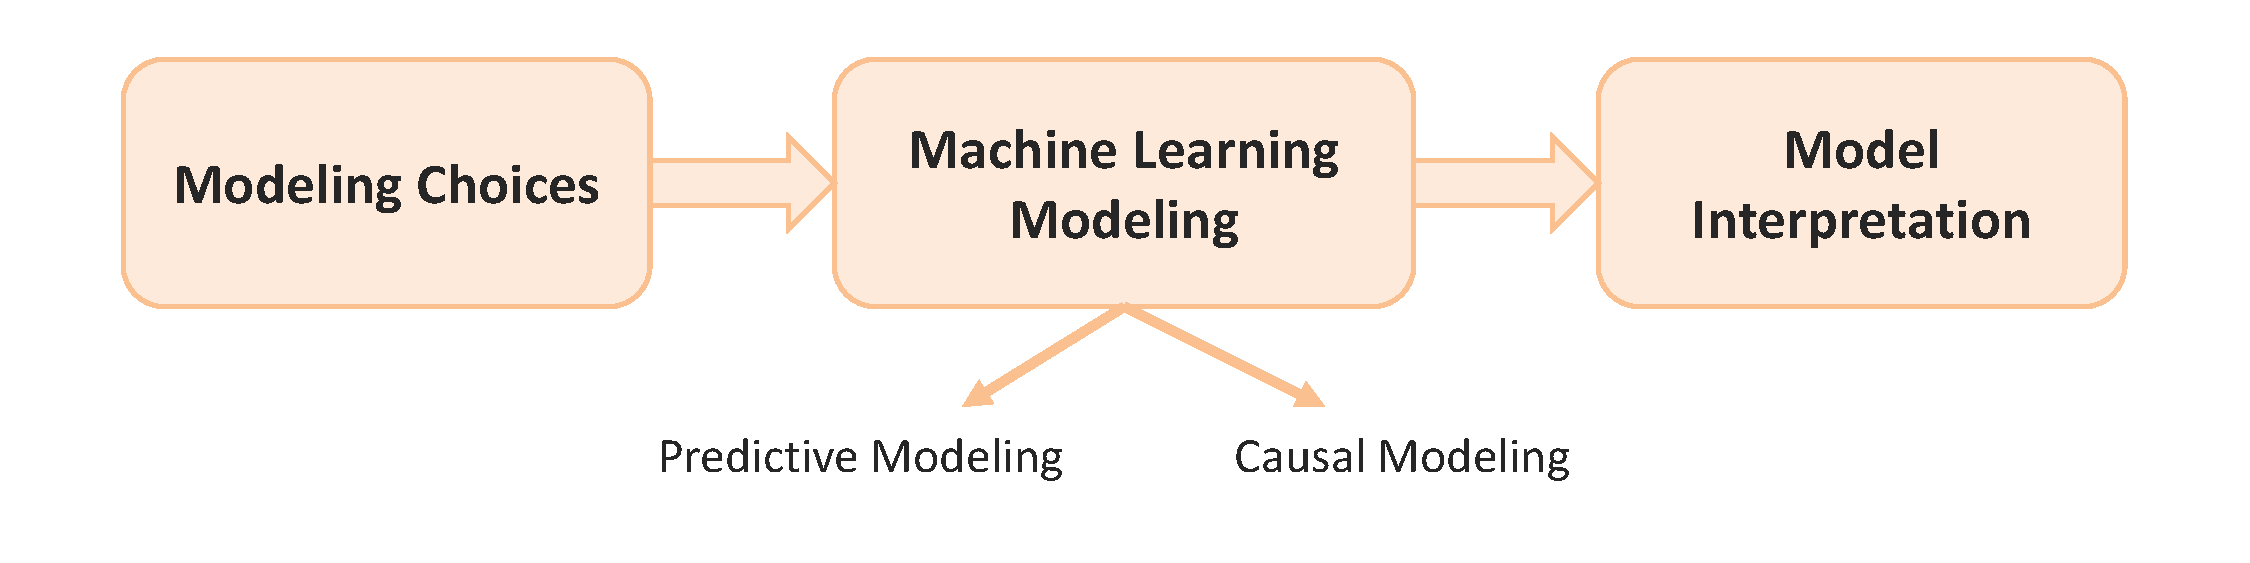
\includegraphics[width=6.5in]{ch1Fig1.pdf}
\caption{Illustration for the typical machine learning modeling pipeline.}
\label{Fig1Ch1}
\end{figure} 

Central to our proposed ML models is the idea of \textit{automation}. In Chapters 4 and 5, we develop methods for making modeling choices in a completely data-driven fashion for both the corss-sectional and longitudinal setups, without the need for manual tuning or expert intervention. Through these automated methods, the ML system is able to craft the model structure by itself so that it best fits the dataset at hand, thereby guarding against na\"ive modeling decisions that may bottleneck the model's predictive accuracy.   \\  
\\ 
\textbf{Stage 2: Machine Learning Modeling}\\
At the core of the modeling pipeline is the actual ML model being used to make predictions. For simple supervised prediction tasks, such as predicting a patient's risk of cardiovascular disease or diabetes based on their age and lifestyle-related variables, one can simply use standard off-the-shelf regression or classification models \cite{weng2017can}. However, many clinical questions cannot be simply reduced to a straightforward prediction problem. As we discuss in detail in Chapter 2, in many cases we would be interested in answering questions such as ``\textit{What is the effect of a given treatment on an individual patient?}'', ``\textit{What is the best treatment option for the patient at hand?}'', or ``\textit{Would this patient have better outcomes had they received a
different medication?}'' For this type of questions, the answer requires inferring the causal effects of interventions, which in turn requires inferring the patient outcomes in counter-factual scenarios that are not observed in the data \cite{morgan2015counterfactuals}. Thus, our core ML models must be able to carry out causal inference tasks and not just predictive inference ones.    

The ML modeling stage should account only for a broad range of clinical questions, but also for different data formats. In the cross-sectional setup, data is simply a static array of variables characterizing the patient state at a given point of time, whereas in the longitudinal setup, data is (irregularly) collected for every patient over time, and each patient may have a different number of observations.  \\ 
\\
\textbf{Stage 3: Model Interpretation}\\
Once the appropriate modeling choices have been made (stage 1), and a model has been trained using the available data (stage 2), we have a functioning ML pipeline in the pragmatic sense --- i.e., we have a model that makes the predictions that we are interested in. However, in almost all clinical setups, this is not enough. An accurate but inscrutable ML model may fail to gain patient and clinician trust. In fact, the conspicuous reluctance of many clinical researchers and epidemiologists to use ML models is often attributed to these models' ``black-box'' nature, which hinders their transparency and interpretability \cite{guidotti2019survey}. 

Because decision support systems based on ML models will be used to inform critical decision-making, clinicians and patients must be able to understand what these models have learned from data and how they makes their predictions. Various regulatory committees have even listed the transparency and intelligibility of prognostic models as a requirement for their deployment \cite{kattan2016american}. The final stage of the ML pipeline thus comprises an interpretation method that enables the users of the ML model to understand its predictions. This stage is inextricable from the preceding stages --- the appropriate kind of model interpretation depends on the ML model being used and format of the data used to train this model. 

\subsection{Outline of the Dissertation}
The rest of this dissertation is organized around the ML pipeline in Figure \ref{Fig1Ch1}. For both the cross-sectional and longitudinal setups, we develop models and algorithms that belong in different stages of the ML pipeline. The dissertation is divided into two parts: the first part (Chapters 2-5) focuses on our technical contributions with respect to developing ML tailored to healthcare applications, and the second part (Chapters 6-8) applies these methods to real-world clinical data. In what follows, we provide a sneak peek into each of the upcoming chapters, and explain how it relates to the high-level vision in Figure \ref{Fig1Ch1}.  

\label{Sec112}
\subsubsection{Models for Cross-sectional Data} % Technical notation and Figures
Chapters 2, 3 and 4 deal with the 3 stages of the ML pipeline in the cross-sectional setup. In this setup, we examine the relationship between a health outcome $Y$ (e.g., prevalence of a disease, survival outcomes, etc) and patient features $X$ by taking a static ``snapshot of a population'' at a single point of time. (Note that our notion of a ``cross-sectional setup'' corresponds to what is known in the epidemiological literature as \textit{observational studies}, which covers cohort, cross-sectional, and case-control studies.) Chapter 2 starts off with the~core component of the pipeline (stage 2), where we develop a comprehensive framework for ML-based models for causal effect estimation. Chapter 3 proceeds by providing~a~novel symbolic approach for interpreting the predictions of any black-box ML model (stage 3). In Chapter 4, we conclude the ML pipeline for cross-sectional data by developing an algorithm for automating the predictive and causal modeling choices.

\subsubsection{Models for Longitudinal Data}
In Chapter 5, we study the longitudinal setup. In this setup, we are presented sequential data of the form $X_1,.\,.\,.,X_t$ collected for patients who were followed up over an extended period of time. When dealing with longitudinal data, our goal is typically to capture disease trajectories in order to predict patient prognoses in a dynamic fashion and understand the underlying disease mechanisms and dynamics. Unlike in the cross-sectional setup where, in Chapter 5 we do not analyze each stage of the pipeline separately, but rather develop a single comprehensive model for sequential data that executes all stages of the pipeline jointly.     

\subsubsection{Clinical Application}
In Chapters 6, 7, and 8, we present a summary of the clinical studies that we conducted based on the ML models developed in earlier chapters. In these studies, we applied our models to cross-sectional data from large-scale cohorts of breast cancer, cardiovascular disease and cystic fibrosis patients, and longitudinal data from the UK cystic fibrosis registry.

\section{Summary of Technical Contributions}
In what follows, we present a brief summary of the technical contributions of each of the upcoming chapters with respect to existing literature.

\label{Sec12}
\subsection*{Chapter 2 Contributions}
In Chapter 2, we consider the problem of using ML to estimate the \textit{causal effect} of a treatment on individual patients on the basis of retrospective, observational data (causal modeling in stage 2 of the pipeline). This problem differs fundamentally from supervised learning since we never observe the treatment effects in the observational data --- we only observe the outcomes of a patient with or without the treatment, but never both. Despite a variety of recently proposed algorithmic solutions to this problem, a principled guideline for building estimators of treatment effects using machine learning algorithms is still lacking. In this chapter, we provide such guidelines by characterizing the fundamental limits of estimating heterogeneous treatment effects, establishing conditions under which these limits can be achieved, and building a practical algorithm for estimating treatment effects based on Gaussian processes. 

\subsection*{Chapter 3 Contributions}
In this Chapter, we tackle stage 3 of the pipeline: understanding the predictions of a general ML model. To this end, we introduce the \textit{symbolic metamodeling} framework --- a general methodology for interpreting predictions by converting ``black-box'' models into ``white-box'' functions that are understandable to human subjects. A symbolic metamodel is a model of a model, i.e., a surrogate model of a trained (machine learning) model expressed through a succinct symbolic expression that comprises familiar mathematical functions and can be subjected to symbolic manipulation. We parameterize metamodels using Meijer $G$-functions --- a class of complex-valued contour integrals that depend on real-valued parameters, and whose solutions reduce to familiar algebraic, analytic and closed-form functions for different parameter settings. This parameterization enables efficient optimization of metamodels via gradient descent, and allows discovering the functional forms learned by a model with minimal a priori assumptions. We show that symbolic metamodeling provides a generalized framework for model interpretation — many common forms of model explanation can be analytically derived from a symbolic metamodel.

\subsection*{Chapter 4 Contributions}
This Chapter addresses stage 1 of the pipeline. We developed an algorithm for automating the design of predictive and causal modeling tailored for clinical prognosis. Our algorithm optimizes ensembles of model configurations efficiently using a novel batched Bayesian optimization (BO) algorithm that learns a low-dimensional decomposition of the models' high-dimensional hyper-parameter space in concurrence with the BO procedure. This is achieved by modeling the models' performances as a black-box function with a Gaussian process prior, and modeling the ``similarities'' between the pipelines' baseline algorithms via a sparse additive kernel with a Dirichlet prior. For causal models, we propose an influence function-based approach to estimate their accuracy.

\subsection*{Chapter 5 Contributions}
Chapter 5 focuses on the longitudinal setup, where we develop a sequential model for predicting patient outcomes and understanding disease dynamics. Existing models provide the patient with pragmatic (supervised) predictions of risk, but do not provide the clinician with intelligible (unsupervised) representations of disease pathology. In this Chapter, we develop the \textit{attentive state-space model}, a deep probabilistic model that learns accurate and interpretable structured representations for disease trajectories. Unlike Markovian state-space models, in which state dynamics are memoryless, our model uses an attention mechanism to create ``memoryful'' dynamics, whereby attention weights determine the dependence of future disease states on past medical history. To learn the model parameters from medical records, we develop an inference algorithm that jointly learns a compiled inference network and the model parameters, leveraging the attentive representation to construct a variational approximation of the posterior state distribution. 

\part{Machine Learning for Individualized Medicine}

\chapter{Estimating Treatment Effects from Observational Data}

We start off with the core component of the ML pipeline: ML modeling. There is~already~a~wide range of well-established, off-the-shelf predictive models, hence we focus on \textit{causal modeling}. The problem of estimating heterogeneous (individualized) causal effects of a treatment from observational data is central in public health and drug development \cite{foster2011subgroup}. The increasing availability of observational data in these domains has encouraged the development of various machine learning algorithms tailored for inferring treatment effects using observational data (e.g. \cite{li2017matching,wager2017estimation,shalit2016estimating,alaa2017bayesian}). Due to the peculiarity of the treatment effect estimation problem, these algorithms address various modeling aspects that are foreign to standard supervised learning setups; such aspects include ways to handle \textit{sample selection bias} \cite{heckman1977sample}, and ways to model \textit{treated} and \textit{untreated} data points. Despite a variety of recent algorithmic approaches, principled guidelines for model design are lacking. 

In this Chapter, we identify guiding principles for designing practical treatment effect estimation algorithms in the context of Bayesian nonparametric inference, and propose one an algorithm that follows these guidelines. We set these guidelines by characterizing the fundamental limits of estimating treatment effects, and studying the impact of various common modeling choices on the achievability of those limits. In what follows, we provide a brief technical background for the treatment effect estimation problem, along with a summary of our contributions. 

\section{Background and Summary of Contributions}
\label{ch2sec1}
Our analysis hinges on the Rubin-Neyman potential outcomes model \cite{rubin2005causal}. That is, we consider an observational dataset with a population of subjects, where each subject $i$ is endowed with a $d$-dimensional feature $X_i \in \mathcal{X}$. We assume that $\mathcal{X} = [0,1]^d$, but most of our results hold for general compact metric spaces (bounded, closed sets in $\mathbb{R}^d$). A treatment assignment indicator $W_i \in \{0,1\}$ is associated with subject $i$; $W_i = 1$ if the treatment under study was applied to subject $i$, and $W_i = 0$ otherwise. Subject $i$'s responses with and without the treatment (the potential outcomes) are denoted as $Y^{\mbox{\tiny $(1)$}}_i$ and $Y^{\mbox{\tiny $(0)$}}_i$, respectively. Treatments are assigned to subjects according to an underlying policy that depends on the subjects' features, i.e. $W_i \not\!\perp\!\!\!\perp X_i$. This dependence is quantified via the conditional distribution $p(x) = \mathbb{P}(W_i=1|X_i=x)$, also known as the \textit{propensity score} of subject $i$ \cite{rosenbaum1984reducing}. The response $Y^{\mbox{\tiny $(W_i)$}}_i$ is the ``factual outcome" which we observe in the data, whereas $Y^{\mbox{\tiny $(1-W_i)$}}_i$ is the unrealized ``counterfactual outcome" \cite{bottou2013counterfactual}. An observational dataset $\mathcal{D}_n$ comprises $n$ samples of the form: 
\begin{align}
\mathcal{D}_n = \{X_i, W_i, Y^{\mbox{\tiny $(W_i)$}}_i\}_{i=1}^n\,\, 
\label{ch2eq1}
\end{align}
The causal effect of the treatment on subject $i$ with a feature $X_i = x$ is characterized through the \textit{conditional average treatment effect} (CATE) function $T(x)$, which is defined as the expected difference between the two potential outcomes \cite{rubin2005causal}, i.e. 
\begin{align}
T(x) = \mathbb{E}\big[\, Y^{\mbox{\tiny $(1)$}}_i-Y^{\mbox{\tiny $(0)$}}_i\,|\,X_i = x\,\big]
\label{ch2eq2}
\end{align}
Our goal is to identify a set of guiding principles for building estimators of the CATE $T(x)$ using samples from $\mathcal{D}_n$. Throughout this Chapter, we will assume that the density $d\mathbb{P}(X_i,W_i,Y^{\mbox{\tiny $(0)$}}_i,Y^{\mbox{\tiny $(1)$}}_i)$ supports the assumptions of \textit{unconfoundedness} and \textit{overlap}, which are necessary for causal identifiability and consistency. Unconfoundedness requires that  $(Y^{\mbox{\tiny $(0)$}}_i,Y^{\mbox{\tiny $(1)$}}_i) \!\perp\!\!\!\perp W_i\,|\,X_i$, whereas overlap requires that $0 < p(x) < 1$ \cite{rosenbaum1984reducing}. \textbf{Selection bias} occurs in $\mathcal{D}_n$ since the distribution of the treated/control subjects does not match that of the overall population.

In order to come up with principled guidelines for building estimators of $T(x)$, we characterize the fundamental (information-theoretic) limits of estimating the CATE using samples from $\mathcal{D}_n$, and identify the modeling choices that would allow achieving those limits. To this end, in \textbf{Section \ref{ch2sec3}} we tackle the following question: \textbf{what are the fundamental limits of CATE estimation?} We answer this question by deriving the \textit{optimal minimax rate} for estimating $T(x)$ using $\mathcal{D}_n$. Interestingly, it turns out that the optimal rate \textbf{does not} depend on \textbf{selection bias}, but rather on the \textbf{smoothness} and \textbf{sparsity} of the more ``complex" of the functions $\mathbb{E}[\, Y^{\mbox{\tiny $(0)$}}_i\,|\,X_i = x\,]$ and $\mathbb{E}[\, Y^{\mbox{\tiny $(1)$}}_i\,|\,X_i = x\,]$. We focus our analysis on Bayesian nonparametric methods, since they have the appealing properties of being robust to misspecification and are accessible for theoretical analysis. 

Our analysis reveals that the relative importance of the different modeling aspects vary with the sample size. In particular, in the \textbf{large-sample regime}, selection bias does not pose a serious problem, and the model's performance would be mainly determined by its \textbf{structure}, i.e. the way the outcomes $Y^{\mbox{\tiny $(0)$}}_i$ and $Y^{\mbox{\tiny $(1)$}}_i$ are modeled, and the impact of that on variable selection and hyperparameter tuning. On the contrary, selection bias can seriously harm a model's generalization performance in \textbf{small-sample regimes}. A good model should then be carefully designed so that it operates well in both regimes by possessing the right \textbf{model structure} that would allow learning at a fast rate, and the right \textbf{model selection} (hyperparameter optimization) scheme that would account for selection bias. 
   
In Section \ref{ch2sec4}, we build a practical CATE estimation algorithm guided by the results of the analyses in Section \ref{ch2sec3}. We model the outcomes $Y^{\mbox{\tiny $(0)$}}_i$ and $Y^{\mbox{\tiny $(1)$}}_i$ using a Gaussian process with a \textit{non-stationary} kernel that captures the different relevant variables and different levels of smoothness of the functions $\mathbb{E}[\, Y^{\mbox{\tiny $(0)$}}_i\,|\,X_i = x\,]$ and $\mathbb{E}[\, Y^{\mbox{\tiny $(1)$}}_i\,|\,X_i = x\,]$. We prove that this model structure can achieve the optimal rate of CATE estimation when tuned with the right hyperparameters. We also propose a \textit{doubly-robust} hyperparameter optimization scheme that accounts for selection bias in small-sample regimes, without hindering the model's minimax-optimality in the large sample limit. We show that our algorithm outperforms state-of-the-art methods using a well-known semi-synthetic simulation setup.

\section{Related Work}
Very few works have attempted to characterize the limits of CATE estimation, or study the impact of different modeling choices on the CATE estimation performance in a principled manner. \cite{alaa2017bayesian2} characterized the asymptotic ``information rates" for different CATE estimators, but provided no clear guidelines on practical model design or an analysis of the impact of sample selection bias. The study in \cite{kunzel2017meta} was rather empirical in nature, comparing the performance of different regression structures for the potential outcomes while ignoring selection bias. A similar study, but focusing only on random forest models, was conducted in \cite{lu2017estimating}.   

Most of the previous works have been algorithmic in nature, focusing mainly on devising algorithms that correct for selection bias (e.g. \cite{johansson2016learning,jjschaar,wager2017estimation,li2017matching}). Some of these works cast the selection bias problem as a problem of \textit{covariate shift} \cite{sugiyama2007covariate}, and use techniques from \textit{representation learning} to learn feature maps that balance the biased data (e.g. \cite{li2017matching,shalit2016estimating,johansson2016learning}). However, those works report much bigger improvements in CATE estimation when changing their model structure (e.g. architecture of a neural network), as compared to the gains attained by only accounting for bias (see the comparisons between the TARnet and BNN models in \cite{shalit2016estimating}). Similar observations are reported in \cite{alaa2017bayesian,Onur1}, where the selection of the model structure seemed to influence the achieved CATE estimation performance even when selection bias is not accounted for. However, none of these works offer a discussion on whether selection bias is actually the main challenge in CATE estimation, or whether the outcomes' model structure may have a bigger influence on performance.

In contrast to the works above, in this Chapter we do not attempt to develop a model by presupposing that particular modeling aspects are of greater importance than others, but rather provides a framework for understanding the limits on the achievable performance, and how different modeling aspects influence a model's chance of achieving those limits. We use our analyses to both reflect on the modeling choices made in the works above, and also devise a novel, principled CATE estimation algorithms that achieves the fundamental performance limits.  

\section{Estimating CATE: Problem Setup} 
\label{ch2sec3}
\subsection{Potential Outcomes and Propensity Score}
\label{pO22}
We consider the following \textit{random design} regression model for the potential outcomes:
\begin{equation}
Y^{\mbox{\tiny $(w)$}}_i = f_{w}(X_i) + \varepsilon_{i,w},\, w \in \{0,1\},  
\label{ch2eq3}
\end{equation}
where $\varepsilon_{i,w} \sim \mathcal{N}(0,\sigma^2_{w})$ is a Gaussian noise variable. It follows from (\ref{ch2eq2}) that the CATE is $T(x) = f_{1}(x)-f_{0}(x)$. The \textit{response surfaces} $f_{1}(x)$ and $f_{0}(x)$ correspond to the subjects' responses with and without the treatment. We assume that $f_{w}(.): \mathcal{X} \rightarrow \mathbb{R}$, $w \in \{0,1\}$, is a totally bounded function that lives in a space of ``smooth" or ``regular" functions, with an unknown smoothness parameter $\alpha_{w}$. We use H\"older balls for concreteness, although our results extend to other function spaces. A function $f_{w}(.)$ lies in the H\"older ball $H^{\alpha_{w}}$, with a H\"older exponent $\alpha_{w} > 0$, if and only if it is bounded in sup-norm by a constant $C > 0$, all its partial derivatives up to order $\lfloor \alpha_{w} \rfloor$ exist, and all its partial derivatives of order $\lfloor \alpha_{w} \rfloor$ are Lipschitz with exponent $(\alpha_{w}-\lfloor \alpha_{w} \rfloor)$ and constant $C$. The H\"older exponents quantify the complexities of $f_0$ and $f_1$, and hence the hardness of estimating $T(x)$ would depend on $\alpha_{0}$ and $\alpha_{1}$. 

\subsection{Bayesian Nonparametric Inference}
Nonparametric inference is immune to misspecification of the outcomes' and propensity models \cite{kennedy2018nonparametric}, and hence we focus on Bayesian nonparametric methods for inferring $T(.)$ on the basis of $\mathcal{D}_n$. Bayesian inference entails specifying a prior distribution $\Pi$ over $f_1(.)$ and $f_0(.)$, i.e.
\begin{equation}
f_0, f_1 \sim \Pi(\bar{\varphi}_{\beta_0}, \bar{\varphi}_{\beta_1}),
\label{ch2eq4}
\end{equation}
where $\bar{\varphi}_{\beta_w} = \{\varphi^k_{\beta_w}\}_{k=1}^\infty, w \in \{0,1\},$ are complete orthonormal bases (indexed by a parameter $\beta_w > 0$) with respect to Lebesgue measure in $\mathcal{X}$, $f_w = \sum_k \bar{f}^k_w \cdot \varphi^k_{\beta_w},$ and $\bar{f}^k_w = \langle f_w, \varphi^k_{\beta_w}\rangle$. Thus, for given bases $\bar{\varphi}_{\beta_0}$ and $\bar{\varphi}_{\beta_1}$, $\Pi$ places a probability distribution on the projections $\{\bar{f}^k_w\}_k$. Potential choices for the basis $\bar{\varphi}_{\beta_w}$ that would give rise to implementable Bayesian inference algorithms include regular wavelet basis \cite{zhang1997using}, radial basis for a reproducing kernel Hilbert space (RKHS) \cite{van2008reproducing}, etc. In general, $\beta_w$ would determine the smoothness of the function space spanned by $\bar{\varphi}_{\beta_w}$. 

\subsection{Towards Principled CATE Estimation} 
To evaluate the predictive accuracy of the Bayesian inference procedure, we analyze the ``frequentist" loss of point estimators $\hat{T}(x)$ induced by the Bayesian posterior $d\Pi_n(T(x)\,|\,\mathcal{D}_n)$, assuming that $\mathcal{D}_n$ is generated based on fixed, \textit{true} response surfaces $f_{1}(x)$ and $f_{0}(x)$. (This type of analysis is sometimes referred to as the ``Frequentist-Bayes" analysis \cite{sniekers2015adaptive}.) In particular, we quantify the performance of a point estimator $\hat{T}(x) = \delta(d\Pi_n(T(x)\,|\,\mathcal{D}_n))$ by its squared-$L^2(\mathbb{P})$ error, which was dubbed the \textit{precision of estimating heterogeneous effects} \textbf{(PEHE)} in \cite{hill2011bayesian}, and is formally defined as:
\begin{align}
\mathbold{\psi}(\hat{T}) &\triangleq \mathbb{E}\,\|\,\hat{T} - T\,\|^2_{\mbox{\tiny $L^2(\mathbb{P})$}}, 
\label{ch2eq5}
\end{align} 
where $L^2(\mathbb{P})$ is the $L^2$ norm with respect to $\mathbb{P}(X)$, i.e. $\|f(x)\|^2_{\mbox{\tiny $L^2(\mathbb{P})$}} = \int f^2(x)\, d\mathbb{P}(X=x)$.

The ``fundamental problem of causal inference" is that for every subject $i$ in $\mathcal{D}_n$, we only observe the \textbf{factual} outcome $Y^{\mbox{\tiny $(W_i)$}}_i$, whereas the \textbf{counterfactual} $Y^{\mbox{\tiny $(1-W_i)$}}_i$ remains unknown, which renders empirical evaluation of the PEHE in (\ref{ch2eq5}) impossible. Moreover, $\mathcal{D}_n$ would generally exhibit sample \textbf{selection bias} \cite{heckman1977sample}, because the treatment assignment mechanism (decided by $p(x)$) creates a discrepancy between the feature distributions of the treated/control population and the overall population. Thus, standard \textbf{supervised learning} approaches based on empirical risk minimization cannot be used to learn a generalizable model for the CATE from samples in $\mathcal{D}_n$. This gives rise to the following fundamental modeling questions that are peculiar to CATE estimation:
\begin{itemize} % HOW DO THEY RELATE TO THE PRIOR
\item \textbf{[Q1]:} How should the treatment assignment $W_i$ be incorporated into the learning model? % structure of the prior
\item \textbf{[Q2]:} How should selection bias be handled? % how to adapt the prior
\end{itemize}

Adequate answers to \textbf{[Q1]} and \textbf{[Q2]} would provide guidelines for selecting the prior $\Pi(\bar{\varphi}_{\beta_0}, \bar{\varphi}_{\beta_1})$. Addressing the modeling questions above requires a profound understanding of the \textbf{fundamental limits} of CATE estimation, in addition to an understanding of the impact of different modeling choices on the \textbf{achievability} of such limits. The next Sections provide principled answers to \textbf{[Q1]} and \textbf{[Q2]} by addressing the following, more fundamental questions:
\begin{itemize}
\item \textbf{\underline{Section \ref{ch1sec3}}: What are the \textit{limits} on the performance achieved by \textit{any} CATE estimator?}
\item \textbf{\underline{Section \ref{ch2sec4}}: How can we build \textit{practical algorithms} that can achieve these limits?}
\end{itemize}

\section{Fundamental Limits of CATE Estimation} %1 Theorem, 2- Holder codewords and hamming 3- remarks
\label{ch1sec3} 
In this Section, we establish an information-theoretic limit on the performance of \textit{any} CATE estimator. In what follows, we use the standard Bachmann-Landau order notation, and write $a \vee b = \max\{a,b\},$ $a \wedge b = \min\{a,b\}$. The notation $a \lesssim b$ means that $a \leq C b$ for a universal constant $C$, and $\asymp$ denotes asymptotic equivalence. 

\subsection{Optimal Minimax Rates}
\label{BMS2}
The ``hardness" of a nonparametric estimation problem is typically characterized by its \textit{minimax} risk \cite{stone1982optimal}, i.e. the minimum worst case risk achieved by \textit{any} estimator when the estimand is known to live in a given function space \cite{yang2015minimax}. In the following Theorem, we establish the optimal minimax rate for the PEHE risk in terms of the complexity of the response surfaces $f_0$ and $f_1$.\\ 
\\
\textbf{Theorem~1.} \textit{Suppose that $\mathcal{X} = [0,1]^d$, and that $f_w$ depends on a subset of $d_w$ features with $d_w \leq \min\{n,d\}$ for $w \in \{0,1\}$. If $f_0 \in H^{\alpha_0}$ and $f_1 \in H^{\alpha_1}$, then the optimal minimax rate is:} 
\begin{align}
\inf_{\hat{T}} \sup_{f_0,f_1} \mathbold{\psi}(\hat{T}) \,\asymp\, \underbrace{n^{-\left(1+\frac{1}{2}\left(\frac{d_0}{\alpha_0}\vee \frac{d_1}{\alpha_1}\right)\right)^{-1}}}_{\textbf{CATE\,\, estimation}} \vee \underbrace{\log \mbox{\footnotesize$\left(\frac{d^{d_0+d_1}}{d_0^{d_0}\, d_1^{d_1}}\right)^{\frac{1}{n}}$}.}_{\textbf{Variable\,\, selection}}\nonumber
\end{align} 
\textit{The above holds for any $p(.) \in H^{\alpha_p}$, $\alpha_p > 0$.} \,\,\, $\mathbf{\Box}$ \\

In Theorem 1, the supremum is taken over $\alpha_w$-H\"older balls ($w \in \{0,1\}$), whereas the infimum is taken over all possible Bayesian estimators. The~minimax~rate~in~Theorem~1 corresponds to the \textbf{fastest rate} by which \textbf{any} (Bayesian) estimator $\hat{T}(.)$ can approximate the CATE function $T(.)$. The proof of Theorem 1 uses information-theoretic techniques based on Fano's method to derive algorithm-independent estimation rates \cite{yang1999information}. In the following set of remarks, we revisit \textbf{[Q1]} and \textbf{[Q2]} in the light of the results of Theorem 1.\\ 
\\ 
\textbf{How can Theorem 1 help us address \mbox{\footnotesize \textbf{[Q1]}} and \mbox{\footnotesize \textbf{[Q2]}}?}\\
\\
$\triangleright$ \textbf{Remark 1 (Smoothness and sparsity)}

Theorem 1 says that estimating CATE is as hard as nonparametric regression for functions with additive sparsity \cite{raskutti2009lower,yang2015minimax}. The minimax rate in Theorem 1 decomposes into a term reflecting the complexity of CATE estimation under correct variable selection for $f_0$ and $f_1$, and a term reflecting the complexity of variable selection. Variable selection complexity remains small as long as $\log(d) = \Theta(n^\zeta),$ for some $\zeta \in (0,1)$, and approaches the parametric rates as $\zeta \to 0$. The minimax rate will generally be dominated by the complexity of CATE estimation, and will approach the parametric rates only for very smooth response surfaces with small number of relevant dimensions, i.e. $\frac{d_0}{\alpha_0} \vee \frac{d_1}{\alpha_1} \to 0$.    

The main takeaway from Theorem 1 is that the CATE learning rate is determined by the more ``complex" of the surfaces $f_0$ and $f_1$, where complexity is quantified by the sparsity-to-smoothness ratio $d_w/\alpha_w$ for $w \in \{0,1\}$. Thus, a model would achieve the optimal CATE learning rate only if it selects the correct relevant variables for $f_0$ and $f_1$, and tunes its ``hyperparameters" (i.e. smoothness of the prior) to cope with a complexity of $\frac{d_0}{\alpha_0} \vee \frac{d_1}{\alpha_1}$. When $\frac{d_0}{\alpha_0}$ and $\frac{d_1}{\alpha_1}$ are very different (e.g. $f_0$ and $f_1$ have different relevant features), rate-optimal estimation is possible only if the model incorporates such differences in $\Pi(\bar{\varphi}_{\beta_0},\bar{\varphi}_{\beta_1})$. % bases

The discussion above \textbf{provides a concrete answer to \mbox{\footnotesize \textbf{[Q1]}}:} the treatment assignment variable $w$ should be incorporated into the model in such a way that it \textbf{encodes the different relevant dimensions and smoothness levels of $\boldsymbol{f_0}$ and $\boldsymbol{f_1}$ in the bases $\boldsymbol{\bar{\varphi}_{\beta_0}}$ and $\boldsymbol{\bar{\varphi}_{\beta_1}}$}. (The simplest way to achieve this is to use two separate models for $f_0$ and $f_1$.) This is not fulfilled by many of the previous models that built a single regression function of the from $f: \mathcal{X} \times \{0,1\} \to \mathbb{R}$, and estimated the CATE as $\hat{T}(x) = f(x,1) - f(x,0)$ \cite{hill2011bayesian,johansson2016learning,powers2017some}. This is because such models enforced the smoothness of the prior along all features to be the same for $w = 0$ and $w = 1$.\\ 
\\    
$\triangleright$ \textbf{Remark 2 (Selection bias)} 

Theorem 1 gives a rather surprising answer to \textbf{[Q2]}: the \textbf{optimal learning rate} is \textbf{oblivious to selection bias}. Such a finding is consistent with previous results on nonparametric kernel density estimation under selection bias \cite{borrajo2017bandwidth}, and parametric Bayesian inference under \textit{covariate shift} \cite{shimodaira2000improving,sugiyama2007mixture}. It shows that many of the recent works have missed the target; the works in \cite{johansson2016learning,shalit2016estimating,alaa2017bayesian} cast the problem of CATE estimation as one of \textbf{covariate shift} that results from selection bias. However, Theorem 1 says that selection bias is not a problem when we have a sufficiently large amount of data. This is because selection bias is inherently a misspecification problem, and hence its impact on nonparametric inference is washed away in large-sample regimes. 

Remarks 1 and 2 posit an explanation for various recurrent (empirical) findings reported in previous literature. For instance, \cite{hahn2017bayesian} found that separate modeling of $f_0$ and $f_1$ via Bayesian additive regression trees (BART) outperforms the well-known single-surface BART model developed in \cite{hill2011bayesian}. Similar findings were reported for models based on Gaussian processes \cite{alaa2017bayesian}, and models based on deep neural networks \cite{shalit2016estimating}. All such findings can be explained in the light of Remark 1. On the other hand, Remark 2 may provide an explanation as to why the ``TARnet" model in \cite{shalit2016estimating}, which models $f_0$ and $f_1$ using separate neural networks and does not account for selection bias, outperformed the ``BNN" model in \cite{johansson2016learning}, which regularizes for selection bias but fits a single-output network for $f_0$ and $f_1$. 

\subsection{Backing off from ``Asymptopia"} 
\label{backasymp}
Theorem 1 shows that selection bias does not hinder the optimal minimax rates, and that it is only the structural properties of the prior $\Pi(\bar{\varphi}_{\beta_0},\bar{\varphi}_{\beta_1})$ that determine a model's rate of learning. But does the achieved learning rate suffice as a sole criterion for addressing the modeling questions \textbf{[Q1]} and \textbf{[Q2]}? The answer is ``yes" only if $\mathcal{D}_n$ comes from a large observational dataset, in which case the learning rate suffices as a descriptor for the large-sample performance. However, if $\mathcal{D}_n$ is small, which is typical in post-hoc analyses of clinical trials \cite{foster2011subgroup}, then one should make the design choices that would optimize the small-sample performance. In order to give a complete picture of the performance in large and small-sample regimes, we derive the following bound on the PEHE:
\begin{align}
\mathbold{\psi}(\hat{T}) &\leq \bar{C}\cdot \exp(D_2(Q_0\,\|\,Q))\cdot\|f_0-\hat{f}_0\|^2_{L^2(\mathbb{P}_0)} + \bar{C}\cdot \exp(\underbrace{D_2(Q_1\,\|\,Q)}_{\substack{\textbf{Reyni}\\ \textbf{Divergence}}})\cdot\underbrace{\|f_1-\hat{f}_1\|^2_{L^2(\mathbb{P}_1)}}_{\substack{\textbf{Supervised}\\ \textbf{learning\,\,loss}}},
\label{ch2eq7} 
\end{align}	
for some $\bar{C} > 0$, where $L^2(\mathbb{P}_w)$, for $w \in \{0,1\},$ is the $L^2$ norm with respect to $d\mathbb{P}(X=x\,|\,W=w)$, $Q = d\mathbb{P}(X=x)$, $Q_w = d\mathbb{P}(X=x\,|\,W=w)$, and $D_{m}(p\,\|\,q)$ is the $m^{th}$ order R\'eyni divergence. The bound in (\ref{ch2eq7}) holds for all $n > 0$, and is tight (refer to the Appendix); it shows that the PEHE is a weighted linear combination of the mean squared losses for the two underlying supervised problems of learning $f_0$ and $f_1$ with \textbf{no covariate shift}, where the weights are determined by the extent of the mismatch between the distributions of the treated and control populations, quantified by the R\'eyni divergence measure. If $\mathcal{D}_n$ is a dataset obtained from a randomized controlled trial ($Q=Q_0=Q_1$), then we have $D_2(Q_0\,\|\,Q)=D_2(Q_1\,\|\,Q) = 0$, and the bound boils down to a sum of two supervised learning losses, i.e. $\mathbold{\psi}(\hat{T}) \leq \bar{C}\cdot\|f_0-\hat{f}_0\|^2_{L^2(\mathbb{P})} + \bar{C}\cdot\|f_1-\hat{f}_1\|^2_{L^2(\mathbb{P})}$.

Since the minimax rate for standard nonparametric regression is $\|f_w-\hat{f}_w\|^2_{2} \asymp C_w \cdot n^{\frac{-2\alpha_w}{2\alpha_w + d_w}}$ \cite{stone1982optimal}, when $d_0/\alpha_0 >> d_1/\alpha_1$, the first-order Taylor approximation for the logarithm of the PEHE in (\ref{ch2eq7}) is given by:
\begin{align}
\log(\mathbold{\psi}(\hat{T})) \approx \, \underbrace{D_2(Q_0\|Q)}_{\substack{\textbf{Selection}\\ \textbf{bias}}} + \underbrace{\log(C_0)}_{\substack{\textbf{Bias}\\ \textbf{correction}}} - \underbrace{\frac{2\alpha_0}{2\alpha_0 + d_0}}_{\substack{\textbf{Learning\, rate}}}\log(n) +\, O\left(n^{\frac{-2\alpha_1}{2\alpha_1 + d_1}+\frac{2\alpha_0}{2\alpha_0 + d_0}}\right).
\label{ch2eq8}
\end{align}
That is, when viewed on a $\log$-$\log$ scale, the behavior of the PEHE versus the number of samples can be described as follows. $\log(\mbox{PEHE})$ is a linear function of $\log(n)$. Selection bias adds a constant offset to $\log(\mbox{PEHE})$, but does not affect its slope, which harms the performance only in the small-sample regime. In the large-sample regime, the slope of $\log(\mbox{PEHE})$, which depends solely on the smoothness and sparsity of the response surfaces, dominates the performance, and selection bias becomes less of a problem. Figure \ref{ch2fig1} depicts the PEHE in (\ref{ch2eq8}) on a $\log$-$\log$ scale.
		
\begin{figure}[t]
\centering
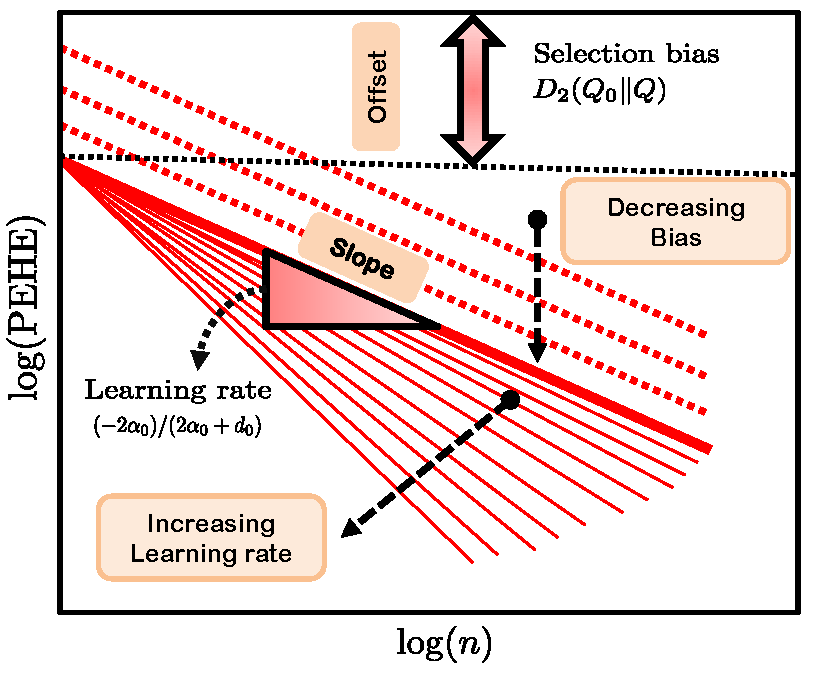
\includegraphics[width=3.5in]{logpehe.pdf}
\caption{The PEHE in (\ref{ch2eq8}) plotted on a $\log$-$\log$ scale.}
\label{ch2fig1}
\end{figure}
 
\section{CATE Estimation using Non-Stationary Gaussian Process Regression}
\label{ch2sec4}
In this Section, we build on the analyses conducted in Section \ref{ch1sec3} to design a practical algorithm for CATE estimation. 

\subsection{Non-Stationary Gaussian Process Priors} 
\label{ch2sec41} 
We specify the prior $\Pi(\bar{\varphi}_{\beta_0},\bar{\varphi}_{\beta_1})$ as a Gaussian process (GP) over $g: \mathcal{X} \times \{0,1\} \to \mathbb{R}$, with a kernel $\boldsymbol{K}_{\beta}$, and a hyperparameter set $\beta$ as follows:
\begin{align}  
g \sim \mathcal{GP}\left(0,\boldsymbol{K}_{\beta}(z,z^{\prime})\right),
\label{ch2eq9}
\end{align}
where $z = (x,w) \in \mathcal{X} \times \{0,1\},$ and $f_w(x) = g(x,w)$. The kernel $\boldsymbol{K}_{\beta}$ specifies the bases $\bar{\varphi}_{\beta_0}$ and $\bar{\varphi}_{\beta_1}$ through its induced canonical feature map $\boldsymbol{K}_{\beta}(.,z)$ \cite{rasmussen2006gaussian,alvarez2012kernels}. As pointed out in \textbf{Remark 1}, the treatment assignment variable $w$ should encode the different relevant dimensions and smoothness levels of $f_0$ and $f_1$. Thus, we model $\boldsymbol{K}_{\beta}$ as a \textit{non-stationary} kernel that depends on $w$ as follows:      
\begin{align}  
\boldsymbol{K}_{\beta}(z,z^{\prime}) &= \boldsymbol{\Gamma}(w,w^{\prime}) \cdot \boldsymbol{k}_{\beta}^{T}(x,x^{\prime}), \nonumber \\
\boldsymbol{k}_{\beta}(x,x^{\prime}) &= \left[k_{\beta_0}(x,x^{\prime}),k_{\beta_1}(x,x^{\prime}),k_{\beta_0}(x,x^{\prime}) + k_{\beta_1}(x,x^{\prime})\right], \nonumber \\
\boldsymbol{\Gamma}(w,w^{\prime}) &= \left[\Gamma_{0}(w,w^{\prime}),\Gamma_{1}(w,w^{\prime}),1-\Gamma_{0}(w,w^{\prime})-\Gamma_{1}(w,w^{\prime})\right], \nonumber
\end{align}
where $\Gamma_{0}(w,w^{\prime}) = (1-w)(1-w^{\prime})$, $\Gamma_{1}(w,w^{\prime}) = w\cdot w^{\prime}$, and $k_{\beta_w}(x,x^{\prime})$ is a Mat\'ern kernel with a length-scale parameter $\beta_w$, for $w \in \{0,1\}$. The kernel defined above ensures that any covariance matrix induced by points in $\mathcal{X}\times\{0,1\}$ is positive definite. Variable selection is implemented by using the \textit{automatic relevance determination} version of the Mat\'ern kernel \cite{rasmussen2006gaussian}. The non-stationarity of $\boldsymbol{K}_{\beta}$ allows setting \textbf{different} length-scales and relevant variables for the marginal priors on $f_0$ and $f_1$ while sharing data between the two surfaces, i.e.
\begin{align}  
\boldsymbol{K}_{\beta}((x,w),(x^{\prime},w)) &= k_{\beta_w}(x,x^{\prime}),\,\, w \in \{0,1\}, \nonumber \\
\boldsymbol{K}_{\beta}((x,w),(x^{\prime},w^{\prime})) &= k_{\beta_0}(x,x^{\prime}) + k_{\beta_1}(x,x^{\prime}),\, w \neq w^{\prime}.
\label{ch2eq10}
\end{align}

That is, all draws from the prior give Mat\'ern sample paths with different smoothness levels ($\beta_0$ and $\beta_1$) for $f_0$ and $f_1$, respectively, and the correlations between the paths are captured via the kernel mixture $k_{\beta_0}(x,x^{\prime}) + k_{\beta_1}(x,x^{\prime})$. Note that draws from a Mat\'ern prior with length-scale $\beta$ are almost surely $\bar{\beta}$-H\"older for all $\bar{\beta} \leq \beta$ \cite{vaart2011information}. Thus, $\mathcal{GP}(0,\boldsymbol{K}_{\beta})$ specifies a $\beta_w$-H\"older ball as an a priori regularity class for response surface $f_w,\, w \in \{0,1\}$. 

In the following Theorem, we show that point estimators induced by the prior $\mathcal{GP}(0,\boldsymbol{K}_{\beta})$ can achieve the optimal minimax rate in Theorem 1.\\
\\
\textbf{Theorem~2.} \textit{Suppose that the $d_w$ relevant features for $f_w$ are known a priori for $w \in \{0,1\}$. If $f_0 \in H^{\alpha_0}$, $f_1 \in H^{\alpha_1}$, $\Pi = \mathcal{GP}(0,\boldsymbol{K}_{\beta})$, and $\hat{T} = \mathbb{E}_{\Pi}[\,T\,|\,\mathcal{D}_n\,]$, then we have that} 
\begin{align}
\mathbold{\psi}(\hat{T}) \,\lesssim\, n^{-\frac{2(\alpha_0 \wedge \beta_0)}{2\beta_0 + d_0}} \vee n^{-\frac{2(\alpha_1 \wedge \beta_1)}{2\beta_1 + d_1}}  
\nonumber
\end{align} 
\textit{whenever $\min\{\alpha_0, \alpha_1, \beta_0, \beta_1\} \geq d/2$.} \,\,\, $\mathbf{\Box}$

Note that posterior consistency holds for all combinations of $(\alpha_0, \alpha_1, \beta_0, \beta_1)$ since the support of the Mat\'ern prior is the space of bounded continuous functions\footnote{This is because the RKHS associated with the prior lies dense in the space of bounded continuous functions \cite{van2008rates,van2008reproducing}.}. The bound in Theorem 2 can be shown to be tight using the results in \cite{castillo2008}. Theorem 2 says that the posterior induced by the prior $\mathcal{GP}(0,\boldsymbol{K}_{\beta})$ contracts around the true CATE function at the optimal rate given in Theorem 1 provided that the following \textbf{matching condition} is met:   
\begin{align}
\beta_v \,\,&= \alpha_v \nonumber \\
\alpha_{v}\frac{d_{1-v}}{d_v} \,\,&\leq \beta_{1-v} \leq \alpha_{1-v} + \frac{\alpha_{1-v}\cdot d_{v}}{2\alpha_{v}}-\frac{d_{1-v}}{2},
\label{ch2eq11}
\end{align}
where $v = 1$ if $d_1/\alpha_1 > d_0/\alpha_0$, and $v = 0$ otherwise. The condition in (\ref{ch2eq11}) implies that achieving the optimal rate (steepest slope in Figure \ref{ch2fig1}) via the non-stationary GP prior in Section \ref{ch2sec41} is only a matter of hyperparameter tuning: the smoothness of the prior needs to match the smoothness of the ``more complex" of the two response surfaces. Note that Theorem 2 implies that we do not need to handle selection bias in order to achieve the optimal rate, which is consistent with the earlier discussion in \textbf{Remark 2}. 
%%%%%%%%%%%%%%%%%%%%%%%%%%%%%%%%%%%%%%%%%%%%%%%%%%%%%%%%%%%%%%%%%%%%%%

\subsection{Doubly-Robust Hyperparameters}
\label{modsec}
Theorem 2 says that the optimal minimax rate for CATE estimation can be achieved by satisfying the smoothness matching condition in (\ref{ch2eq11}). However, in practice, the smoothness levels of the true response functions are unknown and need to be learned from the data. Moreover, since selection bias is impactful in small-sample regimes, ignoring it may lead to a poor generalization performance when the size of $\mathcal{D}_n$ is small. In this Section, we propose a hyperparameter optimization algorithm that accounts for selection bias while ensuring minimax-optimality in the large-sample limit.

Previous works tend to adjust for selection bias ``mechanically" using variants of importance sampling approaches based on inverse-propensity-weighting (IPW) \cite{sugiyama2007covariate,shimodaira2000improving}, and kernel mean matching \cite{huang2007correcting}, or by learning a ``balanced representation" of treated and control populations \cite{li2017matching}. We do not attempt to explicitly adjust for selection bias using ad-hoc approaches, and rather seek the ``informationally optimal" estimator of the PEHE. That is, we seek the \textbf{most efficient} (unbiased) estimator $\hat{\psi}^{*}(\hat{T})$ of $\psi(\hat{T})$, which satisfies an analog of the Cram\'er-Rao bound (information-inequality) in parametric estimation, i.e. $\mbox{Var}[\hat{\psi}^{*}(\hat{T})] \leq \mbox{Var}[\hat{\psi}(\hat{T})]$, for any estimator $\hat{\psi}(\hat{T})$. 

Classical Cram\'er-Rao bounds do not apply to estimators of the form $\hat{\psi}^{*}(\hat{T})$, since such estimators are functionals of nonparametric objects. There are, however, analogous information inequalities for nonparametric estimation, including Bhattacharyya's variance bound \cite{bhattacharyya1946some}, and its generalization due to Bickel \cite{bickel1998efficient}. We proceed by realizing that the PEHE $\psi(\hat{T})$ is simply a functional that belongs to the \textit{doubly-robust} class of functionals analyzed by Robins in \cite{robins2008higher}. Thus, one can construct the ``most" efficient estimator of $\psi(\hat{T})$ using the most \textit{efficient influence function} of $\psi(\hat{T})$ as follows \cite{robins2008higher,robins2004optimal}:  
\begin{align}
\hat{\psi}^{*}(\hat{T}) = \sum^n_{i=1} \left(\frac{Y^{\mbox{\tiny $(W_i)$}}_i-(W_i-p(X_i))\cdot\hat{T}(X_i)}{p(X_i)\cdot(1-p(X_i))}\right)^2. \nonumber 
\end{align}
The derivation of the estimator above can be found in Theorem 9 in \cite{robins2004optimal} and Section 5 in \cite{robins2008higher}. When the propensity function $p(.)$ is known, this estimator approximate the PEHE at its optimal minimax rate. We estimate $p(.)$ via standard kernel density estimation methods. It can be easily shown using the results in \cite{dudoit2005asymptotics} that when using the estimator above to tune the GP hyperparameters via cross-validation, then the learned length-scale parameters will satisfy the matching condition for minimax optimality. 

\begin{figure*}[t]
\centering
\begin{subfigure}{.33\textwidth}
  \centering
  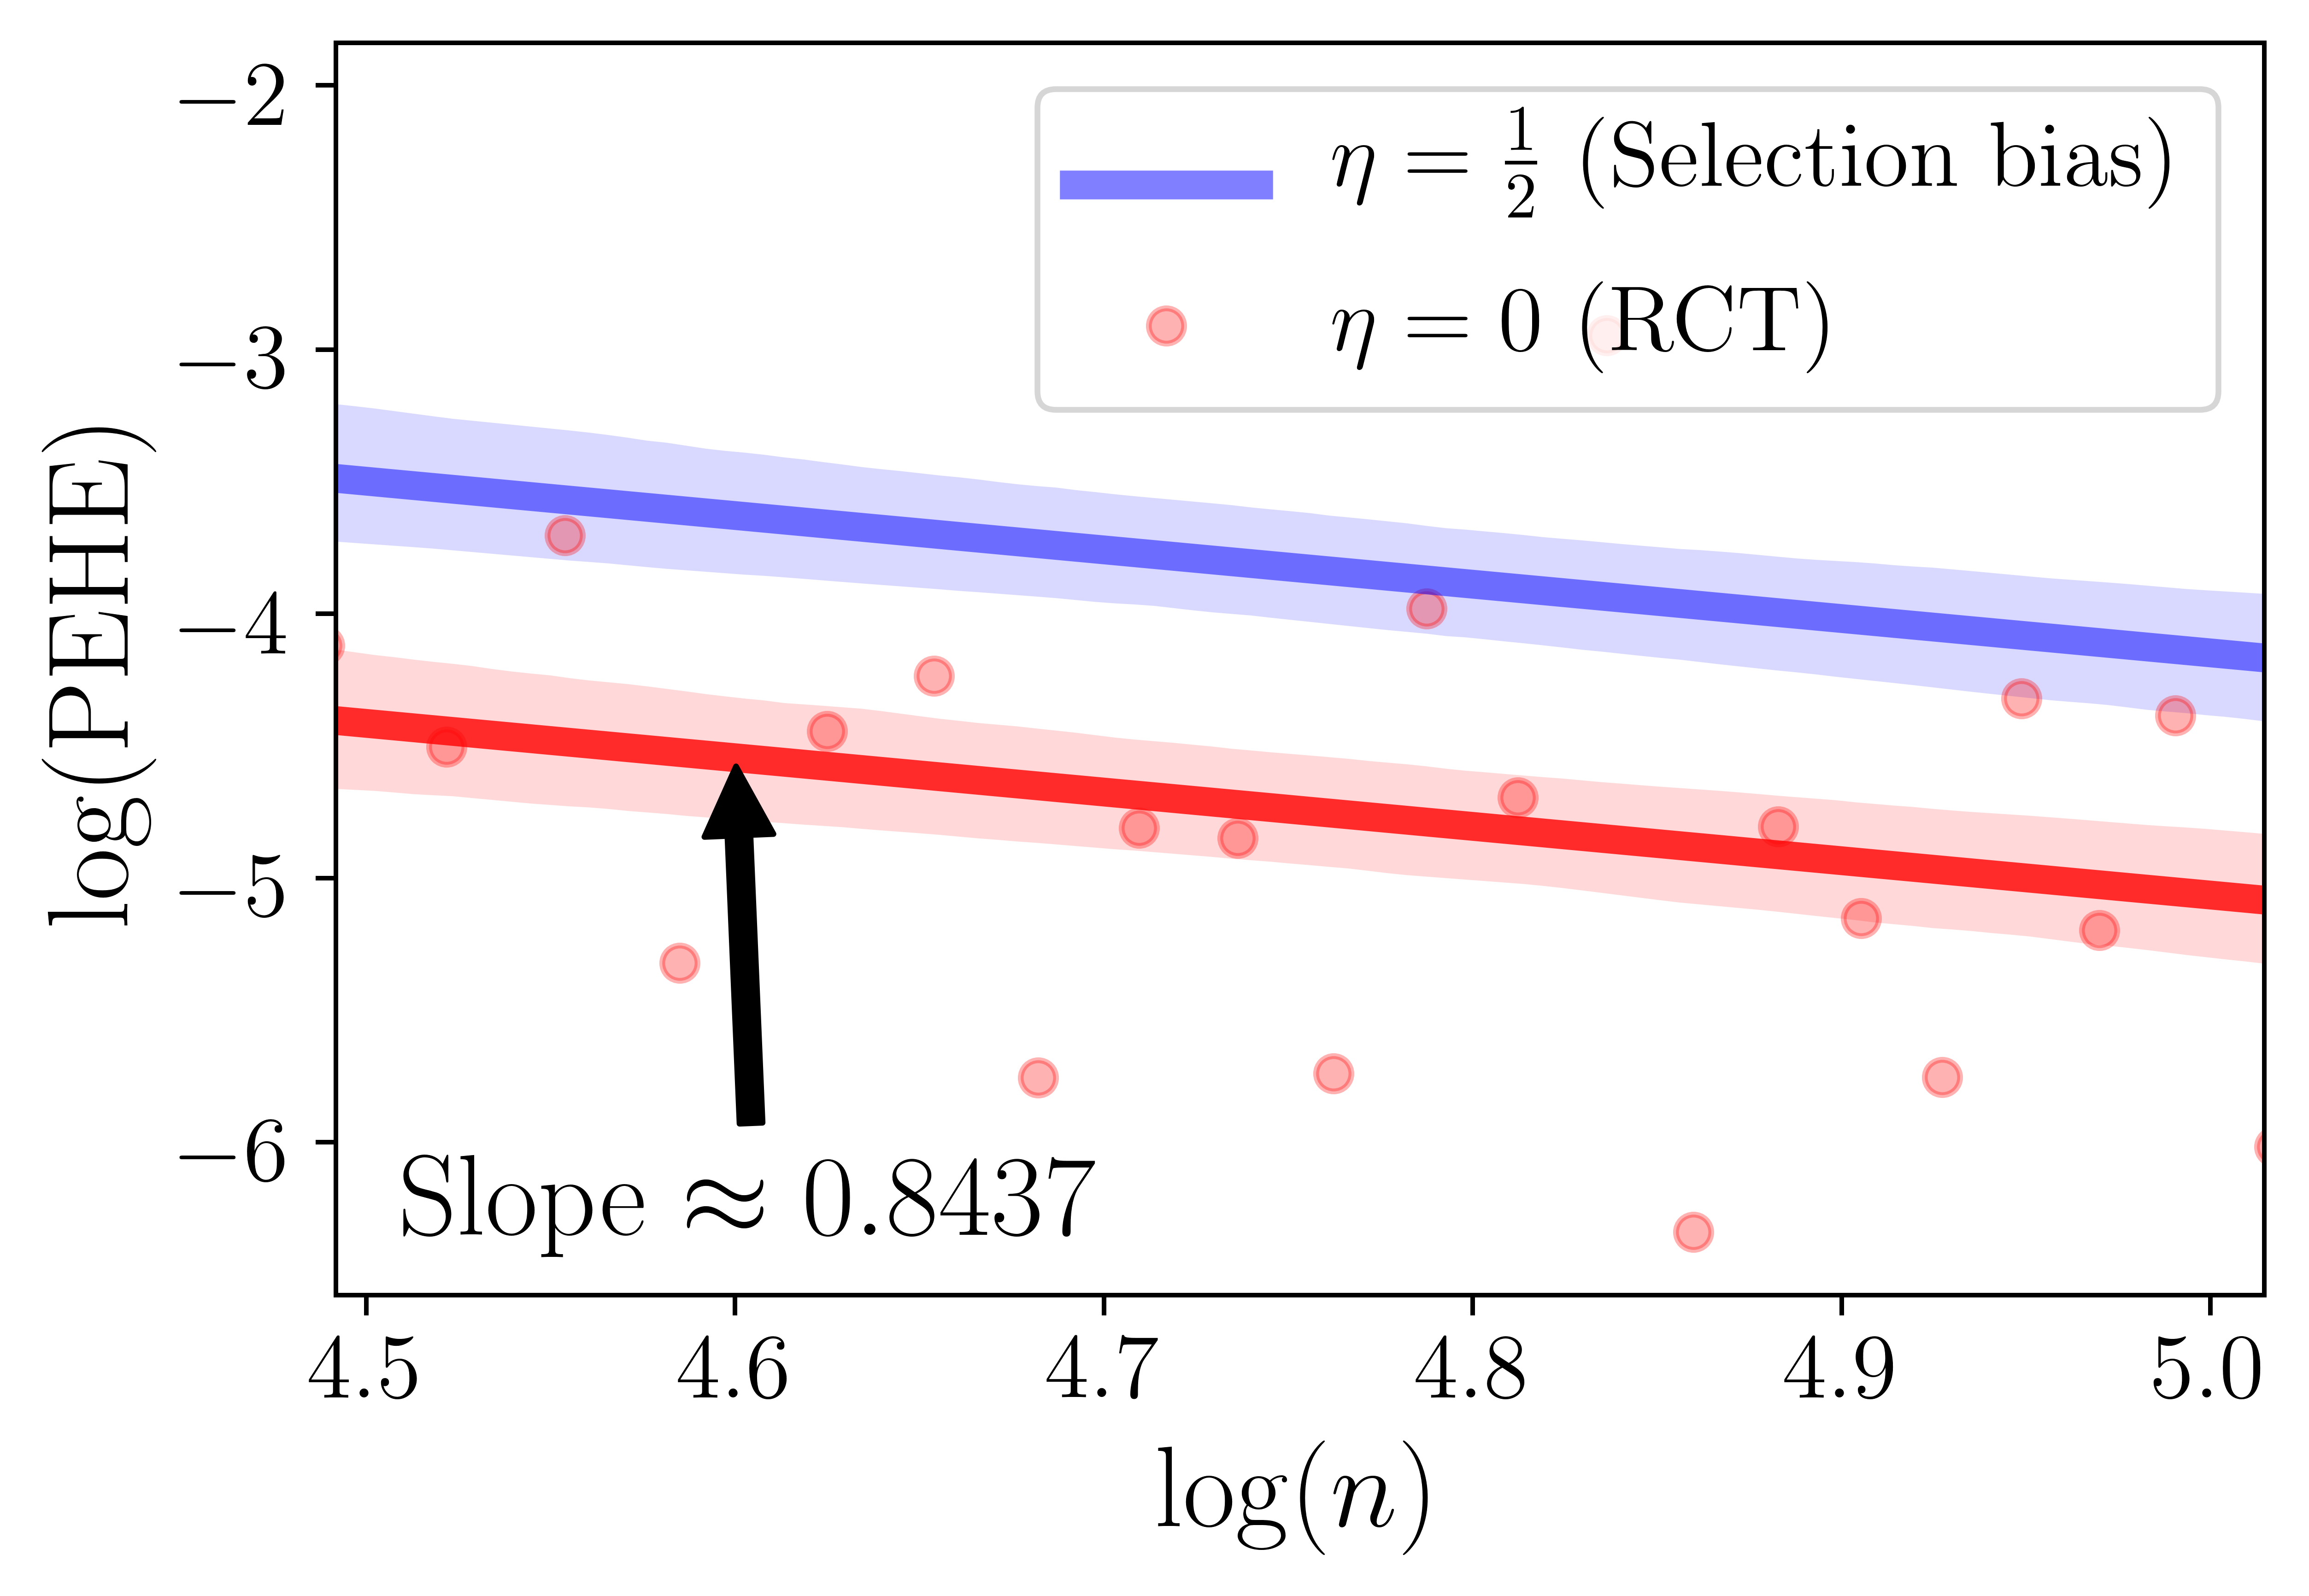
\includegraphics[width=0.9\linewidth]{ch2Fig2.png}
  \caption{\footnotesize Impact of selection bias.}
  \label{Ahmed1}
\end{subfigure}%
\begin{subfigure}{.33\textwidth}
  \centering
  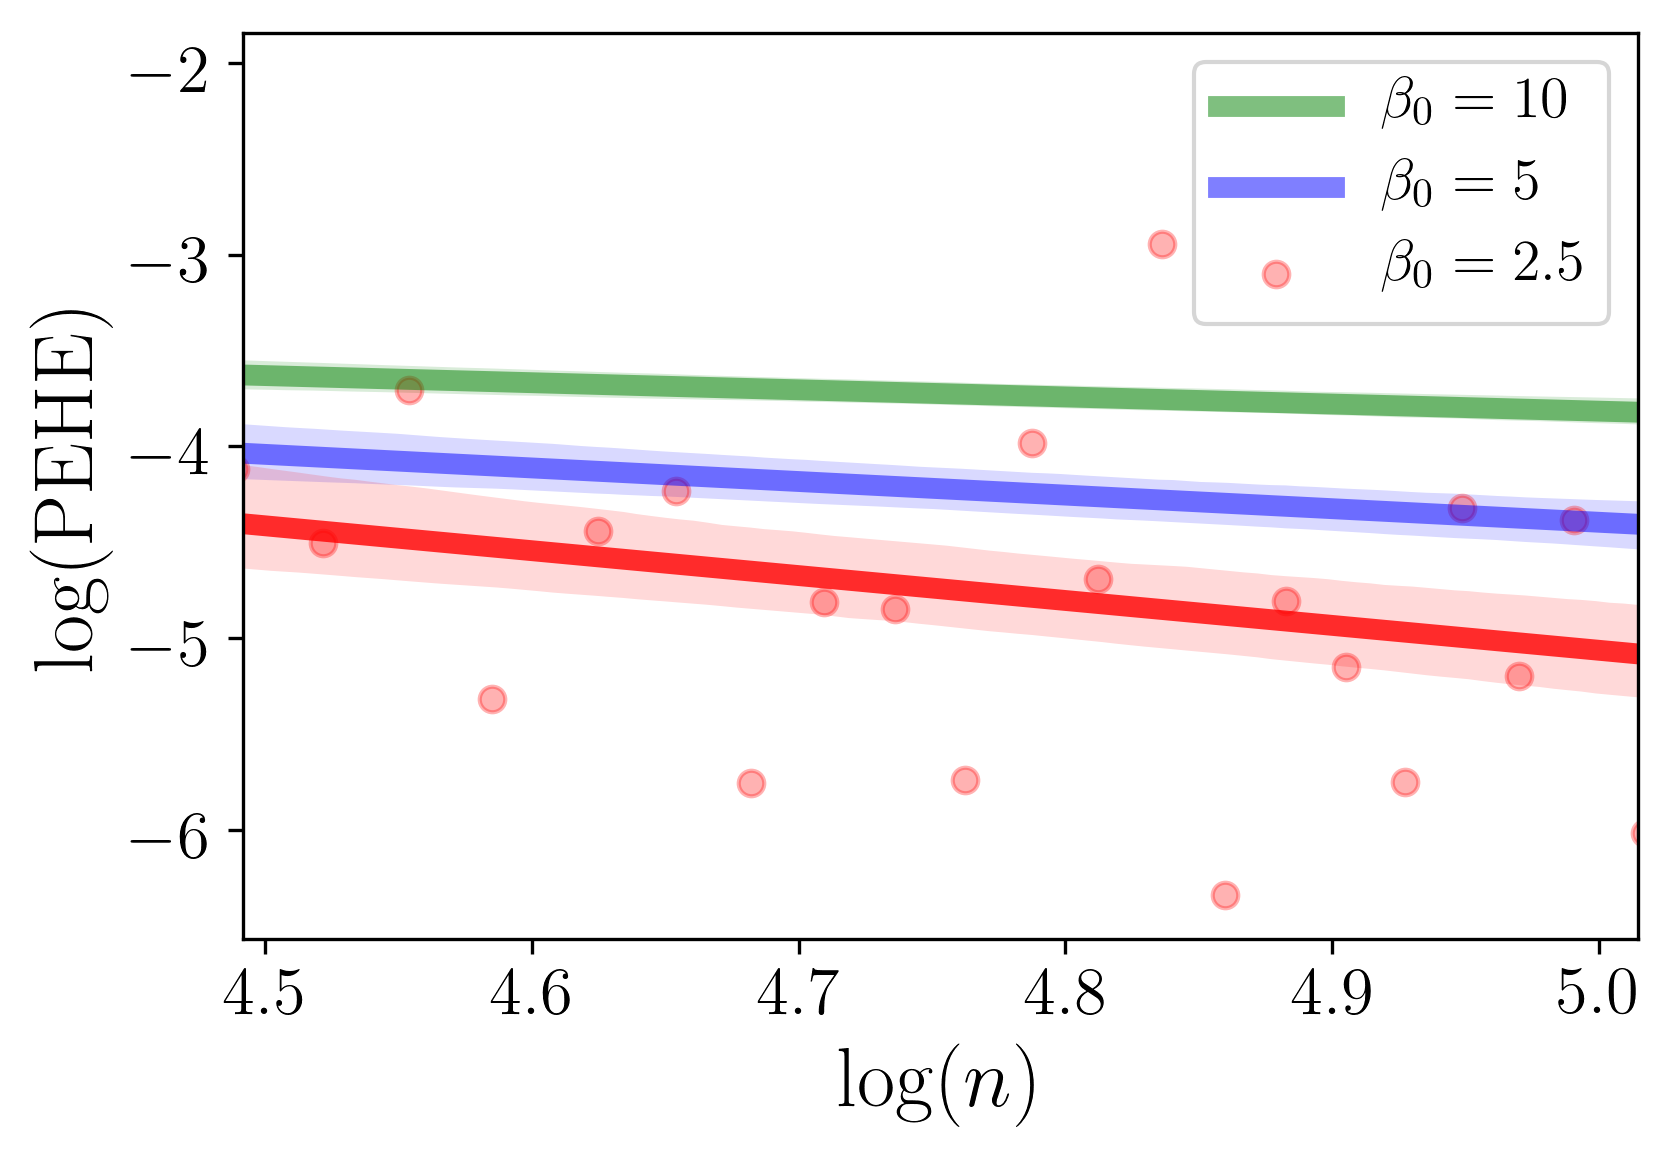
\includegraphics[width=0.9\linewidth]{ch2Fig3.png}
  \caption{\footnotesize Impact of over-smoothed priors.}
  \label{Ahmed2}
\end{subfigure}
\begin{subfigure}{.33\textwidth}
  \centering
  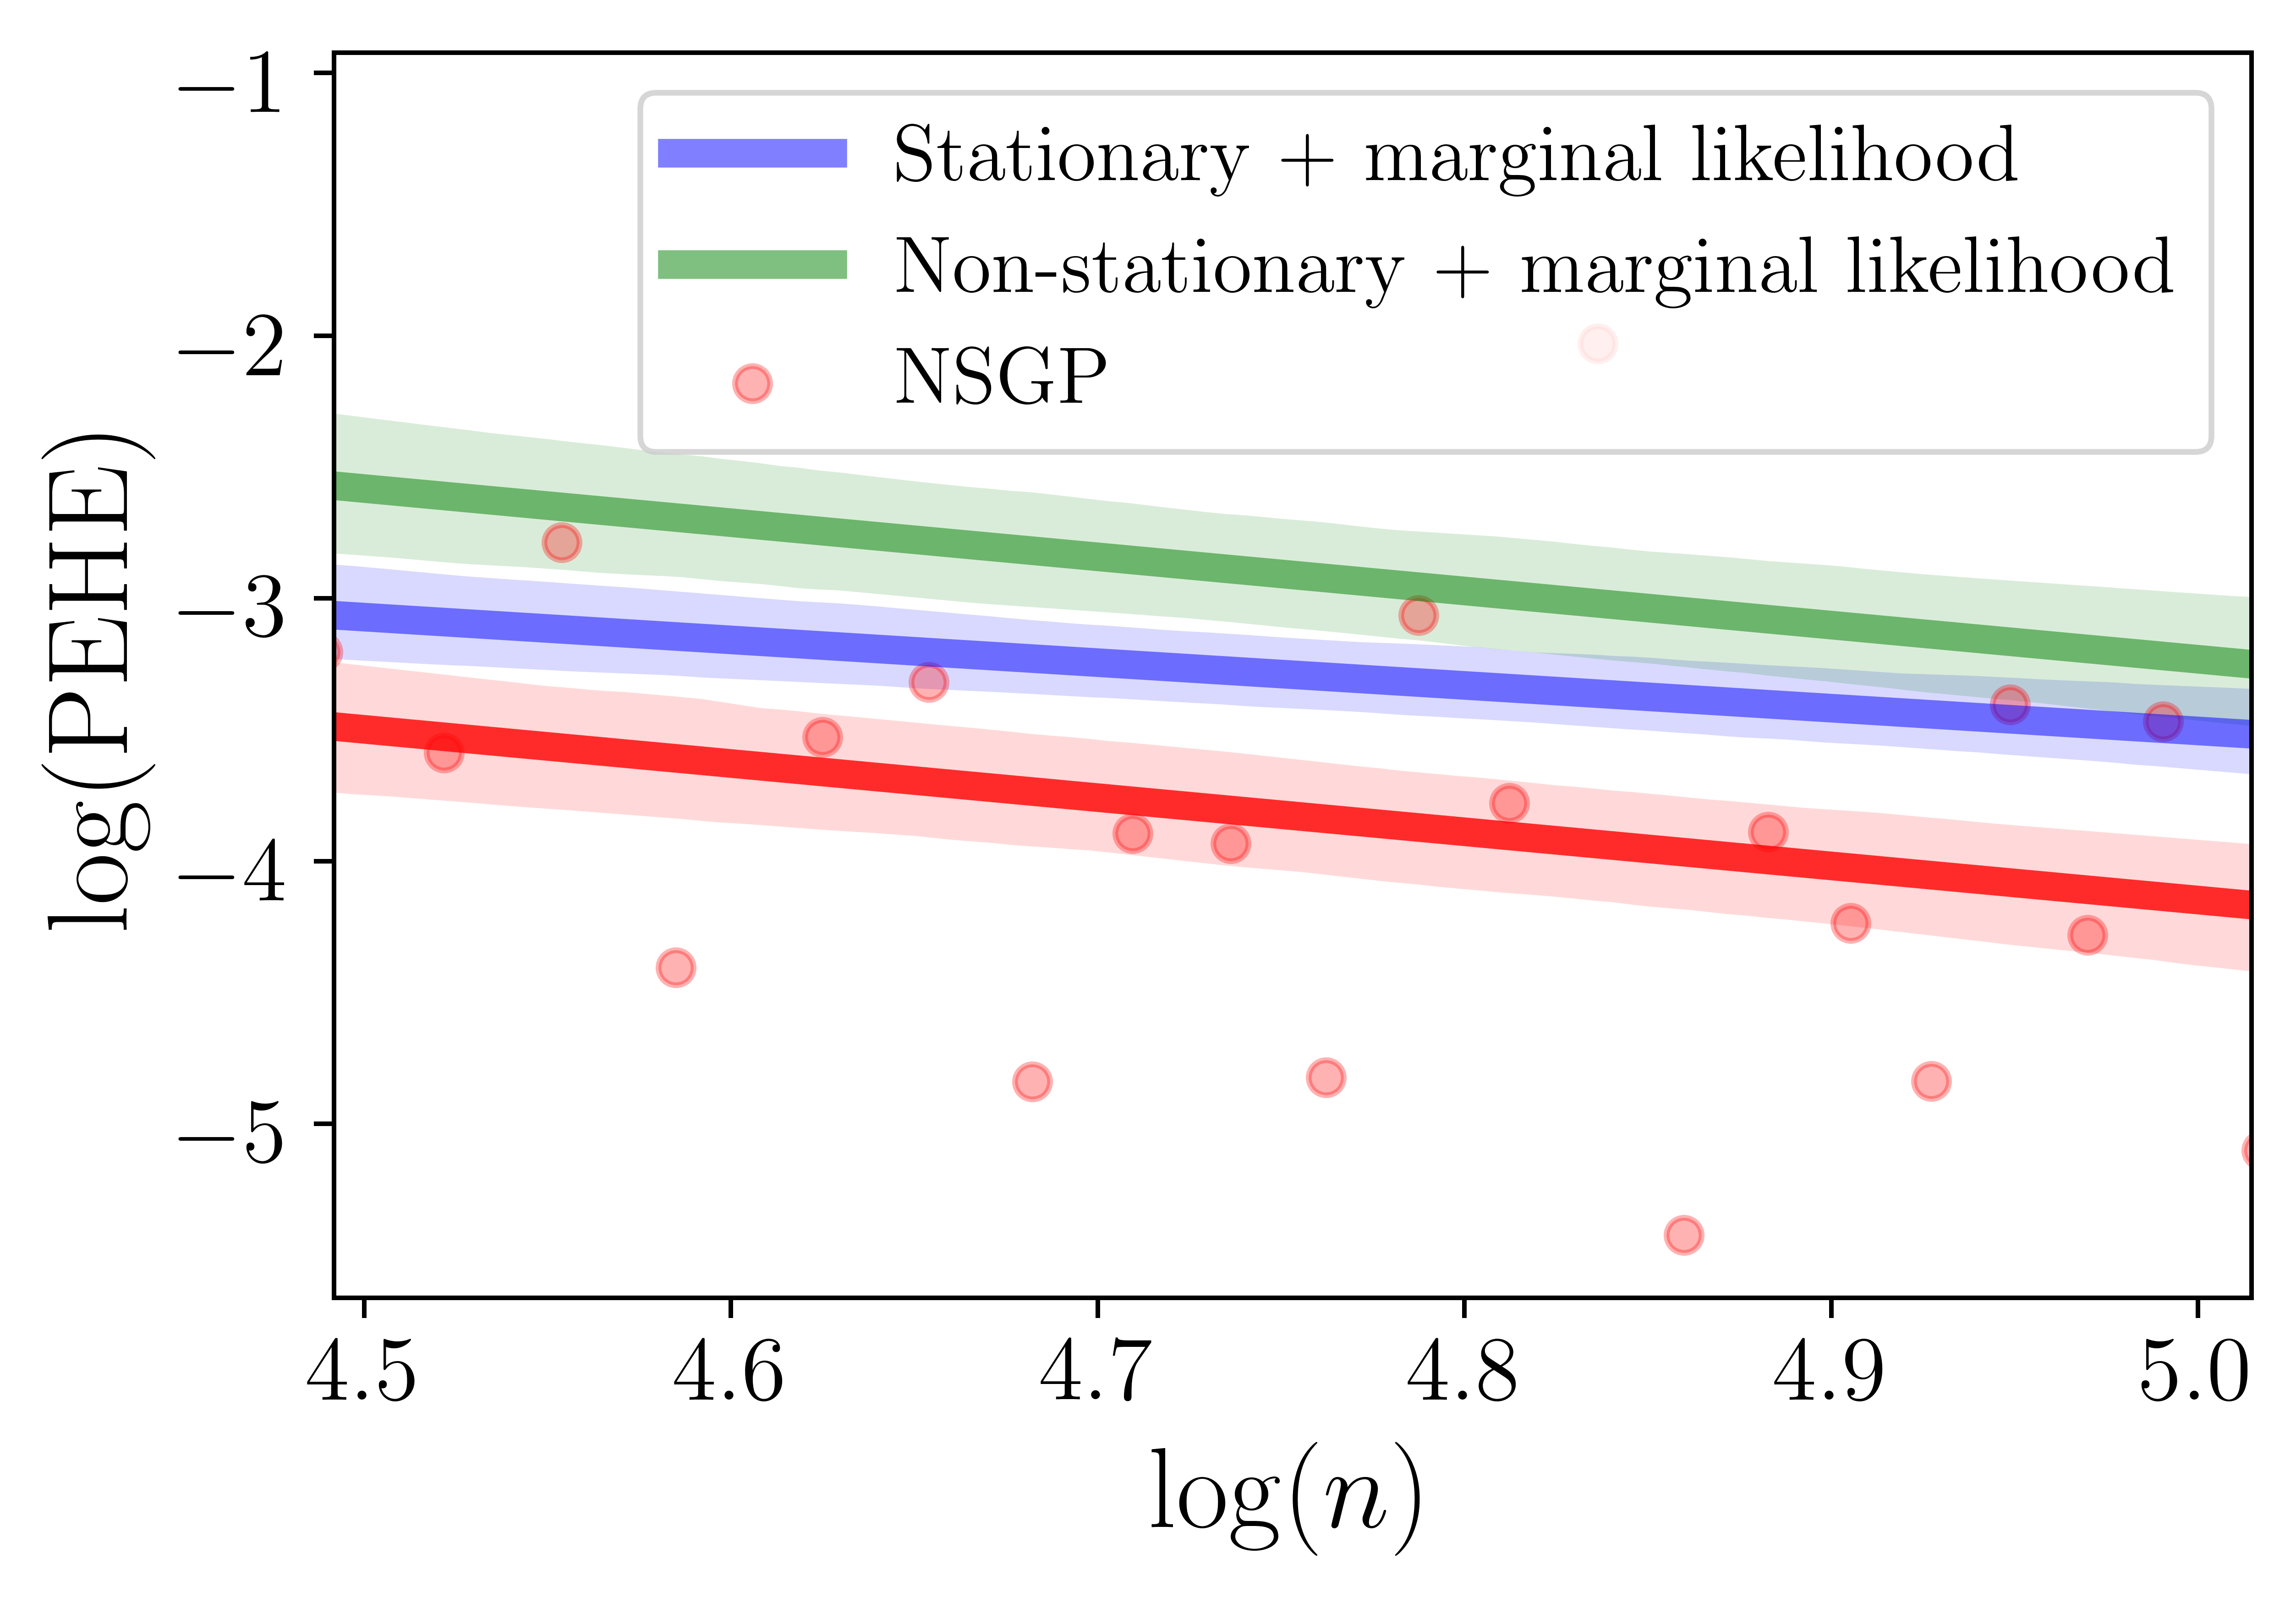
\includegraphics[width=0.9\linewidth]{ch2Fig4.png}
  \caption{\footnotesize Performance of different models.}
  \label{Ahmed3}
\end{subfigure}
	\caption{Scatter-plots and linear fits for the PEHE of NSGP on a $\log$-$\log$ scale in different simulation setups {(RCT: randomized controlled trial)}.}
	\label{ch2Fig2}
\end{figure*}

\section{Experiments}
In this Section, we check the validity of our analyses using a synthetic simulation setup (Subsection \ref{exp1}), and then evaluate the performance of our proposed model using data from a real-world clinical trial with simulated potential outcomes (Subsection \ref{exp2}). We will use the acronym \textbf{NSGP} to refer to the non-stationary GP model proposed in Section \ref{ch2sec4}.  
\subsection{Learning Brownian Response Surfaces}
\label{exp1}
\subsubsection{Synthetic Model}
\label{expexp0}
Let $\mathcal{X} = [0,1]$, and define a $\kappa$-fold integrated Brownian motion $B_{\kappa}$, $\kappa \in \mathbb{N}_+$, on $\mathcal{X}$ as follows:
\begin{align} 
B_{\kappa}(x) = \int_{0}^{x}\int_{0}^{x_\kappa} \cdots \int_{0}^{x_2} B_0(x_1) \,dx_1\, dx_2 \cdots dx_{x_\kappa}, \nonumber 
\end{align}
where $B_0(.)$ is a standard Brownian motion (Wiener process). Sample paths of $B_0$ are almost surely H\"older regular with exponent $\frac{1}{2}$ \cite{karatzas2012brownian}. Since $B_0(x)$ is almost surely non-differentiable everywhere in $\mathcal{X}$, then sample paths of $B_{\kappa}(x)$ are H\"older with exponent $\kappa + \frac{1}{2}$, i.e. $B_{\kappa} \in H^{\kappa+\frac{1}{2}}$ with probability 1. Therefore, when the true response surfaces are $\kappa$-fold integrated Brownian paths, the optimality and achievability results in Theorems 1 and 2 should hold. To this end, we simulate the true response surfaces $f_0 \in H^{\alpha_0}$ and $f_1 \in H^{\alpha_1}$ as $\boldsymbol{f_0 \sim B_{\alpha_0-\frac{1}{2}}}$, and $\boldsymbol{f_1 \sim B_{\alpha_1-\frac{1}{2}}}$, where we set $\boldsymbol{\alpha_0 = 2.5}$ and $\boldsymbol{\alpha_1 = 5.5}$. The propensity score is modeled as a parametrized logistic function $\boldsymbol{p(x\,|\,\eta) = (1+e^{-\eta\,(x-\frac{1}{2})})^{-1}}$, where $\eta \in \mathbb{R}$ is a parameter that determines the severity of selection bias. For a pair of fixed Brownian paths $f_0$ and $f_1$, synthetic observational samples $\boldsymbol{(X_i,W_i,Y^{\mbox{\tiny $(W_i)$}}_i)_i}$ are generated as follows: $\boldsymbol{X_i \sim \mbox{Uniform}[0,1]}$, $\boldsymbol{W_i \sim \mbox{Bernoulli}(p(x\,|\,\eta))}$, and $\boldsymbol{Y^{\mbox{\tiny $(W_i)$}}_i \sim f_{\mbox{\tiny $W_i$}} + \mathcal{N}(0,\sigma^2)}$, where $\boldsymbol{\sigma^2 = 0.1}$. 

\begin{table*}[t]
\centering
%\begin{tcolorbox}[tab3,tabularx={cc|l||c|c|cc|l||c|c}] 
\begin{tabular}{|cc|l||c|c|cc|l||c|c|}
\hline
\textbf{\tiny [Q1]} & \textbf{\tiny [Q2]} & \textbf{\tiny Model} & \textbf{\tiny In-sample $\sqrt{\mbox{PEHE}}$} & \textbf{\tiny Out-of-sample $\sqrt{\mbox{PEHE}}$} & \textbf{\tiny [Q1]} & \textbf{\tiny [Q2]} & \textbf{\tiny Model} & \textbf{\tiny In-sample $\sqrt{\mbox{PEHE}}$} & \textbf{\tiny Out-of-sample $\sqrt{\mbox{PEHE}}$} \\ \hline \hline
\mbox{\footnotesize $\boldsymbol{\checkmark}$} & \mbox{\footnotesize $\boldsymbol{\checkmark}$} & \mbox{\tiny \textbf{NSGP}} & \mbox{\tiny 0.51 $\pm$ 0.013} & \mbox{\tiny 0.64 $\pm$ 0.030} & \mbox{\footnotesize $\boldsymbol{\checkmark}$} & & \mbox{\tiny T-XGBoost} & \mbox{\tiny 1.46 $\pm$ 0.081} & \mbox{\tiny 1.98 $\pm$ 0.152} \\
& & \mbox{\tiny SGP} & \mbox{\tiny 0.95 $\pm$ 0.021} & \mbox{\tiny 1.21 $\pm$ 0.052} & & & \mbox{\tiny S-XGBoost} & \mbox{\tiny 2.97 $\pm$ 0.211} & \mbox{\tiny 3.04 $\pm$ 0.216} \\
\mbox{\footnotesize $\boldsymbol{\checkmark}$} & \mbox{\footnotesize $\boldsymbol{\checkmark}$} & \mbox{\tiny CMGP} & \mbox{\tiny 0.61 $\pm$ 0.011} & \mbox{\tiny 0.76 $\pm$ 0.012} & \mbox{\footnotesize $\boldsymbol{\checkmark}$} & & \mbox{\tiny T-AdaBoost} & \mbox{\tiny 2.40 $\pm$ 0.177} & \mbox{\tiny 2.79 $\pm$ 0.212} \\
\mbox{\footnotesize $\boldsymbol{\checkmark}$} & & \mbox{\tiny TARNet} & \mbox{\tiny 0.88 $\pm$ 0.021} & \mbox{\tiny 0.95 $\pm$ 0.025} & & & \mbox{\tiny S-AdaBoost} & \mbox{\tiny 4.53 $\pm$ 0.317} & \mbox{\tiny 4.56 $\pm$ 0.312} \\
 & \mbox{\footnotesize $\boldsymbol{\checkmark}$} & \mbox{\tiny BNN} & \mbox{\tiny 2.21 $\pm$ 0.115} & \mbox{\tiny 2.15 $\pm$ 0.125} & \mbox{\footnotesize $\boldsymbol{\checkmark}$} & & \mbox{\tiny T-OLS} & \mbox{\tiny 1.85 $\pm$ 0.107} & \mbox{\tiny 1.94 $\pm$ 0.122} \\
\mbox{\footnotesize $\boldsymbol{\checkmark}$} & \mbox{\footnotesize $\boldsymbol{\checkmark}$} & \mbox{\tiny CFR Wass.} & \mbox{\tiny 0.71 $\pm$ 0.018} & \mbox{\tiny 0.76 $\pm$ 0.032} & & & \mbox{\tiny S-OLS} & \mbox{\tiny 5.06 $\pm$ 0.357} & \mbox{\tiny 5.05 $\pm$ 0.352} \\
\mbox{\footnotesize $\boldsymbol{\checkmark}$} & \mbox{\footnotesize $\boldsymbol{\checkmark}$} & \mbox{\tiny CFR MMD} & \mbox{\tiny 0.73 $\pm$ 0.021} & \mbox{\tiny 0.78 $\pm$ 0.022} & \mbox{\footnotesize $\boldsymbol{\checkmark}$} & & \mbox{\tiny T-DNN} & \mbox{\tiny 3.36 $\pm$ 0.137} & \mbox{\tiny 3.46 $\pm$ 0.142} \\
\mbox{\footnotesize $\boldsymbol{\checkmark}$} & & \mbox{\tiny T-Random Forest} & \mbox{\tiny 1.41 $\pm$ 0.071} & \mbox{\tiny 2.21 $\pm$ 0.162} & & & \mbox{\tiny S-DNN} & \mbox{\tiny 3.56 $\pm$ 0.217} & \mbox{\tiny 3.64 $\pm$ 0.212} \\
& & \mbox{\tiny S-Random Forest} & \mbox{\tiny 2.72 $\pm$ 0.241} & \mbox{\tiny 2.91 $\pm$ 0.252} & & \mbox{\footnotesize $\boldsymbol{\checkmark}$} & \mbox{\tiny MARS} & \mbox{\tiny 1.66 $\pm$ 0.106} & \mbox{\tiny 1.74 $\pm$ 0.112} \\
 & \mbox{\footnotesize $\checkmark$} & \mbox{\tiny Causal Forest} & \mbox{\tiny 2.41 $\pm$ 0.141} & \mbox{\tiny 2.82 $\pm$ 0.181} & & & \mbox{\tiny $k$-NN} & \mbox{\tiny 2.69 $\pm$ 0.177} & \mbox{\tiny 4.06 $\pm$ 0.212} \\
& & \mbox{\tiny BART} & \mbox{\tiny 2.00 $\pm$ 0.141} & \mbox{\tiny 2.22 $\pm$ 0.151} & & \mbox{\footnotesize $\boldsymbol{\checkmark}$} & \mbox{\tiny PSM} & \mbox{\tiny 4.92 $\pm$ 0.312} & \mbox{\tiny 4.92 $\pm$ 0.312} \\
& \mbox{\footnotesize $\boldsymbol{\checkmark}$} & \mbox{\tiny BCF} & \mbox{\tiny 1.31 $\pm$ 0.061} & \mbox{\tiny 1.71 $\pm$ 0.102} & & \mbox{\footnotesize $\boldsymbol{\checkmark}$} & \mbox{\tiny TMLE} & \mbox{\tiny 5.27 $\pm$ 0.357} & \mbox{\tiny 5.27 $\pm$ 0.352} \\
\hline
%\end{tcolorbox}
\end{tabular}
\caption{Simulation results for the IHDP dataset. The values reported correspond to the average PEHE (\mbox{\footnotesize $\pm$ 95$\%$ confidence intervals}).}
\label{TableCh1}
\end{table*}


\subsubsection{Experiments and Results}  
\label{expexp}
Using the setup in Section \ref{expexp0}, we conducted the following Monte Carlo simulations to verify our theoretical findings and highlight the merits of our NSGP model. 	

\textbf{$\bullet$ \textit{Verifying Theorems 1 and 2}:} In order to check the validity of the results of Theorems 1 and 2, we use a NSGP Mat\'ern prior $\mathcal{GP}(0,\boldsymbol{K}_{\beta})$, with length-scale parameters $\beta_0$ and $\beta_1$ that are matched exactly with the regularities of the Brownian paths $f_0$ and $f_1$ (i.e., $\beta_0 = 2.5$ and $\beta_1 = 5.5$). According to Theorem 1, the optimal rate for estimating the CATE $T = f_1 - f_0$ is $n^{\frac{-5}{6}}$, and from Theorem 2, the NSGP with $\beta_0 = 2.5$ and $\beta_1 = 5.5$ should achieve that rate. 

Figure \ref{ch2Fig2} provides a scatter-plot for the PEHE achieved by the NSGP with respect to the number of samples on a $\log$-$\log$ scale for different settings of $\eta$. We fit a linear regression model that describes the PEHE behavior in the $\log$-$\log$ scale. We found the slope of the linear fit to be 0.8437, which is very close\footnote{The minor discrepancy is a result of the residual error in the linear regression fit.} to the slope of $\frac{5}{6} \approx 0.833$ predicted by Theorem 1. Moreover, by changing the magnitude of $\eta$ from $0$ to $\frac{1}{2}$, the PEHE curve did not exhibit any significant change in its slope, and was only moved upwards by a constant offset. On the contrary, Figure \ref{ch2Fig2} shows the PEHE behavior when the NSGP prior is over-smoothed ($\beta_0 > \alpha_0$) for $\eta=0$: as predicted by Theorem 2, learning becomes sluggish (slopes become less steep) as $\beta_0$ increase since the matching condition in (\ref{ch2eq11}) does not hold any more.     

\textbf{$\bullet$ \textit{NSGPs do not leave any money on the table:}} In this experiment, we show that the different components of the NSGP model allow it to perform well in small and large sample regimes. We set a strong selection bias of $\eta = \frac{1}{2}$ and compare the $\log(\mbox{PEHE})$ characteristic of NSGP with a model that uses the same non-stationary kernel as NSGP, and another model that uses a standard stationary kernel, but both models are tuned using marginal likelihood maximization. As we can see in Figure \ref{ch2Fig2}, the model with the non-stationary kernel achieves the same learning rate as NSGP, but exhibits a large offset as it does not account for selection bias, whereas the stationary model fails to learn the smoothness of the rougher Brownian motion since it assigns the same length-scale to both surfaces, and hence it over-smooths the prior, achieving a suboptimal rate. 

\subsection{The Infant Health and Development Program}
\label{exp2}
We evaluated the performance of the NSGP model presented in Section \ref{ch2sec41} using the standard semi-synthetic experimental setup designed by Hill in \cite{hill2011bayesian}. We report a state-of-the-art result in this setup, and draw connections between our experimental results and our analyses.

\subsubsection{Data and Benchmarks}
\label{expexp0ZXC}  
The Infant Health and Development Program (IHDP) is an interventional program intended to enhance the health of premature infants \cite{hill2011bayesian}. \cite{hill2011bayesian} extracted features and treatment assignments from a real-world clinical trial, and introduced selection bias to the data artificially by removing a subset of the patients. The potential outcomes are simulated according to the standard non-linear "Response Surface B" setting in \cite{hill2011bayesian}. The dataset comprised 747 subjects, with 25 features for each subject. Our experimental setup is identical to \cite{hill2011bayesian,johansson2016learning,shalit2016estimating,alaa2017bayesian}: we run 1000 experiments in which we compute the in-sample and out-of-sample $\sqrt{\mbox{PEHE}}$ (with 80/20 training/testing splits), and report average results in Table \ref{TableCh1}. 

We compared the performance of NSGP with a total of 23 CATE estimation benchmarks. We considered: tree-based algorithms (BART \cite{hill2011bayesian}, Causal forests \cite{wager2017estimation}, Bayesian causal forests \cite{hahn2017bayesian}), methods based on deep learning (CFR Wass., CFR MMD, BNN, TARnet \cite{shalit2016estimating}), multivariate additive regression splines (MARS) \cite{powers2017some}, Gaussian processes (CMGP) \cite{alaa2017bayesian}, nearest neighbor matching ($k$-NN), propensity score matching (PSM), and targeted maximum likelihood (TMLE) \cite{porter2011relative}. We also composed a number of T-learners and S-learners as in \cite{kunzel2017meta}, using a variety of baseline machine learning algorithms (DNN stands for deep networks and OLS stands for linear regression). 

\subsubsection{Results and Conclusions}  
\label{expexpZZZ}
As we can see in Table \ref{TableCh1}, the proposed NSGP model significantly outperforms \textbf{all} competing benchmarks. The combined benefit of the two components of an NSGP (non-stationary kernel and doubly-robust hyperparameters) is highlighted by comparing its performance to a vanilla SGP (stationary GP) with marginal likelihood maximization. The gain with respect to such a model is a 2-fold improvement in the PEHE. 

Because the IHDP dataset has a ``moderate" sample size, both selection bias and learning rate seem to impact the performance. Thus, our method took advantage of having addressed modeling questions \textbf{[Q1]} and \textbf{[Q2]} appropriately by being both ``rate-optimal" and ``bias-aware". 

The check marks in columns \textbf{[Q1]} and \textbf{[Q2]} designate methods that address modeling questions \textbf{[Q1]} and \textbf{[Q2]} ``appropriately" in the light of the analysis presented in Section \ref{ch2sec3}. Methods with \textbf{[Q1]} checked use a regression structure with ``outcome-specific" hyperparameters, and methods with \textbf{[Q2]} checked adjust for selection bias. A general observation is that the structure of the regression model seem to matter much more than the strategy for handling selection bias. This is evident from the fact that the TARnet model (does not handle bias but models outcomes separately) significantly outperforms BNN (handles bias but uses a single-surface model \cite{shalit2016estimating}), and that all T-learners (models 2 separate response surfaces) outperformed their S-shaped counterparts (models a single surface). For parametric models, such as OLS, the issue of selecting the right regression structure is even more crucial. 

To sum up, the results in Table \ref{TableCh1} imply that selecting the right regression structure is crucial for rate-optimality in sufficiently large dataset, whereas handling selection bias provides an extra bonus. In Table \ref{TableCh1}, methods that address both \textbf{[Q1]} and \textbf{[Q2]} (NSGP, CMGP, and CFR. Wass and MMD) displayed a superior performance.

\chapter{Symbolic Approaches to Prognostic Model Interpretability}

The ability to interpret the predictions of a (predictive or causal) machine learning model brings about patient and clinician trust, and supports understanding of the underlying disease being modeled \cite{lundberg2017unified,lipton2016mythos, alaa2019}. In many clinical settings, interpretability can be a crucial requirement for the deployment of machine learning, since a model's predictions would inform critical decision-making. Model explanations can also be central in other domains, such as natural sciences \cite{schmidt2009distilling,wang2019symbolic}, where the primary utility of a model is to help understand an underlying phenomenon, rather than merely making predictions about it. Unfortunately, most state-of-the-art models --- such as ensemble~models, kernel methods, and neural networks --- are perceived as being complex ``black-boxes'', the predictions of which are too hard to be interpreted by human subjects \cite{lundberg2017unified,yoon2018invase,jordon2018knockoffgan,shrikumar2017learning,lou2013accurate,elenberg2017streaming,bouchard2017union,melis2018towards,tsang2018neural,zhang2018interpreting,chen2018learning,ribeiro2016should}. 

\begin{figure*}[t]
\centering
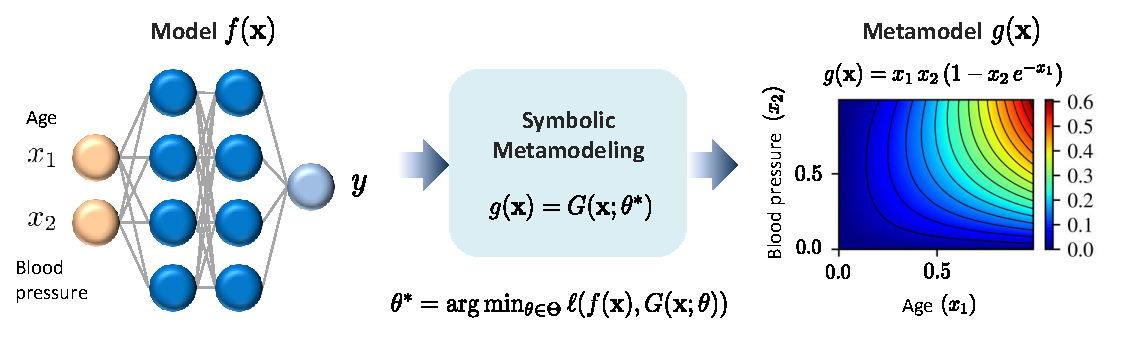
\includegraphics[width=6in]{ch3Fig1.pdf}
\caption{Pictorial depiction of the symbolic metamodeling framework. Here, the model $f(\boldsymbol{x})$ is a deep neural network (left), and the metamodel $g(\boldsymbol{x})$ is a closed-form expression $x_1\,x_2\,(1-x_2\,\exp(-x_1))$ (right).}
\label{ch3fig1} 
\end{figure*}

In this Chapter, we approach the problem of model interpretation by introducing the \textit{symbolic metamodeling} framework for expressing black-box models in terms of transparent mathematical equations that can be easily understood and analyzed by human subjects (Section \ref{ch3sec2}). The proposed metamodeling procedure takes as an input a (trained) model --- represented by a black-box function $f(\boldsymbol{x})$ that maps a feature $\boldsymbol{x}$ to a prediction $y$ --- and retrieves a \textit{symbolic metamodel} $g(\boldsymbol{x})$, which is meant to be an interpretable mathematical abstraction of $f(\boldsymbol{x})$. The metamodel $g(\boldsymbol{x})$ is a tractable symbolic expression comprising a finite number of familiar functions (e.g., polynomial, analytic, algebraic, or closed-form expressions) that are combined via elementary arithmetic operations (i.e., addition and multiplication), which makes it easily understood by inspection, and can be analytically manipulated via symbolic computation engines such as {\footnotesize \texttt{Mathematica}} \cite{abell2017mathematica}, {\footnotesize \texttt{Wolfram alpha}} \cite{wolfram2013wolfram}, or {\footnotesize \texttt{Sympy}} \cite{10.7717/peerj-cs.103}. Our approach is appropriate for models with small to moderate number of features, where the physical interpretation of these features are of primary interest. 

A high-level illustration of the proposed metamodeling approach is shown in Figure \ref{ch3fig1}. In this Figure, we consider an example of using a neural network to predict the risk of cardiovascular disease based on a (normalized) feature vector ${\bf x} = (x_1, x_2)$, where $x_1$ is a person's age and $x_2$ is their blood pressure. For a clinician using this model in their daily practice or in the context of an epidemiological study, the model $f({\bf x})$ is completely obscure --- it is hard to explain or draw insights into the model's predictions, even with a background knowledge of neural networks. On the other hand, the metamodel $g({\bf x}) = x_1\,x_2\,(1-x_2\exp(-x_1))$ is a fully transparent abstraction of the neural network model, from which one can derive explanations for the model's predictions through simple analytic manipulation, without the need to know anything about the model structure and its inner workings\footnote{Note that here we are concerned with explaining the predictions of a trained model, i.e., its \textit{response surface}. Other works, such as \cite{koh2017understanding}, focus on explaining the model's \textit{loss surface} in order to understand how it learns.}. Having such an explicit (simulatable) equation for predicting risks is already required by various clinical guidelines to ensure the transparency of prognostic models \cite{kattan2016american}. 

In order to find the symbolic metamodel $g({\bf x})$ that best approximates the original model $f({\bf x})$, we need to search a space of mathematical expressions and find the expression that minimizes a ``metamodeling loss'' $\ell(g({\bf x}), f({\bf x}))$. But how can we construct a space of symbolic expressions without predetermining its functional from? In other words, how do we know that the metamodel $g({\bf x}) = x_1\,x_2\,(1-x_2\exp(-x_1))$ in Figure \ref{ch3fig1} takes on an exponential form and not, say, a trigonometric or a polynomial functional form?   

To answer this question, we introduce a novel parameterized representation of symbolic expressions (Section \ref{ch3sec3}), $G({\bf x};\theta)$, which reduces to most familiar functional forms --- e.g., arithmetic, polynomial, algebraic, closed-form, and	analytic expressions, in addition to special functions, such as Bessel functions and Hypergeometric functions --- for different settings of a real-valued parameter $\theta$. The representation $G({\bf x};\theta)$ is based on Meijer $G$-functions \cite{meijer1946gfunc,meijer1936uber,beals2013meijer}, a class of contour integrals used in the mathematics community to find closed-form solutions for otherwise intractable integrals. The proposed Meijer $G$-function parameterization enables minimizing the metamodeling loss efficiently via gradient descent --- this is a major departure from existing approaches to {\it symbolic regression}, which use genetic programming to select among symbolic expressions that comprise a small number of predetermined functional forms \cite{orzechowski2018we,menezes2014symbolic,vladislavleva2009order}. 

Existing methods for model interpretation focus on crafting explanation models that support only one ``mode'' of model interpretation. For instance, methods such as DeepLIFT \cite{shrikumar2017learning} and LIME \cite{ribeiro2016should}, can explain the predictions of a model in terms of the contributions of individual features to the prediction, but cannot tell us whether the model is nonlinear, or whether statistical interactions between features exist. Other methods such as GA$^2$M \cite{lou2013accurate} and NIT \cite{tsang2018neural}, focus exclusively on uncovering the statistical interactions captured by the model, which may not be the most relevant mode of explanation in many application domains. Moreover, none of the existing methods can uncover the functional forms by which a model captures nonlinearities in the data --- such type of interpretation is important in applications such as applied physics and material sciences, since researchers in these fields focus on distilling an analytic law that describes how the model fits experimental data \cite{schmidt2009distilling,wang2019symbolic}.  

Our perspective on model interpretation departs from previous works in that, a symbolic metamodel $g({\bf x})$ is not hardwired to provide any specific type of explanation, but is rather designed to provide a full mathematical description of the original model $f({\bf x})$. In this sense, symbolic metamodeling should be understood as a tabula rasa upon which different forms of explanations can be derived --- as we will show in Section \ref{ch3sec4}, most forms of model explanation covered in previous literature can be arrived at through simple analytic manipulation of a symbolic metamodel. 

\begin{figure*}[t]
\centering
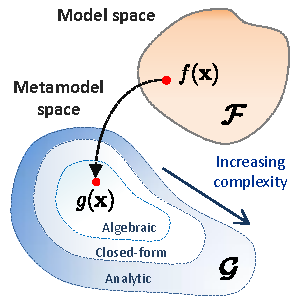
\includegraphics[width=2.5in]{ch3Fig2.pdf}
\caption{The metamodeling problem.}
\label{ch3fig2} 
\end{figure*}

\section{Symbolic Metamodeling}
\label{ch3sec2}
Let $f:\mathcal{X} \to \mathcal{Y}$ be a machine learning model trained to predict a target outcome $y \in \mathcal{Y}$ on the basis of a $d$-dimensional feature instance ${\bf x} = (x_{1},\ldots,x_{d}) \in \mathcal{X}$. We assume that $f(.)$ is a {\it black-box} model to which we only have query access, i.e., we can evaluate the model's output $y = f({\bf x})$ for any given feature instance ${\bf x}$, but we do not know the model's internal structure. Without loss of generality, we assume that the feature space $\mathcal{X}$ is the unit hypercube, i.e., $\mathcal{X} = [0,1]^d$.\\
\\
{\bf The metamodeling problem.} A {\it symbolic metamodel} $g \in \mathcal{G}$ is a ``model of the model'' $f$ that approximates $f({\bf x})$ for all ${\bf x} \in \mathcal{X}$, where $\mathcal{G}$ is a class of succinct mathematical expressions that are understandable to users and can be analytically manipulated. Typically, $\mathcal{G}$ would be set as the class of all arithmetic, polynomial, algebraic, closed-form, or analytic expressions. Choice of $\mathcal{G}$ will depend on the desired complexity of the metamodel. In most medical applications, we might opt to restrict $\mathcal{G}$ to algebraic expressions. Given $\mathcal{G}$, the metamodeling problem consists in finding the function $g$ in $\mathcal{G}$ that bests approximates the model $f$.

Figure \ref{ch3fig2} shows a pictorial depiction of the metamodeling problem as a mapping from the {\it modeling space} $\mathcal{F}$ --- i.e., the function class that the model $f$ inhabits\footnote{For instance, for an $L$-layer neural network, $\mathcal{F}$ is the space of compositions of $L$ nested activation functions. For a random forest with $L$ trees, $\mathcal{F}$ is the space of summations of $L$ piece-wise functions.} --- to the interpretable metamodeling space $\mathcal{G}$. Metamodling is only relevant when $\mathcal{F}$ spans functions that are considered uninterpretable to users. For models that are deemed interpretable, such as linear regression, $\mathcal{F}$ will already coincide with $\mathcal{G}$, because the linear model is already an algebraic expression (and a first-order polynomial). In this case, the best metamodel for $f$ is the model $f$ itself, i.e., $g = f$.

Formally, metamodeling can be formulated through the following optimization problem:  
\begin{align}
g^* = \arg \min_{g \in \mathcal{G}} \ell(g, f),\,\,\,\,\,\, \ell(g, f) = \|\,f\, - \,g\,\|_2^2 = \int_{\mathcal{X}} (g({\bf x}) - f({\bf x}))^2\, d{\bf x},
\label{ch3eq1}
\end{align}
where $\ell(.)$ is the {\it metamodeling loss}, which we set to be the mean squared error (MSE) between $f$ and $g$. In the following Section, we will focus on solving the optimization problem in (\ref{ch3eq1}).

\section{Metamodeling via Meijer $G$-functions}
\label{ch3sec3}
In order to solve the optimization problem in (\ref{ch3eq1}), we need to induce some structure into the metamodeling space $\mathcal{G}$. This is obviously very challenging since $\mathcal{G}$ encompasses infinitely many possible mathematical expressions with very diverse functional forms. For instance, consider the exemplary metamodel in Figure \ref{ch3fig1}, where $g({\bf x}) = x_1\,x_2\,(1-x_2\exp(-x_1))$. If $\mathcal{G}$ is set to be the space of all closed-form expressions, then it would include all polynomial, hyperbolic, trigonometric, logarithmic functions, rational and irrational exponents, and any combination thereof \cite{chow1999closed,borwein2013closed}. Expressions such as $g^{\prime}({\bf x}) = (x^2_1 + x^2_2)$ and $g^{\prime\prime}({\bf x}) = \sin(x_1)\cdot \cos(x_2)$ are both valid metamodels, i.e., $g^{\prime}, g^{\prime\prime} \in \mathcal{G}$, yet they each have functional forms that are very different from $g$. Thus, we need to parameterize $\mathcal{G}$ in such a way that it encodes all such functional forms, and enables an efficient solution to (\ref{ch3eq1}). 

To this end, we envision a parameterized metamodel $g({\bf x}) = G({\bf x};\theta),\, \theta \in \Theta$, where $\Theta = \mathbb{R}^M$ is a parameter space that fully specifies the metamodeling space $\mathcal{G}$, i.e., $\mathcal{G} = \{G(.;\theta): \theta \in \Theta\}$. Such parameterization should let $G({\bf x};\theta)$ reduce to different functions for different settings of $\theta$ --- for the aforementioned example, we should have $G({\bf x};\theta^{\prime}) = (x^2_1 + x^2_2)$ and $G({\bf x};\theta^{\prime\prime}) = \sin(x_1)\cdot \cos(x_2)$ for some $\theta^{\prime}, \theta^{\prime\prime} \in \Theta$. Given the parameterization $G({\bf x};\theta)$, the problem in (\ref{ch3eq1}) reduces to  
\begin{align}
g^*({\bf x}) = G({\bf x};\theta^*),\,\,\mbox{where}\,\, \theta^* = \arg \min_{\theta \in \Theta}\,\, \ell(G({\bf x};\theta), f({\bf x})).
\label{ch3eq2}
\end{align}
Thus, if we have a parameterized symbolic expression $G({\bf x};\theta)$, then metamodeling boils down to a straightforward parameter optimization problem. We construct $G({\bf x};\theta)$ in Section \ref{ch3Sec31}.

\subsection{Parameterizing symbolic metamodels with Meijer $G$-functions}
\label{ch3Sec31}
We propose a parameterization of $G({\bf x};\theta)$ that includes two steps. The first step involves decomposing $G({\bf x};\theta)$ into a combination of univariate functions. The second step involves modeling these univariate functions through a very general class of special functions that includes most known familiar functions as particular cases. Both steps are explained in detail in what follows. \\   
\\
{\bf Step 1: Decomposing the metamodel.} We breakdown the {\it multivariate} function $g({\bf x})$ into simpler, {\it univariate} functions. From the {\it Kolmogorov superposition theorem} \cite{kolmogorov1957representation}, we know that every multivariate continuous function $g({\bf x})$ can be written as a finite composition of univariate continuous functions and the addition operation as follows\footnote{The Kolmogorov decomposition in (\ref{ch3eq3}) is a universal function approximator \cite{hornik1989multilayer}. In fact, (\ref{ch3eq3}) can be thought of as a 2-layer neural network with generalized activation functions \cite{kuurkova1992kolmogorov, girosi1989representation, igelnik2003kolmogorov, hornik1989multilayer, cybenko1989approximation}.}:  
\begin{equation}
g(\mathbf{x}) = g(x_{1},\ldots,x_{n}) = \sum_{i=0}^{r}g^{out}_{i}\left(\,\sum_{j=1}^{d}g^{in}_{ij}(x_{j})\,\right),
\label{ch3eq3}
\end{equation}
where $\mbox{\footnotesize $g_i^{in}$}$ and $\mbox{\footnotesize $g_{ij}^{out}$}$ are continuous univariate {\it basis functions}, and $r \in \mathbb{N}_+$. The exact decomposition in (\ref{ch3eq3}) always exists for $r = 2d$, and for some basis functions $\mbox{\footnotesize $g_i^{out}: \mathbb{R} \to \mathbb{R}$}$, and $\mbox{\footnotesize $g_{ij}^{in}: [0,1] \to \mathbb{R}$}$ \cite{sprecher1993universal}. When $r=1$, (\ref{ch3eq3}) reduces to the generalized additive model \cite{hastie2017generalized}. While we proceed our analysis with the general formula in (\ref{ch3eq3}), in our implementation we set $r=1$, $g^{out}$ as the identify function, and include extra functions $g^{in}_{ij}$ of the interactions $\{x_i\,x_j\}_{i,j}$ to account for the complexity of $g(\mathbf{x})$.\\
\\ 
{\bf Step 2: Meijer $G$-functions as basis functions.} Based on the decomposition in (\ref{ch3eq3}), we can now parameterize metamodels in terms of their univariate bases, i.e., $\mbox{\footnotesize $G({\bf x};\theta) = G({\bf x};\{g^{out}_{i}\}_i, \{g^{in}_{ij}\}_{i,j})$}$, where every selection of a different set of bases would lead to a different corresponding metamodel. However, in order to fully specify the parameterization $\mbox{\footnotesize $G({\bf x};\theta)$}$, we still need to parameterize the basis functions themselves in terms of real-valued parameters that we can practically optimize, while ensuring that the corresponding parameter space spans a wide range of symbolic expressions. 

To specify $G({\bf x};\theta)$, we model the basis functions in (\ref{ch3eq3}) as instances of a Meijer $G$-function --- a {\it univariate} special function given by the following line integral in the complex plane $s$ \cite{meijer1946gfunc, meijer1936uber}:\\ 
\begin{equation}
\MeijerG{m}{n}{p}{q}{a_1,\ldots,a_p}{b_1,\ldots,b_q}{x} = \frac{1}{2\pi i} \int_\mathcal{L} \frac{\prod^m_{j=1} \Gamma(b_j - s)\,\prod^n_{j=1} \Gamma(1 - a_j + s)}{\prod^q_{j=m+1} \Gamma(1 - b_j + s)\,\prod^p_{j=n+1} \Gamma(a_j + s)} \,\, x^s \, ds,
\label{ch3eq4}
\end{equation}\\
where $\Gamma(.)$ is the Gamma function and $\mathcal{L}$ is the integration path in the complex plane. The contour integral in (\ref{ch3eq4}) is known as  Mellin-Barnes representation \cite{beals2013meijer}. An instance of a Meijer $G$-function is specified by the real-valued parameters ${\bf a}_p = (a_1,.\,.\,.,a_p)$, ${\bf b}_q = (b_1,.\,.\,.,b_q)$, and indexes $n$ and $m$, which define the {\it poles} and {\it zeros} of the integrand in (\ref{ch3eq4}) on the complex plane\footnote{Since $\Gamma(x) = (x-1)!$, the zeros of factors $\Gamma(b_j - s)$ and $ \Gamma(1 - a_j + s)$ are $(b_j-k)$ and $(1-a_j-k), k \in \mathbb{N}_0$, respectively, whereas the poles of $\Gamma(1 - b_j + s)$ and $ \Gamma(a_j + s)$ are $(-a_j-k)$ and $(1-b_j-k), k \in \mathbb{N}_0$.}. In the rest of this Chapter, we refer to Meijer $G$-functions as $G$ functions for brevity. 

For each setting of ${\bf a}_p$ and ${\bf b}_q$, the integrand in (\ref{ch3eq4}) is configured with different poles and zeros, and the resulting integral converges to a different function of $x$. A powerful feature of the $G$ function is that it encompasses most familiar functions as special cases \cite{beals2013meijer} --- for different settings of ${\bf a}_p$ and ${\bf b}_q$, it reduces to almost all known elementary, algebraic, analytic, closed-form and special functions. Examples for special values of the poles and zeros for which the $G$ function reduces to familiar functions are shown in Table \ref{ch3Table1}. Perturbing the poles and zeros around their values in Table \ref{ch3Table1} gives rise to variants of these functional forms, e.g., $x \log(x)$, $\sin(x)$, $x^2 e^{-x}$, etc. Tables of equivalence between $G$ functions and familiar functions can be found in \cite{TablesIntegrals2014}, or computed using programs such as {\footnotesize \texttt{Mathematica}} \cite{abell2017mathematica} and {\footnotesize \texttt{Sympy}} \cite{10.7717/peerj-cs.103}. 

\begin{table}[t]
  \centering
  \begin{tabular}{cc}
    \toprule
    {\bf $G$-function} & {\bf Equivalent form}  \\
    \midrule
    $\MeijerG{0}{1}{3}{1}{2,2,2}{1}{x}$ & $x$  \\[1ex]
    $\MeijerG{1}{0}{0}{1}{-}{0}{x}$ & $e^{-x}$  \\[1ex]
    $\MeijerG{1}{2}{2}{2}{1,1}{1,0}{x}$ & $\log(1+x)$ \\[1ex]
    $\MeijerG{1}{0}{0}{2}{-}{0,\frac{1}{2}}{\frac{x^2}{4}}$ & $\frac{1}{\sqrt{\pi}}\cos(x)$ \\[1ex]   
    $\MeijerG{1}{2}{2}{2}{\frac{1}{2},1}{\frac{1}{2},0}{x}$ & $2\arctan(x)$ \\
    \bottomrule   
  \end{tabular}
  \caption{Representation of familiar elementary functions in terms of the $G$ function.}
  \label{ch3Table1} 
\end{table}

By using $G$ functions as univariate basis functions ($\mbox{\footnotesize $g_i^{in}$}$ and $\mbox{\footnotesize $g_{ij}^{out}$}$) for the decomposition in (\ref{ch3eq1}), we arrive at the following parameterization for $G({\bf x};\theta)$:
\begin{align}
G({\bf x};\theta) = \sum^r_{i=0} G^{m,n}_{p,q}\Big(\theta^{out}_i\,\Big|\, \sum_{j=1}^d G^{m,n}_{p,q}\left(\theta^{in}_{ij}\,|\, x_j\right)\Big),
\label{ch3eq5}
\end{align}
where $\mbox{\footnotesize $\theta = (\theta^{out}, \theta^{in})$}$, $\mbox{\footnotesize $\theta^{out} = (\theta^{out}_{0},.\,.\,.,\theta^{out}_{r})$}$ and $\mbox{\footnotesize $\theta^{in} = \{(\theta^{in}_{i1},.\,.\,.,\theta^{in}_{id})\}_i$}$ are the $G$ function parameters. Here, we use $\mbox{\footnotesize $G^{m,n}_{p,q}(\theta\,|\,x) = G^{m,n}_{p,q}({\bf a}_p, {\bf b}_q\,|\,x)$}$, $\mbox{\footnotesize $\theta = ({\bf a}_p,{\bf b}_q)$}$, as a shortened notation for the $G$ function for convenience. The indexes $(m,n,p,q,r)$ are viewed as hyperparameters of the metamodel.  

To demonstrate how the parameterization $G({\bf x};\theta)$ in (\ref{ch3eq5}) captures symbolic expressions, we revisit the stylized example in Figure \ref{ch3fig1}. Recall that in Figure \ref{ch3fig1}, we had a neural network model with two features, $x_1$ and $x_2$, and a metamodel $g({\bf x}) = x_1\,x_2\,(1-x_2\,e^{-x_1})$. In what follows, we show how the metamodel $g({\bf x})$ can be arrived at from the parameterization $G({\bf x};\theta)$.

Figure \ref{ch3fig3} shows a schematic illustration for the parameterization $G({\bf x};\theta)$ in (\ref{ch3eq5}) --- with $r=2$ --- put in the format of a ``computation graph''. Each box in this graph corresponds to one of the basis functions $\mbox{\footnotesize $\{g_i^{in}\}_i$}$ and $\mbox{\footnotesize $\{g_{ij}^{out}\}_{i,j}$}$, and inside each box, we show the corresponding instance of $G$ function that is needed to give rise to the symbolic expression $g({\bf x}) = x_1\,x_2\,(1-x_2e^{-x_1})$. To tune the poles and zeros of each of the 6 $G$ functions in Figure \ref{ch3fig3} to the correct values, we need to solve the optimization problem in (\ref{ch3eq2}). In Section \ref{ch3Sec33}, we show that this can be done efficiently via gradient descent. 

\begin{figure*}[t]
\centering
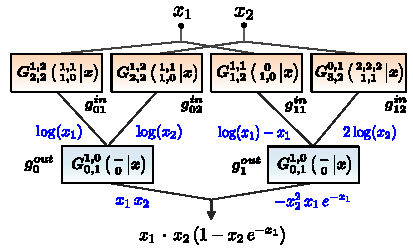
\includegraphics[width=4.5in]{ch3Fig3.pdf}
\caption{Schematic for the metamodel in Figure \ref{ch3fig1}.}
\label{ch3fig3} 
\end{figure*}

\subsection{Optimizing symbolic metamodels via gradient descent}
\label{ch3Sec33} 
Another advantage of the parameterization in (\ref{ch3eq5}) is that the gradients of the $G$ function with respect to its parameters can be approximated in analytic form as follows \cite{beals2013meijer}: 
\begin{align}
\frac{d}{da_k}\,\MeijerG{m}{n}{p}{q}{{\bf a}_p}{{\bf b}_q}{x} &\approx x^{a_k - 1} \cdot \MeijerG{m}{n+1}{p+1}{q}{-1, a_1-1,.\,.\,.,a_n-1,a_{n+1}-1,.\,.\,.,a_{p}-1}{b_1,.\,.\,.,b_m,b_{m+1},.\,.\,.,b_{q}}{x},\, 1 \leq k \leq p, \nonumber \\
\frac{d}{db_k}\,\MeijerG{m}{n}{p}{q}{{\bf a}_p}{{\bf b}_q}{x} &\approx x^{1-b_k} \cdot \MeijerG{m}{n}{p}{q+1}{a_1,.\,.\,.,a_n,a_{n+1},.\,.\,.,a_{p}}{b_1-1,.\,.\,.,b_m-1,0,b_{m+1}-1,.\,.\,.,b_{q}-1}{x}\, 1 \leq k \leq q.
\label{ch3eq6}
\end{align}
From (\ref{ch3eq6}), we see that the approximate gradient of a $G$ function is also a $G$ function, and hence the optimization problem in (\ref{ch3eq2}) can be solved efficiently via standard gradient descent algorithms.

The solution to the metamodel optimization problem in (\ref{ch3eq2}) must be confined to a predefined space of expressions $\mathcal{G}$. In particular, we consider the following classes of expressions: 
\begin{align}
\mbox{\footnotesize \bf Polynomial expressions} \boldsymbol{\subset} \mbox{\footnotesize  \bf Algebraic expressions} \boldsymbol{\subset} \mbox{\footnotesize \bf Closed-form expressions} \boldsymbol{\subset} \mbox{\footnotesize \bf Analytic expressions}, \nonumber
\end{align}
where the different classes of mathematical expressions correspond to different levels of metamodel complexity, with polynomial metamodels being the least complex (See Figure \ref{ch3fig2}).

Algorithm 1 summarizes all the steps involved in solving the metamodel optimization problem. The algorithm starts by drawing $n$ feature points uniformly at random from the feature space $[0,1]^d$ --- these feature points are used to evaluate the predictions of both the model and the metamodel in order to estimate the metamodeling loss in (\ref{ch3eq1}). Gradient descent is then executed using the gradient estimates in (\ref{ch3eq6}) until convergence. (Any variant of gradient descent can be used.) We then check if every basis function in the resulting metamodel $g({\bf x})$ lies in $\mathcal{G}$. If $g({\bf x}) \notin \mathcal{G}$, we search for an approximate version of the metamodel $\tilde{g}({\bf x}) \approx g({\bf x})$, such that $\tilde{g}({\bf x}) \in \mathcal{G}$.  

\begin{algorithm}[H]
        $ $\\[.5ex]
        $\mbox{\tiny $\blacksquare$}$ \mbox{\footnotesize {\bf Input:}} \mbox{\footnotesize Model $f({\bf x})$, hyperparameters $(m,n,p,q,r)$} \\[1ex]
        $\mbox{\tiny $\blacksquare$}$ \mbox{\footnotesize {\bf Output:}} \mbox{\footnotesize Metamodel $g({\bf x}) \in \mathcal{G}$} \vspace{0.1in} \hrule
        $ $\\[.5ex]  
        $\mbox{$\bullet$}$ \mbox{\footnotesize$X_i \sim \mbox{Unif}([0,1]^d),\, i = \{1,.\,.\,.,n\}$.} \\[1ex] %\vspace{0.05in} %
$\mbox{$\bullet$}$ \mbox{\footnotesize {\bf Repeat until convergence:}} \\[1ex]
\textcolor{white}{$ .$$ .$$ .$$ .$$ .$$ .$}\mbox{\footnotesize $\theta^{k+1} \defeq \theta^{k} - \gamma\,\nabla_{\theta}\sum_i\ell(G(X_i;\theta), f(X_i))\big|_{\theta = \theta_k}$} \\ %[1ex]
$\mbox{$\bullet$}$  \mbox{\footnotesize $g({\bf x}) \gets G(X_i;\theta^{k})$} \\ [1ex]        
$\mbox{$\bullet$}$ \mbox{\footnotesize {\bf If} $g({\bf x}) \notin \mathcal{G}$:} \\[1ex]
\textcolor{white}{$ .$$ .$$ .$$ .$$ .$$ .$}\mbox{\footnotesize $\tilde{g}({\bf x}) = G({\bf x};\bar{\theta}),\, G({\bf x};\bar{\theta}) \in \mathcal{G}, \|\bar{\theta}-\theta^k\|  < \delta$, or} \\
\textcolor{white}{$ .$$ .$$ .$$ .$$ .$$ .$}\mbox{\footnotesize $\tilde{g}({\bf x}) = \mbox{Chebyshev}(g({\bf x}))$}\vspace{0.05in} %\\ % 
        \caption{Symbolic Metamodeling}
        \end{algorithm}

\section{Related Work: Symbolic Metamodels as Gateways to Interpretation}
\label{ch3sec4}
The strand of literature most relevant to our work is the work on {\it symbolic regression} \cite{orzechowski2018we,menezes2014symbolic,vladislavleva2009order}. This is a regression model that searches a space of mathematical expressions using {\it genetic programming}. The main difference between this method and ours is that symbolic regression requires predefining the functional forms to be searched over, hence the number of its parameters increases with the number of functions that it can fit. On the contrary, our Meijer $G$-function parameterization enables recovering infinitely many functional forms through a fixed-dimensional parameter space, and allows optimizing metamodels via gradient descent. We compare our method with symbolic regression in Section \ref{ch3Sec5}. \\
\\
{\bf Symbolic metamodeling as a unifying framework for interpretation.} We now demonstrate how symbolic metamodeling can serve as a {\it gateway} to the different forms of model explanation covrered in the literature. To vivify this view, we go through common types of model explanation, and show that given $g({\bf x})$ we can recover these explanations via analytic manipulation of $g({\bf x})$. 

The most common form of model explanation involves computing importance scores of each feature dimension in ${\bf x}$ on the prediction of a given instance. Examples for methods that provide this type of explanation include SHAP \cite{lundberg2017unified}, INVASE \cite{yoon2018invase}, DeepLIFT \cite{shrikumar2017learning}, L2X \cite{chen2018learning}, LIME \cite{elenberg2017streaming,ribeiro2016should}, GAM \cite{hastie2017generalized}, and Saliency maps \cite{simonyan2013deep}. Each of these methods follows one of two approaches. The first approach, adopted by saliency maps, use the {\it gradients} of the model output with respect to the input as a measure of feature importance. The second approach, followed by LIME, DeepLIFT, GAM and SHAP, uses {\it local additive approximations} to explicitly quantify the additive contribution of each feature.

Symbolic metamodeling enables a {\it unified} framework for (instancewise) feature importance scoring that encapsulates the two main approaches in the literature. To show how this is possible, consider the following Taylor expansion of the metamodel $g({\bf x})$ around a feature point ${\bf x}_0$:   
\begin{equation}
g({\bf x}) = g({\bf x}_0) \,\, + \,\, ({\bf x} - {\bf x}_0) \cdot \nabla_{{\bf x}}\, g({\bf x}_0) \,\, + \,\, ({\bf x} - {\bf x}_0) \cdot \boldsymbol{H}({\bf x}) \cdot ({\bf x} - {\bf x}_0) \,\, + \,\,\,.\,.\,.\,.,
\label{eqTaylor}
\end{equation}
where $\boldsymbol{H}({\bf x}) = [\partial^2 g/\partial x_i \partial x_j]_{i,j}$ is the Hessian matrix. Now consider --- for simplicity of exposition --- a second-order approximation of (\ref{eqTaylor}) with a two-dimensional feature space ${\bf x} = (x_1,x_2)$, i.e.,
\begin{align}
g({\bf x}) \approx \,\, g({\bf x}_0) \,\,&+\,\,\color{blue}{(x_1-x_{0,1})\cdot g_{x_1}({\bf x}_0) - x_{0,2}\cdot x_1 \cdot g_{x_1x_2}({\bf x}_0) + \mbox{\footnotesize $\frac{1}{2}$}\,(x_1-x_{0,1})^2\,g_{x_1x_1}({\bf x}_0)}\,\,  \nonumber \\ 
&+\,\,\color{red}{(x_2-x_{0,2})\cdot g_{x_2}({\bf x}_0) - x_{0,1} \cdot x_2 \cdot g_{x_1x_2}({\bf x}_0) + \mbox{\footnotesize $\frac{1}{2}$}\,(x_2-x_{0,2})^2\,g_{x_2x_2}({\bf x}_0)} \nonumber \\ 
&+\,\,\color{blue}{x_1}\,\color{black}{\cdot}\,\color{red}{x_2}\,\color{black}{\cdot}\,\color{black}{g_{x_1x_2}({\bf x}_0),}
\label{eqTaylor2}
\end{align}
where $g_x = \nabla_x\, g$ and ${\bf x}_0 = (x_{0,1},x_{0,2})$. In (\ref{eqTaylor2}), the term in blue (first line) reflects the importance of feature $\color{blue}{x_1}$, the term in red (second line) reflects the importance of feature $\color{red}{x_2}$, whereas the last term (third line) is the interaction between the two features. The first two terms are what generalized additive~models,~such as GAM and SHAP, compute. LIME is a special case of (\ref{eqTaylor2}) that corresponds to a first-order Taylor approximation. Similar to saliency methods, the feature contributions in (\ref{eqTaylor2}) are computed using the gradients of the model with respect to the input, but (\ref{eqTaylor2}) is more general as it involves higher order gradients to capture the feature contributions more accurately. All the gradients in (\ref{eqTaylor2}) can be computed efficiently since the exact gradient of the $G$ function with respect to its input can be represented analytically in terms of another $G$ function.

Statistical interactions between features are another form of model interpretation that has been recently addressed in \cite{lou2013accurate,tsang2018neural}. As we have seen in (\ref{eqTaylor2}), feature interactions can be analytically derived from a symbolic metamodel. The series in (\ref{eqTaylor2}) resembles the structure of the pairwise interaction model \mbox{\footnotesize GA$^2$M} in \cite{lou2013accurate} and the NIT disentanglement method in \cite{tsang2018neural}. Unlike both methods, a symbolic metamodel can analytically quantify the strength of higher-order (beyond pairwise) interactions with no extra algorithmic complexity. Moreover, unlike the NIT model in \cite{tsang2018neural}, which is tailored to neural networks, a symbolic metamodel can quantify the interactions in any machine learning model (\ref{eqTaylor}). 


\begin{table}[h]
\centering 
\caption{Comparison between SM and SR.}
   \begin{tabular}{lcccc} % alignment of each column data
   \toprule[\heavyrulewidth]\toprule[\heavyrulewidth]
           & {\color{black}{\mbox{\footnotesize $\boldsymbol{f_1(x) = e^{-3x}}$}}} & {\color{black}{\mbox{\footnotesize $\boldsymbol{f_2(x) = \frac{x}{(x+1)^2}}$}}} & {\color{black}{\mbox{\footnotesize $\boldsymbol{f_3(x) = \sin(x)}$}}} & {\color{black}{\mbox{\footnotesize $\boldsymbol{f_4(x) = J_0(10\sqrt{x})}$}}}  \\ %[.75ex]
   \midrule 
   {\footnotesize {\bf SM$^p$}} & \mbox{\footnotesize $-x^3 + \frac{5}{2}(x^2-x)+1$} & \mbox{\footnotesize $\frac{x^3}{3}-\frac{4x^2}{5}+\frac{2x}{3}$} & \mbox{\footnotesize $\frac{-1}{4}\,x^2+x$} & \mbox{\footnotesize $-7\,(x^2-x)-1.4$} \\[.5ex]
    & {\footnotesize $R^2$: $0.995$} & {\footnotesize $R^2$: $0.985$} & {\footnotesize {\bf \mbox{\footnotesize $R^2: 0.999$}}} & {\footnotesize {\bf \mbox{\footnotesize $R^2: -4.75$}}} \\
\midrule
   {\footnotesize {\bf SM$^c$}} & \mbox{\footnotesize $x^{4 \times 10^{-6}}e^{-2.99x}$} & \mbox{\footnotesize $x\,(x+1)^{-2}$} & \mbox{\footnotesize $1.4\,x^{1.12}$} & \mbox{\footnotesize $I_{0.0003}\left(10\,e^{\frac{j\pi}{2}}\,\sqrt{x}\right)$} \\[1ex]
    & {\footnotesize $R^2$: $0.999$} & {\footnotesize $R^2$: $0.999$} & {\footnotesize {\bf \mbox{\footnotesize $R^2: 0.999$}}} & {\footnotesize {\bf \mbox{\footnotesize $R^2: 0.999$}}} \\    
     \midrule
   {\footnotesize {\bf SR}} & \mbox{\footnotesize $x^2 - 1.9x + 0.9$} & \mbox{\footnotesize $\frac{0.7x}{x^2 + 0.9x + 0.75}$} & \mbox{\footnotesize $-0.17\,x^2 + x + 0.016$} & \mbox{\footnotesize $-x\,(x-0.773)$} \\[.5ex]
    & {\footnotesize $R^2$: $0.970$} & {\footnotesize $R^2$ $0.981$} & {\footnotesize {\bf \mbox{\footnotesize $R^2: 0.998$}}} & {\footnotesize {\bf \mbox{\footnotesize $R^2: 0.116$}}} \\
   \bottomrule[\heavyrulewidth] 
   \end{tabular}
  \label{ch3Table2}
\end{table}

\section{Experiments}
\label{ch3Sec5}
Building on the discussions in Section \ref{ch3sec4}, we demonstrate the use cases of symbolic metamodeling through experiments on synthetic and real data. In all experiments, we used \texttt{Sympy} \cite{10.7717/peerj-cs.103} (a symbolic computation library in Python) to carry out computations involving Meijer $G$-functions.

\subsection{Learning Uni-variate Symbolic Expressions} 
\label{Sec51}

We start off with four synthetic experiments with the aim of evaluating the richness of symbolic expressions discovered by our metamodeling algorithm. In each experiment, we apply Algorithm~1 (Section \ref{ch3Sec33}) on a ground-truth univariate function $f(x)$ to fit a metamodel $g(x) \approx f(x)$, and compare the resulting mathematical expression for $g(x)$ with that obtained by Symbolic regression \cite{orzechowski2018we} implemented using \texttt{gplearn} library \cite{stephens2015gplearn}.

In Table \ref{ch3Table2}, we compare symbolic metamodeling (SM) and symbolic regression (SR) in terms of the expressions they discover and their $R^2$ coefficient with respect to the true functions. We consider four functions: an exponential $e^{-3x}$, a rational $x/(x+1^2)$, a sinusoid $\sin(x)$ and a {\it Bessel function} of the first kind $J_0(10\sqrt{x})$. We consider two versions of SM: $\mbox{SM}^{p}$ for which $\mathcal{G}=\mbox{Polynomial expressions}$, and $\mbox{SM}^{c}$ for which $\mathcal{G}=\mbox{Closed-form expressions}$. As we can see, SM is generally more accurate and more expressive than SR. For $f_1(x)$, $f_2(x)$ and $f_4(x)$, SM managed to figure out the functional forms of the true functions  ($J_0(x) = I_{0}(e^{\frac{j\pi}{2}}\,x)$, where $I_0(x)$ is the {\it Bessel function of the second kind}. For $f_3(x)$, $\mbox{SM}^{c}$ recovered a parsimonious approximation $g_3(x)$ since $\sin(x) \approx x$ for $x \in [0,1]$. Moreover, $\mbox{SM}^{p}$ managed to retrieve more accurate polynomial expressions than SR. 

\subsection{ Instance-wise feature importance} 
\label{Sec52}
Now we evaluate the ability of symbolic metamodels to explain predictions in terms of instancewise feature importance (Section \ref{ch3sec4}). To this end, we replicate the experiments in \cite{chen2018learning} with the following synthetic data sets: {\it XOR}, {\it Nonlinear additive features}, and {\it Feature switching}. (See Section 4.1 in \cite{chen2018learning} or Appendix B for a detailed description of the data sets.) Each data set has a 10-dimensional feature space and 1000 data samples.

For each of the three data sets above, we fit a 2-layer neural network $f({\bf x})$ (with 200 hidden units) to predict the labels based on the 10 features, and then fit a symbolic metamodel $g({\bf x})$ for the trained network $f({\bf x})$  using the algorithm in Section \ref{ch3Sec33}. Instancewise feature importance is derived using the (first-order) Taylor approximation in (\ref{eqTaylor2}). Since the underlying true features are known for each sample, we use the median feature importance ranking of each algorithm as a measure of the accuracy of its feature ranks as in \cite{chen2018learning}. Lower median ranks correspond to more accurate algorithms. 

\begin{figure*}[t]
\centering
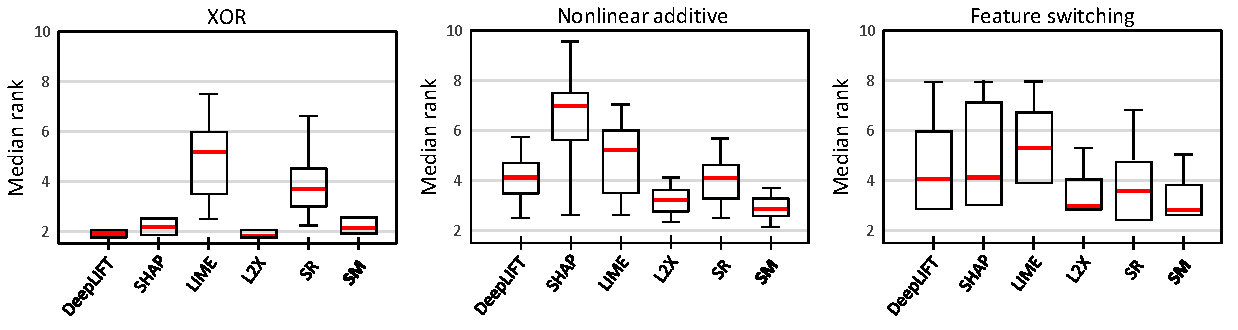
\includegraphics[width=6.5in]{ch3Fig4.pdf}
\caption{Box-plots for the median ranks of features by their estimated importance per sample over the 1000 samples of each data set. The red line is the median. Lower median ranks are better.}
\label{ch3fig4} 
\end{figure*}

In Figure \ref{ch3fig4}, we compare the performance of metamodeling (SM) with DeepLIFT, SHAP, LIME, and L2X. We also use the Taylor approximation in (\ref{eqTaylor2}) to derive feature importance scores from a symbolic regression (SR) model as an additional benchmark. For all data sets, SM performs competitively compared to L2X, which is optimized specifically to estimate instancewise feature importance. Unlike LIME and SHAP, SM captures the strengths of feature interactions, and consequently it provides more modes of explanation even in the instances where it does not outperform the additive methods in terms of feature ranking. Moreover, because SM recovers more accurate symbolic expressions than SR, it provides a more accurate feature ranking as a result.

\chapter{Automated Prognostic Modeling}
Given the abundance of ML-based predictive and causal models, which model should we use for the dataset at hand? Despite a variety of ML-based modeling options at our disposal, there is, however, a concerning gap between the potential and actual utilization of ML in prognostic research; the reason being that clinicians with no expertise in data science find it hard to manually design and tune ML pipelines \cite{luo2017automating}. To fill this gap, we developed {\footnotesize \textsc{AutoPrognosis}}, an automated ML (AutoML) framework tailored for clinical prognostic modeling that encapsulates the modules presented in the previous Chapters, and automates their design choices. {\footnotesize \textsc{AutoPrognosis}} takes as an input data from a patient cohort, and uses such data to automatically configure ML {\it pipelines}. Every ML pipeline comprises all stages of prognostic modeling: missing data imputation, feature preprocessing, prediction, and calibration. An overview of the system is provided in Figure \ref{ch4fig1}. 

\begin{figure}[h]
\centering
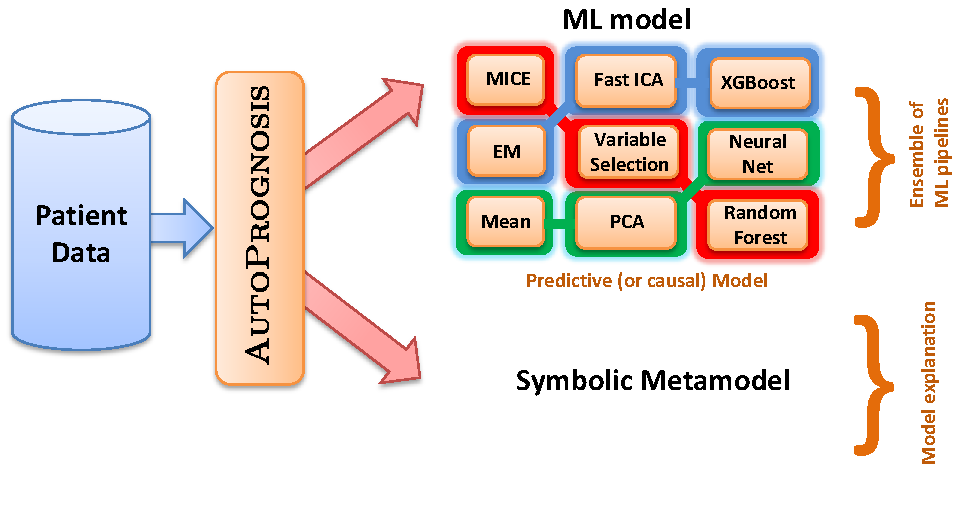
\includegraphics[width=4in]{ch4Fig1.pdf}
\caption{High-level illustration for \textsc{AutoPrognosis}.}
\label{ch4fig1} 
\end{figure}

The core component of {\footnotesize \textsc{AutoPrognosis}} is an algorithm for configuring ML pipelines using Bayesian optimization (BO) \cite{snoek2012practical}. Our BO algorithm models the pipelines' performances as a black-box function, the input to which is a ``pipeline configuration", i.e. a selection of algorithms and hyperparameter settings, and the output of which is the performance (predictive accuracy) achieved by such a configuration. We implement BO with a {\it Gaussian process} (GP) prior on the black-box function. To deal with the high-dimensionality of the pipeline configuration space, we capitalize on the fact that for a given dataset, {\bf the performance of one ML algorithm may not be correlated with that of another algorithm}. For instance, it may be the case that the observed empirical performance of {\it logistic regression} on a given dataset does not tell us much information about how a {\it neural network} would perform on the same dataset. In such a case, both algorithms should not share the same GP prior, but should rather be modeled independently. Our BO {\bf learns} such a decomposition of algorithms from data in order to break down the high-dimensional optimization problem into a set of lower-dimensional sub-problems. We model the decomposition of algorithms via an additive kernel with a Dirichlet prior on its structure, and learn the decomposition from data in concurrence with the BO iterations. We also propose a batched (parallelized) version of the BO procedure, along with a computationally efficient algorithm for maximizing the BO acquisition function. 

In addition to the causal models we proposed in Chapter 2, numerous machine learning-based models for causal inference were developed in the past few years, capitalizing on ideas from representation learning \cite{yao2018representation}, multi-task learning \cite{alaa2018limits} and adversarial training \cite{jjschaar}. The literature on machine learning-based causal inference is constantly growing, with various related workshops and competitions being held every year \cite{dorie2017automated}. Automating the selection of ML causal models is tricky since it is impossible to know what the counterfactual outcome would have been had patients received an alternative treatment. Since causal effects are determined by both factual and counterfactual outcomes, ground-truth effects can never be measured in an observational study, and hence empirical validation of causal modeling choices is anything but straightforward \cite{stuart2013estimating}.

To address this issue, we use influence functions --- a key technique in robust statistics and efficiency theory \cite{hampel2011robust,robins2008higher} --- to develop a model validation procedure that estimates the performance of causal inference methods applied to a given observational dataset {\bf without the need to access counterfactual data}, in order to enable the {\footnotesize \textsc{AutoPrognosis}} system to select among causal inference models. To the best of our knowledge, ours is the first validation procedure for models of individualized causal effects. Our procedure can be easily extended to other under-explored problems involving unlabeled data, such as semi-supervised learning \cite{oliver2018realistic}.

\section{Overview of Related Literature}
\label{ch4sec1}
\subsection{Automated ML and Bayesian Optimization}
To the best of our knowledge, none of the existing AutoML frameworks, such as {\footnotesize \textsc{Auto-Weka}} \cite{kotthoff2016auto}, {\footnotesize \textsc{Auto-sklearn}} \cite{feurer2015efficient}, and {\footnotesize \textsc{TPOT}} \cite{olson2016tpot} use principled GP-based BO to configure ML pipelines. All of the existing frameworks model the sparsity of the pipelines' hyperparameter space via frequentist tree-based structures. Both {\footnotesize \textsc{Auto-Weka}} and {\footnotesize \textsc{Auto-sklearn}} use BO, but through tree-based heuristics, such as random forest models and tree Parzen estimators, whereas TPOT uses a tree-based genetic programming algorithm. Previous works have refrained from using principled GP-based BO because of its statistical and computational complexity in high-dimensional hyperparameter spaces. Our algorithm makes principled, high-dimensional GP-based BO possible by {\bf learning} a sparse additive kernel decomposition for the GP prior. This approach confers many advantages as it captures the uncertainty about the sparsity structure of the GP prior, and allows for principled approaches for (Bayesian) meta-learning and ensemble construction that are organically connected to the BO procedure. 

Various previous works have addressed the problem of high-dimensional GP-based BO. \cite{wang2013bayesian} identifies a low-dimensional effective subspace for the black-box function via random embedding. However, in the AutoML setup, this approach cannot incorporate our prior knowledge about dependencies between the different hyperparameters (we know the sets of hyperparameters that are ``activated" upon selecting an algorithm \cite{hutter2011sequential}). This prior knowledge was captured by the {\it Arc-kernel} proposed in \cite{swersky2014raiders}, and similarly in \cite{jenatton2017bayesian}, where a BO algorithm for domains with tree-structured dependencies was proposed. Unfortunately, both methods require full prior knowledge of the dependencies between the hyperparameters, and hence cannot be used when jointly configuring hyperparameters across multiple algorithms, since the correlations of the performances of different algorithms are not known a priori. \cite{bergstra2011implementations} proposed a na\"ive approach that defines an independent GP for every set of hyperparameters that belong to the same algorithm. Since it does not share any information between the different algorithms, this approach would require trying all combinations of algorithms in a pipeline exhaustively. (In our system, there are 4,800 possible pipelines.) Our model solves the problems above via a {\bf data-driven} kernel decomposition, through which only relevant groups of hyperparameters share a common GP prior, thereby balancing the trade-off between ``information sharing" among hyperparameters and statistical efficiency. 

\subsection{Causal Model Validation}
Researchers developing new methods for causal inference validate their models using synthetic data-generating distributions that encode pre-specified causal effects --- e.g., \cite{hill2011bayesian,wager2017estimation,powers2017some}. However, such synthetic distributions bear very little resemblance to real-world data, and hence are not informative of what methods would actually work best on a given real-world observational study \cite{setoguchi2008evaluating}. Because no single model will be superior on all observational studies \cite{dorie2017automated}, model selection must be guided by a data-driven validation procedure.

While the literature is rich with causal inference models, it falls short of rigorous methods for validating those models on real-world data. Applied researchers currently rely on simple heuristics to predict a model's performance on a given dataset \cite{schuler2017synth,rolling2014model,van2003unified}, but such heuristics do not provide any theoretical guarantees, and can fail badly in certain scenarios \cite{schuler2018general}.

Despite their popularity in statistics, influence functions are seldom used in machine learning. Recently in \cite{koh2017understanding}, influence functions were used for interpreting black-box models by tracing the impact of data points on a model's predictions. Our usage of influence functions differs from \cite{koh2017understanding} in that we use them to construct efficient estimators of a model's loss and not to explain the inner workings of a learning algorithm. In that sense, our work is more connected to the literature on plug-in estimation and nonparametric efficiency theory \cite{goldstein1992optimal,robins2008higher,robins2017minimax,van2014higher}.     

\section{\textsc{AutoPrognosis}: A System for Automated Prognostic Modeling}
\label{ch4sec2}
We start with the predictive modeling setup, where our goal is to automate the design of predictive models for the dataset at hand. Consider a dataset $\mathcal{D} = \{(x_i,y_i)\}^n_{i=1}$ for a cohort of $n$ patients, with $x_i$ being patient $i$'s features, and $y_i$ being the patient's clinical endpoint. {\footnotesize \textsc{AutoPrognosis}} takes $\mathcal{D}$ as an input, and outputs an automatically configured {\it prognostic model} which predicts the patients' risks. This Section provides an overview of the components of {\footnotesize \textsc{AutoPrognosis}}.  

The core component of {\footnotesize \textsc{AutoPrognosis}} is an algorithm that automatically configures ML pipelines, where every pipeline comprises algorithms for missing data imputation (${\tiny \square}$), feature preprocessing (${\tiny \clubsuit}$), prediction ($\bullet$), and calibration (${\tiny \bigstar}$). Table \ref{ch4Table1} lists the baseline algorithms adopted by the system in all the stages of a pipeline. The imputation and calibration stages are particularly important for clinical prognostic modeling \cite{blaha2016critical}, and are not supported in existing AutoML frameworks. The total number of hyperparameters in {\footnotesize \textsc{AutoPrognosis}} is 106, which is less than those of {\footnotesize \textsc{Auto-Weka}} (786) and {\footnotesize \textsc{Auto-sklearn}} (110). The pipeline configuration algorithm uses {\bf Bayesian optimization} to estimate the performance of different pipeline configurations in a {\bf scalable} fashion by learning a {\bf structured kernel decomposition} that identifies algorithms with {\it correlated} performance. Details of the Bayesian optimization algorithm are provided in Sections \ref{ch4sec3}.

\begin{table*}[t]%[!htbp]
\centering
%\begin{tcolorbox}[tab3,tabularx={l||lllll}]
\begin{tabular}{|l||llll|}
\hline
{\bf {\footnotesize Pipeline Stage}} & & {\footnotesize {\bf Algorithms}}& &   \\
\hline
\hline
{\tiny \bf $\square$} {\footnotesize Data Imputation} & {\tiny $\square$} {\footnotesize missForest {\bf \textcolor{brown}{(2)}}} & {\tiny $\square$} {\footnotesize Median {\bf \textcolor{brown}{(0)}}} & {\tiny $\square$} {\footnotesize Most-frequent {\bf \textcolor{brown}{(0)}}} & {\tiny $\square$} {\footnotesize Mean {\bf \textcolor{brown}{(0)}}}   \\
& {\tiny $\square$} {\footnotesize Matrix completion {\bf \textcolor{brown}{(2)}}} & {\tiny $\square$} {\footnotesize MICE {\bf \textcolor{brown}{(1)}}} & {\tiny $\square$} {\footnotesize None {\bf \textcolor{brown}{(0)}}} & {\tiny $\square$} {\footnotesize EM {\bf \textcolor{brown}{(1)}}}  \\
\hline \hline
{\tiny $\clubsuit$} {\footnotesize Feature process.} & {\tiny $\clubsuit$} {\footnotesize Feature agglo. {\bf \textcolor{brown}{(4)}}} & {\tiny $\clubsuit$} {\footnotesize Kernel PCA {\bf \textcolor{brown}{(5)}}} & {\tiny $\clubsuit$} {\footnotesize Polynomial {\bf \textcolor{brown}{(3)}}} & {\tiny $\clubsuit$} {\footnotesize Fast ICA {\bf \textcolor{brown}{(4)}}}   \\
& {\tiny $\clubsuit$} {\footnotesize R. kitchen sinks {\bf \textcolor{brown}{(2)}}} & {\tiny $\clubsuit$} {\footnotesize Nystroem {\bf \textcolor{brown}{(5)}}} & {\tiny $\clubsuit$} {\footnotesize Linear SVM {\bf \textcolor{brown}{(3)}}} & {\tiny $\clubsuit$} {\footnotesize Select Rates {\bf \textcolor{brown}{(3)}}}  \\
& {\tiny $\clubsuit$} {\footnotesize PCA {\bf \textcolor{brown}{(2)}}} & {\tiny $\clubsuit$} {\footnotesize None {\bf \textcolor{brown}{(0)}}} & &  \\ 
\hline \hline
{\footnotesize $\bullet$ Prediction} & {\footnotesize $\bullet$ Bernoulli NB {\bf \textcolor{brown}{(2)}}} & {\footnotesize $\bullet$ AdaBoost {\bf \textcolor{brown}{(4)}}} & {\footnotesize $\bullet$ Decision Tree {\bf \textcolor{brown}{(4)}}} & {\footnotesize $\bullet$ Grad. Boost. {\bf \textcolor{brown}{(6)}}}  \\
 & {\footnotesize $\bullet$ Gaussian NB {\bf \textcolor{brown}{(0)}}} & {\footnotesize $\bullet$ XGBoost {\bf \textcolor{brown}{(5)}}} & {\footnotesize $\bullet$ Extr. R. Trees {\bf \textcolor{brown}{(5)}}} & {\footnotesize $\bullet$ Light GBM {\bf \textcolor{brown}{(5)}}}  \\
 & {\footnotesize $\bullet$ Multinomial NB {\bf \textcolor{brown}{(2)}}} & {\footnotesize $\bullet$ R. Forest {\bf \textcolor{brown}{(5)}}} & {\footnotesize $\bullet$ Neural Net. {\bf \textcolor{brown}{(5)}}} & {\footnotesize $\bullet$ Log. Reg. {\bf \textcolor{brown}{(0)}}}  \\
 & {\footnotesize $\bullet$ Ridge Class. {\bf \textcolor{brown}{(1)}}} & {\footnotesize $\bullet$ Bagging {\bf \textcolor{brown}{(4)}}} & {\footnotesize $\bullet$ $k$-NN {\bf \textcolor{brown}{(1)}}} & {\footnotesize $\bullet$ Surv. Forest {\bf \textcolor{brown}{(5)}}}   \\
& {\footnotesize $\bullet$ LDA {\bf \textcolor{brown}{(4)}}} & {\footnotesize $\bullet$ L. SVM {\bf \textcolor{brown}{(4)}}} & {\footnotesize $\bullet$ GP {\bf \textcolor{brown}{(3)}}} & {\footnotesize $\bullet$ Cox Reg. {\bf \textcolor{brown}{(0)}}}   \\ 
\hline \hline
{\tiny $\bigstar$} {\footnotesize Calibration} & {\tiny $\bigstar$} {\footnotesize Sigmoid {\bf \textcolor{brown}{(0)}}} & {\tiny $\bigstar$} {\footnotesize Isotonic} {\bf \textcolor{brown}{(0)}} & {\tiny $\bigstar$} {\footnotesize None {\bf \textcolor{brown}{(0)}}} & \\
\hline
%\end{tcolorbox}
\end{tabular}
\caption{List of algorithms included in every stage of the pipeline. Numbers in brackets correspond to the number of hyperparameters.}
\label{ch4Table1}
\end{table*}

\section{Pipeline Configuration via Structured Bayesian Optimization}
\label{ch4sec3}
Let $(\mathcal{A}_d,\mathcal{A}_f,\mathcal{A}_p,\mathcal{A}_c)$ be the sets of all missing data imputation, feature processing, prediction, and calibration algorithms in {\footnotesize \textsc{AutoPrognosis}} (Table \ref{ch4Table1}), respectively. A {\bf pipeline} $P$ is a tuple: 
\begin{align}
P = (A_d,A_f,A_p,A_c) \nonumber
\end{align}
where $A_v \in \mathcal{A}_v,\, \forall v \in \mbox{\footnotesize $\{d,f,p,c\}$}$. The space of all pipelines is given by $\mbox{\footnotesize $\mathcal{P} = \mathcal{A}_d \times \mathcal{A}_f \times \mathcal{A}_p \times \mathcal{A}_c$}$. Thus, a pipeline is a selection of algorithms from the elements of Table \ref{ch4Table1}. An exemplary pipeline can be specified as follows: $\mbox{\footnotesize \bf $P = \{\mbox{\footnotesize \bf MICE}, \mbox{\footnotesize \bf PCA}, \mbox{\footnotesize \bf Random Forest},\mbox{\footnotesize \bf Sigmoid}\}$}$. The total number of pipelines in {\footnotesize \textsc{AutoPrognosis}} is $|\mathcal{P}| = 4,800$.

The specification of a {\bf pipeline configuration} is completed by determining the hyperparameters of its constituting algorithms. The space of hyperparameter configurations for a pipeline is $\Theta = \Theta_d \times \Theta_f \times \Theta_p \times \Theta_c$, where $\Theta_v = \cup_{a}\Theta^{a}_v$, for $v \in \mbox{\footnotesize $\{d,f,p,c\}$},$ with $\Theta^{a}_v$ being the space of hyperparameters associated with the $a^{th}$ algorithm in $\mathcal{A}_v$. Thus, a pipeline configuration $P_\theta \in \mathcal{P}_{\Theta}$ is a selection of algorithms $P \in \mathcal{P}$, and hyperparameter settings $\theta \in \Theta$; $\mathcal{P}_{\Theta}$ is the space of all possible pipeline configurations.

\subsection{The Pipeline Selection \& Configuration Problem}

The main goal of {\footnotesize \textsc{AutoPrognosis}} is to identify the best pipeline configuration $P^*_{\theta^*} \in \mathcal{P}_{\Theta}$ for a given patient cohort $\mathcal{D}$ via $J$-fold cross-validation as follows: 
\begin{align}
P^*_{\theta^*} \in \arg \max_{P_\theta \in \mathcal{P}_\Theta}\, \frac{1}{J}\sum_{i=1}^{J}\mathcal{L}(P_\theta;\mathcal{D}^{(i)}_{\mbox{\tiny train}},\mathcal{D}^{(i)}_{\tiny \mbox{valid}}),
\label{ch4eq1}
\end{align}
where $\mathcal{L}$ is a given accuracy metric (AUC-ROC, c-index, etc), $\mathcal{D}^{(i)}_{\mbox{\tiny train}}$ and $\mathcal{D}^{(i)}_{\tiny \mbox{valid}}$ are training and validation splits of $\mathcal{D}$ in the $i^{th}$ fold. The optimization problem in (\ref{ch4eq1}) is dubbed the {\it Pipeline Selection and Configuration Problem} (PSCP). The PSCP can be thought of as a generalization for the {\it combined algorithm selection and hyperparameter optimization} (CASH) problem in \cite{feurer2015efficient,kotthoff2016auto}, which maximizes an objective with respect to selections of single algorithms from the set $\mathcal{A}_p$, rather than selections of full-fledged pipelines from $\mathcal{P}_{\Theta}$.

\subsection{Solving the PSCP via Bayesian Optimization}

The objective in (\ref{ch4eq1}) has no analytic form, and hence we treat the PSCP as a {\it black-box} optimization problem. In particular, we assume that $\mbox{\footnotesize $\frac{1}{J}\sum_{i=1}^{J}\mathcal{L}(P_\theta;\mathcal{D}^{(i)}_{\mbox{\tiny train}},\mathcal{D}^{(i)}_{\tiny \mbox{valid}})$}$ is a noisy version of a black-box function $\mbox{\footnotesize $f: {\bf \Lambda} \to \mathbb{R}$}$, were $\mbox{\footnotesize ${\bf \Lambda} = \Theta \times \mathcal{P}$}$, and use BO to search for the pipeline configuration $P^*_{\theta^*}$ that maximizes the black-box function $f(.)$ \cite{snoek2012practical}. The BO algorithm specifies a Gaussian process (GP) prior on $f(.)$ as follows:
\begin{align}
f \sim \mathcal{GP}(\mu(\Lambda),k(\Lambda,\Lambda^{\prime})),
\label{eq10X}
\end{align}
where $\mu(\Lambda)$ is the {\it mean function}, encoding the expected performance of different pipeline, and $k(\Lambda,\Lambda^{\prime})$ is the {\it covariance kernel} \cite{rasmussen2006gaussian}, encoding the similarity between the different pipelines.

\begin{figure*}[t]
\centering
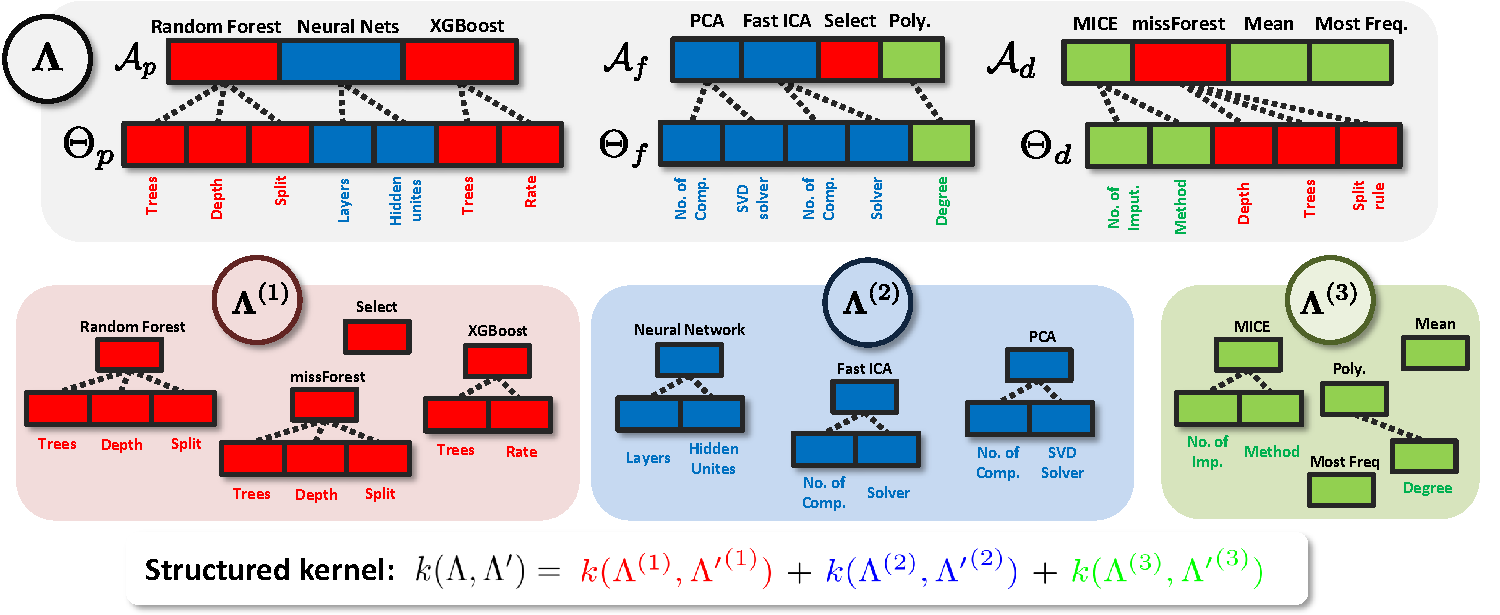
\includegraphics[width=6in]{ch4Fig2.pdf}
\caption{Illustration for a exemplary subspace decomposition $\{{\bf \Lambda}^{(m)}\}^3_{m=1}$.}
\label{ch4fig2}
\end{figure*}

\subsection{Bayesian Optimization via Structured Kernels}  
The function $f$ is defined over the \mbox{\footnotesize $D$}-dimensional space $\mbox{\footnotesize ${\bf \Lambda}$}$, where $\mbox{\footnotesize $D = \mbox{dim}({\bf \Lambda})$}$ is given by 
\begin{align}
D = \mbox{\footnotesize dim}(\mathcal{P}) + {\textstyle \sum}_{v \in \{d,f,p,c\}} {\textstyle \sum}_{a \in \mathcal{A}_v} \mbox{\footnotesize dim}(\Theta^a_v).
\label{ch4eq3}
\end{align} 
In {\footnotesize \textsc{AutoPrognosis}}, the domain $\mbox{\footnotesize ${\bf \Lambda}$}$ is high-dimensional, with $\mbox{\footnotesize $D = 106$}$. (The dimensionality of $\mbox{\footnotesize ${\bf \Lambda}$}$ can be calculated by summing up the number of pipeline stages and the number of hyperparameters in Table \ref{ch4Table1}.) High-dimensionality renders standard GP-based BO infeasible as both the sample complexity of nonparametric estimation and the computational complexity of maximizing the acquisition function are exponential in $\mbox{\footnotesize $D$}$ \cite{gyorfi2006distribution,kandasamy2015high}. For this reason, existing AutoML frameworks have refrained from using GP priors, and relied instead on scalable tree-based heuristics \cite{feurer2015efficient,kotthoff2016auto}. Despite its superior performance, recent empirical findings have shown that plain-vanilla GP-based BO is feasible only for problems with $\mbox{\footnotesize $D \leq 10$}$ \cite{wang2013bayesian}. Thus, the deployment of GP-based BO has been limited to hyperparameter optimization for single, pre-defined ML models via tools such as \texttt{Google}'s \texttt{Visier} and \texttt{HyperTune} \cite{golovin2017google}. {\footnotesize \textsc{AutoPrognosis}} overcomes this challenge by leveraging the structure of the PSCP problem as we show in what follows. 

\subsubsection{The Structure of the PSCP Problem} 
The key idea of our BO algorithm is that for a given dataset, {\bf the performance of a given group of algorithms may not be \textit{informative} of the performance of another group of algorithms}. Since the kernel \mbox{\footnotesize $k(\Lambda,\Lambda^{\prime})$} encodes the correlations between the performances of the different pipeline configurations, the underlying ``informativeness" structure that relates the different hyperparameters can be expressed via the following {\bf sparse additive kernel decomposition}:  
\begin{align}
k(\Lambda,\Lambda^{\prime}) = {\textstyle \sum}_{m=1}^{M} k_m(\Lambda^{(m)},{\Lambda^{\prime}}^{(m)}),
\label{ch4eq4}
\end{align}
where \mbox{\footnotesize $\Lambda^{(m)} \in {\bf \Lambda}^{(m)},\forall m \in \{1,.\,.\,.,M\},$} with \mbox{\footnotesize $\{{\bf \Lambda}^{(m)}\}_m$} being a set of {\it disjoint} subspaces of \mbox{\footnotesize ${\bf \Lambda}$}. (That is, \mbox{\footnotesize $\cup_m \Lambda^{(m)} = {\bf \Lambda}$}, and \mbox{\footnotesize $\Lambda^{(m)} \cap \Lambda^{(m^{\prime})} = \emptyset$}.) The subspaces are assigned mutually exclusive subsets of the dimensions of \mbox{\footnotesize ${\bf \Lambda}$}, so that \mbox{\footnotesize ${\textstyle \sum}_{m} \mbox{\footnotesize dim}(\Lambda^{(m)}) = D$}. The structure of the kernel in (\ref{ch4eq4}) is {\bf unknown} a priori, and needs to be {\bf learned from data}. The kernel decomposition breaks down $f$ as follows:
\begin{align}
f(\Lambda) = {\textstyle \sum}_{m=1}^{M} f_m(\Lambda^{(m)}).
\label{ch4eq5}
\end{align}
The additively sparse structure in (\ref{ch4eq4}) gives rise to a statistically efficient BO procedure. That is, if $f$ is $\gamma$-smooth, then our additive kernels reduce {\bf sample complexity} from \mbox{\footnotesize $\boldsymbol{O(n^{\frac{-\gamma}{2\gamma + D}})}$} to \mbox{\footnotesize $\boldsymbol{O(n^{\frac{-\gamma}{2\gamma + D_m}})}$}, where $D_m$ is the maximum number of dimensions in any subspace \cite{raskutti2009lower,yang2015minimax}. (Similar improvements hold for the cumulative regret \cite{kandasamy2015high}.)

Each subspace $\mbox{\footnotesize ${\bf \Lambda}^{(m)} \subset {\bf \Lambda}$}$ contains the hyperparameters of algorithms with correlated performances, whereas algorithms residing in two different subspaces $\mbox{\footnotesize ${\bf \Lambda}^{(m)}$}$ and $\mbox{\footnotesize ${\bf \Lambda}^{(m^{\prime})}$}$ have uncorrelated performances. Since a hyperparameter in \mbox{\footnotesize $\Theta$} is only {\it relevant} to $f(.)$ when the corresponding algorithm in \mbox{\footnotesize $\mathcal{P}$} is selected \cite{hutter2009paramils}, then the decomposition \mbox{\footnotesize $\{{\bf \Lambda}^{(m)}\}_m$} must ensure that all the hyperparameters of the same algorithm are bundled together in the same subspace. This a priori knowledge about the ``conditional relevance" of the dimensions of $\mbox{\footnotesize ${\bf \Lambda}$}$ makes it easier to learn the kernel decomposition from data. Figure \ref{ch4fig2} provides an illustration for an exemplary subspace decomposition for the hyperparameters of a set of prediction, feature processing and imputation algorithms. Since the structured kernel in (\ref{ch4eq4}) is not fully specified a priori, we propose an algorithm to learn it from the data in the next Section.  


\subsubsection{Structured Kernel Learning} % data-driven depends on data, but prior knwolded so Bayesian
{\footnotesize \textsc{AutoPrognosis}} uses a Bayesian approach to learn the subspace decomposition \mbox{\footnotesize $\{{\bf \Lambda}^{(m)}\}_m$} in concurrence with the BO procedure, where the following Dirichlet-Multinomial prior is placed on the structured kernel \cite{wang2017batched}: 
\begin{align}
\mbox{$\alpha \sim \mbox{Dirichlet}(M,\gamma),\,\, z_{v,a} \sim \mbox{Multi}(\alpha),$} 
\label{ch4eq6}
\end{align}
\mbox{\footnotesize $\forall a \in \mathcal{A}_v, {\tiny v \in \{d,f,p,c\}}$}, where \mbox{\footnotesize $\gamma = \{\gamma_m\}_m$} is the parameter of a Dirichlet prior, \mbox{\footnotesize $\alpha = \{\alpha_m\}_m$} are the Multinomial mixing proportions, and \mbox{\footnotesize $z_{v,a}$} is an indicator variable that determines the subspace to which the $a^{th}$ algorithm in \mbox{\footnotesize $\mathcal{A}_v$} belongs. The kernel decomposition in (\ref{ch4eq4}) is learned by updating the posterior distribution of \mbox{\footnotesize $\{{\bf \Lambda}^{(m)}\}_m$} in every iteration of the BO procedure. The posterior distribution over the variables \mbox{\footnotesize $\{z_{v,a}\}_{v,a}$} and \mbox{\footnotesize $\alpha$} is given by: 
\begin{align}
\mathbb{P}(z, \alpha\,|\,\mathcal{H}_t,\gamma) \propto \mathbb{P}(\mathcal{H}_t\,|\,z) \, \mathbb{P}(z\,|\alpha) \, \mathbb{P}(\alpha,\gamma),
\label{ch4eq7}
\end{align}
where \mbox{\footnotesize $z = \{z_{v,a}: \forall a \in \mathcal{A}_v, \forall v \in \{d,f,p,c\}\}$}, and \mbox{\footnotesize $\mathcal{H}_t$} is the history of evaluations of the black-box function up to iteration $t$. Since the variables \mbox{\footnotesize $\{z_{v,a}\}_{v,a}$} are sufficient statistics for the subspace decomposition, the posterior over \mbox{\footnotesize $\{{\bf \Lambda}^{(m)}\}_m$} is fully specified by (\ref{ch4eq6}) marginalized over \mbox{\footnotesize $\alpha$}, which can be evaluated using Gibbs sampling as follows:
\begin{align}
\mathbb{P}(z_{v,a} = m\,|\,z/\{z_{v,a}\},\mathcal{H}_t) \propto \mathbb{P}(\mathcal{H}_t\,|\,z) \, (|\mathcal{A}_v^{(m)}|+\gamma_{m}), \nonumber 
\end{align}
where \mbox{\footnotesize $\mathbb{P}(\mathcal{H}_t\,|\,z)$} is the GP likelihood under the kernel induced by \mbox{\footnotesize $z$}. The Gibbs sampler is implemented via the Gumble-Max trick \cite{maddison2014sampling} as follows:
\begin{align}
\omega_m & \overset{\mbox{\tiny i.i.d}}{\sim} \mbox{Gumbel}(0,1),\, m \in \{1,.\,.\,.,M\}, \label{ch4eq8}\\ 
z_{v,a} &\sim \, \arg \max_m \mathbb{P}(\mathcal{H}_t\,|\,z,z_{v,a} = m)(|\mathcal{A}_v^{(m)}|+\gamma_{m}) + \omega_m. \nonumber 
\end{align} 

\subsubsection{Exploration via Diverse Batch Selection} %PSCP
\label{BatchSec}
The BO procedure solves the PSCP problem by exploring the performances of a sequence of pipelines \mbox{\footnotesize $\{P^1_{\theta^1},P^2_{\theta^2},.\,.\,.\}$} until it (hopefully) converges to the optimal pipeline \mbox{\footnotesize $P^*_{\theta^*}$}. In every iteration \mbox{\footnotesize $t$}, BO picks a pipeline to evaluate using an {\it acquisition function} \mbox{\footnotesize $A(P_\theta; \mathcal{H}_{t})$} that balances between {\it exploration} and {\it exploitation}. \textsc{AutoPrognosis} deploys a 2-step batched (parallelized) exploration scheme that picks \mbox{\footnotesize $B$} pipelines for evaluation at every iteration \mbox{\footnotesize $t$} as follows: 

\begin{itemize}
\item {\bf \underline{Step 1:}} Select the frequentist kernel decomposition \mbox{\footnotesize $\{{\bf \hat{\Lambda}}^{(m)}\}_m$} that maximizes \mbox{\footnotesize $\mathbb{P}(z\,|\,\mathcal{H}_t)$}.
\item {\bf \underline{Step 2:}} Select the $B$ pipelines $\{P^{b}_\theta\}^B_{b=1}$ with the highest values for the acquisition function $\{A(P^b_\theta; \mathcal{H}_{t})\}^B_{b=1}$, such that each pipeline $P^{b}_\theta,\, b \in \{1,.\,.\,.,B\},$ involves a {\bf distinct prediction} algorithm from a {\bf distinct subspace} in \mbox{\footnotesize $\{{\bf \hat{\Lambda}}^{(m)}\}_m$}.
\end{itemize}
  
We use the well-known {\it Upper Confidence Bound} (UCB) as acquisition function \cite{snoek2012practical}. The decomposition in (\ref{ch4eq4}) offers an {\bf exponential speed up} in the overall {\bf computational complexity} of Step 2 since the UCB acquisition function is maximized separately for every (low-dimensional) component $f_m$; this reduces the number of computations from to \mbox{\footnotesize $\boldsymbol{\mathcal{O}(n^{-D})}$} to \mbox{\footnotesize $\boldsymbol{\mathcal{O}(n^{-D_m})}$}. The batched implementation is advantageous since sequential evaluations of \mbox{\footnotesize $f(.)$} are time consuming as it involves training the selected ML algorithms. 

Step 2 in the algorithm above encourages exploration as follows. In every iteration $t$, we select a ``diverse" batch of pipelines for which every pipeline is representative of a {\bf distinct} subspace in \mbox{\footnotesize $\{{\bf \hat{\Lambda}}^{(m)}\}_m$}. The batch selection scheme above encourages diverse exploration without the need for sampling pipelines via a determinantal point process with an exponential complexity as in \cite{kathuria2016batched,nikolov2015randomized,wang2017batched}. We also devise an efficient {\bf backward induction} algorithm that exploits the structure of a pipeline to maximize the acquisition function efficiently. 

\section{Validating Causal Models}
In the previous sections, we developed a BO procedure for conducting predictive model selection. However, for causal models, the empirical performance measure $\mathcal{L}$ cannot be straightforwardly evaluated. In this Section, we develop an efficient estimator for the empirical performance of a causal inference model based on observational data.

\subsection{Notation and Definitions}
\label{ch4sec44}
\subsubsection{Causal Inference from Observational Data}
\label{ch4sec441}
Recall from Chapter 2 the standard {\it potential outcomes} framework for modeling causal effects in observational and experimental studies \cite{rubin1974estimating,rubin2005causal}. In this framework, a ``subject" is associated with a feature $\mbox{\footnotesize $X \in \mathcal{X}$}$, a treatment assignment indicator $\mbox{\footnotesize $W \in \{0,1\}$}$, and an outcome $\mbox{\footnotesize $Y \in \mathbb{R}$}$. The outcome variable $\mbox{\footnotesize $Y$}$ takes on the value of either of the two ``potential outcomes" $\mbox{\footnotesize $Y^{\mbox{\tiny $(0)$}}$}$ and $\mbox{\footnotesize $Y^{\mbox{\tiny $(1)$}}$}$, where $\mbox{\footnotesize $Y=Y^{\mbox{\tiny $(1)$}}$}$ if the subject received the treatment ($\mbox{\footnotesize $W=1$}$), and $\mbox{\footnotesize $Y=Y^{\mbox{\tiny $(0)$}}$}$ otherwise, i.e., $\mbox{\footnotesize $Y = W\,Y^{\mbox{\tiny $(1)$}} + (1-W)\,Y^{\mbox{\tiny $(0)$}}$}$. The causal effect of the treatment on the subject is thus given by $\mbox{\footnotesize $Y^{\mbox{\tiny $(1)$}}-Y^{\mbox{\tiny $(0)$}}$}$. \\
\\ 
{\bf \mbox{\tiny $\blacksquare$}~Observational~data.}\,~In a typical observational study, we are given $\mbox{\footnotesize $n$}$ samples of the tuple $\mbox{\footnotesize $Z = (X, W, Y)$}$ drawn from a probability distribution with a parameter $\mbox{\footnotesize $\theta$}$, i.e., 
\begin{equation}
Z_1,\,.\,.\,.\,,Z_n \sim \mathbb{P}_{\theta}\,, 
\label{ch4eq9}
\end{equation}
where~$\mbox{\footnotesize $\mathbb{P}_{\theta}$}$ belongs to the family~$\mbox{\footnotesize $\mathcal{P} = \{\mathbb{P}_{\theta^{\prime}}: \theta^{\prime} \in \Theta\}$}$,~and $\mbox{\footnotesize $\Theta$}$ is the parameter space. We break down the parameter $\mbox{\footnotesize $\theta$}$ into a collection of {\it nuisance} parameters $\mbox{\footnotesize $\theta = \{\mu_0,\mu_1,\pi,\eta\}$}$, where $\mbox{\footnotesize $\mu_0$}$ and $\mbox{\footnotesize $\mu_1$}$ are the conditional potential outcomes, i.e., 
\begin{align}
\mu_{w}(x) = \mathbb{E}_{\theta}\big[\, Y^{\mbox{\tiny $(w)$}}\,|\,X = x\,\big],\, w \in \{0,1\},
\label{ch4eq10}
\end{align} 
and $\mbox{\footnotesize $\pi$}$ is the treatment assignment mechanism, i.e.
\begin{align}
\pi(x) = \mathbb{P}_{\theta}(W = 1\,|\,X = x\,), 
\label{ch4eq11}
\end{align}
whereas~$\mbox{\footnotesize $\eta(x) = \mathbb{P}_{\theta}(X=x)$}$. To ensure the generality of our analysis, we assume that $\mbox{\footnotesize $\mathcal{P}$}$ is a {\it nonparametric} family of distributions. That is, $\mbox{\footnotesize $\Theta$}$ is an infinite-dimensional parameter space, with the nuisance parameters $\mbox{\footnotesize $\{\mu_0,\mu_1,\pi,\eta\}$}$ being specified only through mild smoothness conditions.\\
\\
{\bf \mbox{\tiny $\blacksquare$}~The~causal~inference~task.}\,~The goal of causal inference is to use the samples $\mbox{\footnotesize $\{Z_i\}^n_{i=1}$}$ in order to infer the causal effect of the treatment on individual subjects based on their features, i.e., the estimand is a function $\mbox{\footnotesize $T:\mathcal{X} \rightarrow \mathbb{R}$}$, where 
\begin{align}
T(x) = \mathbb{E}_{\theta}\big[\, Y^{\mbox{\tiny $(1)$}}-Y^{\mbox{\tiny $(0)$}}\,|\,X = x\,\big].
\label{ch4eq12}
\end{align}
The function $\mbox{\footnotesize $T(x)$}$ in (\ref{ch4eq12}) is commonly known as the conditional average treatment effect (CATE)\footnote{To ensure the identification of the CATE, we assume that $\mbox{\footnotesize $\mathbb{P}_{\theta}$}$ satisfies the standard ``unconfoundedness" and ``overlap" conditions in \cite{pearl2009causality,rubin2005causal}.}. Its importance resides in the fact that it can guide {\it individualized} decision-making policies (e.g., patient-specific treatment plans or personalized advertising policies \cite{bottou2013counterfactual}). For this reason, the CATE function is the estimand of interest for almost all modern machine learning-based causal inference methods (e.g., \cite{alaa2018limits,wager2017estimation,jjschaar,yao2018representation}).\\ 
\\
{\bf \mbox{\tiny $\blacksquare$}~Accuracy~of~causal~inference.}\,~A causal inference model $\mbox{\footnotesize $\mathcal{M}$}$ maps a dataset $\mbox{\footnotesize $\{Z_i\}^n_{i=1}$}$ to an estimate $\mbox{\footnotesize $\widehat{T}(.)$}$ of the CATE. The accuracy of a model is typically characterized by the squared-$\mbox{\footnotesize $L^2$}$ loss incurred by its estimate, i.e., 
\begin{align}
\boldsymbol{\ell}_{\theta}(\widehat{T}) &\triangleq \big\|\,\widehat{T}(X) - T(X)\,\big\|^2_{\theta},
\label{ch4eq13}
\end{align}  
where $\mbox{\footnotesize $\|f(X)\|^2_{\theta} = \mathbb{E}_{\theta}[f^2(X)]$}$. The performance evaluation metric in (\ref{ch4eq13}) was dubbed the {\it precision of estimating heterogeneous effects} (PEHE) in \cite{hill2011bayesian} --- it quantifies the ability of a model to capture the heterogeneity of the causal effects of a treatment among individuals in a population. 

\subsubsection{Model Validation \& Selection}
\label{ch4sec442} 
We now consider a set of candidate causal inference models $\mbox{\footnotesize $\overrightarrow{\mathcal{M}} = \{\mathcal{M}_1,\,.\,.\,.\,,\mathcal{M}_M\}$}$. These may include, for example, different machine learning methods (e.g., Causal Gaussian processes, GAN-ITE, causal forests, etc.), different hyperparameter settings of one method, etc. Our goal is to select the best model $\mbox{\footnotesize $\mathcal{M}^{*} \in \overrightarrow{\mathcal{M}}$}$ that incurs the minimum PEHE for a given dataset.\\ 
\\
{\bf \mbox{\tiny $\blacksquare$}~Beyond~cross-validation.}\,~Evidently,~reliable~model~selection requires~a~model~validation~procedure~that~estimates the PEHE accuracy of each model in $\mbox{\footnotesize $\overrightarrow{\mathcal{M}}$}$. Unlike standard supervised learning in which all data points are definitely ``labeled", in the causal inference setting we do not have access to the ground-truth causal effect \mbox{\footnotesize $Y^{\mbox{\tiny $(1)$}}-Y^{\mbox{\tiny $(0)$}}$}. This is because in an observational dataset, we can only observe the factual outcome \mbox{\footnotesize $Y^{\mbox{\tiny $(W)$}}$}, but not the counterfactual \mbox{\footnotesize $Y^{\mbox{\tiny $(1-W)$}}$}. This renders the empirical measure of PEHE, i.e., $\mbox{\footnotesize $\frac{1}{n}\,\sum^n_{i=1}(\widehat{T}(X_i)-(Y_i^{\mbox{\tiny $(1)$}}-Y_i^{\mbox{\tiny $(0)$}}))^2$}$, incalculable from the samples \mbox{\footnotesize $\{Z_i = (X_i, W_i, Y_i)\}^n_{i=1}$}, and hence standard cross-validation techniques cannot be used to evaluate the performance of a given causal inference model\footnote{In~Appendix~B,~we~analyze a number of na\"ive alternatives to cross-validation that were used in previous works to tune the hyperparameter of causal inference models \cite{shalit2016estimating,shimodaira2000improving}, etc.). We show that all such alternatives provide either inconsistent or inefficient estimates of the PEHE.}.

\section{Causal Model Validation via Influence Functions}  
\label{ch4sec43} 
\textit{How~can~we~test~the~PEHE~performance~of~a~causal~inference model without observing a test label \mbox{\footnotesize $Y^{\mbox{\tiny $(1)$}}-Y^{\mbox{\tiny $(0)$}}$}?} To answer this question, we develop a consistent and efficient validation procedure that estimates the PEHE of any causal inference model via a statistic that {\bf does not depend on the counterfactual data} \mbox{\footnotesize $\boldsymbol{Y^{\mbox{\tiny $(1-W)$}}}$}. Using this procedure, practitioners can evaluate, compare and select causal inference models as envisioned in Section \ref{ch4sec44}.    

Our validation procedure adopts a {\it plug-in} estimation principle \cite{wright2011using}, whereby the true (unobserved) causal effect \mbox{\footnotesize $T$} is replaced with an estimate \mbox{\footnotesize $\widetilde{T}$}. The key idea of our procedure is that --- since PEHE is a {\it functional} of distributions spanned by \mbox{\footnotesize $\Theta$} --- if we know a model's PEHE under a proximal plug-in distribution \mbox{\footnotesize $\mathbb{P}_{\tilde{\theta}} \approx \mathbb{P}_{\theta}$}, then we can approximate its true PEHE under \mbox{\footnotesize $\mathbb{P}_{\theta}$} using a (generalized) Taylor expansion. In such an expansion, the {\it influence functions} of the PEHE functional are analogous to derivatives of a function in standard calculus. 

A high-level description of our procedure is given below.
 
\begin{enumerate}
\item {\bf Step 1: Plug-in estimation}

\begin{itemize}
\item Fit a {\it plug-in} model $\tilde{\theta} = \{\tilde{\mu}_0,\tilde{\mu}_1,\tilde{\pi},\tilde{\eta}\}$.
\item Compute a plug-in estimate $\boldsymbol{\ell}_{\tilde{\theta}}$ of the PEHE.
\end{itemize}

\item {\bf Step 2: Unplugged validation}

Use the influence functions of $\boldsymbol{\ell}_{\tilde{\theta}}$ to predict $\boldsymbol{\ell}_{\theta}$.

\end{enumerate}

In what follows, we provide a detailed explanation of the two-step procedure above.
 
\subsection{Step 1: Plug-in Estimation}
\label{ch4sec451} 
In Step 1, we obtain an initial guess of a model's PEHE by evaluating the PEHE functional at an estimated parameter $\mbox{\footnotesize $\tilde{\theta}$}$ instead of the true parameter $\mbox{\footnotesize $\theta$}$, i.e., 
\begin{align}
\boldsymbol{\ell}_{\tilde{\theta}}(\widehat{T}) = \big\|\,\widehat{T}(X) - \widetilde{T}(X)\,\big\|^2_{\tilde{\theta}},
\label{ch4eq14} 
\end{align}
where $\mbox{\footnotesize $\widehat{T}$}$ is the CATE estimate of the model $\mbox{\footnotesize $\mathcal{M}$}$ being validated, $\mbox{\footnotesize $\tilde{\theta} = \{\tilde{\mu}_0,\tilde{\mu}_1,\tilde{\pi},\tilde{\eta}\}$}$ is a {\it plug-in model} that is obtained from the observational data, and $\mbox{\footnotesize $\widetilde{T}(x) = \tilde{\mu}_1(x)-\tilde{\mu}_0(x)$}$. 

The plug-in model $\mbox{\footnotesize $\tilde{\theta} = \{\tilde{\mu}_0,\tilde{\mu}_1,\tilde{\pi},\tilde{\eta}\}$}$ is estimated from the observational data $\mbox{\footnotesize $\{Z_i\}^n_{i=1}$}$ as follows: 
\begin{itemize}
\item $\mbox{\footnotesize $\tilde{\mu}_w,\,w \in \{0,1\},$}$ is obtained by fitting a supervised model to the sub-dataset $\mbox{\footnotesize $\{(X_i,Y_i)\,|\,W_i = w\}$}$. 
\item $\mbox{\footnotesize $\tilde{\pi}$}$ is obtained using a supervised classification model fit to the sub-dataset $\mbox{\footnotesize $\{(X_i,W_i)\}_{i=1}^n$}$. 
\end{itemize}
The feature distribution component of $\mbox{\footnotesize $\tilde{\theta}$}$, $\mbox{\footnotesize $\tilde{\eta}(x)$}$, can be obtained by estimating the density of $\mbox{\footnotesize $X$}$ using the feature samples $\mbox{\footnotesize $\{X_i\}^n_{i=1}$}$. Once we have obtained $\mbox{\footnotesize $\tilde{\theta}$}$, the plug-in PEHE estimate in (\ref{ch4eq14}) can be easily evaluated.  

The plug-in approach in (\ref{ch4eq14}) solves the problem of the inaccessibility of the label \mbox{\footnotesize $Y^{\mbox{\tiny $(1)$}}-Y^{\mbox{\tiny $(0)$}}$} by ``synthesizing" such label through the plug-in model $\mbox{\footnotesize $\tilde{\theta}$}$, and testing a model's inferences against the synthesized CATE function $\mbox{\footnotesize $\widetilde{T}$}$. This idea is the basis for recent model selection schemes, such as Synth-Validation \cite{schuler2017synth} and Plasmode simulations \cite{franklin2014plasmode}, which propose similar plug-in approaches for validating causal inference models.\\ 
\\
{\bf \mbox{\tiny $\blacksquare$}\, Plug-in estimation is not sufficient.}\, The plug-in estimate in (\ref{ch4eq14}) exhibits a model-dependent plug-in bias $\mbox{\footnotesize $\boldsymbol{\ell}_{\theta}-\boldsymbol{\ell}_{\tilde{\theta}}$}$ that makes it of little use for model selection. This is because $\mbox{\footnotesize $\boldsymbol{\ell}_{\tilde{\theta}}(\widehat{T})$}$ measures how well $\mbox{\footnotesize $\widehat{T}$}$ approximates the synthesized causal effect $\mbox{\footnotesize $\widetilde{T}$}$ and not the true effect $\mbox{\footnotesize $T$}$. Thus, comparing plug-in PEHE estimates of different models can reveal their true comparative performances only if the plug-in bias is small\footnote{Paradoxically enough, if $\mbox{\footnotesize $\widetilde{T}$}$ is a perfect estimate of $\mbox{\footnotesize $T$}$ (i.e., $\mbox{\footnotesize $\|\widetilde{T}-T\|^2_{\theta} = 0$}$), then the model selection task itself becomes obsolete, because the plug-in model would already be better than any model being evaluated. With the plug-in approach, however, we can never know how accurate $\mbox{\footnotesize $\widetilde{T}$}$ is, since $\mbox{\footnotesize $\boldsymbol{\ell}_{\tilde{\theta}}(\widetilde{T}) = 0$}$ by definition.}, i.e., $\mbox{\footnotesize $\|\widetilde{T}-T\|^2_{\theta} \approx 0$}$. However, if $\mbox{\footnotesize $\|\widetilde{T}-T\|^2_{\theta}$}$ is large, then plug-in PEHEs tell us nothing about how different models compare on the true distribution $\mbox{\footnotesize $\mathbb{P}_{\theta}$}$.   

\subsection{Step 2: Unplugged Validation}
\label{ch4sec452}
How can we get the plug-in bias ``unplugged"? We begin by noting that the plug-in PEHE and the true PEHE are two evaluations of the same functional at \mbox{\footnotesize $\tilde{\theta}$} and \mbox{\footnotesize $\theta$}, respectively. Therefore, we can write \mbox{\footnotesize $\boldsymbol{\ell}_{\theta}$} in terms of \mbox{\footnotesize $\boldsymbol{\ell}_{\tilde{\theta}}$} via a {\it von Mises} expansion as follows \cite{fernholz2012mises}:  
\begin{align}
\boldsymbol{\ell}_{\theta}(\widehat{T}) = \boldsymbol{\ell}_{\tilde{\theta}}(\widehat{T}) + \sum_{k=1}^{\infty}\,\int\frac{\boldsymbol{\dot{\ell}}^{\mbox{\tiny $(k)$}}_{\tilde{\theta}}(\boldsymbol{z};\widehat{T})}{k!}\, d(\mathbb{P}_{\theta}-\mathbb{P}_{\tilde{\theta}})^{\otimes k}, 
\label{ch4eq15}
\end{align}
where $\mbox{\footnotesize $\boldsymbol{\dot{\ell}}^{\mbox{\tiny $(k)$}}_{\theta}(\boldsymbol{z};\widehat{T}) = \boldsymbol{\dot{\ell}}^{\mbox{\tiny $(k)$}}_{\theta}(z_1,\,.\,.\,.\,,z_k;\widehat{T})$}$ is a $\mbox{\footnotesize $k^{th}$}$ order influence function of the PEHE functional at $\mbox{\footnotesize $\theta$}$ (indexed by $\mbox{\footnotesize $\widehat{T}$}$), with $\mbox{\footnotesize $z$}$ being a realization of the variable $\mbox{\footnotesize $Z$}$ in (\ref{ch4eq9}), and \mbox{\footnotesize $\mathbb{P}_\theta^{\otimes k}$} is the $\mbox{\footnotesize $k$}$-fold product measure of \mbox{\footnotesize $\mathbb{P}_\theta$}.\\ 
\\
{\bf \mbox{\tiny $\blacksquare$}\,~Influence~functions.}\,~The~von~Mises~expansion~generalizes Taylor expansion to functionals --- it recovers the PEHE at \mbox{\footnotesize $\theta$} based solely on its (higher order) influence functions at \mbox{\footnotesize $\tilde{\theta}$}. In this sense, the influence functions of functionals are analogous to the derivatives of (analytic) functions. Influence functions may not be unique: any set of unbiased \mbox{\footnotesize $k$}-input functions --- i.e., $\mbox{\footnotesize $\mathbb{E}_{\theta}[\boldsymbol{\dot{\ell}}^{\mbox{\tiny $(k)$}}_{\theta}(\boldsymbol{Z};\widehat{T})]=0$}$ --- that satisfy (\ref{ch4eq15}) are valid influence functions. We discuss how to calculate the influence functions of \mbox{\footnotesize $\boldsymbol{\ell}_{\tilde{\theta}}$} in the next section. 

\begin{figure*}[t]
  \centering
  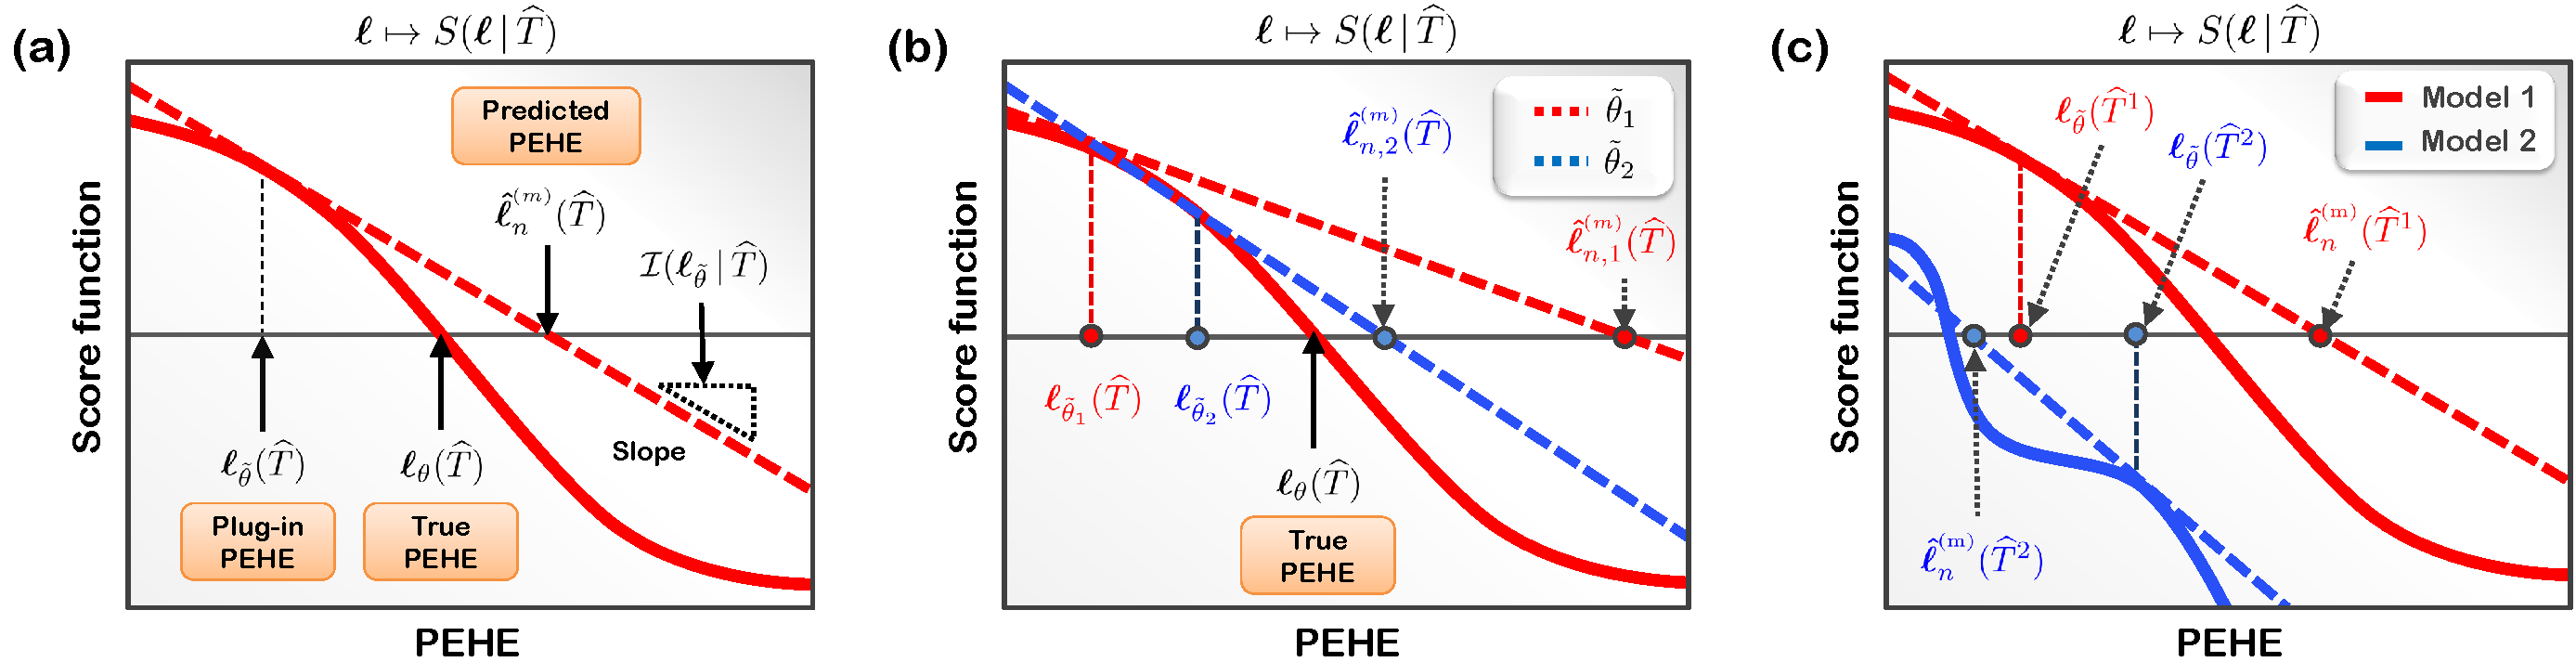
\includegraphics[width=1\linewidth]{ch4Fig3.pdf} 
  \caption{Panels (a)-(c) depict exemplary MLE estimating equations for the PEHE as explained in Section \ref{ch4sec452}. The \mbox{\footnotesize $x$}-axis corresponds to PEHE values (\mbox{\footnotesize $\boldsymbol{\ell}$}), and the \mbox{\footnotesize $y$}-axis corresponds to the score function \mbox{\footnotesize $S(\boldsymbol{\ell}\,|\,\widehat{T})$}. The true PEHE \mbox{\footnotesize $\boldsymbol{\ell}_{\theta}(\widehat{T})$} solves the estimating equation \mbox{\footnotesize $S(\boldsymbol{\ell}\,|\,\widehat{T})=0$}. Solid lines (\rxdash) correspond to \mbox{\footnotesize $S(\boldsymbol{\ell}\,|\,\widehat{T})$}, whereas dashed lines (\rxdashed) depict the derivative of the score at the plug-in PEHE. {\bf (a)} The unplugged validation step is analogous to the first iteration of Fisher scoring via Newton-Raphson method. The predicted PEHE is obtained by correcting for the plug-in bias, which is inversely proportional to the Fisher information metric \mbox{\footnotesize $\mathcal{I}(\boldsymbol{\ell}\,|\,\widehat{T})$}. {\bf (b)} Comparison between two plug-in estimates \mbox{\footnotesize \color{red}{$\tilde{\theta}_1$}} and \mbox{\footnotesize \color{blue}{$\tilde{\theta}_2$}} for a score function \mbox{\footnotesize \color{red}{$S(\boldsymbol{\ell}\,|\,\widehat{T})$}} (\rxdash). The better plug-in estimate conveys more (Fisher) information on the true PEHE, i.e., slope of (\bxdashed) is steeper than that of (\rxdashed), and hence it provides a better PEHE prediction. {\bf (c)} Selecting between two models \mbox{\footnotesize \color{red}{$\widehat{T}^1$}} and \mbox{\footnotesize \color{blue}{$\widehat{T}^2$}} with score functions \mbox{\footnotesize \color{red}{$S(\boldsymbol{\ell}\,|\,\widehat{T}^1)$}} and \mbox{\footnotesize \color{blue}{$S_{\theta}(\boldsymbol{\ell}\,|\,\widehat{T}^2)$}}, respectively. While \mbox{\footnotesize \color{red}{$\widehat{T}^1$}} has a smaller plug-in PEHE than \mbox{\footnotesize \color{blue}{$\widehat{T}^2$}}, predicted PEHEs flip after correcting for plug-in bias.}	
\label{ch4fig3}
\rule{\textwidth}{.75pt}
\end{figure*}
An influence function \mbox{\footnotesize $\boldsymbol{\dot{\ell}}^{\mbox{\tiny $(k)$}}_{\tilde{\theta}}(z_1,.\,.\,.,z_k;\widehat{T})$} can be interpreted as a ``measure of the dependence of \mbox{\footnotesize $\boldsymbol{\ell}_{\tilde{\theta}}$} on the value of \mbox{\footnotesize $k$} data points in the observational data", i.e., its value reflects the sensitivity of the plug-in PEHE estimate to perturbations in the data. Marginalizing out the data \mbox{\footnotesize $(z_1,.\,.\,.,z_k)$} with respect to \mbox{\footnotesize $d(\mathbb{P}_{\theta}-\mathbb{P}_{\tilde{\theta}})$} results in a functional derivative of \mbox{\footnotesize $\boldsymbol{\ell}_{\tilde{\theta}}$} in the ``direction" \mbox{\footnotesize $(\mathbb{P}_{\theta}-\mathbb{P}_{\tilde{\theta}})$} \cite{robins2017minimax}.

The expansion in (\ref{ch4eq15}) represents the plug-in bias $\mbox{\footnotesize $\boldsymbol{\ell}_{\theta}-\boldsymbol{\ell}_{\tilde{\theta}}$}$ in terms of functional derivatives of \mbox{\footnotesize $\boldsymbol{\ell}_{\tilde{\theta}}$}. To see how the bias is captured, consider the first-order von Mises expansion, i.e.,
\begin{align}
\boldsymbol{\ell}_{\theta}(\widehat{T}) \approx \boldsymbol{\ell}_{\tilde{\theta}}(\widehat{T}) + \int \boldsymbol{\dot{\ell}}^{\mbox{\tiny $(1)$}}_{\tilde{\theta}}(z;\widehat{T})\, d(\mathbb{P}_{\theta}-\mathbb{P}_{\tilde{\theta}}). 
\label{ch4eq16}
\end{align}
Thus, the plug-in bias will be large if the functional derivative of \mbox{\footnotesize $\boldsymbol{\ell}_{\tilde{\theta}}$} is large, i.e., the PEHE estimate is sensitive to changes in the plug-in model \mbox{\footnotesize $\tilde{\theta}$}. This derivative will be large if many data points have large influence, and for each such data point, the plug-in distribution is not a good representative of the true distribution, i.e., \mbox{\footnotesize $d(\mathbb{P}_{\theta}-\mathbb{P}_{\tilde{\theta}})$} is large.\\ 
\\
{\bf \mbox{\tiny $\blacksquare$}\,~Dispensing~with~the~counterfactuals.} Note that the expansion in (\ref{ch4eq15}) quantifies the plug-in bias in terms of fixed functions of ``factual" observations \mbox{\footnotesize $Z = (X,W,Y^{\mbox{\tiny $(W)$}})$} only. Thus, the true PEHE can be estimated without knowledge of the counterfactual outcome \mbox{\footnotesize $Y^{\mbox{\tiny $(1-W)$}}$} by calculating the sample average of the first \mbox{\footnotesize $m$} terms of (\ref{ch4eq15}) as follows:
\begin{align}
\boldsymbol{\hat{\ell}}^{\mbox{\tiny $(m)$}}_n(\widehat{T}) = \boldsymbol{\ell}_{\tilde{\theta}}(\widehat{T}) + \sum_{k=1}^m\,\frac{1}{k!}\,\mathbb{U}_{n}\left[\,\boldsymbol{\dot{\ell}}^{\mbox{\tiny $(k)$}}_{\tilde{\theta}}(\boldsymbol{Z};\widehat{T})\,\right], 
\label{ch4eq17}
\end{align} 
where \mbox{\footnotesize $\mathbb{U}_n$} is the empirical \mbox{\footnotesize $U$}-statistic, i.e., the sample average of a multi-input function. (\ref{ch4eq17}) follows directly from (\ref{ch4eq15}) by capitalizing on the unbiasedness of influence functions.

\subsection{Relation to Maximum Likelihood Estimation} 
\label{Sec33}
In Section \ref{ch4sec452}, we used functional calculus to construct a mathematical approximation of a model's performance that does not depend on counterfactual data. But is this approximation also a {\it statistically efficient} estimate?

Recall that in (parametric) maximum likelihood estimation (MLE), a parameter estimate \mbox{\footnotesize $\theta^*$} is obtained by solving the estimating equation \mbox{\footnotesize $S(\theta) = 0$}, where \mbox{\footnotesize $S(\theta)$} is the {\it score} function --- i.e., the derivative of the log-likelihood. For estimating equations that cannot be solved analytically, the classical {\it Fisher scoring} procedure \cite{longford1987fast} is used to obtain a numerical solution for MLE. 

Our two-step validation procedure\footnote{Here we consider a first-order von Mises approximation.} is equivalent to finding the MLE of a model's PEHE using the classical Fisher scoring procedure. To illustrate this equivalence, we capture the structural resemblance between the two procedures in Figure \ref{ch4fig3} as well as the tabulated comparison below. % first order

\begin{center}
\begin{tabular}{ |c|c| } 
\hline
{\bf Estimating equation} & {\bf Fisher scoring} \\
\hline
%& \\ [0.1ex]
(Parametric MLE) & \\
$S(\theta^*) = 0$ & $\hat{\theta} \approx \theta_0 + \,\,\mathcal{I}^{\mbox{\tiny $-1$}}(\theta_0)\,S(\theta_0)$ \\ 
& \\ \hline %[0.05pt] \hline
(Our procedure) & \\
$S(\boldsymbol{\ell}^*\,|\,\widehat{T}) = 0$ & $\boldsymbol{\ell}_{\theta}(\widehat{T}) \approx \boldsymbol{\ell}_{\tilde{\theta}}(\widehat{T}) + \,\,\mathbb{E}_{\theta}[\boldsymbol{\dot{\ell}}^{\mbox{\tiny $(1)$}}_{\tilde{\theta}}(\boldsymbol{z};\widehat{T})]$ \\ 
& \\ %[0.1pt]
\hline
\end{tabular}
\end{center}  

Fisher scoring implements the Newton-Raphson numerical method to solve \mbox{\footnotesize $S(\theta) = 0$}. It utilizes the Taylor approximation of \mbox{\footnotesize $S(\theta)$} around an initial \mbox{\footnotesize $\theta_0$} to formulate an iterative equation \mbox{\footnotesize $\hat{\theta}_{k+1} = \theta^k + \mathcal{I}^{\mbox{\tiny $-1$}}(\theta_k)\,S(\theta_k)$} --- where \mbox{\footnotesize $\mathcal{I}(\theta)$} is the {\it Fisher information} --- that eventually converges to \mbox{\footnotesize $\theta^*$}. From the tabulated comparison above, we can see that our procedure is analogous to the first Newton-Raphson iteration of Fisher scoring. That is, plug-in estimation is similar to finding an initial estimate \mbox{\footnotesize $\theta_0$}, and the unplugged validation step is similar to updating the initial estimate. 

This analogy suggests that our procedure is statistically sound. Similar to cross-validation in supervised learning \cite{dudoit2005asymptotics}, our procedure is a de facto MLE algorithm that computes the ``{most likely PEHE of a model given observational data}". As shown in Figure \ref{ch4fig3}-(a), it does so by searching for the root of the score \mbox{\footnotesize $S(\boldsymbol{\ell}\,|\,\widehat{T})$} via a one-shot Newton-Raphson procedure. 

The juxtaposition of our procedure and Fisher scoring --- in the tabulated comparison above --- suggests an operational definition for Fisher information \mbox{\footnotesize $\mathcal{I}(\boldsymbol{\ell}\,|\,\widehat{T})$} as the ratio between the score function and influence function. (This relation also holds in parametric models \cite{basu1998robust}.) The expression of the plug-in bias in terms of the Fisher metric provides an information-geometric interpretation of our validation procedure. That is, the Fisher information content of the plug-in model \mbox{\footnotesize $\tilde{\theta}$} determines how much the final PEHE estimate will deviate from the initial plug-in estimate (see Figures \ref{ch4fig3}-(b) and \ref{ch4fig3}-(c) for depictions). 

\subsection{Consistency and Efficiency} 
\label{ch4sec454} 
In the following Theorem, we establish the conditions under which our validation procedure is statistically efficient.\\
\\
{\bf Theorem 1.} {\it Let $\mbox{\footnotesize $\mu_0$}$, $\mbox{\footnotesize $\mu_1$}$, and $\mbox{\footnotesize $\pi$}$ be bounded H\"older functions with H\"older exponents $\mbox{\footnotesize $\alpha_0$}$, $\mbox{\footnotesize $\alpha_1$}$ and $\mbox{\footnotesize $\beta$}$, respectively, and $\mbox{\footnotesize $X \in [0,1]^d$}$. If (i) $\mbox{\footnotesize $\widehat{T}$}$ and $\mbox{\footnotesize $\tilde{\theta}$}$ are fit using a separate sample than that used to compute $\mbox{\footnotesize $\boldsymbol{\hat{\ell}}^{\mbox{\tiny $(m)$}}_{n}(\widehat{T})$}$, and (ii) $\mbox{\footnotesize $\widetilde{T}$}$ is a minimax optimal estimate of $\mbox{\footnotesize $T$}$, then we have that:}
\begin{align}
\boldsymbol{\hat{\ell}}^{\mbox{\tiny $(m)$}}_{n}(\widehat{T})-\boldsymbol{\ell}_{\theta}(\widehat{T}) = O_{\mbox{\footnotesize $\mathbb{P}$}}\left(\frac{1}{\sqrt{n}}\vee n^{\frac{-(\alpha_0 \wedge \alpha_1)(m+1)}{2(\alpha_0 \wedge \alpha_1)+d}}\right).  \nonumber
\end{align}
{\it If \mbox{\footnotesize $m \geq \lceil\frac{d}{2(\alpha_0 \wedge \alpha_1)}\rceil$}, then the following is satisfied:} 
\begin{align}
\mbox{\footnotesize {\bf (Consistency)}}& \,\,\,\, \sqrt{n}\,(\boldsymbol{\hat{\ell}}^{\mbox{\tiny $(m)$}}_{n}(\widehat{T})-\boldsymbol{\ell}_{\theta}(\widehat{T})) \overset{d}{\longrightarrow} \mathcal{N}(0,\sigma^2), \nonumber \\
\mbox{\footnotesize {\bf (Efficiency)}}& \,\,\,\, \mbox{Var}[\boldsymbol{\hat{\ell}}^{\mbox{\tiny $(m)$}}_{n}(\widehat{T})] \leq \mbox{Var}[\boldsymbol{\hat{\ell}}^{\prime}(\widehat{T})], \,\,\,\, \nonumber
\end{align}
{\it for some constant $\mbox{\footnotesize $\sigma > 0$}$, and any estimator $\mbox{\footnotesize $\boldsymbol{\hat{\ell}}^{\prime}(\widehat{T})$}$. \,\,\,\,\,\,\,\,\,\,\,\,\,\, $\boldsymbol{\square}$}

This result gives a cut-off value on the minimum number of influence terms $\mbox{\footnotesize $m$}$ needed for the PEHE estimator $\mbox{\footnotesize $\boldsymbol{\hat{\ell}}^{\mbox{\tiny $(m)$}}_{n}(\widehat{T})$}$ to be statistically efficient. This cut-off value depends on the dimensionality and smoothness of the CATE function. 

Theorem 1 also says that the plug-in model $\mbox{\footnotesize $\tilde{\theta}$}$ needs to be good enough for our procedure to work, i.e., $\mbox{\footnotesize $\widetilde{T}$}$ must be a minimax optimal approximation of $\mbox{\footnotesize $T$}$. This is a viable requirement: it is satisfied by models such as Gaussian processes and regression trees \cite{alaa2018limits}.

Finally, Theorem 1 also says that our procedure yields the minimum variance estimator of a model's PEHE. This can be understood in the light of the analogy with MLE (Section \ref{ch4sec452}): since influence functions are proportional to Fisher information, the PEHE estimate in (\ref{ch4eq17}) satisfies the Cram\'er-Rao lower bound on estimation variance. 

\section{Calculating Influence Functions}
\label{ch4sec46} 
Recall that influence functions operationalize the derivatives of \mbox{\footnotesize $\boldsymbol{\ell}_{\theta}(.)$} with respect to distributions induced by \mbox{\footnotesize $\theta$}. But since \mbox{\footnotesize $\mathbb{P}_\theta$} is nonparametric --- i.e., \mbox{\footnotesize $\theta$} is infinite-dimensional --- how can we compute such derivatives? 

A common approach for computing the influence functions of a functional of a nonparametric family \mbox{\footnotesize $\mathcal{P}$} is to define a smooth parametric submodel of \mbox{\footnotesize $\mathcal{P}$}, and then differentiate the functional with respect to the submodel's (scalar) parameter \cite{van2014higher,kennedy2018nonparametric}. A parametric submodel \mbox{\footnotesize $\mathcal{P}_{\varepsilon} = \{\mathbb{P}_{\varepsilon}: \varepsilon \in \mathbb{R}\} \subset \mathcal{P}$} is a subset of models in \mbox{\footnotesize $\mathcal{P}$} that coincides with \mbox{\footnotesize $\mathbb{P}_{\theta}$} at \mbox{\footnotesize $\varepsilon = 0$}. In this Chapter, we choose to work with the following parametric submodel: \mbox{\footnotesize $d\mathbb{P}_{\varepsilon}(z) = (1+\varepsilon h(z))\,d\mathbb{P}_{\theta}(z)$}, for a bounded function \mbox{\footnotesize $h(z)$}. 

Given the submodel \mbox{\footnotesize $\mathbb{P}_{\varepsilon}$}, it can be shown (by manipulating the von Mises series in (\ref{ch4eq17})) that the first order influence function satisfies the following condition: 
\begin{align}  
\frac{\partial\,\boldsymbol{\ell}_{\varepsilon}(\widehat{T})}{\partial \varepsilon}\Big|_{\varepsilon =0} = \mathbb{E}_{\theta}[\,\boldsymbol{\dot{\ell}}^{\mbox{\tiny $(1)$}}_{\theta}(z;\widehat{T})\cdot S_\varepsilon(z)|_{\varepsilon=0}\,],
\label{eq9}
\end{align} 
where \mbox{\footnotesize $S_\varepsilon(z) = \partial \log(d\mathbb{P}_{\varepsilon}(z))/\partial \varepsilon$} is the score function of the parametric submodel, and \mbox{\footnotesize $\boldsymbol{\ell}_{\varepsilon}$} is the PEHE functional evaluated at \mbox{\footnotesize $\mathbb{P}_{\varepsilon}$}. In the next Theorem, we derive a closed-form expression for \mbox{\footnotesize $\boldsymbol{\dot{\ell}}^{\mbox{\tiny $(1)$}}_{\theta}(z;\widehat{T})$}.\\ 
\\
{\bf Theorem 2.} {\it The first order influence function of the PEHE \mbox{\footnotesize $\boldsymbol{\ell}_{\theta}(\widehat{T})$} is unique, and is given by:} 
\begin{align}  
\boldsymbol{\dot{\ell}}^{\mbox{\tiny $(1)$}}_{\theta}(Z;\widehat{T}) =\,\, &(1-B)\,T^2(X) + B\,Y\,(T(X)-\widehat{T}(X)) \, - \nonumber \\
&A\,(T(X)-\widehat{T}(X))^2 + \widehat{T}^2(X) - \boldsymbol{\ell}_{\theta}(\widehat{T}), \nonumber
\end{align} 
{\it where $A = (W-\pi(X))$, and $B = 2W\,(W-\pi(X))\cdot C^{-1}$\,}\\ 
{\it for \mbox{\footnotesize $C = \pi(X)(1-\pi(X))$}.\,\,\,\,\,\,\,\,\,\,\,\,\,\,\,\,\,\,\,\,\,\,\,\,\,\,\,\,\,\,\,\,\,\,\,\,\,\,\,\,\,\,\,\,\,\,\,\,\,\,\,\,\,\,\,\,\,\,\,\,\,\,\,\,\,\,\,\,\,\,\,\,\, $\boldsymbol{\square}$}

This result implies that the influence functions of \mbox{\footnotesize $\boldsymbol{\ell}_{\theta}(\widehat{T})$} do not depend on \mbox{\footnotesize $\eta(x)$}. Thus, the plug-in model \mbox{\footnotesize $\tilde{\theta}$} does not need to be generative. This is a great relief since estimating (high-dimensional) feature distributions can be daunting.

\section{Experiments}
\label{Sec5} 
As envisioned in the beginning of this Chapter, practitioners can use our validation procedure to select the best causal inference method for a given dataset. Unlike pervasive ``expert-driven" modeling practices \cite{rubin2010limitations}, this {\it automated} and data-driven approach to model selection enables confident deployment of (black-box) machine learning-based methods, and safeguards against na\"ive modeling choices.
  
In this Section, we demonstrate the practical significance of influence function-based validation by assessing its utility in model selection. In particular, we assemble a pool of models --- comprising all methods published recently in ICML, NeurIPS and ICLR --- and use our validation procedure to predict the best performing model on 77 benchmark datasets from a recent causal inference competition.

\subsection{Experimental Setup} 
%In what follows, we briefly lay out the experimental setup. Further experimental details are provided in Appendix H.

{\bf \mbox{\tiny $\blacksquare$}\, Influence function-based validation.}\, We implement a stratified \mbox{\footnotesize $P$}-fold version of our validation procedure as follows. First, we randomly split the training data into \mbox{\footnotesize $P$} mutually exclusive subsets, with \mbox{\footnotesize $\mathcal{Z}_p$} being the set of indexes of data points in the \mbox{\footnotesize $p^{th}$} subset, and \mbox{\footnotesize $\mathcal{Z}_{-p}$} its complement. In the \mbox{\footnotesize $p^{th}$} fold, the model being evaluated is trained on the data in \mbox{\footnotesize $\mathcal{Z}_{-p}$}, and issues a CATE estimate \mbox{\footnotesize $\widehat{T}_{-p}$}. For validation, we execute our two-step procedure as follows:\\
\\
\textbf{Step 1: Plug-in estimation}\\
\\
Using~the~dataset~indexed~by~\mbox{\footnotesize $\mathcal{Z}_{-p}$},~we~fit~the~plug-in model \mbox{\footnotesize $\tilde{\theta}_{-p} = \{\tilde{\mu}_{-p,0},\tilde{\mu}_{-p,1},\tilde{\pi}_{-p}\}$} as explained in Section \ref{ch4sec441}. We use two XGBoost regression models for \mbox{\footnotesize $\tilde{\mu}_{-p,0}$} and \mbox{\footnotesize $\tilde{\mu}_{-p,1}$}, and then calculate \mbox{\footnotesize $\widetilde{T}_{-p} = \tilde{\mu}_{-p,1}-\tilde{\mu}_{-p,0}$}. For \mbox{\footnotesize $\tilde{\pi}_{-p}$}, we use an XGBoost classifier. Our choice of XGBoost is motivated by its minimax optimality \cite{linero2018bayesian}, which is required by Theorem 1.\\ 
\\
\textbf{Step 2: Unplugged validation}\\
\\
Given \mbox{\footnotesize $\tilde{\theta}_{-p}$}, we estimate the model's PEHE on the held-out sample \mbox{\footnotesize $\mathcal{Z}_p$} using the estimator in (\ref{ch4eq17}) with \mbox{\footnotesize $m = 1$}, i.e.,
\begin{align}  
\boldsymbol{\hat{\ell}}^{\mbox{\tiny $(1)$}}_p = \sum_{i \in \mathcal{Z}_p}\left[(\widehat{T}_{-p}(X_i)-\widetilde{T}_{-p}(X_i))^2+\boldsymbol{\dot{\ell}}^{\mbox{\tiny $(1)$}}_{\tilde{\theta}_{-p}}(Z_i;\widehat{T}_{-p})\right], \nonumber
\end{align} 
where \mbox{\footnotesize $\boldsymbol{\dot{\ell}}^{\mbox{\tiny $(1)$}}_{\theta}(.)$} is given by Theorem 2. (Here, the first order \mbox{\footnotesize $U$}-statistic \mbox{\footnotesize $\mathbb{U}_1$} in (\ref{ch4eq17}) reduces to a sample average.) The final PEHE estimate is given by the average PEHE estimates over the \mbox{\footnotesize $P$} validation folds, i.e., \mbox{\footnotesize $\boldsymbol{\hat{\ell}}^{\mbox{\tiny $(1)$}}_n = n^{-1}\sum_{p}\boldsymbol{\hat{\ell}}^{\mbox{\tiny $(1)$}}_p$}.\\ 

\begin{table}[t]
\centering %\scalebox{0.9}
%\begin{tcolorbox}[tab3,tabularx={lcc}] %
\begin{tabular}{|lcc|}
\hline
\mbox{\footnotesize \bf Method name} & \mbox{\footnotesize \bf Reference} & \,\,\mbox{\footnotesize \bf $\%$ Winner}\,\,\,\,  \\
\hline
\hline 
{\footnotesize BNN$^{\bigstar}$} & \href{http://proceedings.mlr.press/v48/johansson16.html}{Johansson et al. (2016)} & \,3 $\%$   \\ \hline
{\footnotesize CMGP$^{\ddagger}$} & \href{https://papers.nips.cc/paper/6934-bayesian-inference-of-individualized-treatment-effects-using-multi-task-gaussian-processes.pdf}{Alaa et al. (2017)} &  12 $\%$   \\ \hline
{\footnotesize TARNet$^{\bigstar}$} & \href{http://proceedings.mlr.press/v70/shalit17a.html}{Shalit et al. (2017)} &  \,8 $\%$   \\ \hline
{\footnotesize CFR Wass.$^{\bigstar}$} & \href{http://proceedings.mlr.press/v70/shalit17a.html}{Shalit et al. (2017)} &  12 $\%$  \\ \hline
{\footnotesize CFR MMD$^{\bigstar}$} & \href{http://proceedings.mlr.press/v70/shalit17a.html}{Shalit et al. (2017)} &  \,9 $\%$  \\ \hline
{\footnotesize NSGP$^{\bigstar}$} & \href{http://proceedings.mlr.press/v80/alaa18a.html}{Alaa et al. (2018)} &  17 $\%$   \\ \hline
{\footnotesize GAN-ITE$^{\Diamond}$} & \href{https://openreview.net/forum?id=ByKWUeWA-}{Yoon et al. (2018)} &   \,7 $\%$  \\ \hline
{\footnotesize SITE$^{\ddagger}$} & \href{https://papers.nips.cc/paper/7529-representation-learning-for-treatment-effect-estimation-from-observational-data.pdf}{Yao et al. (2018)} &  \,7 $\%$  \\ \midrule[.025in]
{\footnotesize BART} & \href{https://www.tandfonline.com/doi/abs/10.1198/jcgs.2010.08162}{Hill (2011)} & 15 $\%$  \\ \hline
{\footnotesize Causal Forest} & \href{https://arxiv.org/abs/1510.04342}{Wager et al. (2017)} & 10 $\%$  \\ \midrule[.025in]
{\footnotesize {\bf Factual}} & --- & 53 $\%$  \\ \hline
{\footnotesize {\bf IPTW}} & --- & 54 $\%$ \\ \hline
{\footnotesize {\bf Plug-in}} & --- & 65 $\%$  \\ \hline
{\footnotesize {\bf AutoPrognosis}} & --- & 72 $\%$ \\ \midrule[.025in]
{\footnotesize {\bf Random}} & --- & 10 $\%$  \\ \hline
{\footnotesize {\bf Supervised}} & --- & 84 $\%$ \\ \hline
%\end{tcolorbox}
\end{tabular}
\caption{Comparison of baselines over all datasets.}
\label{ch4Table2}
\end{table}


{\bf \mbox{\tiny $\blacksquare$}\, Automated~causal~inference.}\, Using our validation procedure, we implement the AutoPrognosis BO procedure, and then pick the model with smallest \mbox{\footnotesize $\boldsymbol{\hat{\ell}}^{\mbox{\tiny $(1)$}}_n$}. Our candidate models include all methods published in ICML, NeurIPS and ICLR conferences from 2016 to 2018. This comprises a pool of 8 models, with modeling approaches ranging from Gaussian processes to generative adversarial networks. In addition, we included two other key models developed in the statistics community (BART and causal forests). All candidate models are presented in Table \ref{ch4Table2}.\\
\\
{\bf \mbox{\tiny $\blacksquare$}\, Data~description.}\,~We~conducted~extensive~experiments on benchmark datasets released by the ``Atlantic Causal Inference Competition" \cite{HillACIC}, a data analysis competition that compared models of treatment effects. The competition involved 77 semi-synthetic datasets: all datasets shared the same data on features \mbox{\footnotesize $X$}, but each dataset had its own simulated outcomes and assignments \mbox{\footnotesize $(W,Y)$}. Features were extracted from a real-world observational study, whereas outcomes and assignments were simulated via data generating processes that were carefully designed to mimic real data. Each of the 77 datasets had a unique data generating process encoding varying properties (e.g., levels of treatment effect heterogeneity, dimensionality of the relevant feature space, etc.) Detailed explanation of the data generating processes was published by the organizers of the competition in \cite{dorie2017automated}. %An in-depth description of the released data is provided in Appendix H.    

The feature data shared by all datasets was extracted from the Collaborative Perinatal Project \cite{niswander1972collaborative}, a study conducted on a cohort of pregnant women to identify causes of infants' developmental disorders. The treatment was a child's birth weight (\mbox{\footnotesize $W = 1$} if weight \mbox{\footnotesize $<$} 2.5 \mbox{\footnotesize $kg$}), and outcome was the child's IQ after a given follow-up period. The study contained 4,802 data points with 55 features (5 are binary, 27 are count data, and 23 are continuous).\\
\\
{\bf \mbox{\tiny $\blacksquare$}\,~Performance~evaluation.}\,~We~applied~automated~causal inference~on~10~realizations~of~the~simulated~outcomes~for each of the 77 datasets, i.e., a total of 770 replications. (Those realizations were generated by the competition organizers and are publicly accessible \cite{HillACIC}.) For each realization, we divide the data into 80/20 train/test splits, and use training data to predict the PEHE of the 10 candidate models via 5-fold influence function-based validation. Then, we select the model with smallest estimated PEHE, and evaluate its PEHE on the out-of-sample testing data.\\ 
\\
{\bf \mbox{\tiny $\blacksquare$}\,~Baselines.}\,~We~compare~influence~function-based~validation with 3 heuristics commonly used in the epidemiological and statistical literature \cite{schuler2018general}:

\setlength\arrayrulewidth{0.7pt}
\begin{center}
\begin{tabular}{ |c|l| }
\hline
\cellcolor{red!6}\mbox{\footnotesize {\bf Baseline}} & \cellcolor{red!6}\,\,\,\,\,\,\,\,\,\,\,\,\,\,\,\,\,\,\,\,\,\,\,\mbox{\footnotesize {\bf PEHE estimator}} \\ 
\hline
\cellcolor{red!3}& \\
\cellcolor{red!3}\mbox{\footnotesize {\bf Factual validation}} & \mbox{\footnotesize $\boldsymbol{\hat{\ell}}_n(\widehat{T}) = \frac{1}{n}\sum_{i}(\hat{\mu}_{{\mbox{\tiny $W_i$}}}(X_i)-Y_i^{\mbox{\tiny $(W_i)$}})^2$} \\[10pt] 
\cellcolor{red!3}\mbox{\footnotesize {\bf IPTW validation}} & \mbox{\footnotesize $\boldsymbol{\hat{\ell}}_n(\widehat{T}) = \frac{1}{n}\sum_{i}\frac{(\hat{\mu}_{{\mbox{\tiny $W_i$}}}(X_i)-Y_i^{\mbox{\tiny $(W_i)$}})^2}{(1-2W_i)(1-W_i-\tilde{\pi}(X_i))}$} \\[10pt]
\cellcolor{red!3}\mbox{\footnotesize {\bf Plug-in validation}} & \mbox{\footnotesize $\boldsymbol{\hat{\ell}}_n(\widehat{T}) = \frac{1}{n}\sum_{i}(\widehat{T}(X_i)-\widetilde{T}(X_i))^2$} \\ 
\cellcolor{red!3}& \\
\hline
\end{tabular}
\end{center}
Factual validation evaluates the error in the potential outcomes \mbox{\footnotesize $(\mu_0,\mu_1)$} using factual samples only. Inverse propensity weighted (IPTW) validation is similar, but weights each sample with its (estimated) ``propensity score" \mbox{\footnotesize $\tilde{\pi}(x)$} to obtain unbiased estimates \cite{van2003unified}. Plug-in validation is identical to Step 1 of our procedure: it obtains a plug-in PEHE estimate \cite{rolling2014model,schuler2017synth}. To ensure fair comparisons, we model \mbox{\footnotesize $\widetilde{T}$} and \mbox{\footnotesize $\widetilde{\pi}$} in the heuristics above using XGBoost models similar to the ones used in Step 1 of our procedure.\\
\\
{\bf \mbox{\tiny $\blacksquare$}\, Results.}\, Table \ref{ch4Table2} summarizes the fraction of datasets for which each baseline comes out as winner across all datasets\footnote{The magnitudes of causal effects were not consistent across datasets, hence PEHE values were in different numerical ranges.}. As we can see, our influence function-based (IF-based) approach that automatically picks the best model for every dataset outperforms any single model applied repeatedly to all datasets. This is because the 77 datasets encode different data generating processes, and hence no single model is expected to be a good fit for all datasets. The gains achieved by automation are substantial --- the PEHE of the automated approach was (on average) 47\% smaller than that of the best performing single model. 

It comes as no surprise that our procedure outperforms the factual, IPWT and plug-in validation heuristics. This is because, as we have shown in Theorem 1, the IF-based approach is the most efficient estimator of PEHE. We also compare our validation procedure with the ``supervised" cross-validation procedure that is allowd to observe the counterfactual data in the training set. As we can see, despite having access to less information, our IF-based approach comes closer to the supervised approach (as compared to the competing validation methods). 


\chapter{Deep Probabilistic Modeling of Longitudinal Data}

Chronic diseases --- such as cardiovascular disease, cancer and diabetes --- progress slowly throughout a patient's lifetime, causing increasing burden to the patients, their carers, and the healthcare delivery system \cite{sevick2007patients}. The advent of modern electronic health records (EHR) provides an opportunity for building models of disease progression that can \textit{predict} individual-level disease trajectories, and distill \textit{intelligible} and \textit{actionable} representations of disease dynamics \cite{blumenthal2010meaningful}. Models that are both highly accurate and capable of extracting knowledge from data are important for informing practice guidelines and identifying the patients' needs and interactions with health services \cite{topol2019high,coyne2011management,valderas2009defining}. 

In this Chapter, we develop a deep probabilistic model of disease progression that capitalizes on both the interpretable structured representations of probabilistic models and the predictive strength of deep learning methods. Unlike the previous Chapters, here we address the longitudinal data setup where follow-up data are collected for the same patient over time. Our model uses a state-space representation to segment a patient's disease trajectory into ``stages'' of progression that manifest through clinical observations. But unlike conventional state-space models, which are predominantly Markovian, our model uses recurrent neural networks (RNN) to capture more complex state dynamics. The proposed model learns hidden disease states from observational data in an unsupervised fashion, and hence it is suitable for EHR data where a patient's record is seldom annotated with ``labels'' indicating their true health state \cite{alaa2016hidden}.

\begin{figure*}[t!] 
    \centering
    \begin{subfigure}[t]{0.32\textwidth}
        \centering
        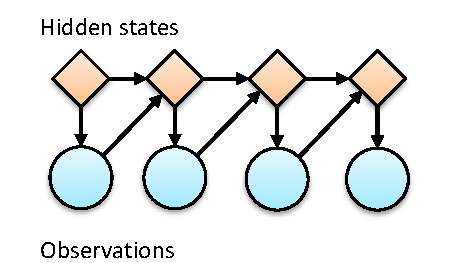
\includegraphics[width=1.85in]{ch5Fig1b.pdf}
        \caption{\footnotesize RNN}
				\label{fig1a}
    \end{subfigure}%
    ~ 
    \begin{subfigure}[t]{0.32\textwidth}
        \centering
        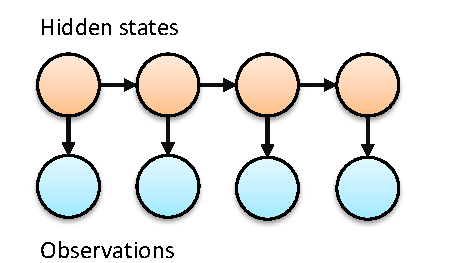
\includegraphics[width=1.85in]{ch5Fig1a.pdf}
        \caption{\footnotesize HMM}
				\label{fig1b}
    \end{subfigure}
		 ~ 
    \begin{subfigure}[t]{0.32\textwidth}
        \centering
        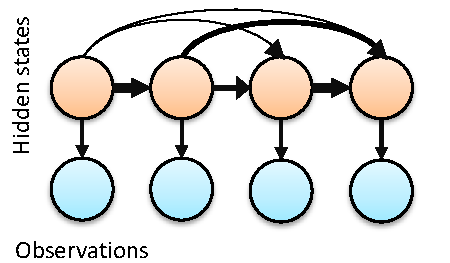
\includegraphics[width=1.85in]{ch5Fig1c.pdf}
        \caption{\footnotesize Attentive state space}
				\label{fig1c}
    \end{subfigure}
    \caption{{\bf Sequential data models.} (a) Graphical model for an RNN. $\Diamond$ denotes a deterministic representation, (b) Graphical model for an HMM. $\bigcirc$ denotes probabilistic states, (c) Graphical depiction of an attentive state space model. With a slight abuse of graphical model notation, thickness of arrows reflect attention weights.}
\end{figure*}

Our model uses an {\it attention} mechanism to capture state dynamics, hence we call it an {\it attentive state-space} model. The attention mechanism observes the patient's clinical history, and maps it to attention weights that determine how much influence previous disease states have on future state transitions. In that sense, attention weights generated for an individual patient explain the causative and associative relationships between the hidden disease states and the past clinical events for that patient. Because the attention mechanism can be made arbitrarily complex, our model can capture complex dynamics while maintaining its structural interpretability. We implement this dynamic attention mechanism via a sequence-to-sequence RNN architecture \cite{sutskever2014sequence}.  

Because our model is non-Markovian, inference of posterior disease states is intractable and cannot be conducted using standard forward-backward routines (e.g., \cite{liu2015efficient,dai2016recurrent,zheng2017state}). To address this issue, we devise a structured inference network trained to predict posterior state distributions by mimicking the attentive structure of our model. The inference network shares attention weights with the generative model, and uses those weights to create summary statistics needed for posterior inference. We jointly train the inference and model networks using stochastic gradient descent.

To demonstrate the practical significance of the attentive state-space model, we use it to model the progression trajectories of breast cancer using data from the UK Cystic Fibrosis registry. Our experiments show that attentive state-space models can extract clinically meaningful representations of disease progression while maintaining superior predictive accuracy for future outcomes. 

\section{Related Literature}

Various predictive models based on RNNs have been recently developed for healthcare settings --- e.g., ``Doctor AI'' \cite{choi2016doctor}, ``L2D'' \cite{lipton2015learning}, and ``Disease-Atlas'' \cite{lim2018disease}. Unfortunately, RNNs are of a ``black-box'' nature since their hidden states do not correspond to clinically meaningful variables (Figure \ref{fig1a}). Thus, all the aforementioned methods do not provide an intelligible model of disease progression, but are rather limited to predicting a target outcome.  

There have been various attempts to create interpretable RNN-based predictive models using attention. The models in \cite{choi2016retain,ma2017dipole,kwon2019retainvis} use a reverse-time attention mechanism to learn visit-level attention weights that explain the predictions of an RNN. The main difference between the way attention is used in our model and the way it is used in models like ``RETAIN'' \cite{choi2016retain} is that our model applies attention to the latent {\it state space}, whereas RETAIN applies attention to the observable {\it sample space}. Hence, attention gives different types of explanations in the two models. In our model, attention interprets the hidden disease dynamics, hence it provides an explanation for the mechanisms underlying disease progression. On the contrary, RETAIN uses attention to measure feature importance, hence it can only explain discriminative predictions, but not the underlying generative disease dynamics.  

Almost all existing models of disease progression are based on variants of the HMM model \cite{wang2014unsupervised,liu2015efficient,alaa2017learning}. Disease dynamics in such models are very easily interpretable as they can be perfectly summarized through a single matrix of probabilities that describes transition rates among disease states. Markovian dynamics also simplify inference because the model likelihood factorizes in a way that makes efficient forward and backward message passing possible. However, memoryless Markov models assume that a patient's current state $d$-separates her future trajectory from her clinical history (Figure \ref{fig1b}). This renders HMM-based models incapable of properly explaining the heterogeneity in the patients' progression trajectories, which often results from their varying clinical histories or the chronologies (timing and order) of their clinical events \cite{valderas2009defining}. This limitation is crucial in complex chronic diseases that are accompanied with multiple morbidities. Our model addresses this limitation by creating memoryful state transitions that depend on the patient's entire clinical history (Figure \ref{fig1c}).

Most existing works on deep probabilistic models have focused on developing structured inference algorithms for deep Markov models and their variants \cite{krishnan2017structured,dai2016recurrent,karl2016deep,johnson2016composing,rangapuram2018deep}. All such models use neural networks to model the transition and emission distributions, but are limited to Markovian dynamics. Other works develop stochastic versions of RNNs for the sake of generative modeling; examples include variational RNNs \cite{chung2015recurrent}, SRNN \cite{fraccaro2016sequential}, and STORN \cite{bayer2014learning}. These models augment stochastic layers to an RNN in order to enrich its output distribution. However, transition and emission distributions in such models cannot be decoupled, and hence their latent states do not map to clinically meaningful identification of disease states. To the best of our knowledge, ours~is~the first deep probabilistic model that provides clinically meaningful latent representations,~with~non-Markovian state dynamics that can be made arbitrarily complex while remaining interpretable.

\section{Attentive State-Space Models}
\label{ch5sec2}
We start off by describing the structure of EHR data in Section \ref{ch5sec21}, and then we develop the attentive state-space representation of disease progression in Section \ref{ch5sec22}.  

\subsection{Structure of the EHR Data}
\label{ch5sec21}
A~patient's~EHR~record,~denoted~as~$\boldsymbol{\vec{x}}_T$,~is~a~collection~of~sequential follow-up data gathered during repeated hospital visits. We represent a given patient's record as  
\begin{equation}
\boldsymbol{\vec{x}}_T = \{x_{t}\}^{T}_{t=1}, 
\label{ch5eq1}
\end{equation}    
where $x_{t}$ is the follow-up data collected during the $t^{th}$ hospital visit, and $T$ is the total number of visits. The follow-up data $x_{t} \in \mathcal{X}$ is a multi-dimensional vector that comprises information on biomarkers and clinical events, such as treatments and ICD-10 diagnosis codes \cite{blumenthal2010meaningful}. 

\subsection{Attentive State-Space Representation}
\label{ch5sec22}
We model the progression trajectory of the target disease via a state-space representation. That is, at each time step $t$, the patient's health is characterized by a state $z_t \in \mathcal{Z}$ which manifests through the follow-up data $x_t$. The state space is the (discrete) set of all possible stages of disease progression $\mathcal{Z} = \{1,.\,.\,.\,,K\}$. In general, progression stages correspond to distinct disease  phenotypes. For instance, chronic kidney disease progresses through 5 stages (Stage I to Stage IV), each of which corresponds to a different level of renal dysfunction \cite{eddy2006chronic}. We assume that $\{z_t\}_{t}$ is {\it hidden}, i.e., the true health state of a patient is not observed, and should be learned in an unsupervised fashion. We model the joint distribution of states and observations via the following factorization: 
\begin{align}
p_{\theta}(\boldsymbol{\vec{x}}_T, \boldsymbol{\vec{z}}_T) = \prod^{T}_{t=1}\,\, \underbrace{p_{\theta}(x_{t}\,|\,z_{t})}_{\mbox{\footnotesize {\bf Emission}}}\,\,\underbrace{p_{\theta}(z_{t}\,|\,\boldsymbol{\vec{x}}_{t-1}, \boldsymbol{\vec{z}}_{t-1})}_{\mbox{\footnotesize {\bf Transition}}}, 
\label{ch5eq2}
\end{align}
where $\boldsymbol{\vec{z}}_t = \{z_1,.\,.\,.,z_t\},\, 1 \leq t \leq T$, and $\theta$ is the set of parameters of our model.\\ 
\\
{\bf Attentive state transitions.} What makes the~model~in~(\ref{ch5eq2}) differ from standard~state-space~models? The main difference is that the transition probability in (\ref{ch5eq2}) assumes that the patient's health state at time $t$ depends on their entire history $(\boldsymbol{\vec{x}}_{t-1}, \boldsymbol{\vec{z}}_{t-1})$. This is a major departure from the standard Markovian assumption, which posits that $p_{\theta}(z_{t}\,|\,\boldsymbol{\vec{x}}_{t-1}, \boldsymbol{\vec{z}}_{t-1}) = p_{\theta}(z_{t}\,|\,z_{t-1})$, i.e., future states depend only on current state. Most existing disease models are Markovian (e.g., \cite{liu2015efficient,wang2014unsupervised}).

To capture non-Markovian dynamics, we model the state transition distribution as follows: 
\begin{align}
p_{\theta}(z_{t}\,|\,\boldsymbol{\vec{x}}_{t-1}, \boldsymbol{\vec{z}}_{t-1}) = p_{\theta}(z_{t}\,|\,\boldsymbol{\vec{\alpha}}_{t}, \boldsymbol{\vec{z}}_{t-1}),
\label{ch5eq3}
\end{align}
where $\boldsymbol{\vec{\alpha}}_{t} = \{\alpha^t_1,.\,.\,.,\alpha^t_{t-1}\}$, $\alpha^t_i \in [0,1], \forall i$, $\sum_{i} \alpha^t_i = 1$, is a set of {\it attention weights} that act as sufficient statistics of future states. The attention weights admit to a simple interpretation: they determine the influences of past state realizations on future state transitions via the linear dynamic
\begin{align}
p_{\theta}(z_{t}\,|\,\boldsymbol{\vec{\alpha}}_{t}, \boldsymbol{\vec{z}}_{t-1}) = \sum^{t-1}_{t^{\prime}=1} \alpha^{t-1}_{t^{\prime}}\,\boldsymbol{P}(z_{t^{\prime}},z_{t}),\, \forall t \geq 1,
\label{ch5eq4}
\end{align}
where $\boldsymbol{P}$ is a baseline state transition matrix, i.e., $\boldsymbol{P} = \,\mbox{\footnotesize $p_{\mbox{\tiny $ij$}} \in [0,1],\, \sum_{j}p_{\mbox{\tiny $ij$}} = 1$},$ and the initial state distribution is $\boldsymbol{\pi} = [\,p_{\mbox{\tiny $1$}},.\,.\,.,p_{\mbox{\tiny $K$}}\,].$ The attention weights $\boldsymbol{\vec{\alpha}}_{t}$ assigned to all previous state realizations at time $t$ are generated using the patient's {\it context} $\boldsymbol{\vec{x}}_t$ via an attention mechanism $\boldsymbol{A}$ as follows: 
\begin{align}
\boldsymbol{\vec{\alpha}}_{t} = A_t(\boldsymbol{\vec{x}}_{t}). 
\label{ch5eq5}
\end{align}
where $\boldsymbol{A}$ is a deterministic algorithm that generates a sequence of functions $\{A_t\}_t$, $A_t:\mathcal{X}^t \to [0,1]^t$. We specify our choice of the attention mechanism in the next Section.\\ 
\\
{\bf Emission distribution.} The follow-up data $x_t = (x^c_{t},x^b_{t})$ comprises both a continuous component $x^c_{t}$ (e.g., biomarkers and test results) and a binary component $x^b_{t}$ (e.g., clinical events and ICD-10 codes). To capture both components, we model the emission distribution in (\ref{ch5eq2}) through the following factors $p_{\theta}(x_{t}\,|\,z_{t}) = p_{\theta}(x^b_{t}\,|\,x^c_{t},z_{t})\cdot p_{\theta}(x^c_{t}\,|\,z_{t})$, where
\begin{align}
p_{\theta}(x^c_{t}\,|\,z_{t}) = \mathcal{N}(\mu_{z_{t}},\Sigma_{z_{t}}),\,\,\,\, 
p_{\theta}(x^b_{t}\,|\,x^c_{t},z_{t}) = \mbox{Bernoulli}(\mbox{Logistic}(x^c_{t},\Lambda_{z_{t}})). 
\label{ch5eq6}
\end{align}   

The model in (\ref{ch5eq6}) specifies a state-specific distribution for binary (Bernoulli) and continuous (Gaussian) variables, with state-specific emission distribution parameters $(\mu_{z_{t}},\Sigma_{z_{t}},\Lambda_{z_{t}})$. This, an attentive state-space model is completely specified through $\theta = (\boldsymbol{\pi},\boldsymbol{P},\boldsymbol{A},\boldsymbol{\mu},\boldsymbol{\Sigma},\boldsymbol{\Lambda})$.\\
\\
{\bf Generality of the attentive representation.}\,\,For particular choices of the attention mechanism in (\ref{ch5eq5}), our model reduces to various classical models of sequential data as shown in Table \ref{ch5Table1}. The generality of the attentive state representation is a powerful feature because it implies that by learning the attention functions $\{A_t\}_t$, we are effectively testing the structural assumptions of various commonly-used time series models in a data-driven fashion. 

\begin{table}
\centering 
\begin{tabular}{cc}
    \toprule
    {\footnotesize \bf Model} & {\footnotesize \bf Attention mechanism}  \\
    \midrule
    {\footnotesize {\bf HMM} \cite{liu2015efficient}} & \mbox{\footnotesize $\alpha^t_{t-1} = 1, \alpha^t_j = 0,\, j \leq t-2$.}  \\[1ex]
    {\footnotesize {\bf Order-$m$ HMM} \cite{willems1995context}} & \mbox{\footnotesize $\alpha^t_j = \boldsymbol{1}_{\{m \leq j \leq t-1\}},\, j \leq t-2$.} \\[1ex]
    {\footnotesize {\bf Variable-order HMM} \cite{begleiter2004prediction}} & \mbox{\footnotesize $\alpha^t_j \in \{0,\bar{n}^{-1}\}, \bar{n} = \sum_i\boldsymbol{1}_{\{\alpha^t_i \geq \gamma\}}$.} \\
    \bottomrule  
  \end{tabular}
  \caption{Reduction of attentive state-space models to standard models.}
  \label{ch5Table1}
\end{table}

\subsection{Sequence-to-sequence Attention Mechanism}
\label{SSec23} 
To complete the specification of our model, we now specify the attention mechanism $\boldsymbol{A}$ in (\ref{ch5eq5}). Recall that $\boldsymbol{A}$ is a sequence of deterministic functions that map a patient's context $\boldsymbol{\vec{x}}_t$ to a set of attention weights $\boldsymbol{\vec{\alpha}}_{t}$ at each time step. Since our model must output an entire sequence of attention weights every time step, we implement $\boldsymbol{A}$ via a sequence-to-sequence (Seq2Seq) model \cite{sutskever2014sequence}. 

Our Seq2Seq model uses LSTM encoder-decoder architecture as shown in Figure \ref{ch5fig2}. For each time step $t$, the patient context $\boldsymbol{\vec{x}}_t$ is fed to the LSTM encoder, and the final state of the encoder, $\boldsymbol{h}_t$, is viewed as a fixed-size representation of the patient's context, and is passed together with the last output $O$ to the decoder side. 

\begin{figure}[h]
\centering
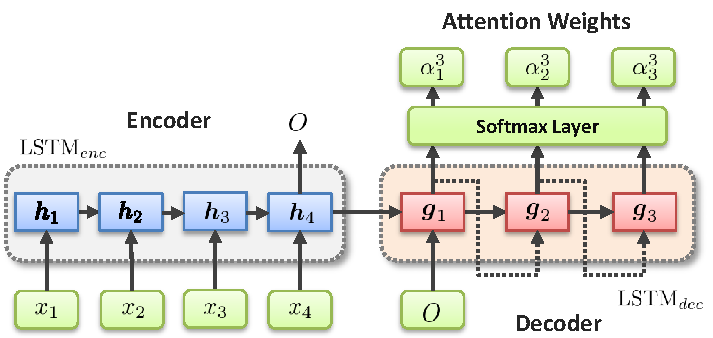
\includegraphics[width=4.75in]{ch5Fig2.pdf}
\caption{Seq2Seq architecture for the attention mechanism $\boldsymbol{A}$.}
\label{ch5fig2}
\end{figure}

In the decoding phase, the last state of the encoding LSTM is used as an initial state of the decoding LSTM, and $O$ is used as its first input. Then, the decoding LSTM iteratively uses its output at one time step as its input for the next step. After $t-1$ decoding iterations, we collect the $t-1$ (normalized) attention weights via a Softmax output layer.  

The main difference between our architecture and other Seq2Seq models --- often used in language translation tasks \cite{bahdanau2014neural,sutskever2014sequence} --- is that in our case, we learn an entire sequence of attention weights for each of the $T$ data vectors in $\boldsymbol{\vec{x}}_{T}$. We achieve this by running $t-1$ decoding iterations to collect $t-1$ outputs for every single encoding step. Moreover, in our setup attention sequence is the target sequence being learned. This should not be confused with other Seq2Seq schemes with attention, where attention is used as an intermediate representation within the decoder \cite{vaswani2017attention}. 

\subsection{Why Attentive State Space Modeling?} %example supplement 
\label{ch5sec24}
Most existing models of disease progression are based on Hidden Markov models \cite{alaa2017learning,liu2015efficient,wang2014unsupervised,green2002hidden}. However, the Markovian dynamic is oversimplified: in reality, a patient transition to a given state depends not only on her current stage, but also on her individual history of past clinical events \cite{sevick2007patients}. In this sense, a Markov models is of a ``one-size-fits-all'' nature --- under a Markov model, all patients at the same stage of progression would have the same expected future trajectory, irrespective of their potentially different individual clinical histories. Because Markov models explain away individual-level variations in progression trajectories, their interpretable nature should be thought of as a bug and not a feature, i.e., a Markov model is easily interpretable only because it {\it does not explain much}, it only encodes our own prior assumptions about disease dynamics. 

Attentive state space models overcome the shortcomings of Markov models by using attention weights to create non-stationary, variable-order generalization of Markovian transitions, whereby the dynamics of each patient changes over time based on her {\it individual} clinical context. An attentive state model can learn dynamics that are as complex as those of an RNN, but through the factorization in (\ref{ch5eq2}), it ensures that its hidden states correspond to meaningful disease states. 

\section{Attentive Variational Inference}
\label{ch5sec3}
Learning the model parameter $\theta$ and inferring a patient's health state in real-time requires computing the posterior $p_{\theta}(\boldsymbol{\vec{z}}_t\,|\,\boldsymbol{\vec{x}}_t)$. However, the non-Markovian nature of our model renders posterior computation intractable. In this Section, we develop a variational learning algorithm that jointly learns the model parameter $\theta$ and a structured inference network that approximates the posterior $p_{\theta}(\boldsymbol{\vec{z}}_t\,|\,\boldsymbol{\vec{x}}_t)$. We show that the attentive representation proposed is useful not only for improving predictions and extracting clinical knowledge, but also can help improve structured inference. 

\subsection{Variational Lower Bound}
\label{ch5sec31}
In variational learning, we maximize an evidence lower bound (ELBO) for the data likelihood, i.e., 
\begin{align}
\log p_{\theta}(\boldsymbol{\vec{x}}_{T}) \geq \mathbb{E}_{q_{\phi}} \left[\, \log p_{\theta}(\boldsymbol{\vec{x}}_{T},\boldsymbol{\vec{z}}_{T}) - \log q_{\phi}(\boldsymbol{\vec{z}}_{T}\,|\,\boldsymbol{\vec{x}}_{T}) \,\right], \nonumber 
%\label{eq101}
\end{align}
where $q_{\phi}(\boldsymbol{\vec{z}}_{T}\,|\,\boldsymbol{\vec{x}}_{T})$ is a variational distribution that approximates the posterior $p_{\theta}(\boldsymbol{\vec{z}}_{T}\,|\,\boldsymbol{\vec{x}}_{T})$. We model the variational distribution $q_{\phi}(\boldsymbol{\vec{z}}_{T}\,|\,\boldsymbol{\vec{x}}_{T})$ using an {\it inference network} that is trained jointly with the model through the following optimization problem \cite{mnih2014neural,kingma2013auto}:
\begin{align}
\theta^*, \phi^* \ = \arg \max_{\theta, \phi}\, \mathbb{E}_{q_{\phi}} \left[\,\log p_{\theta}(\boldsymbol{\vec{x}}_{T},\boldsymbol{\vec{z}}_{T}) - \log q_{\phi}(\boldsymbol{\vec{z}}_{T}\,|\,\boldsymbol{\vec{x}}_{T}) \,\right]. 
\label{ch5eq7}
\end{align}
By estimating $\theta$ and $\phi$ from the EHR data, we recover the generative model $p_{\theta}(\boldsymbol{\vec{x}}_{T},\boldsymbol{\vec{z}}_{T})$,~through which we can extract clinical knowledge, and the inference network $q_{\phi}(\boldsymbol{\vec{z}}_{T}\,|\,\boldsymbol{\vec{x}}_{T})$, through which we can use to infer the health trajectory of the patient at hand.

\subsection{Attentive Inference Network} % Get the structure of the posterior, network structure
\label{ch5sec32}
We construct the inference network $q_{\phi}(\boldsymbol{\vec{z}}_{T}\,|\,\boldsymbol{\vec{x}}_{T})$ so that it mimics the structure of the true posterior \cite{krishnan2017structured}. Recall that the posterior factorizes as follows:
\begin{align}
p_{\theta}(\boldsymbol{\vec{z}}_T\,|\,\boldsymbol{\vec{x}}_T) = p_{\theta}(z_1\,|\,\boldsymbol{\vec{x}}_T) \prod^{T}_{t=2} p_{\theta}(z_t\,|\,\boldsymbol{\vec{\alpha}}_{t-1},\boldsymbol{\vec{z}}_{t-1},\boldsymbol{\vec{x}}_{t:T}). \nonumber 
%\label{eq100}
\end{align}
Consequently, we impose a similar factorization on the inference network, i.e., 
\begin{align}
q_{\phi}(\boldsymbol{\vec{z}}_T\,|\,\boldsymbol{\vec{x}}_T) = q_{\phi}(z_1\,|\,\boldsymbol{\vec{x}}_T) \prod^{T}_{t=2} q_{\phi}(z_t\,|\,\boldsymbol{\vec{\alpha}}_{t-1},\boldsymbol{\vec{z}}_{t-1},\boldsymbol{\vec{x}}_{t:T}). 
\label{ch5eq8}
\end{align}

To capture the factorization in (\ref{ch5eq8}), we use the architecture in Figure \ref{ch5fig3} to construct an inference network that mimics the attentive structure of the generative model. In this architecture, a ``combiner function'' $\boldsymbol{C}(.)$ is fed with all the sufficient statistics of a state $z_t$, and outputs its posterior distribution. The combiner uses the attention weights created by $\boldsymbol{A}$ to condense summary statistics of $z_t$.  

As dictated by (\ref{ch5eq8}), the parent nodes of $z_t$ are the attention weights $\boldsymbol{\vec{\alpha}}_{t}$, the previous states $\boldsymbol{\vec{z}}_{t-1}$ and the future observations $\boldsymbol{\vec{x}}_{t:T}$. The inference network encodes these sufficient statistics as follows. The attention weights $\boldsymbol{\vec{\alpha}}_{t}$ are shared with the attention network in Figure \ref{ch5fig2}. The future observations $\boldsymbol{\vec{x}}_{t:T}$ are summarized at time $t$ via a backward LSTM that reads $\boldsymbol{\vec{x}}_{T}$ in a reversed order as shown in Figure \ref{ch5fig3}. Finally, the previous states $\boldsymbol{\vec{z}}_{t-1}$ are sampled from the combiner functions at previous time steps as described below.\\ 
\\
{\bf Posterior sampling.}\, In order to sample posterior state trajectories from the inference network, we iterate over the combiner function $\boldsymbol{C}(.)$ for $t \in \{1,.\,.\,.,T\}$ as follows:
\begin{align}
\boldsymbol{\tilde{p}}_t &= C(\boldsymbol{h}^t_q,\boldsymbol{\vec{\alpha}}_{t},(\tilde{z}_1,.\,.\,.,\tilde{z}_{t-1})\,|\,\boldsymbol{\pi},\boldsymbol{P}),\nonumber\\
\tilde{z}_t        &\sim \mbox{Multinomial}(\boldsymbol{\tilde{p}}_t),
\label{ch5eq9}
\end{align}
where $\boldsymbol{\tilde{p}}_t = (\tilde{p}^t_1,.\,.,\,.,\tilde{p}^t_K), \sum_k \tilde{p}^t_k =1$, is the posterior state distribution estimated by the inference network at time $t$, and $\boldsymbol{h}^t_q$ is the $t^{th}$ state of the backward LSTM in Figure \ref{ch5fig3}, which summarizes the information in $\boldsymbol{\vec{x}}_{t:T}$. As we can see in (\ref{ch5eq9}), at each time step $t$, the combiner function takes as an input {\it all} the previous states $(\tilde{z}_1,.\,.\,.,\tilde{z}_{t-1})$ sampled by earlier executions of the combiner function. The dashed blue lines in Figure 3 depict the passage of older state samples to later executions of the combiner function. 

\begin{figure}[t]
\centering
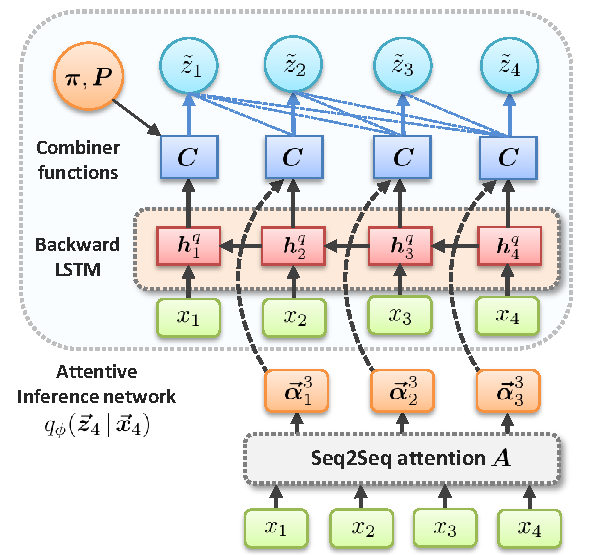
\includegraphics[width=3.75in]{ch5Fig3.pdf}
\caption{Attentive inference network.}
\label{ch5fig3}
\end{figure}

The combiner function estimates the posterior $\boldsymbol{\tilde{p}}_t$ by emulating the state transition model in (\ref{ch5eq5}), i.e.,
\begin{align} 
\tilde{p}^t_{k, forward}         &= \mbox{\footnotesize $\sum^{t-1}_{t^{\prime}=1}$}\alpha_{t^{\prime}}^t\boldsymbol{P}(\tilde{z}_{t^{\prime}},k),\, k \in \{1,.\,.\,.,K\},	\nonumber \\
\boldsymbol{\tilde{h}}^t_q &= [\boldsymbol{h}^t_q,\tilde{p}^t_{1, forward}.\,.\,.,\tilde{p}^t_{K, forward}], \nonumber \\
\boldsymbol{\tilde{p}}_t &= \mbox{Softmax}(\boldsymbol{W}_{q}^\top \tilde{\boldsymbol{h}}^t_q + b_q).
\label{ch5eq10}
\end{align}
As shown in (\ref{ch5eq10}), the combiner emulates the generative model to compute an estimate of the ``filtering'' distribution $\tilde{p}^t_{k, forward} \approx p_{\theta}(z_t\,|\,\boldsymbol{\vec{x}}_t)$, i.e., it attends to previously sampled states with proportions determined by the attention weights. Then, to augment information from the future observations $\boldsymbol{\vec{x}}_{t:T}$, it concatenates the filtering distribution with the backward LSTM state and estimates the posterior through a Softmax output layer.

\subsection{Learning with Stochastic Gradient Descent} 
\label{ch5sec33}
In order to simultaneously learn the parameters of the generative model and inference network, we use stochastic gradient descent to solve (\ref{ch5eq10}) as follows: 

\begin{enumerate} 
\itemsep0em 
\item Sample $(\tilde{z}^{\mbox{\tiny $(i)$}}_1,.\,.\,.,\tilde{z}^{\mbox{\tiny $(i)$}}_T) \sim q_{\phi}(\boldsymbol{\vec{z}}_{T}\,|\,\boldsymbol{\vec{x}}_{T}),\, i = 1,.\,.\,.,N$.
\item Estimate ELBO $\hat{\mathcal{L}} = \frac{1}{N}\sum_{i}\ell_{\theta, \phi}(\boldsymbol{\vec{x}}_{T},\tilde{z}^{\mbox{\tiny $(i)$}}_1,.\,.\,.,\tilde{z}^{\mbox{\tiny $(i)$}}_T).$
\item Estimate the gradients $\nabla_{\theta} \hat{\mathcal{L}}$ and $\nabla_{\phi} \hat{\mathcal{L}}$.
\item Update $\phi$ and $\theta$.
\end{enumerate}

In Step 2, the term $\ell_{\theta, \phi}(.)$ denotes the objective function in (\ref{ch5eq10}). We estimate the gradients in Step 3 via stochastic backpropagation \cite{schulman2015gradient}. In Step 4, we use ADAM \cite{kingma2014adam} to update the parameters of the attention mechanism (Figure \ref{ch5fig2}) and the inference network (Figure \ref{ch5fig3}). The emission parameters are updated straightforwardly by their maximum likelihood estimates.\\ 
\\
{\bf Rao-Blackwellization via attention.} As we have seen, our attentive inference network architecture enables sharing parameters between the generative model and the inference model, which would definitely accelerate learning. Another key advantage of the attentive structure $q_{\phi}(z_t\,|\,\boldsymbol{\vec{x}}_{T})$ is that it acts as a Rao-Blackwellization of the conventional structured inference network which conditions on {\it all} observation (i.e., $q_{\phi}(z_t\,|\,\boldsymbol{\vec{x}}_{T})$ \cite{krishnan2017structured,zheng2017state,karl2016deep}). Because attention weights (together with $\boldsymbol{\vec{z}}_{t-1})$ and $\boldsymbol{\vec{x}}_{t:T})$) act as sufficient statistics for state transitions, our inference networks guides the posterior to focus only on the pieces of information that matter. Rao-Blackwellization helps reduce the variance of gradient estimates (Step 3 in the learning algorithm above), and hence accelerate learning \cite{ranganath2014black}.

\begin{figure}[t]
\centering
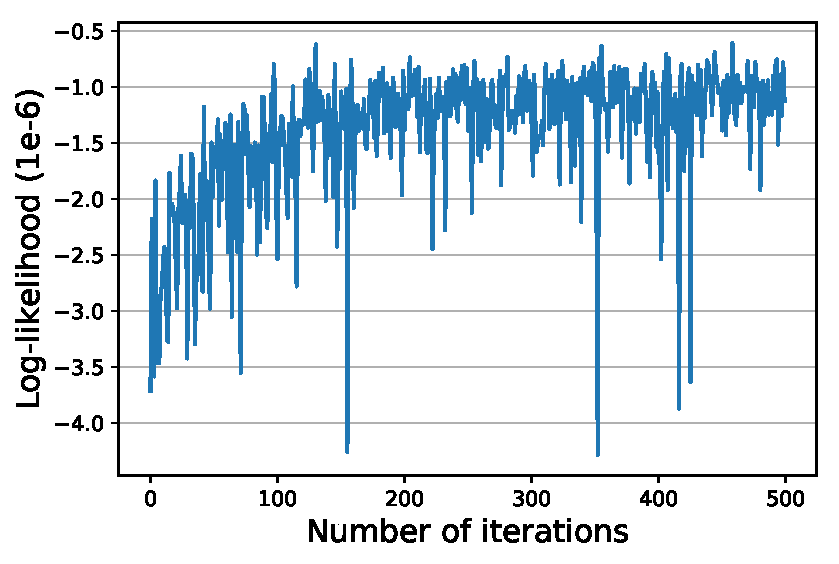
\includegraphics[width=3.5in]{ch5Fig4.pdf}
\caption{LL vs. training epochs.}
\label{ch5fig4}
\end{figure}

\section{Experiments}
\label{ch5sec5}
In this Section, we use our attentive state-space framework to model cystic fibrosis (CF) progression trajectories. CF is a life-shortening disease that causes lung dysfunction, and is the most common genetic disease in Caucasian populations \cite{szczesniak2017phenotypes}. Experimental details are listed hereunder.\\ 
\\
{\bf Implementation.}\,\,We implemented our model using \texttt{Tensorflow}. The LSTM cells in both the attention network (Figure \ref{ch5fig2}) and the inference network (Figure \ref{ch5fig3}) had 2 hidden layers of size 100. The model and inference networks were trained using ADAM with a learning rate of $5 \times 10^{-4}$, and a mini-batch size of 100. The same hyperparameters' setting was used for all baseline models involving RNNs. All results reported in this Section where obtained via 5-fold cross-validation.\\
\\
{\bf Data description.}\,\,We used data from a cohort of patients enrolled in the UK CF registry, a database held by the UK CF trust\footnote{\url{https://www.cysticfibrosis.org.uk/the-work-we-do/uk-cf-registry/}}. The dataset records annual follow-ups for 10,263 patients over the period from 2008 and 2015, with a total of 60,218 hospital visits. Each patient is associated with 90 variables, including information on 36 possible treatments, diagnoses for 31 possible comorbidities and 16 possible infections, in addition to biomarkers and demographic information. The FEV1 biomarker is the main measure of severity in CF patients \cite{sanders2010return}.\\
\\
{\bf Training.}\,\,In Figure \ref{ch5fig4}, we show the model's log-likelihood (LL) versus the number of training epochs. As we can see, the more training iterations we apply, the better the model likelihood gets: it jumped from $-4 \times 10^{-6}$ in the initial iterations to $-8 \times 10^{-5}$ after training was completed. The best value of the log-likelihood is 0, which is achieved when the inference network $q_{\phi}(z_t\,|\,\boldsymbol{\vec{x}}_T)$ coincides with the true model $p_{\theta}(z_t\,|\,\boldsymbol{\vec{x}}_T)$, and the observed data likelihood given the model is 1. Attentive inference is accurate because it utilizes the minimally sufficient set if past information, which reduces the variance in gradient estimates (Section \ref{ch5sec33}).\\
\\
{\bf Use cases.}\,\,We assess our model with respect to the two use cases it was designed for: (1) extracting clinical knowledge on disease progression mechanisms from the data, and (2) predicting a patient's health trajectory over time. We assess each use case in Sections \ref{ch5sec51} and \ref{ch5sec52}.  

\begin{figure}[h]
\centering
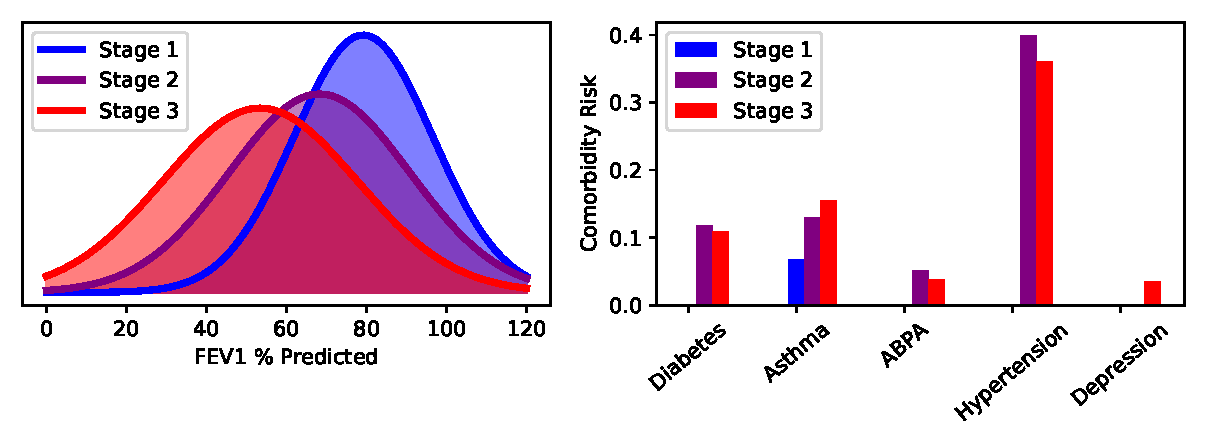
\includegraphics[width=5.5in]{ch5Fig5.pdf}
\caption{Distribution of observations in each progression stage.}
\label{ch5fig5}
\end{figure}

\subsection{Understanding CF Progression Mechanisms}
\label{ch5sec51}
{\bf Population-level phenotyping.}\,\,Our model learned a representation of $K=3$ CF progression stages (Stages 1, 2 and 3) in an unsupervised fashion, i.e., each stage is a realization of the hidden state $z_t$. As we show in what follows, each learned progression stage corresponded to a clinically distinguishable phenotype of disease activity. The learned baseline transition matrix was
\begin{align}
\boldsymbol{P} = \begin{bmatrix}
\, 0.85 & 0.10 & 0.05  \, \\
\, 0.13 & 0.72 & 0.15 \, \\
\, 0.24 & 0.10 & 0.66 \,
  \end{bmatrix}. \nonumber
%\label{eq00X2}
\end{align}   

The FEV1 biomarker is currently used by clinicians as a proximal measure of a patient's health in order to guide clinical and therapeutic decisions \cite{braun2011cystic}. In order to check that the learned progression stages correspond to different levels of disease severity, we plot the estimated mean of the emission distribution for the FEV1 biomarker in Stages 1, 2 and 3 in Figure \ref{ch5fig5} (left). As we can see from Figure \ref{ch5fig5} (left), the mean values of the FEV1 biomarker in each stage were $79\%$, $68\%$ and $53\%$, respectively. These values matched with the cutoff values on FEV1 used in current guidelines for referring critically-ill patients to a lung transplant \cite{braun2011cystic}. Thus, the learned progression stages can be translated into actionable information for clinical decision-making.

\begin{table*}[t]
\centering \scalebox{1}{\footnotesize
%\begin{tcolorbox}[tab3,tabularx={l||ccccc}] %
\begin{tabular}{l||ccccc}
 & {\footnotesize {\bf Diabetes}} & {\footnotesize {\bf ABPA}} & {\footnotesize {\bf Depression}} & {\footnotesize {\bf Pancreatitus}} & {\footnotesize {\bf P. Aeruginosa}}    \\
{\,\,\,\,\,\,\,\,\,\,\,\,\,\,\,\,\,\,\,\textbf{Model}} & {AUC-ROC} & AUC-ROC & AUC-ROC & AUC-ROC & AUC-ROC \\
\hline \hline
{\textbf{Attentive SS}} & {\bf \mbox{0.709 $\pm$ 0.02}} & {\bf \mbox{0.787 $\pm$ 0.01}} & {\bf \mbox{0.751 $\pm$ 0.03}} & \mbox{\bf 0.696 $\pm$ 0.04} & {\bf \mbox{0.680 $\pm$ 0.01}}  \\ 
{\textbf{HMM}} & \mbox{0.625 $\pm$ 0.02} & \mbox{0.686 $\pm$ 0.03} & \mbox{0.667 $\pm$ 0.08} & \mbox{0.625 $\pm$ 0.04} & \mbox{0.610 $\pm$ 0.02} \\  
{\textbf{RNN}} & \mbox{0.634 $\pm$ 0.03} & \mbox{0.727 $\pm$ 0.10} & \mbox{0.575 $\pm$ 0.01}  & \mbox{{0.590 $\pm$ 0.06}} & \mbox{0.654 $\pm$ 0.01}  \\   
{\textbf{LSTM}} & \mbox{0.675 $\pm$ 0.03} & \mbox{0.740 $\pm$ 0.07} & \mbox{0.609 $\pm$ 0.12} & \mbox{0.578 $\pm$ 0.05} & \mbox{0.671 $\pm$ 0.01} \\
{\textbf{RETAIN}} & \mbox{0.610 $\pm$ 0.06} & \mbox{0.718 $\pm$ 0.05} & \mbox{0.580 $\pm$ 0.09} & \mbox{0.600 $\pm$ 0.08} & \mbox{0.676 $\pm$ 0.02} \\    
\end{tabular}}
\caption{Performance of the different competing models for the 5 prognostic tasks.}
\label{ch5Table3}
\end{table*}

The progression stages learned by our model represented clinically distinguishable phenotypes with respect to multiple clinical variables. To illustrate these phenotypes, in Figure \ref{ch5fig5} (right) we plot the risks of various comorbities (Diabetes, asthma, ABPA, hypertension and depression) for patients in the 3 CF progression stages learned by the model. (Those risks were obtained directly from the learned emission distribution corresponding to the binary component $x^b_t$ of the clinical observation $x_t$.) As we can see, the incidences of those comorbidities and infections increase significantly in the more severe progression Stages 2 and 3 as compared to Stage 1.\\
\\
{\bf Individualized~contextual~diagnosis.} Population level modeling of disease stages can be already obtained with simple HMM models, but our model captures more complex dynamics that are specific to individuals, and can be made non-Markovian and non-stationary depending on the patient's context. To demonstrate the complex and non-stationary nature of the learned state dynamics, we plot the average attention weights assigned to the patients' previous state realizations in every "chronological" time step of a patient trajectory. The average attention weights per time step is plotted in Figure \ref{ch5fig6}.

\begin{figure}
\centering
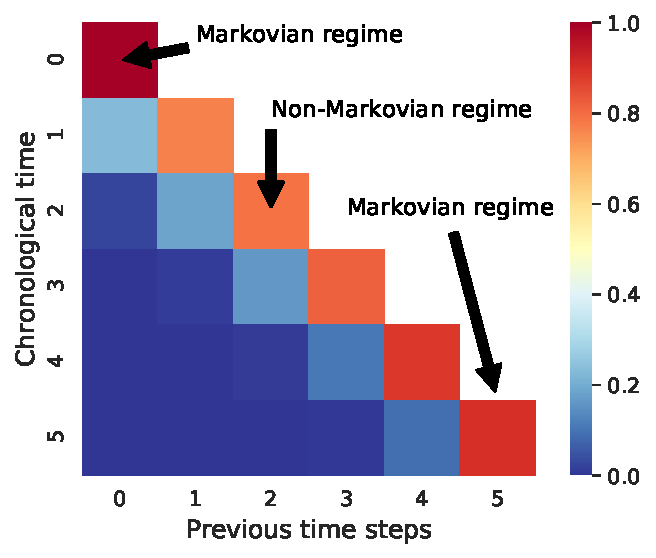
\includegraphics[width=4in]{ch5Fig6.pdf}
\caption{Average attention weights over time.}
\label{ch5fig6}
\end{figure}

As we can see, a patient's state trajectory behaves in a quasi-Markovian fashion (only current state takes all the weight) only on its edges. That is, at the first time step and the last time step, the only thing that matters for prediction is the patient's current state. This is because in the first time step, the patient has no history, whereas in the final step, the patient is already in the most severe state and hence her current health deterioration depends overrides all past clinical events. Memory becomes important only in intermediate Stages --- this is because patients in Stages 2 and 3 are more likely to have been diagnosed with more comorbidities in the past.

 
\subsection{Predicting Prognosis}
\label{ch5sec52}
As we have seen in Section \ref{ch5sec51}, our model is capable of extracting clinical intelligence from data, but does this compromise its predictive ability? To test the predictive ability of attentive state-space models, we sequentially predict the 1-year risk of 4 comorbidities (ABPA, diabetes, depression and pancreatitus), and 1 lung infections (Pseudomonas Aeruginosa) that are common in the CF population. We use the area under receiver operating characteristic curve (AUC-ROC) for performance evaluation. We report average AUC-ROC with 95$\%$ confidence intervals. We compare our model with 4 baselines: a vanilla RNN and an LSTM trained for sequence prediction, a state-of-the-art predictive model for healthcare data known as RETAIN \cite{kwon2019retainvis,choi2016retain}, and an HMM. 

As we can see in Table \ref{ch5Table3}, our model did not incur any performance loss when compared to models trained and tailored for the given prediction task (RNN, LSTM and RETAIN), and was in fact more accurate on all of the 5 tasks. The source of the predictive power in attentive state-space models comes from the usage of LSTM networks to model state dynamics in a low-dimensional space that summarizes the 90 variables associated with each patient. While HMMs can also learn interpretable representations of disease progression, they displayed modest predictive performance because of their oversimplified Markovian dynamics. Because attentive state-space models are capable of combining the interpretational benefits of probabilistic models and the predictive strength of deep learning, we envision them being used for large-scale disease phenotyping and clinical decision-making. 

\part{Application to Clinical Data}

\chapter{Predicting Deterioration of Lung Function in Cystic Fibrosis}
\section{Background}
\label{ch6sec0}
Cystic fibrosis (CF) is an autosomal recessive disease caused by the presence of mutations in both alleles at the cystic fibrosis transmembrane conductance regulator (CFTR) gene, and is the most common genetic disease in Caucasian populations\cite{adler2008genetic, fanen2014genetics}. Impaired CFTR functionality gives rise to different forms of lung dysfunction, all of which eventually lead to progressive respiratory failure\cite{mogayzel2014cystic, szczesniak2017phenotypes}. Despite recent therapeutic progress that significantly improved CF prognosis\cite{rowe2012progress}, only half of the current CF population are expected to live to over 40 years old \cite{mackenzie2014longevity}. Lung transplantation (LT) is recommended for patients with end-stage respiratory failure as a means to improved life expectancy \cite{flume1998cystic, liou2001survival, hofer2009true}. Unfortunately, there are more LT candidates than available lung donors \cite{flume1998cystic}, and in addition, the LT procedure is accompanied by serious risks of subsequent post-transplant complications\cite{mayer2002developing}. An effective LT referral policy should ensure an efficient allocation of the scarce donor lungs by precisely identifying high-risk patients as candidates for transplant, without overwhelming the LT waiting list with low-risk patients for whom a LT might be an unnecessary exposure to the risk of post-transplant complications\cite{liou2005use}.    

Current consensus guidelines, such as those recommended by the International Society for Heart and Lung Transplantation (ISHLT)\cite{weill2015consensus}, consider referring a patient for LT evaluation when the forced expiratory volume (FEV$_1$) drops below 30$\%$ of its predicted nominal value. This guideline, which is widely followed in clinical practice\cite{hook2012selecting,hirche2014practical}, is based mainly on the seminal study by Kerem {\it et. al}\cite{kerem1992prediction}, which identified FEV$_1$ as the main predictor of mortality in CF patients using survival data from a cohort of Canadian CF patients (patients eligible 1977-1989). While the FEV$_1$ biomarker has been repeatedly confirmed to be a strong predictor of mortality in CF patients\cite{milla1998risk,mayer2002developing,wojewodka2014candidate}, recent studies have shown that the survival behavior of CF patients with FEV$_1<$30$\%$ exhibits substantial heterogeneity\cite{heterogg}, and that the improvements in CF prognosis over the past years have changed the epidemiology and demography of CF populations\cite{urquhart2013deaths,stephenson2017changing}, which may have consequently altered the relevant CF risk factors (A striking example of a significant change in the demography of the CF population is the sharp decline in pediatric mortality in recent years\cite{urquhart2013deaths}.) However, none of the existing prognostic models that combine multiple risk factors\cite{hayllar1997prognostic,liou2001predictive,buzzetti2012validation,aaron2015statistical} have been able to demonstrate a significant improvement in mortality prediction compared to the FEV$_1$ criterion in terms of the positive predictive value, which is a proximal measure for the rate of premature LT referral (low-risk patients referred to a transplant)\cite{mayer2002developing}. 

The goal of this Chapter is to develop a CF prognostic model that can guide clinical decision-making by precisely selecting high-risk patients for LT referral. We use the automated ML algorithm developed in Chapter 4 (AutoPrognosis) to accomplish this goal. In particular, we apply AutoPrognosis to discover an accurate, data-driven prognostic model on the basis of a contemporary cohort from the UK CF registry; a database that includes 99$\%$ of the CF population in the UK\cite{CFReg,CFReg2,fink2017data}. 

\section{Data and Experimental Setup}
\label{ch6sec1}
Experiments were conducted using retrospective longitudinal data from the UK cystic fibrosis Registry; a database sponsored and hosted by the UK cystic fibrosis Trust \cite{CFReg}. The registry comprises a list of annual follow-up variables for individual CF patients that includes demographics, genetic mutations, airway colonization and microbiological infections, comorbidities and complications, transplantation, hospitalization, spirometry and therapeutic management. We used AutoPrognosis to automatically construct a prognostic model for predicting 3-year mortality (a realistic waiting time in a lung transplantation waiting list \cite{mayer2002developing}) based on the follow-up variables at baseline. 

\begin{sidewaystable}
\centering
{\footnotesize
\begin{tabular}{|l|lll|l|lll|}
\hline
\textcolor{black!60!black}{{\bf \footnotesize Variable}} & \textcolor{black!60!black}{{\bf \footnotesize Alive \& no LT}} & \textcolor{black!60!black}{{\bf \footnotesize Death/LT}} & \textcolor{black!60!black}{{\bf \footnotesize \textit{p}-value}} & \textcolor{black!60!black}{{\bf \footnotesize Variable}} & \textcolor{black!60!black}{{\bf \footnotesize Alive \& no LT}} & \textcolor{black!60!black}{{\bf \footnotesize Death/LT}} & \textcolor{black!60!black}{{\bf \footnotesize \textit{p}-value}} \\
\rule{0pt}{10pt} & \textcolor{black!75!black}{{\footnotesize \normalfont n = 3,682 (\%)}} & \textcolor{black!75!black}{{\footnotesize \normalfont n = 382 (\%)}} & & & \textcolor{black!75!black}{{\footnotesize \normalfont n = 3,682 (\%)}} & \textcolor{black!75!black}{{\footnotesize \normalfont n = 382 (\%)}} & \\
\hline
\hline
{\footnotesize \bf Gender (\footnotesize $\%$ male)} & {\footnotesize \normalfont 2,027 (55.0)} & {\footnotesize \normalfont 192 (50.2)} & {\footnotesize \normalfont 0.075} & {\footnotesize \it Pancreatic} &  &  & \rule{0pt}{2.6ex} \\
{\footnotesize \bf Age (years)$^{\mathsection}$} & {\normalfont \footnotesize 27.6 (12)} & {\normalfont \footnotesize 29.2 (14)} & {\normalfont \footnotesize $<$0.001} & \,\,\,{\footnotesize \normalfont Cirrhosis} & {\footnotesize \normalfont 86 (2.3)} & {\footnotesize \normalfont 24 (6.3)} & {\footnotesize \normalfont $<$0.001} \\
{\footnotesize \bf Height (cm)$^{\mathsection}$} & {\normalfont \footnotesize 168.0 (14)} & {\normalfont \footnotesize 166.0 (15)} & {\normalfont \footnotesize $<$0.001} & \,\,\,{\footnotesize \normalfont Liver Disease} & {\footnotesize \normalfont 578 (15.7)} & {\footnotesize \normalfont 81 (21.2)} & {\footnotesize \normalfont 0.007} \\ 
{\footnotesize \bf Weight (kg)$^{\mathsection}$} & {\normalfont \footnotesize 63.1 (17)} & {\normalfont \footnotesize 54.8 (15)} & {\normalfont \footnotesize $<$0.001} & \,\,\,{\footnotesize \normalfont Pancreatitis} & {\footnotesize \normalfont 57 (1.5)} & {\footnotesize \normalfont 3 (0.8)} & {\footnotesize \normalfont 0.368} \\ 
{\footnotesize \bf BMI (kg/m$^2$)$^{\mathsection}$} & {\normalfont \footnotesize 22.3 (4)} & {\normalfont \footnotesize 20.1 (4)} & {\normalfont \footnotesize $<$0.001} &\,\,\,{\footnotesize \normalfont Liver Enzymes} & {\footnotesize \normalfont 521 (14.1)} & {\footnotesize \normalfont 98 (25.7)} & {\footnotesize \normalfont $<$0.001} \\
{\footnotesize \bf CFTR genotype} &  &  &  &\,\,\,{\footnotesize \normalfont Gall Bladder} & {\footnotesize \normalfont 20 (0.5)} & {\footnotesize \normalfont 3 (0.8)} & {\footnotesize \normalfont 0.472} \\
\,\,\,{\footnotesize \normalfont Homozygous} & {\normalfont \footnotesize 1,784 (48.4)} & {\normalfont \footnotesize 208 (54.4)} & {\normalfont \footnotesize $<$0.001} &\,\,\,{\footnotesize \normalfont GI Bleed (variceal)} & {\footnotesize \normalfont 3 (0.1)} & {\footnotesize \normalfont 3 (0.8)} & {\footnotesize \normalfont 0.013} \\
\,\,\,{\footnotesize \normalfont Heterozygous} & {\normalfont \footnotesize 1,240 (33.7)} & {\normalfont \footnotesize 92 (24.0)} & {\normalfont \footnotesize $<$0.001} & {\footnotesize \it Gastrointestinal} &  &  &  \\
\,\,\,{\footnotesize \normalfont $\Delta$F508} & {\normalfont \footnotesize 3,189 (86.6)} & {\normalfont \footnotesize 325 (85.0)} & {\normalfont \footnotesize 0.388} &\,\,\,{\footnotesize \normalfont GERD} & {\footnotesize \normalfont 747 (20.3)} & {\footnotesize \normalfont 100 (26.2)} & {\footnotesize \normalfont 0.008} \\
\,\,\,{\footnotesize \normalfont G551D} & {\normalfont \footnotesize 224 (6.0)} & {\normalfont \footnotesize 15 (3.9)} & {\normalfont \footnotesize 0.108} &\,\,\,{\footnotesize \normalfont GI Bleed (no variceal)} & {\footnotesize \normalfont 4 (0.1)} & {\footnotesize \normalfont 1 (0.3)} & {\footnotesize \normalfont 0.390} \\ 
\,\,\,{\footnotesize \normalfont Class I} & {\normalfont \footnotesize 169 (4.6)} & {\normalfont \footnotesize 23 (6.0)} & {\normalfont \footnotesize 0.205}
 &\,\,\,{\footnotesize \normalfont Intestinal Obstruction} & {\footnotesize \normalfont 303 (8.2)} & {\footnotesize \normalfont 33 (8.6)} & {\footnotesize \normalfont 0.770} \\
\,\,\,{\footnotesize \normalfont Class II} & {\normalfont \footnotesize 3,207 (87.1)} & {\normalfont \footnotesize 326 (85.3)} & {\normalfont \footnotesize 0.338} & {\footnotesize \it Musculoskeletal} &  &  &  \\ 
\,\,\,{\footnotesize \normalfont Class III} & {\normalfont \footnotesize 3,281 (89.1)} & {\normalfont \footnotesize 330 (86.3)} & {\normalfont \footnotesize 0.123} &\,\,\,{\footnotesize \normalfont Arthropathy} &  {\footnotesize \normalfont 338 (9.2)} & {\footnotesize \normalfont 52 (13.6)} & {\footnotesize \normalfont 0.008} \\
\,\,\,{\footnotesize \normalfont Class IV} & {\normalfont \footnotesize 184 (5.0)} & {\normalfont \footnotesize 4 (1.0)} & {\normalfont \footnotesize $<$0.001} &\,\,\,{\footnotesize \normalfont Bone Fracture} & {\footnotesize \normalfont 39 (1.1)} & {\footnotesize \normalfont 6 (1.6)} & {\footnotesize \normalfont 0.310}\\
\,\,\,{\footnotesize \normalfont Class V} & {\normalfont \footnotesize 130 (3.5)} & {\normalfont \footnotesize 8 (2.0)} & {\normalfont \footnotesize 0.179} &\,\,\,{\footnotesize \normalfont Osteopenia} & {\footnotesize \normalfont 710 (19.3)} & {\footnotesize \normalfont 126 (33.0)} & {\footnotesize \normalfont $<$0.001}\\
\,\,\,{\footnotesize \normalfont Class VI} & {\normalfont \footnotesize 3,189 (86.6)} & {\normalfont \footnotesize 325 (85.0)} & {\normalfont \footnotesize 0.388} & {\footnotesize \it Other} &  &  &  \\ 
\hline 
\end{tabular}}
\caption{Baseline characteristics of patients in the UK CF Registry on December 31\textsuperscript{st} 2012. ($^{\mathsection}$Continuous variables: median (inter-quartile range).)}
\label{ch6Table1}
\end{sidewaystable}

\begin{sidewaystable}
\centering
{\footnotesize
\begin{tabular}{|l|lll|l|lll|}
\hline
\textcolor{black!60!black}{{\bf \footnotesize Variable}} & \textcolor{black!60!black}{{\bf \footnotesize Alive \& no LT}} & \textcolor{black!60!black}{{\bf \footnotesize Death/LT}} & \textcolor{black!60!black}{{\bf \footnotesize \textit{p}-value}} & \textcolor{black!60!black}{{\bf \footnotesize Variable}} & \textcolor{black!60!black}{{\bf \footnotesize Alive \& no LT}} & \textcolor{black!60!black}{{\bf \footnotesize Death/LT}} & \textcolor{black!60!black}{{\bf \footnotesize \textit{p}-value}} \\
\rule{0pt}{10pt} & \textcolor{black!75!black}{{\footnotesize \normalfont n = 3,682 (\%)}} & \textcolor{black!75!black}{{\footnotesize \normalfont n = 382 (\%)}} & & & \textcolor{black!75!black}{{\footnotesize \normalfont n = 3,682 (\%)}} & \textcolor{black!75!black}{{\footnotesize \normalfont n = 382 (\%)}} & \\
\hline
\hline
{\footnotesize \bf Spirometry}$^{\mathsection}$ &  &  &  &\,\,\,{\footnotesize \normalfont Cancer} & {\footnotesize \normalfont 8 (0.2)} & {\footnotesize \normalfont 5 (1.3)} & {\footnotesize \normalfont 0.005} \\
\,\,\,{\footnotesize \normalfont FEV$_1$ (L)} & {\normalfont \footnotesize 2.34 (1.4)} & {\normalfont \footnotesize 0.99 (0.6)} & {\normalfont \footnotesize $<$0.001} &\,\,\,{\footnotesize \normalfont Diabetes} & {\footnotesize \normalfont 906 (24.6)} & {\footnotesize \normalfont 199 (52.1)} & {\footnotesize \normalfont $<$0.001} \\
\,\,\,{\footnotesize \normalfont FEV$_1 \%$} & {\normalfont \footnotesize 67.8 (35)} & {\normalfont \footnotesize 29.6 (19)} & {\normalfont \footnotesize $<$0.001} &\,\,\,{\footnotesize \normalfont CFRD} & {\footnotesize \normalfont 1,096 (29.8)} & {\footnotesize \normalfont 223 (58.4)} & {\footnotesize \normalfont $<$0.001} \\
{\footnotesize \bf Lung Infections} &  &  &  &\,\,\,{\footnotesize \normalfont Hypertension} & {\footnotesize \normalfont 121 (3.3)} & {\footnotesize \normalfont 23 (6.0)} & {\footnotesize \normalfont 0.012} \\
\,\,\,{\footnotesize \normalfont B. Cepacia} & {\footnotesize \normalfont 176 (4.8)} & {\footnotesize \normalfont 35 (9.2)} & {\footnotesize \normalfont 0.001} &\,\,\,{\footnotesize \normalfont Atypical Mycobacteria} & {\footnotesize \normalfont 127 (3.4)} & {\footnotesize \normalfont 17 (4.5)} & {\footnotesize \normalfont 0.308} \\
\,\,\,{\footnotesize \normalfont P. Aeruginosa} & {\footnotesize \normalfont 2,190 (59.5)} & {\footnotesize \normalfont 295 (77.2)} & {\footnotesize \normalfont $<$0.001} &\,\,\,{\footnotesize \normalfont Hearing Loss} & {\footnotesize \normalfont 82 (2.2)} & {\footnotesize \normalfont 26 (6.8)} & {\footnotesize \normalfont $<$0.001} \\
\,\,\,{\footnotesize \normalfont MRSA} & {\footnotesize \normalfont 154 (4.2)} & {\footnotesize \normalfont 17 (4.5)} & {\footnotesize \normalfont 0.789} &\,\,\,{\footnotesize \normalfont Depression} & {\footnotesize \normalfont 257 (7.0)} & {\footnotesize \normalfont 59 (15.4)} & {\footnotesize \normalfont $<$0.001} \\
\,\,\,{\footnotesize \normalfont Aspergillus} & {\footnotesize \normalfont 478 (13.0)} & {\footnotesize \normalfont 70 (18.3)} & {\footnotesize \normalfont 0.006} &{\footnotesize \bf Inhaled Antibiotics} & {\footnotesize \normalfont 2,194 (59.6)} & {\footnotesize \normalfont 280 (73.3)} & {\footnotesize \normalfont $<$0.001} \\
\,\,\,{\footnotesize \normalfont NTM} & {\footnotesize \normalfont 186 (5.1)} & {\footnotesize \normalfont 20 (5.2)} & {\footnotesize \normalfont 0.902} &{\footnotesize \bf Muco-active Therapies} &  &  &  \\ 
\,\,\,{\footnotesize \normalfont H. Influenza} & {\footnotesize \normalfont 191 (5.2)} & {\footnotesize \normalfont 10 (2.6)} & {\footnotesize \normalfont 0.025} &\,\,\,{\footnotesize \normalfont DNase} & {\footnotesize \normalfont 2,057 (55.9)} & {\footnotesize \normalfont 297 (77.7)} & {\footnotesize \normalfont $<$0.001} \\
\,\,\,{\footnotesize \normalfont E. Coli} & {\footnotesize \normalfont 17 (0.5)} & {\footnotesize \normalfont 2 (0.5)} & {\footnotesize \normalfont 0.698} &\,\,\,{\footnotesize \normalfont Hypertonic Saline} & {\footnotesize \normalfont 859 (23.3)} & {\footnotesize \normalfont 109 (28.5)} & {\footnotesize \normalfont 0.027} \\
\,\,\,{\footnotesize \normalfont K. Pneumoniae} & {\footnotesize \normalfont 10 (0.3)} & {\footnotesize \normalfont 3 (0.8)} & {\footnotesize \normalfont 0.116} & {\footnotesize \bf Promixin} & {\footnotesize \normalfont 765 (20.8)} & {\footnotesize \normalfont 71 (18.6)} & {\footnotesize \normalfont 0.352} \\
\,\,\,{\footnotesize \normalfont Gram-negative} & {\footnotesize \normalfont 14 (0.4)} & {\footnotesize \normalfont 4 (1.0)} & {\footnotesize \normalfont 0.082} & {\footnotesize \bf Tobramycin} & {\footnotesize \normalfont 110 (3.0)} & {\footnotesize \normalfont 28 (7.3)} & {\footnotesize \normalfont $<$0.001} \\
\,\,\,{\footnotesize \normalfont ALCA} & {\footnotesize \normalfont 97 (2.6)} & {\footnotesize \normalfont 25 (6.5)} & {\footnotesize \normalfont $<$0.001} & {\footnotesize \bf iBuprofen} & {\footnotesize \normalfont 8 (0.2)} & {\footnotesize \normalfont 2 (0.5)} & {\footnotesize \normalfont 0.241} \\
\,\,\,{\footnotesize \normalfont Staph. Aureus} & {\footnotesize \normalfont 1,175 (31.9)} & {\footnotesize \normalfont 64 (16.8)} & {\footnotesize \normalfont $<$0.001} & {\footnotesize \bf Oral Corticosteroids} & {\footnotesize \normalfont 347 (9.4)} & {\footnotesize \normalfont 122 (31.9)} & {\footnotesize \normalfont $<$0.001} \\ 
{\footnotesize \bf Comorbidities} &  &  &  & {\footnotesize \bf Non-IV Hospitalization} & {\footnotesize \normalfont 312 (8.5)} & {\footnotesize \normalfont 62 (16.2)} & {\footnotesize \normalfont $<$0.001} \\
{\footnotesize \it Respiratory} &  &  &  & {\footnotesize \bf Non-invasive Ventilation} & {\footnotesize \normalfont 161 (4.4)} & {\footnotesize \normalfont 82 (21.5)} & {\footnotesize \normalfont $<$0.001} \\
\,\,\,{\footnotesize \normalfont ABPA} & {\footnotesize \normalfont 432 (11.7)} & {\footnotesize \normalfont 71 (18.6)} & {\footnotesize \normalfont $<$0.001} & {\footnotesize \bf Oxygen Therapy} & {\footnotesize \normalfont 279 (7.6)} & {\footnotesize \normalfont 205 (53.7)} & {\footnotesize \normalfont $<$0.001}\\
\,\,\,{\footnotesize \normalfont Nasal Polyps} & {\footnotesize \normalfont 123 (3.3)} & {\footnotesize \normalfont 4 (1.0)} & {\footnotesize \normalfont 0.012} &\,\,\,{\footnotesize \normalfont Continuous} & {\footnotesize \normalfont 13 (0.4)} & {\footnotesize \normalfont 75 (19.6)} & {\footnotesize \normalfont $<$0.001}\\
\,\,\,{\footnotesize \normalfont Asthma} & {\footnotesize \normalfont 578 (15.7)} & {\footnotesize \normalfont 58 (15.2)} & {\footnotesize \normalfont 0.825} &\,\,\,{\footnotesize \normalfont Nocturnal} & {\footnotesize \normalfont 42 (1.1)} & {\footnotesize \normalfont 48 (12.6)} & {\footnotesize \normalfont $<$0.001}\\
\,\,\,{\footnotesize \normalfont Sinus Disease} & {\footnotesize \normalfont 486 (13.2)} & {\footnotesize \normalfont 41 (10.7)} & {\footnotesize \normalfont 0.200} &\,\,\,{\footnotesize \normalfont Exacerbation} & {\footnotesize \normalfont 100 (2.7)} & {\footnotesize \normalfont 46 (12.0)} & {\footnotesize \normalfont $<$0.001} \\
\,\,\,{\footnotesize \normalfont Hemoptysis} & {\footnotesize \normalfont 48 (1.3)} & {\footnotesize \normalfont 11 (2.9)} & {\footnotesize \normalfont 0.022} &\,\,\,{\footnotesize \normalfont Pro re nata} & {\footnotesize \normalfont 37 (1.0)} & {\footnotesize \normalfont 29 (7.6)} & {\footnotesize \normalfont $<$0.001} \\
\hline 
\end{tabular}}
\caption{Baseline characteristics of patients in the UK CF Registry on December 31\textsuperscript{st} 2012. ($^{\mathsection}$Continuous variables: median (inter-quartile range).)}
\label{ch6Table2}
\end{sidewaystable}

All experiments were conducted using data for a baseline cohort comprising patients' follow-up variables collected in 2012: this was the most recent cohort for which 3-year mortality data was available. A total of 115 variables were associated with every patient, all of which were fed into AutoPrognosis in order to encourage an agnostic, data-driven approach for discovering risk factors. Since transplantation decisions are mostly relevant for adults (93.75$\%$ of transplantation operations recorded in the registry were performed in adults), we excluded pediatric patients, and included only patients who were more than 18 years old. (Deaths in children with CF are now very rare in developed countries \cite{urquhart2013deaths, nkam20173}.) Outcomes are defined as death or lung transplantation within 3 years of the baseline data collection date. Patients who were lost to follow-up or have already undergone a transplant before 2012 were excluded. Figure \ref{ch6fig1} depicts a flow chart of the data assembly process involved in our analysis. Of the 4,532 patients who were aged 18 years or older in 2012, a total of  114 patients underwent a lung transplant before their 2012 annual review, and a total of 354 patients were lost to follow-up. Of the remaining 4,064 patients, 382 patients (9.4$\%$) experienced an adverse outcome within a 3-year period. 

\begin{figure}[t]
\centering
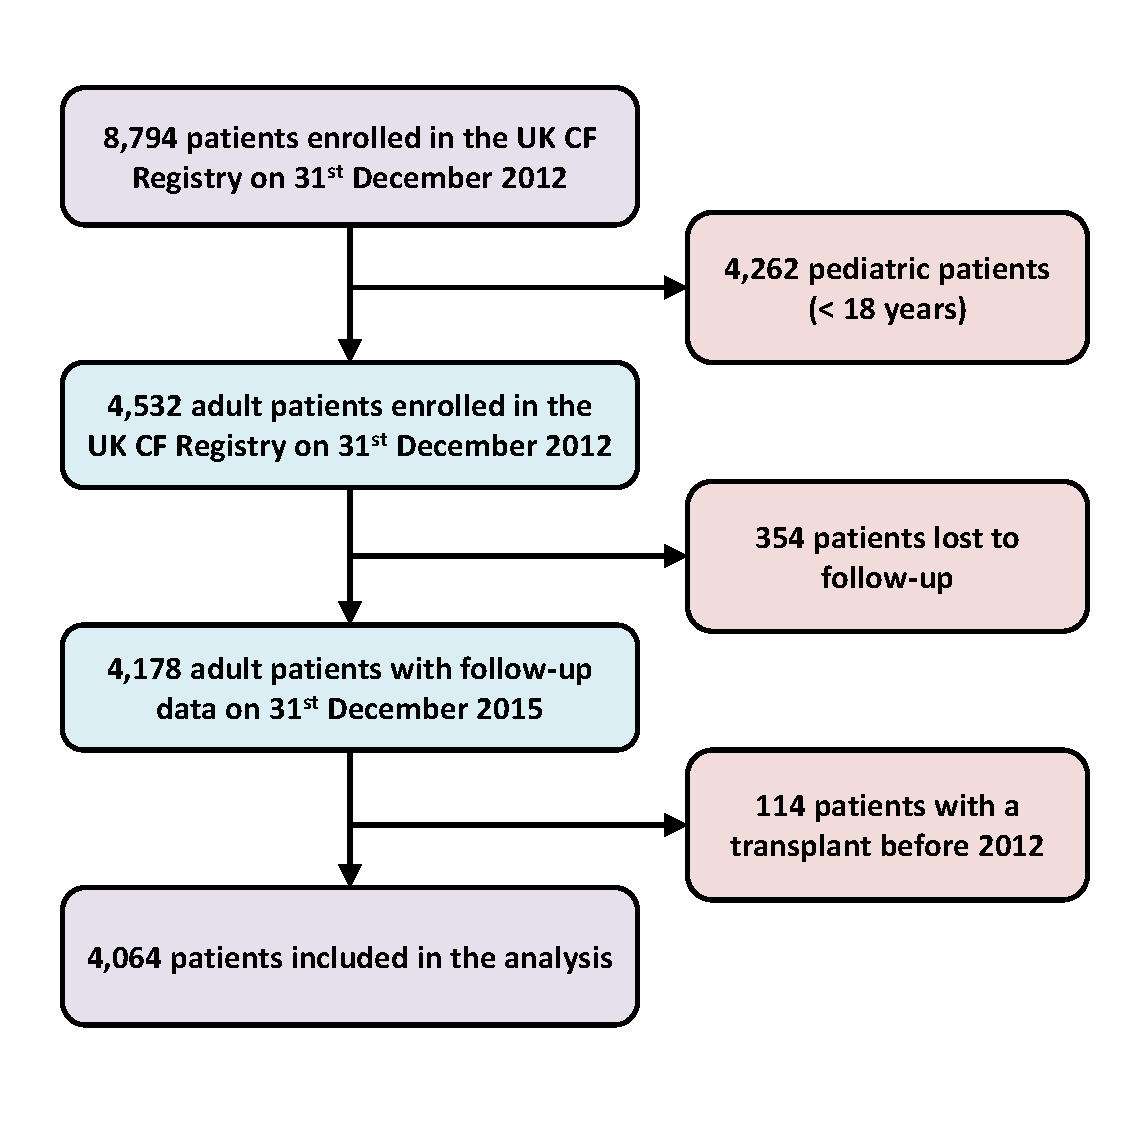
\includegraphics[width=4.25in]{ch6Fig1.pdf}
\caption{Patient selection and data assembly process.}
\label{ch6fig1}
\end{figure}

Of the 382 patients who experienced an adverse outcome, 266 died without receiving a transplant, 104 underwent a successful transplant, and 12 patients received a transplant but died within the 3-year horizon. The characteristics of the patients in the baseline cohort are provided in Tables \ref{ch6Table1} and \ref{ch6Table2}. The study population was stratified into two subgroups based on the endpoint outcomes and the characteristics of the two subgroups were compared using Fisher's exact test for discrete (and categorical) variables, and Mann-Whitney $U$ test for continuous variables. 

The number of CFTR mutations (in either alleles) whose frequencies in the cohort exceeded 1$\%$ was 66, with the most frequent five mutations being $\Delta$F508, G551D, R117H, G542X, and 621+1G$\rightarrow$T. Previous studies on CF genetics have classified CFTR mutations into 6 different categories according to the mechanism by which they obstruct the synthesis and traffic of CFTR \cite{fanen2014genetics}. We used the CFTR genetic classification in order to cluster the (high-dimensional) genotype information. In particular, we converted the  genotype information of every patient into a vector of 9 binary features which encodes the following information: whether the CFTR mutation is homozygous, whether any of the two alleles carries a $\Delta$F508 or a G551D mutation, and the class to which the mutation carried by the patient belongs. 

\begin{figure}[t]
\centering
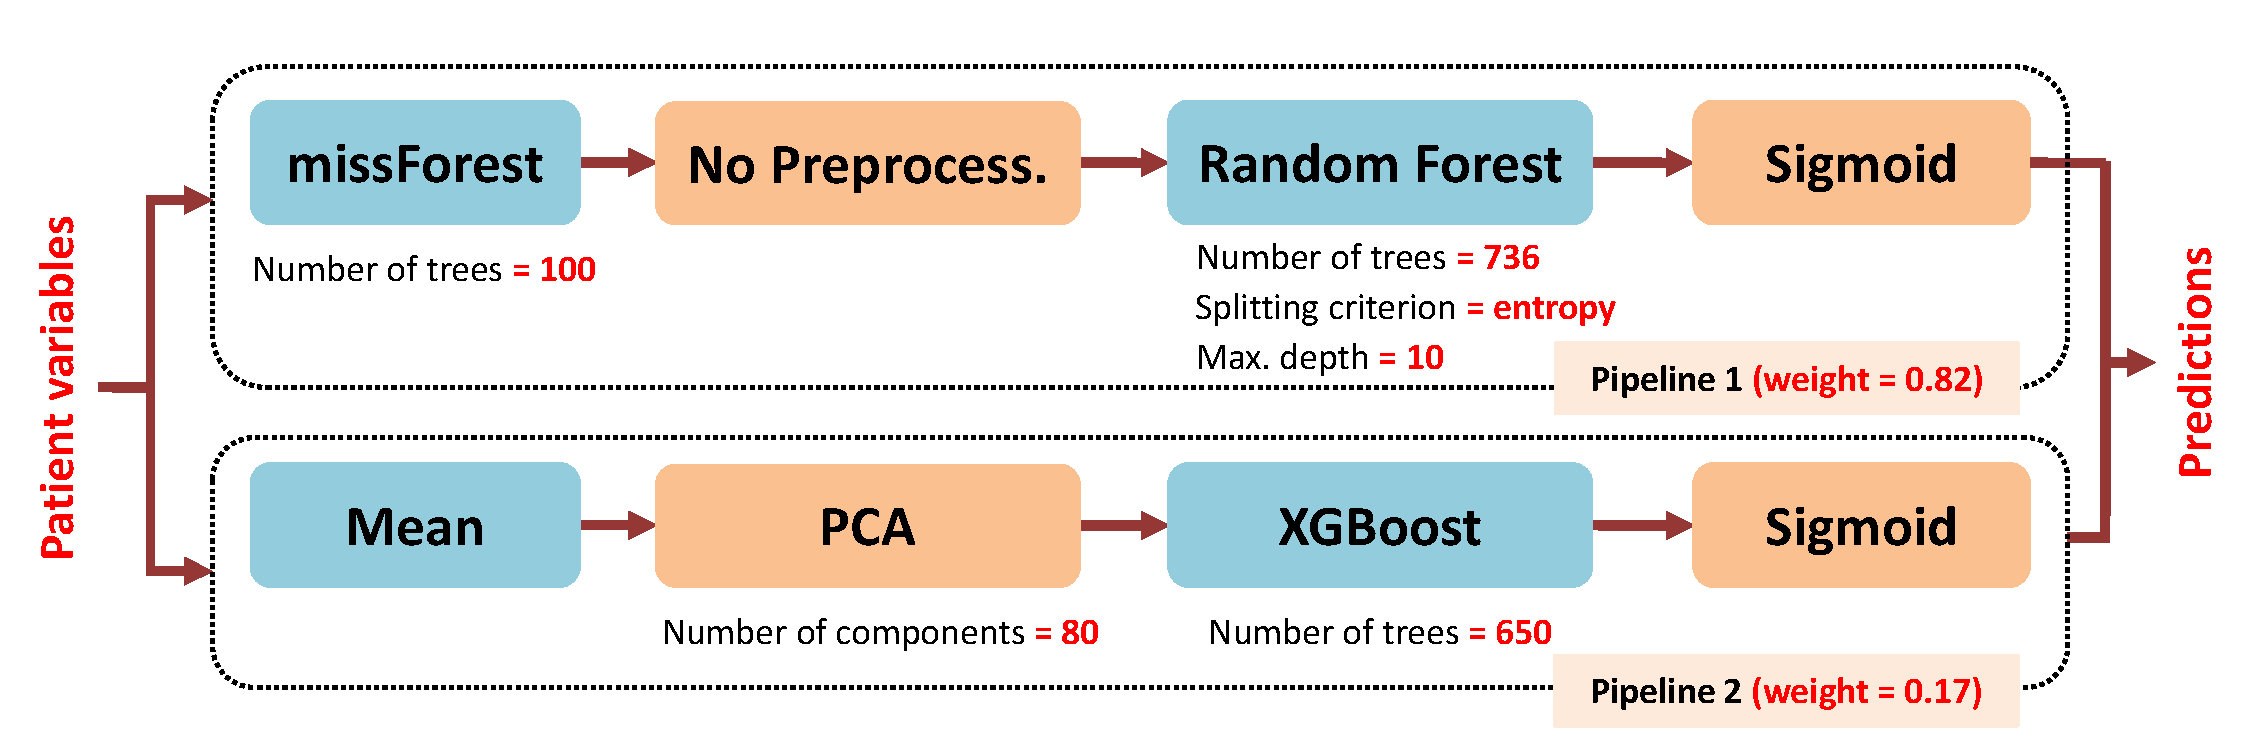
\includegraphics[width=5.5in]{ch6Fig2.pdf}
\caption{Schematic depiction for the in-sample model ft obtained by AutoPrognosis.}
\label{ch6fig2}
\end{figure}

\section{Training and Validation of AutoPrognosis}
\label{ch6sec2} 
All evaluations of diagnostic accuracy were obtained via 10-fold stratified cross-validation in order to assess the generalization performance, where a held-out sample was used to evaluate the performance of the model learned by AutoPrognosis in every fold using a mutually exclusive training sample. In every cross-validation fold, AutoPrognosis conducts up to 200 iterations of the Bayesian optimization procedure presented in Chapter 4, where in every iteration it explores a new pipeline and tunes its hyper-parameters. AutoPrognosis builds an ensemble of all the pipelines that it explored in which every pipeline is given a weight that is proportional to its empirical performance. The in-sample model fit obtained by AutoPrognosis is depicted in Figure \ref{ch6fig2}. The model combines two pipelines: the first uses {\it missForest} imputation\cite{stekhoven2011missforest} and a {\it random forest} classifier (with 736 trees) with no feature processing, whereas the second pipeline uses simple mean imputation, a PCA transformation with 80 components followed by an XGBoost classifier with 650 trees. Both pipelines used sigmoid regression for calibration. The in-sample area under receiver operating characteristic curve was 0.9714, and the model was well-calibrated, with a Brier score of 0.0543. 

\section{Results}
\label{ch6sec3}
\subsection{Systematic Review of Existing Risk Scores} 

We compared the diagnostic accuracy of AutoPrognosis with state-of-the-art prognostic models that were developed for predicting short-term CF outcomes. In order to identify and select the competing prognostic models, we searched PubMed for studies published in the last 10 years (in all languages) with the terms ``(cystic fibrosis) and survival and (prognostic or predictive model)". We filtered the relevant studies by their clinical end-points, focusing only on studies that defined the composite end-point of death and lung transplantation in a time horizon of less than 5 years. We identified 3 contemporary studies that developed and validated prognostic models using multicenter or registry data \cite{nkam20173,mccarthy2013cf,dimitrov2015cf,buzzetti2012validation}. In the first study, Buzzetti {\it et al.} \cite{buzzetti2012validation} developed a parsimonious multivariate logistic regression model for predicting 5-year outcomes for CF patients using 4 variables, and demonstrated that it outperforms the model developed by Liou {\it et al.} \cite{liou2001predictive} using retrospective data from 9 Italian CF centers. McCarthy {\it et al.} \cite{mccarthy2013cf} developed a predictive model, dubbed ``CF-ABLE", for predicting 4-year CF outcomes using 4 variables, and validated their model using data for 370 patients enrolled in the Irish CF registry data. Dimitrov {\it et al.} \cite{dimitrov2015cf} proposed a modified version of the CF-ABLE score, dubbed ``CF-ABLE-UK", which they (externally) validated through the UK CF registry data, reporting a c-statistic of 0.80 (95$\%$ CI: 0.79$-$0.83). More recently, Nkam {\it et al.} \cite{nkam20173} developed a multivariate logistic regression model for predicting 3-year CF outcomes using 8 risk factors. The model was internally validated through the French CF registry, reporting a c-statistic of 0.91 (95$\%$ CI: 0.89$-$0.92). We compared the diagnostic accuracy of AutoPrognosis with these 3 models as they considered similar clinical end-points and were validated on contemporary retrospective cohorts. 

All of the studies mentioned above explored the usage of only a few risk factors in model development. To the best of our knowledge, ours is the first study to investigate an agnostic, machine learning-based approach for discovering risk factors for CF using a representative cohort that covers the entire CF population in the UK. In order to assess the clinical utility of AutoPrognosis, we also compared its diagnostic accuracy with the simple FEV$_1$-based prediction rule proposed by Kerem {\it et al.} \cite{kerem1992prediction}, where a LT referral criterion that selects CF patients with an FEV$_1\%$ of less than 30$\%$ predicted was recommended. This simple prediction rule continues to be the main criterion for LT referral in current clinical practice guidelines \cite{hirche2014practical,hook2012selecting,orens2006international}. 

\subsection{Diagnostic Accuracy Evaluation} 

The main objective of CF prognostic models is to inform LT referral decisions \cite{mayer2002developing,flume1998cystic,braun2015impact,hirche2014practical}. Since donor lungs are scarce\cite{flume1998cystic,liou2005use,liou2001survival}, the clinical utility of a prognostic model should be quantified in terms of the model's ability to (precisely) identify patients who are truly at risk and hence should be allocated in a LT waiting list. Many of the previously developed models have been validated only through goodness-of-fit measures\cite{hayllar1997prognostic,aaron2015statistical}, which reveal little information about the models' actual clinical utility. The area under receiver operating characteristic (AUC-ROC) curve has been used to quantify the discriminative power of the models developed by Nkam {\it et al.} \cite{nkam20173}, McCarthy {\it et al.} \cite{mccarthy2013cf} and Buzzetti {\it et al.} \cite{buzzetti2012validation}. AUC-ROC is nevertheless a misleading quantifier for the usefulness of a CF prognostic model as it is insensitive to the prevalence of poor outcomes in the population, and assumes that positive and negative predictions are equally important \cite{swets1988measuring}. Since most patients would not need a LT at the 3-year horizon (the prevalence of poor outcomes is as low as 9.4$\%$), a model's AUC-ROC evaluation can be deceptively high, only reflecting a large number of ``easy" and ``non-actionable" true negative predictions, without reflecting the actual precision of the LT referral decisions guided by the model. The inappropriateness of AUC-ROC as a sole measure of diagnostic accuracy in the context of LT referral for CF patients was highlighted by Mayer-Hamblett {\it et al.} \cite{mayer2002developing}, where it was shown that models with seemingly high AUC-ROC can still have modest predictive values (refer to Table 3 therein). A detailed technical analysis of the shortcomings of the AUC-ROC in imbalanced datasets was recently conducted by Saito {\it et al.}\cite{saito2015precision}. 

In order to ensure a comprehensive assessment for the clinical usefulness of AutoPrognosis, we evaluated the {\it positive predictive values} (PPV) and {\it negative predictive values} (NPV) for all predictive models under consideration, in addition to the standard AUC-ROC metrics. (PPV is also known as the {\it precision} metric.) The PPV reflects the fraction of patients who are truly at risk among those identified by the model as high risk patients. A model's PPV characteristic best represents its clinical usefulness as it reflects the precision in the associated LT referral decisions\cite{mayer2002developing}. That is, at a fixed sensitivity, models with higher PPV would lead to fewer patients who are not at risk being enrolled in a transplant waiting list, resulting in a more effective lung allocation scheme with fewer premature referrals. 

\begin{sidewaystable}
\centering
\begin{tabular}{|c||c|c|c|c|c|}
\hline
{\bf Prognostic model} & {\bf AUC-ROC} & {\bf Youden's J statistic} & {\bf AUC-PR} & {\bf Average Precision} & {\bf $F_1$ score}      \\\hline\hline
{\footnotesize AutoPrognosis} & {\footnotesize 0.89 $\pm$ 0.01} & {\footnotesize 0.67 $\pm$ 0.02} & {\footnotesize 0.58 $\pm$ 0.04} & {\footnotesize 0.59 $\pm$ 0.04} & {\footnotesize 0.60 $\pm$ 0.03} \\\hline\hline\hline
{\footnotesize Nkam {\it et al.}\cite{nkam20173}, 2017} & {\footnotesize 0.86 $\pm$ 0.01} & {\footnotesize 0.58 $\pm$ 0.03} & {\footnotesize 0.50 $\pm$ 0.03} & {\footnotesize 0.48 $\pm$ 0.03} & {\footnotesize 0.52 $\pm$ 0.02} \\\hline
{\footnotesize Buzzetti {\it et al.}\cite{buzzetti2012validation}, 2012} & {\footnotesize 0.83 $\pm$ 0.01} & {\footnotesize 0.54 $\pm$ 0.03} & {\footnotesize 0.42 $\pm$ 0.02} & {\footnotesize 0.44 $\pm$ 0.03} & {\footnotesize 0.49 $\pm$ 0.02}  \\\hline
{\footnotesize CF-ABLE-UK \cite{dimitrov2015cf} (2015)} & {\footnotesize 0.77 $\pm$ 0.01} & {\footnotesize 0.48 $\pm$ 0.05} & {\footnotesize 0.28 $\pm$ 0.04} & {\footnotesize 0.20 $\pm$ 0.02} & {\footnotesize 0.34 $\pm$ 0.02} \\\hline
{\footnotesize FEV$_1\%$ predicted criterion\cite{kerem1992prediction}} & {\footnotesize 0.70 $\pm$ 0.01} & {\footnotesize 0.41 $\pm$ 0.02} & {\footnotesize 0.50 $\pm$ 0.02} & {\footnotesize 0.27 $\pm$ 0.02} & {\footnotesize 0.47 $\pm$ 0.01}  \\\hline\hline\hline
{\footnotesize SVM} & {\footnotesize 0.84 $\pm$ 0.03} & {\footnotesize 0.60 $\pm$ 0.05} & {\footnotesize 0.50 $\pm$ 0.09} & {\footnotesize 0.51 $\pm$ 0.09} & {\footnotesize 0.52 $\pm$ 0.07} \\\hline 
{\footnotesize Gradient Boosting} & {\footnotesize 0.87 $\pm$ 0.02} & {\footnotesize 0.63 $\pm$ 0.01} & {\footnotesize 0.55 $\pm$ 0.03} & {\footnotesize 0.55 $\pm$ 0.04} & {\footnotesize 0.56 $\pm$ 0.01} \\\hline
{\footnotesize Bagging} & {\footnotesize 0.83 $\pm$ 0.03} & {\footnotesize 0.58 $\pm$ 0.05} & {\footnotesize 0.51 $\pm$ 0.04} & {\footnotesize 0.47 $\pm$ 0.04} & {\footnotesize 0.52 $\pm$ 0.03}\\\hline\hline\hline
{\footnotesize TPOT} & {\footnotesize 0.84 $\pm$ 0.01} & {\footnotesize 0.56 $\pm$ 0.03} & {\footnotesize 0.51 $\pm$ 0.02} & {\footnotesize 0.49 $\pm$ 0.02} & {\footnotesize 0.51 $\pm$ 0.02} \\
\hline
\end{tabular}
\caption{Comparison of various diagnostic accuracy metrics (with 95$\%$ CI) for the prognostic models under consideration.}
\label{ch6Table3}
\end{sidewaystable} 

In Table \ref{ch6Table3}, we compare the performance of AutoPrognosis with the competing models in terms of various diagnostic accuracy metrics that capture the models' sensitivity, specificity and predictive values. In particular, we evaluate the models' AUC-ROC, Youden's J statistic, area under precision-recall curve (AUC-PR), average precision and the $F_1$ score. The AUC-ROC and Youden's J statistic characterize the models' sensitivity and specificity; the J statistic, also known as the {\it ``informedness"}, characterizes the probability of an ``informed decision", and is computed by searching for the optimal cutoff point on the ROC curve that maximizes the sum of sensitivity and specificity \cite{fluss2005estimation, altman1994diagnostic}. As discussed earlier, the clinical usefulness of a model is better represented via its PPV characteristics, and hence we evaluate the models' AUC-PR, average precision and $F_1$ scores. The three metrics characterize the models' precision (PPV) and recall (sensitivity): the AUC-PR is an estimate for the area under the precision-recall curve using the trapezoidal rule \cite{davis2006relationship,saito2015precision}, whereas the average precision is a weighted mean of precisions achieved at each threshold on the (non-interpolated) precision-recall curve, where the weights are set to be the increase in recall across the different thresholds \cite{zhu2004recall}. We chose to report both the AUC-PR and the average precision since the trapezoidal rule used to estimate the AUC-PR can provide overly optimistic estimates for the precision-recall performance; both AUC-PR and average precision provide numerically close estimates for well-behaved precision-recall curves \cite{flach2015precision}. The $F_1$ score is the harmonic mean of the model's precision and recall; in Table \ref{ch6Table3} we compute each model's $F_1$ score at the cutoff point determined by its Youden's J statistic. 

\begin{sidewaystable}
\centering
\begin{tabular}{clcccccc}
 &  & {\small {\bf PPV (95$\%$ CI)}} & {\small {\bf NPV (95$\%$ CI)}} & {\small {\bf Sens (95$\%$ CI)}} & {\small {\bf Spec (95$\%$ CI)}}& {\bf Accuracy} & {\bf $F_1$ score} \\
 & {\small {\bf Cutoff}} & {\small ($\%$)} & {\small ($\%$)} & {\small ($\%$)} & {\small ($\%$)} & {\small ($\%$)} & \\
\hline
\hline
 & {\small $<$ 20} & {\small 66 (62,70)} & {\small 92 (91,93)} & {\small 13 (9,17)} & {\small 99 (98,100)} & {\small 92 (91,93)} & {\small 21 (19,23)}  \\
{\small \bf FEV$_1\%$ predicted} & \underline{{\small $<$ 30}} & \underline{{\small 48 (44,52)}} & {\small 95 (94,96)} & \underline{{\small 46 (42,50)}} & {\small 95 (94,96)} & {\small 91 (90,92)} & {\small 47 (45,49)} \\
 & {\small $<$ 40} & {\small 29 (27,31)} & {\small 96 (95,97)} & {\small 62 (60,64)} & {\small 86 (84,88)} & {\small 84 (83,85)} & {\small 40 (38,42)}  \\
 & {\small $<$ 50} & {\small 21 (19,23)} & {\small 97 (96,98)} & {\small 73 (71,75)} & {\small 75 (73,77)} & {\small 75 (74,76)} & {\small 33 (31,35)} \\
\hline
& {\small $>$ 6.5} & {\small 75 (64,86)} & {\small 92 (91,93)} & {\small 13 (11,15)} & {\small 99 (98,100)} & {\small 92 (91,93)} & {\small 22 (19,25)} \\
{\small \bf Nkam {\it et al.}, 2017} & \underline{{\small $>$ 4}} & \underline{{\small 56 (52,60)}} & {\small 95 (94,96)} & \underline{{\small 46 (44,48)}} & {\small 96 (95,97)} & {\small 92 (91,93)} & {\small 50 (49,51)} \\
& {\small $>$ 2.5} & {\small 42 (37,47)} & {\small 96 (95,97)} & {\small 61 (60,62)} & {\small 91 (90,92)} & {\small 88 (87,89)} & {\small 49 (45,53)} \\
& {\small $>$ 2} & {\small 31 (27,35)} & {\small 97 (96,98)} & {\small 73 (72,74)} & {\small 83 (79,87)} & {\small 82 (78,86)} & {\small 43 (39,47)} \\
\hline
 & {\small $>$ 0.50} & {\small 88 (79,97)} & {\small 92 (91,93)} & {\small 13 (12,14)} & {\small 99 (98,100)} & {\small 92 (91,93)} & {\small 23 (22,24)} \\
{\small \bf AutoPrognosis} & {\small \underline{$>$ 0.33}} & \underline{{\small 65 (61,69)}} & {\small 95 (94,96)} & \underline{{\small 46 (45,47)}} & {\small 97 (96,98)} & {\small 93 (92,94)} & {\small 53 (51,55)} \\
 & {\small $>$ 0.15} & {\small 49 (43,55)} & {\small 96 (95,97)} & {\small 62 (61,63)} & {\small 93 (92,94)} & {\small 90 (89,91)} & {\small 54 (50,58)}  \\
 & {\small $>$ 0.10} & {\small 36 (32,40)} & {\small 97 (96,98)} & {\small 74 (73,75)} & {\small 87 (86,88)} & {\small 86 (84,88)} & {\small 48 (45,51)} \\
\end{tabular}
\caption{Comparison of the diagnostic accuracy for the prognostic models under consideration at different cutoff points.}
\label{ch6Table4}
\end{sidewaystable}

AutoPrognosis outperformed the competing models with respect to all diagnostic metrics under consideration. We found the model developed by Nkam {\it et al.} \cite{nkam20173} to be the most competitive clinical model with respect to all metrics. All the results in Table \ref{ch6Table3} are statistically significant: 95$\%$ confidence intervals and $p$-values were obtained via 10-fold stratified cross-validation. All prognostic models performed markedly better than the simple criterion based on the FEV$_1$ biomarker. AutoPrognosis displayed a satisfactory discriminative power, with an AUC-ROC of 0.89 (95$\%$ CI: 0.88$-$0.90) and a J statistic of 0.67 (95$\%$ CI: 0.65$-$0.69), outperforming the most competitive clinical model which achieves an AUC-ROC of 0.86 (95$\%$ CI: 0.85$-$0.87, $p$-value $<0.001$) and a J statistic of 0.58 (95$\%$ CI: 0.55$-$0.61, $p$-value $<0.001$). More importantly, AutoPrognosis displayed an even more significant gain with respect to the precision-recall performance metrics. In particular, it achieved an AUC-PR (Random guessing achieves an AUC-PR that is as low as 0.09.) of 0.58 (95$\%$ CI: 0.54$-$0.62), an average precision of 0.59 (95$\%$ CI: 0.55$-$0.63) and an $F_1$ score of 0.60 (95$\%$ CI: 0.57$-$0.63), whereas the most competitive clinical model achieved an AUC-PR of 0.50 (95$\%$ CI: 0.47$-$0.53, $p$-value $<0.001$), an average precision of 0.48 (95$\%$ CI: 0.45$-$0.51, $p$-value $<0.001$) and an $F_1$ score of 0.52 (95$\%$ CI: 0.50$-$0.54, $p$-value $<0.001$). 

We observe that the competing clinical models, albeit satisfying high AUC-ROC figures, are providing marginal (or no) gains with respect to the precision-recall metrics (The big gap between the AUC-PR and average precision values for the FEV$_1$-based criterion reported in Table \ref{ch6Table3} resulted from the fact that this criterion creates a binary statistic with limited number of operating points, while the average precision is computed using the non-interpolated precision-recall curve.) For instance, the CF-ABLE-UK score achieves a better AUC-ROC compared to the FEV$_1$-based criterion, but performs rather poorly in terms of the precision-recall measures since it additively combines the FEV$_1$ predictors and many of the variables correlated with it, and hence it double-counts the risk factors for a large number of patients. (As we will show later, the CF-ABLE-UK score also ignores Oxygen therapy intake, which is an important variable for precise identification of low-FEV$_1$ patients at risk.) The models developed by Nkam {\it et al.} and Buzzetti {\it et al.} achieve impressively high gains in AUC-ROC, but only modest gains in the AUC-PR and $F_1$ scores, implying a limited clinical significance. Contrarily, AutoPrognosis was able to provide not only a high AUC-ROC figure, but also a significant improvement in the precision-recall metrics. 

\subsection{Assessing the Clinical Utility of AutoPrognosis} 

Practical deployment of a prognostic model in clinical decision-making would entail converting the model's (continuous) outputs into binary decisions on whether a patient might be an appropriate candidate for transplant referral\cite{mayer2002developing}. This can be achieved by setting a cutoff point on the model output (which corresponds to the patient's risk), beyond which the patient is recommended for a transplant. In order to examine the potential impact of the prognostic models under study on clinical decision-making, we evaluated the diagnostic accuracy of AutoPrognosis, the best performing clinical model, and the FEV$_1$-based criterion, at various cutoff points for transplant referral. The results are summarized in Table \ref{ch6Table4}.

In order to ensure a sensible comparison, sensitivity was fixed for all models at four levels (0.13, 0.46, 0.62, and 0.73); these are the four levels of sensitivity achieved by the FEV$_1$ criterion at the cutoff thresholds 20$\%$, 30$\%$, 40$\%$ and 50$\%$, respectively. The results in Table \ref{ch6Table4} show that at each cutoff threshold, the model learned via AutoPrognosis outperforms both the FEV$_1$ criterion and the best performing competing model in terms of PPV, specificity, accuracy, and $F_1$ scores. Of particular interest is the cutoff point of FEV$_1<$30 $\%$ (underlined in Table \ref{ch6Table4}), which represents the main transplant referral criterion adopted in current clinical practices. The transplant referral policy achieving the same sensitivity as that achieved by the FEV$_1<$30 $\%$ criterion places a threshold of 0.33 on the output of AutoPrognosis. At this operating point, AutoPrognosis yields a PPV of 65$\%$, which is significantly higher than that achieved by the FEV$_1$ criterion (48$\%$), and that achieved by the model developed by Nkam {\it et al.} \cite{nkam20173} (56$\%$). That is, by adopting the model learned by AutoPrognosis for LT referral, we expect that the fraction of patients populating the lung transplant waiting list who are truly at risk would rise from 48$\%$ to 65$\%$. In other words, in a waiting list of 100 patients, our model would replace 17 patients who were unnecessarily referred to a transplant with 17 other patients who truly needed one.

\begin{figure}[!htbp] %[h]
\begin{minipage}[b]{0.45\linewidth}
\centering
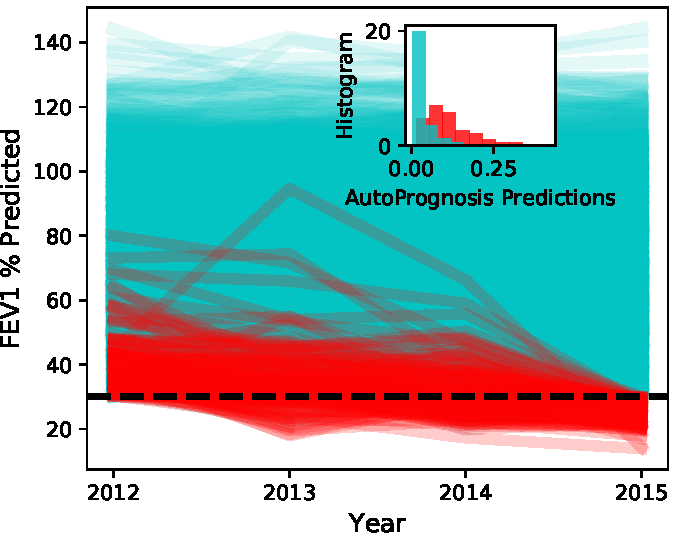
\includegraphics[width=2.75in]{ch6Fig3.pdf}
\caption{FEV$_1$ trajectories.}
\label{ch6fig3}
\end{minipage}%\hfill
\begin{minipage}[b]{0.45\linewidth}
\centering
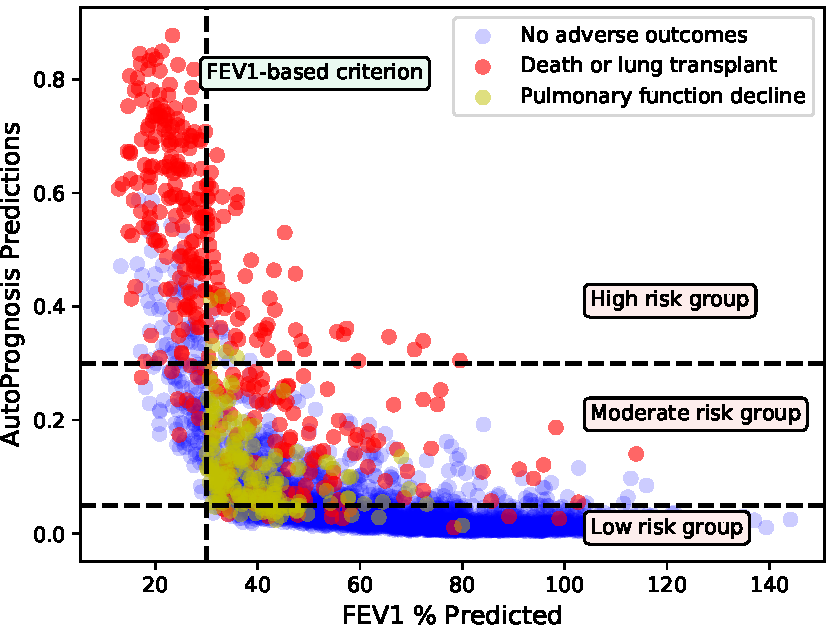
\includegraphics[width=2.85in]{ch6Fig4.pdf}
\caption{Predicted risk groups.}
\label{ch6fig4}
\end{minipage}
\end{figure}

The clinical utility of AutoPrognosis is not limited to transplant referral; the predictions prompted by AutoPrognosis serve as granular risk scores that can quantify the severity of future outcomes and hence can be used for treatment planning, follow-up scheduling, or estimating the time at which a transplant would be needed in the future. For instance, decisions on whether a CF patient carrying a G551D mutation should start taking the (expensive) ivacaftor or lumacaftor drugs can be guided by the predictions of our model \cite{rowe2014clinical,wainwright2015lumacaftor}. Patients with risk predictions that do not exceed the LT referral threshold are not equally healthy; higher risk scores are still indicative of higher levels of CF severity. The results in Tables \ref{ch6Table3} and \ref{ch6Table4} quantify the models' ability to distinguish patients with and without poor (binary) outcomes (death or LT), but do not show how well the different models are able to predict less severe outcomes. To this end, we sought to classify the predictions of AutoPrognosis into low, moderate and high risk categories, and test the model's ability to predict intermediate poor outcomes. We chose {\it pulmonary function decline} within a 3-year period as the intermediate poor outcome; we define pulmonary decline as the event when a patient has an FEV$_1 \%$ predicted less than 30$\%$ in the year 2015 (but did not undergo a lung transplant) when her FEV$_1 \%$ predicted was greater than 30$\%$ in 2012.   

The FEV$_1$ trajectories for all patients enrolled in the UK CF registry in 2012 are visualized in Figure \ref{ch6fig3}; FEV$_1$ trajectories corresponding to pulmonary decline events are highlighted in red. The trajectories in Figure \ref{ch6fig3} belong only to patients who had FEV$_1>30\%$ in 2012 and did not die or undergo a transplant in 2015. A total of 4.4$\%$ of those patients experienced pulmonary function decline in 2015. The inset plot in Figure \ref{ch6fig4} shows a histogram for the predictions of AutoPrognosis stratified by the occurrence of a pulmonary decline; we can visually see that AutoPrognosis is able to discriminate patients with and without the intermediate poor outcome. A two-sample $t$-test rejects the hypothesis that the average predictions for AutoPrognosis for patients with and without pulmonary decline are equal ($p$-value $< 0.0001$). The average predicted risk for patients without pulmonary decline was 0.046, whereas for those with pulmonary decline, the average predicted risk was 0.116. In order to assess the ability of our model to predict the pulmonary decline events, we redefined the poor outcomes as being death, lung transplant or pulmonary decline in a 3-year period. The in-sample average precision and AUC-PR of the predictive model learned by AutoPrognosis were 0.66 (95$\%$ CI: 0.63$-$0.69) and 0.65 (95$\%$ CI: 0.63$-$0.69), respectively, whereas those achieved by the model developed by Nkam {\it et. al} were 0.51 (95$\%$ CI: 0.48$-$0.54) and 0.48 (95$\%$ CI: 0.45$-$0.51). (95$\%$ confidence intervals were obtained via bootstrapping.) This demonstrates that AutoPrognosis is more precise than the existing models in predicting intermediate poor outcomes. 

Predicated on the results above, we classified the CF population into three risk groups, with low, moderate and high risk, based on the risk predictions of AutoPrognosis. (In what follows, we converted the outputs of AutoPrognosis, which are real numbers between 0 and 1, into percentages.) The risk groups are defined as follows: the low risk group is associated with risk predictions in the range (0-5$\%$), whereas the moderate risk group is associated with risk predictions in the range (5-30$\%$), and finally, the high risk group is associated with risk predictions that exceed 30$\%$. Figure \ref{ch6fig4} is a scatter plot for the CF patient outcomes in 2015 (red colored dots correspond to deaths or transplants, yellow dots correspond to pulmonary decline events, and blue dots correspond to patients with no adverse outcomes). The outcomes are plotted against the predictions issued by AutoPrognosis ($y$-axis), and every individual patient's FEV$_1$ measure in 2012 ($x$-axis). As we can see, the FEV$_1$ criterion can only provide a low-precision classification of patients with and without the poor outcome, whereas AutoPrognosis provides a more precise risk stratification for the CF population in which most patients with intermediate poor outcomes (pulmonary decline) reside in the moderate risk group, and patient allocation to the high risk group exhibits lower false alarm rates (refer to Table \ref{ch6Table4}). Clinicians can use the risk predictions and risk strata learned by AutoPrognosis as actionable information that guide clinical decisions. For instance, patients in the high risk group would be immediately referred to a transplant, patients in the moderate risk group would be recommended a drug with potential consideration for a transplant in the future, and patients in the low risk group should routinely pursue their next annual review.    

\begin{figure}[!htbp] %[h]
\begin{minipage}[b]{0.5\linewidth}
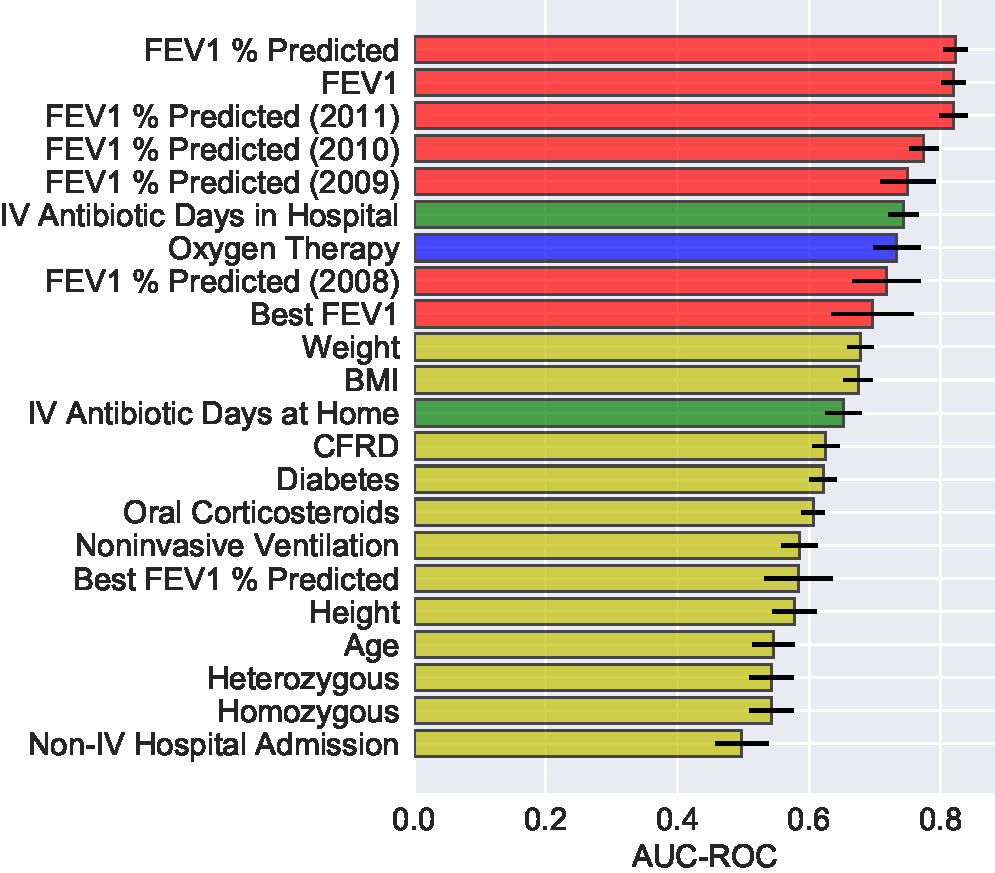
\includegraphics[width=3.25in]{ch6Fig5.pdf}
\caption{\small AUC-ROC of individual variables.}
\label{ch6fig5}
\end{minipage}\hfill
\begin{minipage}[b]{0.5\linewidth}
\centering
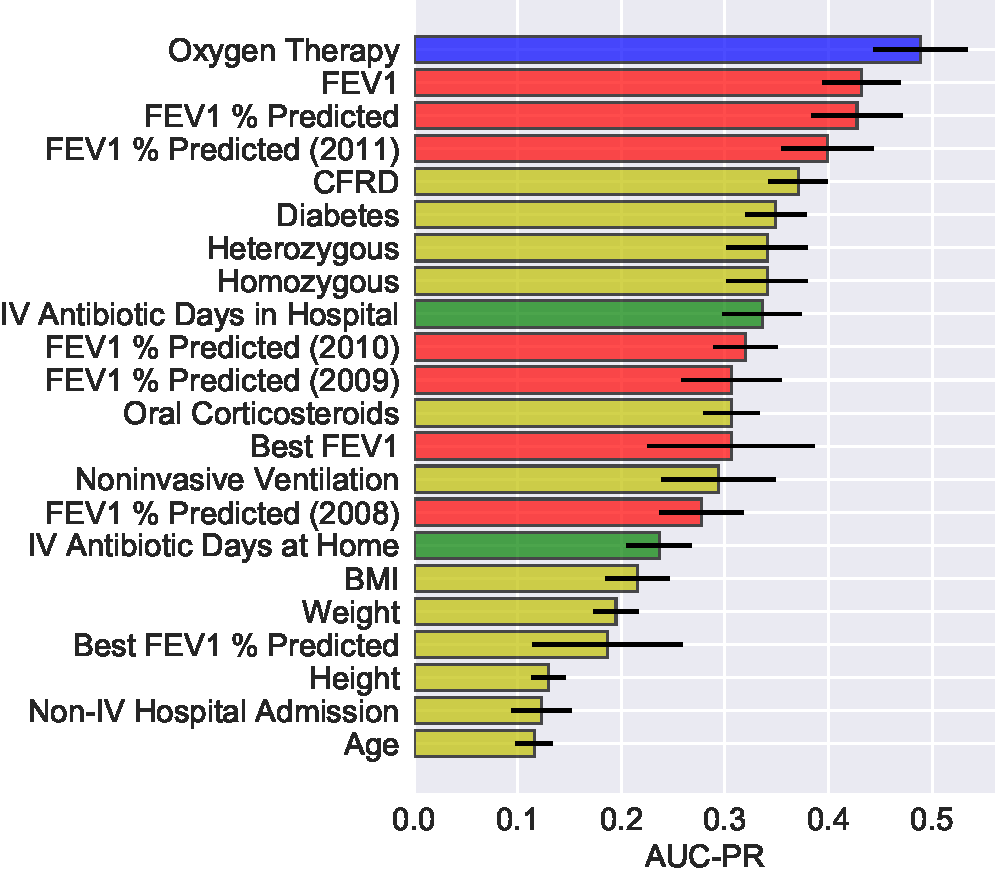
\includegraphics[width=3.25in]{ch6Fig6.pdf}
\caption{\small AUC-PR of individual variables.}
\label{ch6fig6}
\end{minipage}
\end{figure}

\subsection{Variable Importance Analysis} 

We sought to understand how the different patient variables contribute to the predictions issued by AutoPrognosis. Previous studies have identified a wide range of CF risk factors including FEV$_1 \%$ predicted\cite{liou2005use,aaron2015statistical,mccarthy2013cf,nkam20173,szczesniak2017phenotypes}, female gender\cite{aaron2015statistical,szczesniak2017phenotypes}, BMI\cite{mccarthy2013cf,dimitrov2015cf}, Pseudomonas Aeruginosa infection\cite{aaron2015statistical}, Burkholderia cepacia colonization\cite{nkam20173}, hospitalization\cite{nkam20173}, CF-related diabetes\cite{chamnan2010diabetes,szczesniak2017phenotypes}, non-invasive ventilation\cite{nkam20173}, and $\Delta$F508 homozygous mutation\cite{aaron2015statistical}. Since AutoPrognosis was trained in order to provide precise predictions, we focus not only on identifying variables that are most predictive of the outcomes in the sense of AUC-ROC maximization, but also on understanding which variables AutoPrognosis exploited in order to improve the precision (i.e. PPV) of the learned model (refer to Tables \ref{ch6Table3} and \ref{ch6Table4}). These variables can then be considered when updating the current consensus guidelines on LT referral and waiting list priority allocation \cite{weill2015consensus}. 

We evaluated the predictive power of each individual variable by providing AutoPrognosis with one variable at a time, and assessing the diagnostic accuracy of the model that it constructs using only that variable. We evaluated the AUC-ROC and the AUC-PR metrics (using 10-fold stratified cross-validation) in order to get a full picture of each variable's predictive power with respect to sensitivity, specificity, precision and recall. The most predictive 22 variables with respect to both the AUC-ROC and the AUC-PR metrics are illustrated in Figures \ref{ch6fig5} and \ref{ch6fig6}. In both figures, the bars associated with the variables correspond to the AUC-ROC/AUC-PR performance achieved by AutoPrognosis using only this variable. The black error bars correspond to the 95$\%$ confidence intervals. Since CF patients may encounter pulmonary disorders manifesting in either increased {\it airway resistance} or impaired {\it gas exchange} \cite{young2011gas}, we labeled the patients' variables in Figures \ref{ch6fig5} and \ref{ch6fig6} based on the aspect of lung function that they reflect. Variables that describe lung function in terms of airway resistance (e.g. FEV$_1$, FEV$_1 \%$ predicted, FEV$_1$ trajectory, etc) are represented through red bars. Variables that describe lung function in terms of gas exchange (e.g. Oxygenation) are represented through blue bars. Variables that represent pulmonary disorders resulting from bacterial infections are represented through green bars. All other variables had their corresponding bars colored in yellow. 

Figure \ref{ch6fig5} shows that the spirometric (FEV$_1$) biomarkers, including the FEV$_1$ measurements collected 3 years prior to 2012, display the best AUC-ROC performance. Interestingly, we found that the history of FEV$_1$ measurements (e.g. the FEV$_1\%$ predicted 1 year before baseline) is as predictive as the FEV$_1$ measurements at baseline. Variables reflecting pulmonary disorders resulting from bacterial infections (intravenous antibiotic courses in hospital\cite{ewence2017302}) were the second most predictive in terms of the AUC-ROC performance. The most predictive complications were found to be diabetes and CF-related diabetes. Apart from intravenous antibiotics, the most predictive treatment-related variable was usage of oral corticosteroids. Genetic variables and microbiological infections were found to have a poor predictive power when used solely for predictions, though intravenous antibiotic courses can be thought of as proxies for microbiological infections.  

Figure \ref{ch6fig6} shows that the importance ranking for the patients' variables changes significantly when using precision (i.e. AUC-PR) as a measure of the variables' predictive power. Most remarkably, reception of Oxygen therapy turns out to be the variable with the highest AUC-PR. Hence, precise risk assessment and transplant referral decisions need to consider, in addition to the spirometric biomarkers, other biomarkers that reflect disorders in gas exchange, such as the partial pressure of carbon dioxide in arterial blood ($\mbox{PaCO}_2$) and Oxygen saturation by pulse oximetry ($\mbox{SpO}_2$) \cite{sheikh2011severe}. Prevalence of respiratory failures that are usually treated via Oxygenation, such as hypoxemia and hypercapnia\cite{sheikh2011severe,hetero,young2011gas,wojewodka2014candidate}, should be considered as decisive criteria for LT referral even when airway obstruction is not severe (i.e. FEV$_1>$30$\%$). AutoPrognosis was able to learn a prediction rule that carefully combines spirometric and gas exchange variables in order to come up with a precise lung transplant referral criterion that accurately disentangles patients who are truly at risk from those who do not need a lung in the near future (refer to Tables \ref{ch6Table3} and \ref{ch6Table4}). Our results indicate that looking at the right accuracy metric that reflects the true clinical utility (in this case the precision-recall curve) is important not only for tuning and comparing predictive models, but also for discovering risk factors that are relevant for clinical decision-making.          

\begin{figure}[t]
\centering
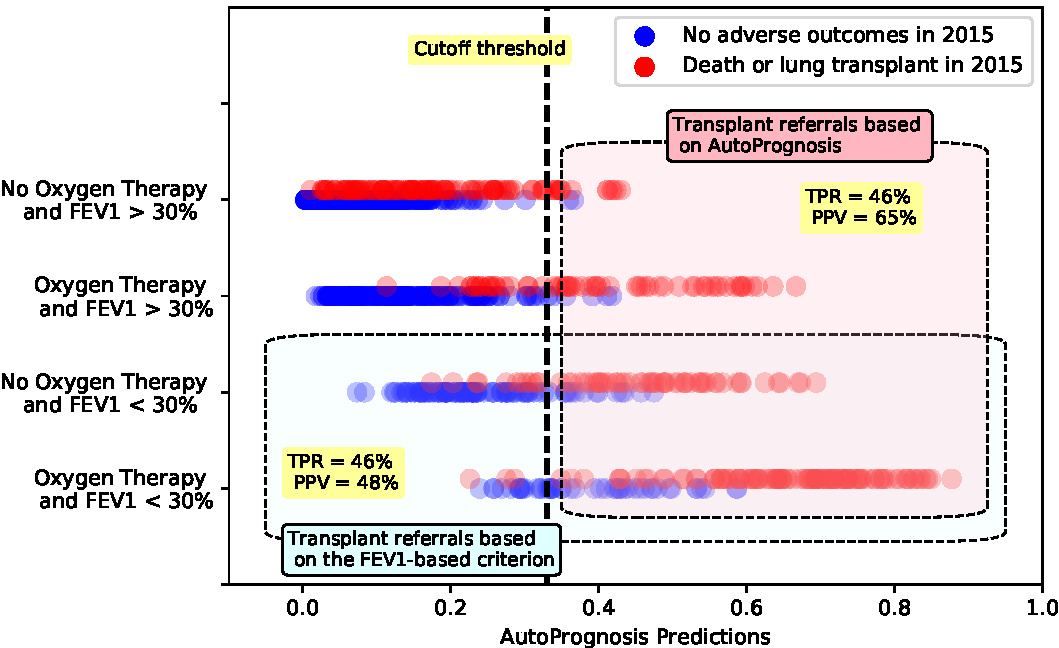
\includegraphics[width=5in]{ch6Fig7.pdf}
\caption{Depiction for transplant referral policies based on AutoPrognosis and the FEV$_1$ criterion for different patient subgroups.}
\label{ch6fig7}
\end{figure}

Figures \ref{ch6fig7} illustrates how LT referral policies based on AutoPrognosis handle patient subgroups stratified by spirometric and Oxygenation variables. In this Figure, we look at 4 subgroups: patients with FEV$_1<30\%$ who received Oxygen therapy, patients with FEV$_1<30\%$ who did not receive Oxygen therapy, patients receiving Oxygen therapy but had FEV$_1\geq 30\%$, and patients who were neither Oxygenated nor had their FEV$_1$ drop below the 30$\%$ threshold. The subgroup memberships are labeled on the $y$-axis; every patient is represented as a dot in a scatter plot, with the $x$-axis quantifying the risk estimate of AutoPrognosis for every individual patient. Patients with adverse outcomes are represented via red dots, whereas those with no adverse outcomes are depicted as blue dots. As we can see in Figure \ref{ch6fig7}, the simple FEV$_1$ criterion would refer the two subgroups with poor spirometric biomarkers (FEV$_1<30\%$) to a transplant; this leads to a referral list with many blue dots (this is depicted via the dotted box that groups all patients with FEV$_1<30\%$ in Figure \ref{ch6fig7}), and consequently a high false positive rate that leads to a PPV of 48$\%$. Contrarily, AutoPrognosis orders the risks of the 4 subgroups by accounting for both Oxygenation and spirometry; this results in a more precise list of referrals at any given cutoff threshold (as can be seen in the dotted box that groups all patients with risk cutoff of 0.33, where the majority of the dots in the box are red). AutoPrognosis achieves precision by assigning a high risk to Oxygenated patients, even if their spirometric biomarkers are not severe. At a fixed TPR of 46$\%$, this leads to some patients with FEV$_1<30\%$ but good clinical outcomes being replaced with Oxygenated patients with FEV$_1>30\%$ who experienced adverse outcomes, which raises the PPV to 65$\%$.

\section{Discussion and Conclusions}
In this Chapter, we applied the AutoPrognosis framework, developed earlier in Chapter 4, to the problem of predicting short-term survival of cystic fibrosis patients using data from the UK CF registry. AutoPrognosis was capable of learning an ensemble of machine learning models (including the well-known random forest and XGBoost algorithms) that outperformed existing risk scores developed in the clinical literature, mainstream practice guidelines, and na\"ive implementation of vanilla machine learning models. We demonstrated the clinical utility of the prognostic model learned by AutoPrognosis by examining its potential impact on lung transplant referral decisions. Our analysis showed that the model learned by AutoPrognosis achieves significant gains in terms of a wide variety of diagnostic accuracy metrics. Most notably, AutoPrognosis achieves significant gains in terms of the positive predictive values, which implies a remarkable improvement in terms of the precision of lung transplant referral decisions. AutoPrognosis' interpreter module revealed that the model is able to achieve such gains because it recognizes the importance of variables that reflect disorders in pulmonary gas exchange (such as Oxygenation), and learns their interactions with spirometric biomarkers reflecting airway obstruction (such as FEV$_1$). This gave rise to a precise survival prediction rule which disentangles patients who are truly at risk from those who do not necessarily need a transplant in the short term.

Although our study provided empirical evidence for the clinical usefulness of applying automated machine learning in prognostication, it has some limitations. First, the prognostic model learned by AutoPrognosis needs to be externally validated in order to ensure that our findings generalize to other CF populations. Second, the net clinical utility of our model needs to be evaluated by considering post-transplant survival data, through which we can identify high-risk patients for whom a transplant is indeed beneficial. Finally, we had no access for data on patients who went through a transplant evaluation process or were enrolled in wait list but did not get a transplant within the 3-year analysis horizon, which rendered direct comparisons with the actually realized clinical policy impossible.


\chapter{Cardiovascular Disease Risk Prediction}
\section{Background}
\label{ch7sec0}
Globally, cardiovascular disease (CVD) remains the leading cause of morbidity and mortality \cite{thomas2017novel}. Current guidelines for primary prevention of CVD emphasize the need to identify asymptomatic patients who may benefit from preventive action (e.g., initiation of statin therapy \cite{ridker2008rosuvastatin}) based on their predicted risk \cite{kremers2008high,d2008general,conroy2003estimation,sjostrom2004lifestyle}. Different guidelines recommend different algorithms for risk prediction. For example, the 2010 American College of Cardiology/American Heart Association (ACC/AHA) guideline \cite{greenland20102010} recommended use of Framingham Risk Score \cite{d2008general}, whereas the 2016 European guidelines recommended use of the Systematic Coronary Risk Evaluation (SCORE) algorithm \cite{piepoli20162016}. In the UK, the current National Institute for Health and Care Excellence (NICE) guidelines recommend use of the QRISK2 score to guide the initiation of lipid lowering therapies \cite{hippisley2008predicting,hippisley2017development}. 

Existing CVD risk scores are typically developed using multivariate regression models that combine information on a limited number of well-established risk factors, and generally assume that all such factors are related to the CVD outcomes in a linear fashion, with limited or no interactions between the different factors. Because of their restrictive modeling assumptions and limited number of predictors, existing algorithms generally exhibit modest predictive performance \cite{siontis2012comparisons}, especially for certain sub-populations such as individuals with diabetes \cite{coleman2007framingham,mcewan2004evaluating,martin2014type,buse2007primary} or rheumatoid arthritis \cite{kremers2008high}. Data-driven techniques based on machine learning (ML) can improve the performance of risk predictions by exploiting large data repositories to agnostically identify novel risk predictors and more complex interactions between them. However, only a few studies have investigated the potential advantages of using ML approaches for CVD risk prediction, focusing only on a limited number of ML methods \cite{ambale2017cardiovascular,ahmad2018machine} or a limited number of risk predictors \cite{weng2017can}.   

In this Chapter, we explore the potential value of using ML approaches to derive risk prediction models for CVD. We analyzed data on 423,604 participants without CVD at baseline in UK Biobank, a large prospective cohort study in which participants were recruited from 22 centers throughout the UK. Similar to the previous Chapter, we used the AutoPrognosis framework --- developed in Chapter 4 --- to derive an ML-based CVD risk prediction model and evaluated its predictive performances in the overall population and clinically relevant sub-populations. 

\section{Data and Experimental Setup}
\label{ch7sec1}
\subsection{Study Design and Participants}
Participants were enrolled in the UK Biobank from 22 assessment centers across England, Wales, and Scotland, during the period spanning from 2006 to 2010 \cite{sudlow2015uk}. We extracted a cohort of participants who were 40 years of age or older and had no known history of CVD at baseline. That is, patients with previous history of coronary heart disease, other heart disease, stroke, transient ischaemic attack, peripheral arterial disease, or cardiovascular surgery were excluded from the analysis. The total number of participants who met the inclusion criteria was 423,604. The last available date of participant follow-up was Feb 17, 2016. UK Biobank obtained approval from the North West Multi-centre Research Ethics Committee (MREC), and the Community Health Index Advisory Group (CHIAG). All participants provided written informed consent prior to enrollment in the study. The UK Biobank protocol is available online \cite{palmer2007uk}.  

The UK Biobank dataset keeps track of a large number of variables for each participant, but most of those variables are missing for most patients. In order to include the maximum possible number of (informative) variables in our analysis, we included all variables that are missing for less than 50$\%$ of patients with CVD outcomes. This corresponded to a rate of missingness of 85$\%$ for the entire population of participants. Our rationale for assessing the missingness rate among patients with CVD is that missingness itself maybe informative (i.e., the chance of a variable being missing may depend on the outcome). By excluding all variables that were missing for more than 85$\%$ of the participants, a total of 473 variables were included in our analysis. We categorized all variables in the UK Biobank into 9 categories: health and medical history, lifestyle and environment, blood assays, physical activity, family history, physical measures, psychosocial factors, dietary and nutritional information, and sociodemographics \cite{ganna20155}.
 

\subsection{Outcome}
The primary outcome was the first fatal or non-fatal CVD event. A CVD event was defined as the assignment of any of the ICD-10 diagnosis codes F01 (vascular dementia), I20-I25 (coronary/ischaemic heart diseases), I50 (heart failure events, including acute and chronic systolic heart failures), and I60-I69 (cerebrovascular diseases), or any of the ICD-9 codes 410-414 (ischemic heart disease), 430-434, and 436-438 (cerebrovascular disease). Follow-up data was obtained from the hospital episode statistics (a data warehouse containing records of all patients admitted to NHS hospitals), and the equivalent datasets in Scotland and Wales \cite{adamska2015challenges}.  

\subsection{Characteristics of the Study Population}
A total of 423,604 participants had sufficient information for inclusion in this analysis. Overall, the mean (SD) age of participants at baseline was 56.4 (8.1) years, and 188,577 participants (44.5$\%$) were male. Over a median follow-up of 7 years (5th-95th percentile: 5.7-8.4 years; 3 million person-years at risk), there were 6,703 CVD cases. The mean age of CVD cases was 60.5 years (60.2 years for men and 61.1 years for women). Because the minimum follow-up period for all participants was 5 years, we evaluated the accuracy of the different models in predicting the 5-year risk of CVD. At a 5-year horizon, the total number of CVD cases was 4,801.

\subsection{Models Tested}

\subsubsection*{Framingham Risk Score}
At the time of conducting this study, the UK Biobank had not yet released data on the participants' total cholesterol, HDL cholesterol and LDL cholesterol, which are used as predictors in various established algorithms, such as Framingham score \cite{d2008general}, ACC/AHA \cite{goff20142013}, QRISK2 \cite{hippisley2008predicting}, and SCORE \cite{conroy2003estimation}. The Framingham score, however, provides an incarnation of its underlying model based on nonlaboratory predictors, which replaces lipids with Body Mass Index (BMI) \cite{d2008general}. Since BMI is currently collected for 99.38$\%$ of the UK Biobank participants, we compared our model with the BMI version of the Framingham score. We used the published predicting equations (beta-coefficients and survival functions) of the BMI-based Framingham model developed in \cite{d2008general}. (Framingham risk calculator and model coefficients are publicly available in: \href{https://www.framinghamheartstudy.org/fhs-risk-functions/cardiovascular-disease-10-year-risk/}{https://www.framinghamheartstudy.org}.) 

The Framingham score is based on 7 core risk factors: gender, age, systolic blood pressure, treatment for hypertension, smoking status, history of diabetes, and BMI. All of those variables were complete for the participants in the extracted cohort, with the exception of systolic blood pressure (missing for 6.8$\%$ of the participants), and BMI (missing for 0.62$\%$ of the participants). We used the {\it MissForest} non-parametric data imputation algorithm \cite{stekhoven2011missforest} to recover the missing values. Using the MissForest algorithm, we sampled 5 imputed datasets and averaged the model predictions for each participant on the 5 datasets (this is known in the literature as Rubin's rules \cite{stekhoven2011missforest}). The number of imputed datasets was selected via cross-validation.  
 
\subsubsection*{Cox Proportional Hazards Model}
We evaluated the performance of two Cox Proportional Hazards (PH) models derived from the analysis cohort: a model that only uses the traditional 7 risk factors used by the Framingham score, and a model that uses all of the 473 variables in the UK Biobank. To fit the Cox PH models, we imputed the missing data using the MissForest imputation algorithm (with 5 imputations). The Cox PH model that uses the traditional 7 risk factors used by Framingham score can be thought of as a variant of Framingham score calibrated to the UK population (the Framingham score was originally derived for a US population). For the Cox PH model that uses all of the 473 predictors, we applied variable selection using the LASSO method \cite{tibshirani1996regression}. (Variable selection was applied since fitting the Cox model with all variables resulted in an inferior performance due to the numerical collapse of the Cox model solvers in high dimensions.) To apply variable selection, we fit a LASSO regression model (a linear model penalized with the L1 norm) to predict the (binary) CVD outcomes. The fitted model gives a sparse solution whereby many of the estimated coefficients are zero. We select all the variables with non-zero coefficients in the fitted LASSO model and feed those variables into a Cox model fitted on the same batch of data. We optimize the LASSO model regularization parameter via cross-validation. 

\section{Model Development using AutoPrognosis}
\label{ch7sec2}
\subsection*{Model Training}
To train the AutoPrognosis model, we conduct 200 iterations of the Bayesian optimization procedure in presented in Chapter 4, where in each iteration the algorithm explores a new ML pipeline and tunes its hyper-parameters. Cross-validation was used in every iteration to evaluate the performance of the pipeline under evaluation. The (in-sample) model learned by AutoPrognosis combined 200 weighted ML pipelines, the strongest of which comprised the MissForest data imputation algorithm, no feature processing steps, an {\it XGBoost} ensemble classifier (with 200 estimators) \cite{chen2016xgboost}, and sigmoid regression for calibration. 

\subsection*{Variable Ranking}
In order to identify the relative importance of the 473 variables used to build our model, we use a {\it post-hoc} approach to rank the contribution of the different variables in the predictions issued by the model. The ranking is obtained by fitting a random forest model with the participants' variables as the inputs, and the predictions of our model as the outputs, and then assigning variable importance scores to the different variables using the standard permutation method in \cite{strobl2008conditional}. Using the permutation method, we assess the mean decrease in classification accuracy for every variable after permuting that variable over all trees. The resulting variable importance scores reflect the impact each variable has on the predictions issued by AutoPrognosis. We used the random forest algorithm for post-hoc variable ranking because it is a nonparametric algorithm that can recognize complex patterns of variable interaction while enabling principled evaluation of variable importance \cite{strobl2008conditional}. Other variable ranking methods based on associative classifiers (such as the one proposed in \cite{alaa2018autoprognosis}) entail a computational complexity that is exponential in the number of variables, and hence are not suitable for our study as it involves more than 400 variables. 

To disentangle the ``modeling gain'' achieved by utilizing ML-based techniques from the ``information gain'' achieved by just using more variables, we created a simpler version of AutoPrognosis that only uses the same 7 core risk factors (age, gender, systolic blood pressure, smoking status, treatment of hypertension, history of diabetes, and BMI) used by the existing prediction algorithms. In addition, we created another version of the AutoPrognosis model that uses only non-laboratory variables in UK Biobank.

\subsection*{Statistical Analysis}
In order to avoid over-fitting, we evaluated the prediction accuracy of all models under consideration via 10-fold stratified cross-validation using area under the receiver operating characteristic curve (AUC-ROC). In every cross-validation fold, a training sample (381,244 participants) was used to derive the Cox PH models, standard ML models, and our model (AutoPrognosis), and then a held-out sample (42,360 participants) was used for performance evaluation. We report the mean AUC-ROC and the 95$\%$ confidence intervals (Wilson score intervals) for all models. The calibration performance of our model was evaluated via the Brier score. 

\begin{table}[t]
\centering
\begin{tabular}{|c|c|c|}
\hline
{\bf \footnotesize Model} & {\bf \footnotesize AUC-ROC} & {\bf \footnotesize Absolute AUC-ROC Change}  \\ \hline
{\footnotesize Framingham score} & {\footnotesize 0.724 $\pm$ 0.004} & {\footnotesize Baseline model}  \\ \hline 
{\footnotesize Cox PH Model (7 core variables)} & {\footnotesize 0.734 $\pm$ 0.005} & {\footnotesize + 1.0$\%$}  \\ \hline 
{\footnotesize Cox PH Model (all variables)} & {\footnotesize 0.758 $\pm$ 0.005} & {\footnotesize + 3.4$\%$} \\ \hline\hline
{\footnotesize AutoPrognosis (7 core variables)} & {\footnotesize 0.744 $\pm$ 0.005} & {\footnotesize + 2.0$\%$}   \\ \hline
{\footnotesize AutoPrognosis (369 non-lab. variables)} & {\footnotesize 0.761 $\pm$ 0.005} & {\footnotesize + 3.7$\%$}    \\ \hline
{\footnotesize AutoPrognosis (104 lab. variables)} & {\footnotesize 0.735 $\pm$ 0.008} & {\footnotesize + 1.1$\%$}  \\ \hline
{\footnotesize AutoPrognosis (all variables)} & {\footnotesize 0.774 $\pm$ 0.005} & {\footnotesize + 5.0$\%$} \\ \hline
\end{tabular}
\caption{Performance of different CVD risk prediction models.}
\label{ch7Table1}
\end{table}

\begin{table}[t]
\centering
\begin{tabular}{|c|c|c|c|}
\hline
{\bf \footnotesize Variable (Men)} & {\bf \footnotesize Score} & {\bf \footnotesize Variable (Women)} & {\bf \footnotesize Score} \\ \hline
{\footnotesize {\bf \underline{A}g\underline{e}$^{*}$}} & {\footnotesize 0.346} & {\footnotesize {\bf \underline{A}g\underline{e}$^{*}$}} & {\footnotesize 0.370}   \\ \hline
{\footnotesize {\bf \underline{Smokin}g$^{*}$}} & {\footnotesize 0.101} & {\footnotesize {\bf \underline{Smokin}g$^{*}$}} & {\footnotesize 0.099}  \\ \hline
{\footnotesize Usual walking pace} & {\footnotesize 0.052} & {\footnotesize Usual walking pace} & {\footnotesize 0.057}  \\ \hline
{\footnotesize {\bf \underline{S}y\underline{stolic blood} p\underline{ressure}$^{*}$}} & {\footnotesize 0.040}  & {\footnotesize Ankle spacing width} & {\footnotesize 0.035} \\ \hline
{\footnotesize Microalbumin in urine} & {\footnotesize 0.032} & {\footnotesize Self-reported health rating} & {\footnotesize 0.030}  \\ \hline
{\footnotesize High blood pressure} & {\footnotesize 0.030} & {\footnotesize {\bf \underline{S}y\underline{stolic blood} p\underline{ressure}$^{*}$}} & {\footnotesize 0.026}  \\ \hline
{\footnotesize Red blood cell distribution width} & {\footnotesize 0.025} & {\footnotesize High blood pressure} & {\footnotesize 0.024} \\ \hline
{\footnotesize Self-reported health rating} & {\footnotesize 0.019}  & {\footnotesize Red blood cell distribution width} & {\footnotesize 0.023} \\ \hline
{\footnotesize Haematocrit percentage} & {\footnotesize 0.014} & {\footnotesize Microalbumin in urine} & {\footnotesize 0.017}  \\ \hline
{\footnotesize Father age at death} & {\footnotesize 0.014} & {\footnotesize Father age at death} & {\footnotesize 0.017} \\ \hline
{\footnotesize {\bf \underline{BMI}$^{*}$}} & {\footnotesize 0.013} & {\footnotesize White blood cell count} & {\footnotesize 0.011} \\ \hline
{\footnotesize Diastolic blood pressure} & {\footnotesize 0.012} & {\footnotesize Number of Treatments} & {\footnotesize 0.011} \\ \hline
{\footnotesize White blood cell count} & {\footnotesize 0.012} & {\footnotesize Mean reticulocyte volume} & {\footnotesize 0.008} \\ \hline
{\footnotesize Impedance of arm (left)} & {\footnotesize 0.009} & {\footnotesize Leg predicted mass (right)} & {\footnotesize 0.006} \\ \hline
{\footnotesize Haemoglobin concentration} & {\footnotesize 0.007} & {\footnotesize Neutrophill count} & {\footnotesize 0.006} \\ \hline 
{\footnotesize Neutrophill count} & {\footnotesize 0.005} & {\footnotesize Basal metabolic rate} & {\footnotesize 0.005} \\ \hline
{\footnotesize Number of Treatments} & {\footnotesize 0.004} & {\footnotesize Hormone-replac. therapy usage} & {\footnotesize 0.005} \\ \hline
{\footnotesize Mean reticulocyte volume} & {\footnotesize 0.004} & {\footnotesize Blood clot in the leg} & {\footnotesize 0.004} \\ \hline 
{\footnotesize Urinary sodium concentration} & {\footnotesize 0.004} & {\footnotesize Forced expiratory volume} & {\footnotesize 0.004} \\ \hline
{\footnotesize Monocyte count} & {\footnotesize 0.004} & {\footnotesize Duration of fitness test} & {\footnotesize 0.004} \\ \hline 
\end{tabular}
\caption{Variable ranking by their contribution to the predictions of AutoPrognosis.}
\label{ch7Table2}
\end{table}

\section{Results}
\label{ch7sec3}

\subsection*{Prediction Accuracy}
\subsubsection*{Comparison of Prediction Models} 
The prediction accuracy of the different models under consideration evaluated at a 5-year horizon is shown in Table \ref{ch7Table1}. We used the Framingham score as a baseline model for performance evaluation (AUC-ROC: 0.724, 95$\%$ CI: 0.720-0.728). Both the Cox PH model with the 7 conventional risk factors (AUC-ROC: 0.734, 95$\%$ CI: 0.729-0.739), and the Cox PH model with all variables (AUC-ROC: 0.758, 95$\%$ CI: 0.753-0.763) achieved an improvement in the AUC-ROC compared to the baseline model ($p <$ 0.001). The improvement achieved by the Cox PH model that uses the same predictors used by the Framingham score is due in part to the fact that the Cox PH model is directly derived from the analysis cohort, whereas the Framingham score coefficients were derived from a different population. 

Most of the variables in the UK Biobank are non-laboratory variables collected through an automated touchscreen questionnaire about lifestyle, clinical history and nutritional habits. We evaluated the accuracy of AutoPrognosis once when it is trained with 369 variables corresponding to the participants' self-reported information (questionnaires) only, and once when it is trained with 104 variables obtained from blood assays, diagnostic tests, and physiological measurements. As we can see in Table \ref{ch7Table1}, AutoPrognosis with only questionnaire-related variables still achieves a significant improvement over the baseline Framingham score (AUC-ROC: 0.752, 95$\%$ CI: 0.747-0.757, $p <$ 0.001), and is superior to the model that only uses laboratory-based variables. 

\subsubsection*{Classification Analysis} 
In order to better assess the clinical significance of our results, we compared the AutoPrognosis model with the traditional Framingham score in predicting 7.5$\%$ CVD risk (threshold for initiating lipid-lowering therapies recommended by the NICE guidelines \cite{hippisley2017development}). At this operating point, the Framingham baseline model predicted 2,989 CVD cases correctly from 4,801 total cases, resulting in a sensitivity of 62.2$\%$ and PPV of 1.5$\%$. Our AutoPrognosis model correctly predicted 3,357 out of the 4,801 CVD cases, resulting in a sensitivity of 69.9$\%$ and PPV of 2.6$\%$. This corresponds to 368 net increase in the number of CVD patients who would benefit from receiving a preventive treatment in a timely manner when utilizing the predictions of our model.

\begin{table}[t]
\centering
\begin{tabular}{|c|c|c|}
\hline
{\bf \footnotesize Model} & {\bf \footnotesize AUC-ROC (No diabetes)} & {\bf \footnotesize AUC-ROC (Diabetes)}  \\ \hline
{\footnotesize Framingham score} & {\footnotesize 0.724 $\pm$ 0.004} & {\footnotesize 0.578 $\pm$ 0.018}  \\ \hline \hline
{\footnotesize AutoPrognosis} & {\footnotesize 0.774 $\pm$ 0.005} & {\footnotesize 0.713 $\pm$ 0.010} \\ \hline
\end{tabular}
\caption{Performance of AutoPrognosis in the diabetic patient subgroup.}
\label{ch7Table3}
\end{table}

\subsubsection*{Variable Importance} 
Table \ref{ch7Table2} lists the 20 most important variables ranked according to their contribution to the predictions of the AutoPrognosis model (along with their importance scores). Variables related to physical activity (usual walking pace) and information on blood measurements appeared to be more important for the predictions of AutoPrognosis than traditional risk factors included in most existing scoring systems. For women, a remarkable predictor of CVD risk was the measured ``ankle spacing width''. This may be linked to symptoms of poor circulation, such as swollen legs, which is predictive of future CVD events \cite{allison2008high}. We also found that usage of hormone-replacement therapy (HRT) was on the list of top predictors of CVD risk for women. For men, blood measurements such as haematocrit percentage and haemoglobin concentration, and variables such as urinary sodium concentration were among the most important risk factors.

\subsubsection*{Prediction Accuracy in Individuals with History of Diabetes} 
Among the 423,604 participants included in our cohort, a total of 17,908 participants (4.22$\%$) had a known history of diabetes (either Type 1 or Type 2) at baseline. In Table \ref{ch7Table3}, we show the AUC-ROC performance of AutoPrognosis and the baseline Framingham score when validated separately on the diabetic and non-diabetic populations. As we can see, the baseline Framingham score was less accurate in the diabetic population (AUC-ROC: 0.578, 95$\%$ CI: 0.560-0.596) compared to its achieved accuracy for the overall population (AUC-ROC: 0.724, 95$\%$ CI: 0.720-0.728, $p <$ 0.001). On the contrary, AutoPrognosis maintained high predictive accuracy for the diabetic population (AUC-ROC: 0.713, 95$\%$ CI: 0.703-0.723).

We note that the list of important variables in the diabetic subgroup is substantially different from that of the overall population. One major difference is that for diabetic patients, microalbuminuria appeared to be strongly linked to an elevated CVD risk. In the overall population (423,604 participants), the average measure of microalbumin in urine was 27.8 mg/L for participants with no CVD events, and 52.2 mg/L for participants with CVD events. In the diabetic population (17,908 participants), participants with no CVD events had an average microalbumin in urine of 61.0 mg/L, whereas for those with a CVD event, the average microalbumin in urine was 128.76 mg/L. (Information on microalbumin in urine was available for 30$\%$ of the patients in the overall population, and 50$\%$ of patients in the diabetic population.) 

\subsubsection*{Predictive Ability of Individual Variables in UK Biobank} 
In order to evaluate the individual predictive ability of the UK Biobank variables, we exhaustively fitted simple versions of our AutoPrognosis model for each of the 473 variables. For each such model, we use one distinct variable as an input and evaluate the resulting AUC-ROC. Because most variables are correlated with age and gender, we use the age variable as a second predictor for all models, and fit separate models for men and women. The AUC-ROC values of the resulting models are depicted in the scatter-plot in Fig \ref{ch7fig1}.    

\begin{figure}[t]
\centering
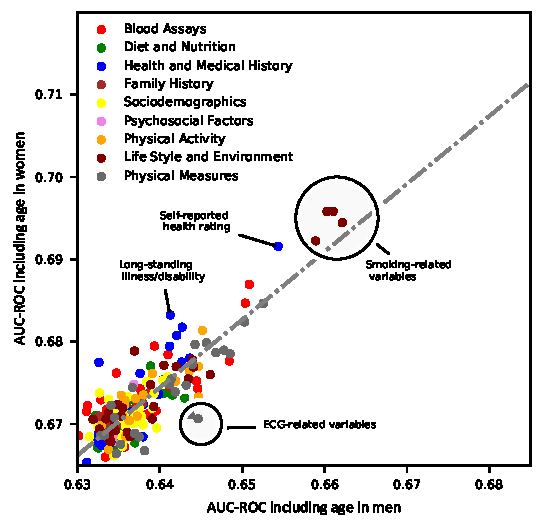
\includegraphics[width=5in]{ch7Fig1.pdf}
\caption{{\bf Predictive ability of the UK Biobank variables for men and women.} Each point represents a variable in the UK Biobank ordered by the ability to predict CVD events for men and women. Predictions based solely on age achieved an AUC-ROC of 0.632 $\pm$ 0.003 for men and 0.665 $\pm$ 0.002 for women. We report the AUC-ROC from models trained with individual variables in addition to age, and only display variables that achieved a statistically significant improvement in AUC-ROC compared to predictions based on age only. Each color represents a different variable category. Variables deviating from the (dotted gray) regression line have an AUC-ROC that differs between men and women more than expected in view of the overall association between the two genders, suggesting a stronger relative importance in one gender group.}
\label{ch7fig1}
\end{figure}
As shown in Fig \ref{ch7fig1}, variables related to smoking habits or exposure to tobacco smoke displayed the highest predictive ability. Self-reported health rating was predictive for both genders, but more predictive for women. Existence of long-standing illness was strongly predictive of CVD events for women, and less predictive for men. Variables extracted from the electrocardiogram (ECG) records possessed stronger predictive ability for men.  

\section{Discussion and Conclusions}
In this large prospective cohort study, we developed a ML model based on the AutoPrognosis framework for predicting CVD events in asymptomatic individuals. The model was built using data for more than 400,000 UK Biobank participants, with over 450 variables for each participant. Our study conveys several key messages. First, AutoPrognosis significantly improved the accuracy of CVD risk prediction compared to well-established scoring systems based on conventional risk factors and currently recommended by primary prevention guidelines (Framingham score). Second, AutoPrognosis was able to agnostically discover new predictors of CVD risk. Among the discovered predictors were non-laboratory variables that can be collected relatively easily via questionnaires, such as the individuals' self-reported health ratings and usual walking pace. Third, AutoPrognosis uncovered complex interaction effects between different characteristics of an individual, which led to recognition of risk predictors that are specific to certain sub-populations for whom existing guidelines were providing unreliable predictions. 

\subsection*{When can ML help in prognostic modeling?}
The abundance of a large number of informative variables in the UK Biobank (473 variables) guarantees an ``information gain'' that can be achieved by any data-driven model, including the standard Cox PH model, compared to the existing prediction algorithms that use only a limited number of conventional risk factors (e.g., Framingham score). The results in Table \ref{ch7Table1} show that, in addition to the information gain, AutoPrognosis also attained a ``modeling gain'' that allowed it to outperform the standard Cox PH model that uses all of the 473 variables. In general, the modeling gain achieved by AutoPrognosis would result from its ability to select among different models with various levels of complexity and numerical robustness in a completely data-driven fashion, without committing to any presupposition about the superiority of any given model. In our experiments, the Cox PH supplied with all of the 473 variables (without variable selection) provided a noticeably poor performance (i.e., an average AUC-ROC of 0.6). This is because the numerical solvers of the Cox PH model collapse when the data dimensionality is very large --- this is why a variable selection pre-processing step was essential for fitting the Cox PH model. This implies that, even if the true underlying data model is perfectly linear, fitting standard linear models such as Cox PH or linear regression may not be sufficient for harnessing the information gain, since such models are not numerical robust in high-dimensional settings. AutoPrognosis solves this problem by selecting more robust models that better fit the high-dimensional data --- in our experiments, these where tree-based models such as XGBoost and random forests. This observation shows that information gain and modeling gain are inherently entangled: to harness the information gain, we need to consider a more complex modeling space.

While the information gain appeared to be more significant than the modeling gain in our experiments, we note that even when provided with the same 7 core risk factors used by the Framingham score, AutoPrognosis was still able to offer a statistically significant AUC-ROC gain compared to the Framingham score and a Cox PH model that uses the same 7 variables. This shows that the modeling gain is not necessarily limited to settings where many predictors are available and numerical robustness, but is rather achievable whenever a small number of predictors display complex interactions.    

\subsection*{Risk prediction with non-laboratory variables}
Individuals in developed countries tend to seek out health information through online resources and web-based risk calculators \cite{hesse2005trust}. In developing countries, where 80$\%$ of all world-wide CVD deaths occur \cite{gaziano2008laboratory}, there are limited resources for risk assessment strategies that require laboratory testing \cite{gaziano2008laboratory,mendis2007world}. The results in Table \ref{ch7Table1} show that AutoPrognosis could potentially provide reliable risk predictions by using information from non-laboratory variables about the participants' lifestyle and medical history. The most predictive non-laboratory variables included in our model were ages, gender, smoking status, usual walking pace, self-reported overall health rating, previous diagnoses of high blood pressure, income, Townsend index and parents' ages at death. Inclusion of such variables in web-based risk calculators can help provide reasonably accurate risk predictions when obtaining laboratory variables is not viable.

One remarkable finding in Table \ref{ch7Table1} (and Fig \ref{ch7fig1}) is that apart from the well-established age and gender risk factors, two other non-laboratory variables were found to be very predictive of the CVD outcomes; those are the ``self-reported health rating", and the ``usual walking pace". (Both variables were also found to be predictive of the overall mortality risk in a recent study on the UK Biobank \cite{ganna20155}.) Neither of the two variables is included in any of the existing risk prediction tools. Walking pace was equally predictive for men and women, but the self-reported health rating was more predictive for women and less for men. This may be explained by either gender-specific reporting bias or true clinical differences. Therefore, prediction tools that would include subjective non-laboratory variables, such as the self-reported health rating, should be carefully designed in such a way that self-reporting bias is reduced.     

\subsection*{Risk predictors specific to diabetic patients}
Unlike the Framingham score, AutoPrognosis was able to maintain high predictive accuracy for participants diagnosed with diabetes at baseline. This suggests that the AutoPrognosis model has learned diabetes-specific risk factors that were not previously captured by the existing prediction algorithms. By investigating the risk factor ranking within the diabetic subgroup (Table \ref{ch7Table3}), we found that urinary microalbumin (measured in mg/L) is a very strong marker for increased CVD risk among individuals with diabetes. The dismissal of urinary microalbumin in existing risk scoring systems may explain their poor prognostic performance when validated in cohorts of diabetic patients \cite{mcewan2004evaluating,coleman2007framingham}. Our results indicate that predictions based on AutoPrognosis can provide better guidance for CVD preventive care in diabetic patients. 
    
It is worth mentioning that the microalbumin in urine measures were available for only 125,406 participants in the overall cohort (29.6$\%$). In a standard prognostic study, such a variable may get omitted from the analysis because of its high missingness rate. AutoPrognosis automatically recognized that this variable is relevant for diabetic patients, and hence did not omit it in its feature processing stage.

\subsection*{Limitations}
The main limitation of our study is the absence of the cholesterol biomarkers (total cholesterol, HDL cholesterol and LDL cholesterol) from the latest release of the UK Biobank data repository, which hindered direct comparisons with the QRISK2 scores currently recommended by the NICE guidelines. Furthermore, other blood-based biomarkers have been reported to be associated with CVD risk, but were also not yet released in the UK Biobank data repository, such as triglycerides \cite{assmann2002simple}, measures of glycemia \cite{Peeg2010new}, markers of inflammation \cite{emerging2012c}, and and natriuretic peptides \cite{willeit2016natriuretic}. Inclusion of such predictors could improve the predictive accuracy of all models tested in this study, and could also alter the risk predictors' ranking in Table \ref{ch7Table2}, but is unlikely to change our conclusions on the usefulness of ML modeling in CVD risk prediction.  

\chapter{Breast Cancer Prognostication and \\Treatment Benefit Prediction}

\section{Background}
\label{ch8sec0}
Breast cancer is the most common cancer among women globally, with incidence rates varying from 19.3 per 100,000 women in Eastern Africa to 89.7 per 100,000 women in Western Europe.\cite{fitzmaurice2017global,bray2018global} While prognosis of early-stage breast cancer has improved substantially since the introduction of adjuvant endocrine and chemotherapies,\cite{guo2018trends} these treatments need to be used judiciously, with careful balancing of risks and benefits, particularly in patient subgroups where their utility is as yet unclear. Accurate prediction of survival rates following breast-conversing surgery can guide individualized therapeutic decisions by applying the relative risk reduction of a given adjuvant therapy to the predicted risk of an individual patient, thereby estimating the net survival benefit for that patient.\cite{sparano2019clinical,symmans2007measurement}

Over the years, various breast cancer prognostication models have been developed to enable tailored post-surgical therapeutic decisions by predicting the survival profiles of individual patients on the basis of their clinicopathological features. Of these, Adjuvant! Online\cite{ravdin2001computer} and PREDICT\cite{wishart2010predict,dos2017updated} have been the most commonly used worldwide.\cite{shachar2016internet} Adjuvant! Online has been previously used to predict the expected benefits of specific adjuvant therapies in early breast cancer but is currently not in use. PREDICT v2.1\cite{dos2017updated} (\href{https://predict.nhs.uk}{https://predict.nhs.uk}) is currently recommended by the UK NICE guidelines, and was endorsed by the American Joint Committee on Cancer (AJCC).\cite{kattan2016american} In the period spanning from 2011 to 2019, PREDICT was accessed through more than 1 million sessions from more than 100 cities all over the world (\href{https://breast.predict.nhs.uk/statistics.html}{https://breast.predict.nhs.uk/statistics.html}). 

However, despite its widespread use, PREDICT v2.1 has been shown to under-perform in specific subgroups of patients, including older patients, patients with tumours over 50mm, small ER-positive tumours, or larger ER negative tumours.\cite{van2017validation} Over or under-estimation of the survival rates within specific patient subgroups could lead to under or over-treatment, thereby, negatively impacting patient outcomes.\cite{olivotto2005population,bhoo2012adjuvant,
campbell2009investigation,miao2016validation} We hypothesize that the limitations of existing tools arise from: (1) the lack of flexibility in the underlying Cox regression method predominantly used to develop prognostic models,\cite{ravdin2001computer,dos2017updated} and (2) the derivation of models using outdated and relatively modest-sized cohorts where certain subgroups of patients may not be sufficiently represented. Machine learning (ML) technologies that can readily infer complex patterns from data, accoutered with big data resources provide the opportunity to address the aforementioned limitations.\cite{obermeyer2016predicting,chen2017machine}

In this Chapter, we apply the AutoPrognosis framework (presented in Chapter 4) to develop {\it Adjutorium}; a breast cancer prognostication tool that predicts patient outcomes and treatment benefits in order to guide personalized therapeutic decisions. We develop and validate Adjutorium using data for nearly 1 million women in two large-scale cohorts that are representative of the UK and US populations. 

\section{Data and Experimental Setup}
\label{ch8sec1}
\subsection{Study Participants}
Patient data for the study were obtained from two cohorts: the UK National Cancer Registration and Analysis Service (NCRAS, $n$=620,249), and the US Surveillance, Epidemiology and End Results program\cite{noone2018seer} (SEER, $n$=588,735). NCRAS is the population-based cancer registry for England, hosted and maintained by Public Health England. The SEER program at the National Cancer Institute collects data on cancer diagnoses, treatment and survival for approximately 30$\%$ of the US population. The two databases combined hold data for over 1.2 million cases diagnosed between 2000 and 2016. To develop our model, we considered standard prognostic factors included in models in current clinical use,\cite{dos2017updated,galea1992nottingham, michaelson2011improved} including age at diagnosis, mode of detection (screening/symptomatic), estrogen receptor (ER) status, human epidermal growth factor receptor 2 (HER2) status, number of lymph nodes involved, tumour size and histological tumour grade. 

We included patients who were diagnosed after January 1$^{st}$ 2005, and were aged 30 to 90 years at diagnosis. Specific age data were not available on patients less than 30 years of age in NCRAS; hence, these were excluded. Furthermore, we excluded patients with missing data on more than 4 variables ($<10\%$ of all participants), and a small number of patients who were outliers for tumour size ($>90$ mm tumour), and number of positive lymph nodes ($>50$). A total of 395,862 and 571,635 patients met the inclusion criteria in NCRAS and SEER, respectively (Figure \ref{ch8fig1}). 

\afterpage{\clearpage}
\begin{sidewaysfigure}[h]
   \centering
   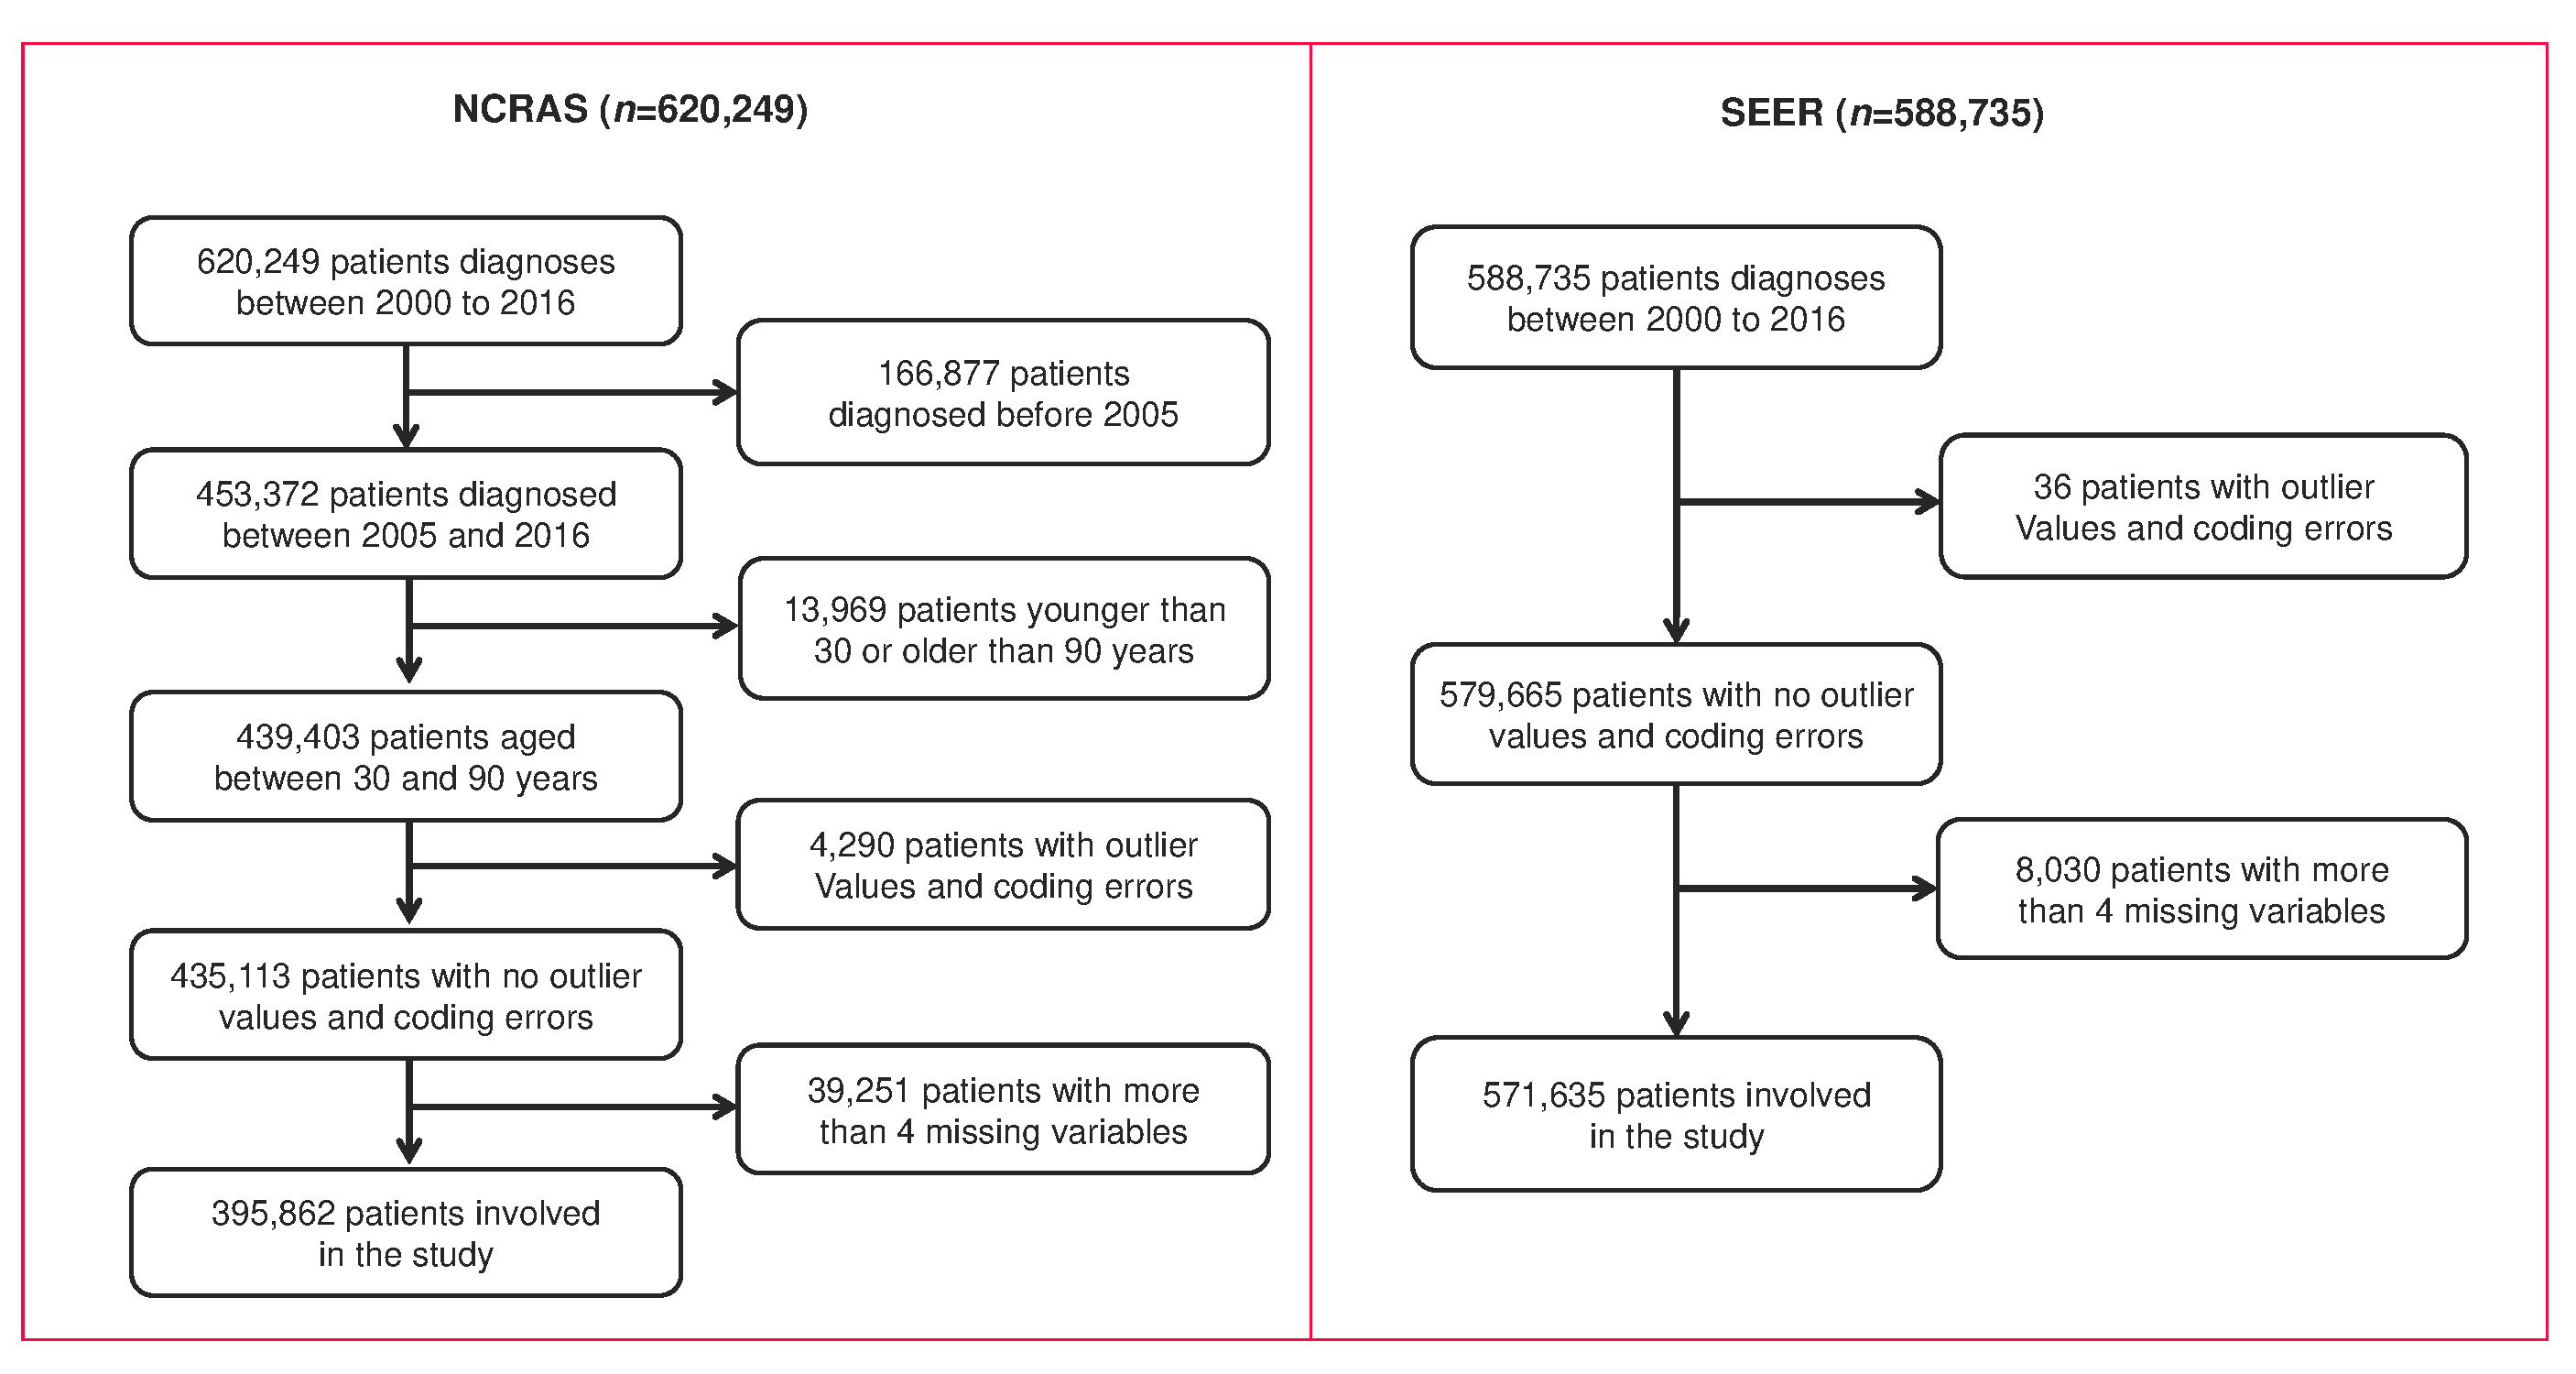
\includegraphics[width=8.75in]{ch8Fig1.pdf}
   \caption{Flow charts for the sample selection and patient inclusion process.}
    \label{ch8fig1}
\end{sidewaysfigure} 

\subsection{Outcomes}
The primary outcome of interest for prognostication was survival from all-cause mortality with and without adjuvant therapies at 3, 5 and 10 years after surgery for breast cancer. All-cause mortality was further subdivided into breast cancer related mortality, which was assessed as a secondary outcome, and mortality due to other causes. Breast cancer related mortality was defined as ICD-10 code C.50 listed on the death certificate as a cause of death, whereas mortality due to other causes was defined as any other ICD-10 code. 

\subsection{Missing Data Imputation}
A limitation of existing models has been their dependence on complete case analysis, and lack of flexibility to incorporate missing variables. Our analysis suggested that missingness was highly informative\cite{ware2012missing}; (log-rank test for difference in 5-year survival between patients with complete data and one or more missing variable, $p < 0.001$). In this context, including only patients with complete data is likely to affect model generalisability. Therefore, in the interest of generalisability, we opted to impute any missing data using data available on other variables. For all study cohorts, we imputed missing data using using the model-based multiple chained equations\cite{zhang2016multiple} (MICE) method. We tested the robustness of the model to missing data in sensitivity analyses, as discussed subsequently. 

\section{Model Development using AutoPrognosis}
\label{ch8sec2}
AutoPrognosis was used to automatically construct an optimized prognostic model fit to the dataset at hand by tuning the parameters of an ensemble of 20 state-of-the-art machine learning models (such as gradient boosting and deep neural networks). The overall Adjutorium model was constructed by fitting 10 binary classification models (optimized via AutoPrognosis) to predict outcomes at 10 distinct knots (time horizons spanning from 1 to 10 years from baseline, with 1-year increments). Survival curves were created by smoothing the predictions at the 10 knots by fitting the discrete predictions to a Weibull survival function. We used the symbolic metamodeling methodolgy presented in Chapter 3 to convert the trained ensemble model into an understandable mathematical equation that links patient variables to predicted outcomes. An illustrative schematic of AutoPrognosis is provided in Figure \ref{ch8fig2}. 

\afterpage{\clearpage}
\begin{sidewaysfigure}[h]
   \centering
   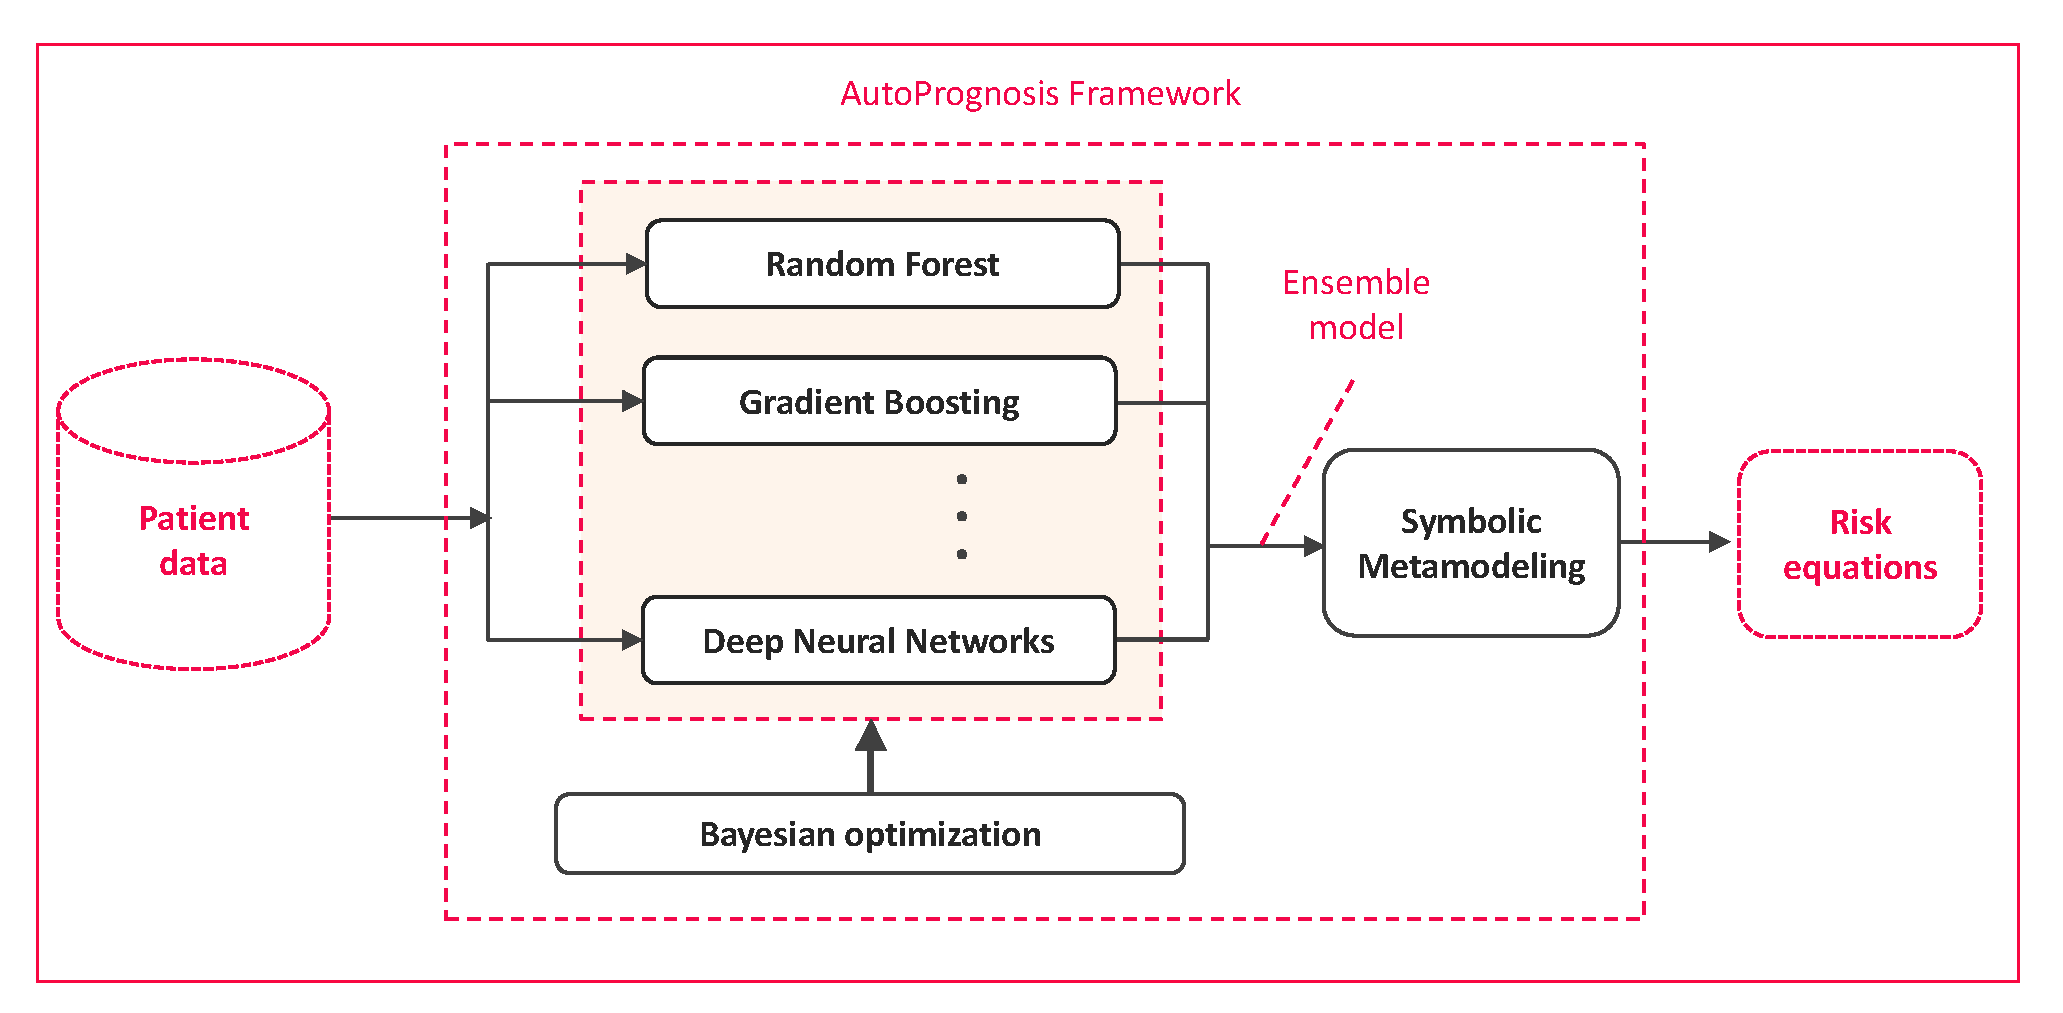
\includegraphics[width=8.75in]{ch8Fig2.pdf}
   \caption{{\bf Schematic depiction for the AutoPrognosis framework.} Given patient data, AutoPrognosis uses a Bayesian optimization algorithm to search for the optimal parameters of a collection of machine learning models and the optimal weight assigned to each model in an ensemble. (Here, we depict random forests, gradient boosting  and neural network models as exemplary elements of the ensemble.)  After fitting the ensemble model, a symbolic regression algorithm is used to convert the fitted model into a mathematical equation that maps patient variables to predicted risk.}
    \label{ch8fig2}
\end{sidewaysfigure}

\section{Statistical Analysis}
\label{ch8sec3}
\subsection*{Comparison with Cox Proportional Hazards Model}
A standard Cox proportional hazards (PH) model fit on the same data as Adjutorium was also assessed for comparison. Consistent with previous methods,\cite{dos2017updated} we applied two separate models, with different baseline hazards for ER positive and ER negative cancer. We included an age squared term to allow for non-linear effects of baseline age at diagnosis on breast cancer mortality.

\subsection*{Model Training, Internal and External Validation}
Patient samples from the NCRAS database were randomly split into two mutually exclusive cohorts: a training cohort of 316,690 patients used for model derivation, and an internal validation cohort of 79,172 patients used to evaluate model accuracy. The entire SEER cohort (571,635 patients) was reserved for external validation. We trained Adjutorium using the NCRAS training data to predict breast cancer and all-cause mortality without adjuvant therapies by adjusting survival times for treatment effects, to create a counterfactual ``untreated'' survival cohort. The estimated survival time in the absence of treatments was calculated as:
\[S^{T=0}_{bc} = S^{T=1}_{bc} \times HR,\]
where $S_{bc}$ represents the uncensored survival time for each individual, $T$ is the indicator for treatment, and $HR$ is the hazard ratio associated with a specific treatment based on the EBCTCG meta-analysis.\cite{early2012comparisons} This is consistent with previous approaches used to create adjusted counterfactual survival times in cross-over trials.\cite{latimer2019two} The same procedure was applied to the Cox PH model.

We conducted internal and external validation of Adjutorium within the NCRAS validation cohort ($n$=79,172) and the SEER cohort ($n$=571,635), respectively. We validated predicted outcomes in the original unadjusted cohort, incorporating treatment effects for patients that had received a given therapy. Using this approach allowed us to evaluate the composite predictive accuracy as well as treatment effects. As breast cancer mortality and mortality from other causes are competing causes, overall survival probability from all causes was calculated as follows:
\[P_{all}(t) = P_{bc}(t) \times P_{nbc}(t).\]
Here, $P_{all}(t)$, $P_{bc}(t)$ and $P_{nbc}(t)$ represent overall survival, survival from breast cancer, and survival from other non-breast cancer related causes at time horizon $t$, respectively. For individuals on adjuvant therapy, $P_{bc}(t)$ was calculated as a function of survival without treatment $P^{T=0}_{bc}(t)$ (as predicted by the trained model), and the effect of treatment, as follows:
\[P^{T=1}_{bc}(t) = \left(P^{T=0}_{bc}(t)\right)^{HR}.\]

\subsection*{Performance Evaluation}

{\it Discriminative Accuracy.} We compared the discriminative accuracy of Adjutorium in predicting all-cause and breast cancer-specific mortality at 3, 5 and 10 years from baseline relative to PREDICT v2.1,\cite{dos2017updated} the Nottingham Prognostic Index (NPI),\cite{fong2015nottingham} and the in-house Cox PH model fitted to the NCRAS training cohort. We assessed the discriminative accuracy of Adjutorium using the time-dependent area under receiver operating characteristic curve\cite{lambert2016summary} (AUC-ROC), Harrell’s concordance index\cite{harrell1996multivariable} (C-index), and Uno’s C-index.\cite{uno2011c} For all evaluations, 95$\%$ confidence intervals were obtained using bootstrapped re-sampling.\\ 
\\
{\it Calibration.} We evaluated the calibration curves of Adjutorium by comparing predicted risk of mortality with observed risk in the cohort at the time horizons of interest. For each time horizon, we divided the risk ranges predicted by Adjutorium into 10 quantiles, and within each quantile, we estimated the observed risk in the corresponding patient samples using a Kaplan-Meier estimator.\cite{d2003evaluation} Calibration curves were evaluated by plotting the predicted risks by Adjutorium on the $x$-axis, and plotting the corresponding observed risk on the $y$-axis.\\
\\
{\it Sensitivity analyses.} In order to examine the robustness of Adjutorium to missingness, we validated its performance separately on individuals with complete data and those with at least one missing variable. Moreover, in order to assess the robustness of Adjutorium to time-cohort effects, due to changes in patient management and survival over time, we also compared the discriminative accuracy of our model with that of PREDICT v2.1 in subsets of patients diagnosed within 1-year windows spanning from 2005 to 2016.\\ 
\\
{\it Subgroup analyses.} We validated Adjutorium within specific patient subgroups stratified by age, ER status, HER2 status, tumour size and tumour grade. We specifically assessed the performance of Adjutorium relative to PREDICTv2.1 in patients aged more than 65 years, patients with larger tumours, and patients with negative ER status. Error counts in each subgroup were obtained through decision thresholds that maximize the Youden J-statistic for each model. To assess the prognostic value of each variable, we also evaluated the predictive ability of each individual variable within each subgroup by re-fitting the machine learning model with one variable at a time.

\section{Results}
\label{ch8sec4}

\textit{Adjutorium Model Development.} A high-level illustration for the machine learning model generated by AutoPrognosis when fitted to the development cohort ($n$=316,690) is provided in Figure \ref{ch8fig3}. The overall model comprised an ensemble of four binary classification models\cite{kotsiantis2007supervised}: random forest, neural network, gradient boosting, and AdaBoost. The prediction issued by Adjutorium is a weighted combination of the predictions of the four members of the ensemble in Figure \ref{ch8fig3}.

The risk equation that maps patient variables to breast-cancer-related and non-breast-cancer-related survival curves (i.e., $P_{bc}(t)$ and $P_{nbc}(t)$) are visualized in Figure \ref{ch8fig4}. For a given patient, the breast-cancer-related survival probability is given by $P_{bc}(t) = 1/(1 + \exp(-\lambda_{bc}(t)))$, where $t$ is the time horizon at which the survival probability is evaluated. The term $\lambda_{bc}(t)$ can be interpreted as the {\it odds ratio} for survival at time $t$, and is decomposed as follows:
\[\lambda_{bc}(t) = \underbrace{\bar{\lambda}_{bc}(t)}_{\mbox{\footnotesize Population-level}} + \underbrace{\bar{\lambda}^{G, ER}_{bc}(t)}_{\mbox{\footnotesize Grade-ER-specific}},\]
where the first term $\bar{\lambda}_{bc}(t)$ is shared among all patients in the population, and includes the non-linear effects of the age and number of lymph nodes variables, in addition to interaction terms between age, mode of detection, tumour size and number of lymph nodes (Figure \ref{ch8fig4}). The second term $\bar{\lambda}^{G, ER}_{bc}(t)$ includes linear contributions of all prognostic variables, with coefficients that are specific to every possible combination of tumour grade and ER status. The risk equations in Figure \ref{ch8fig4} demonstrate that our machine learning approach identified new interactions that were not incorporated in previous models\cite{dos2017updated}, namely the interactions between tumour grade and all other prognostic factors. The risk equation for $P_{nbc}(t)$ is similar to that of $P_{bc}(t)$.

\afterpage{\clearpage}
\begin{sidewaysfigure}[h]
\centering
   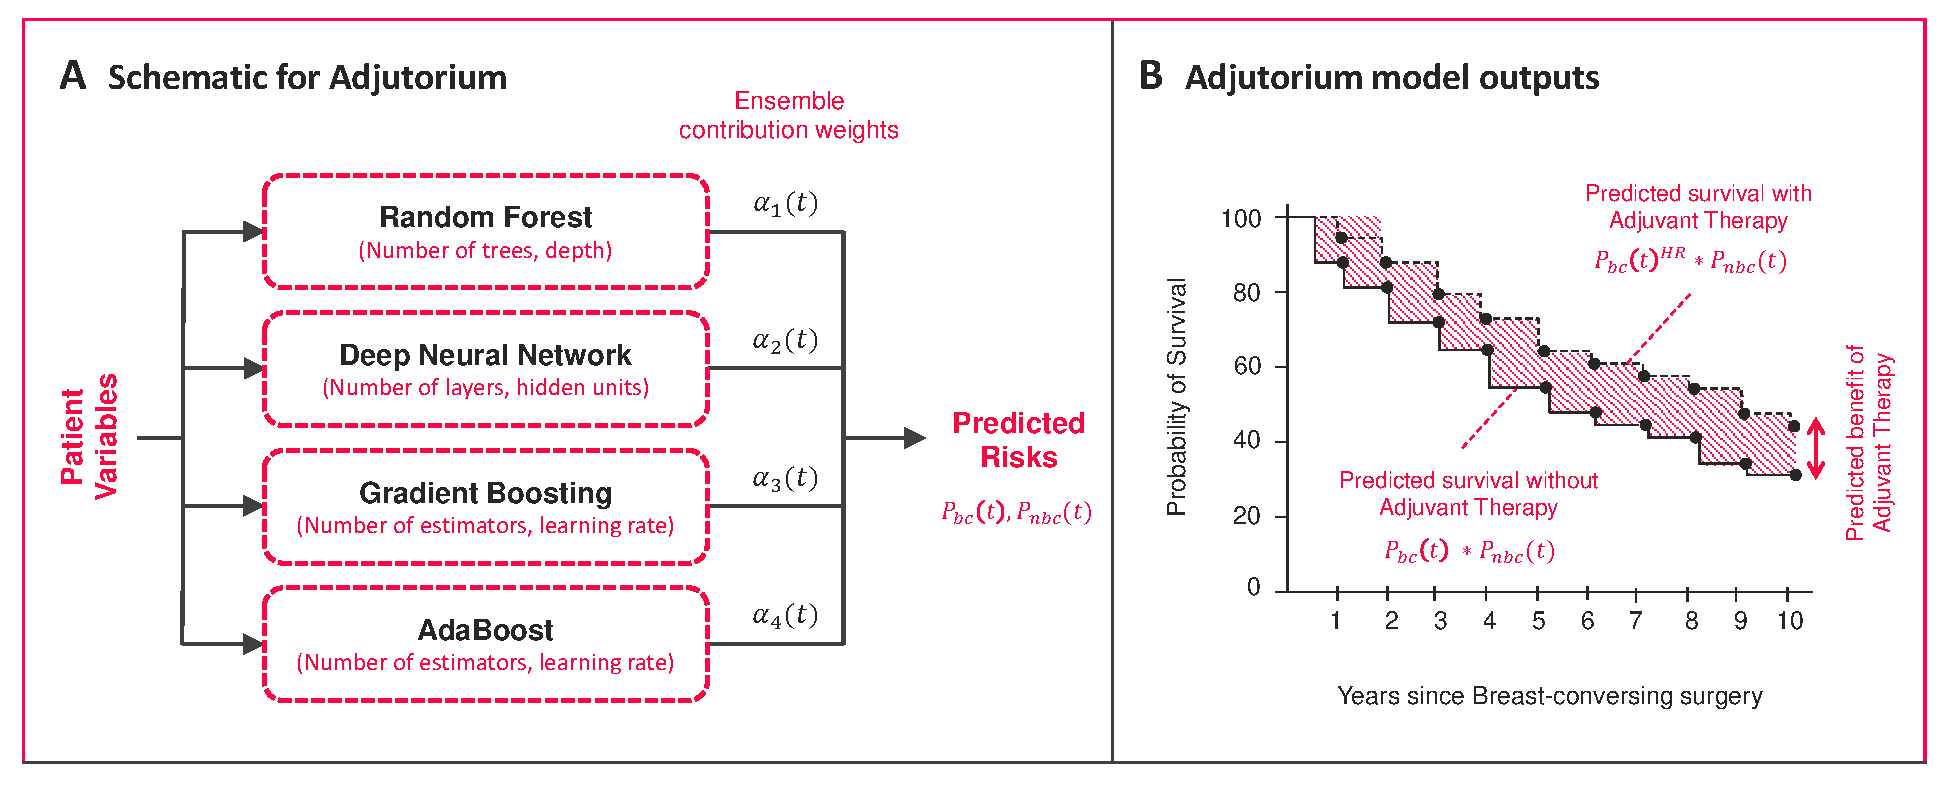
\includegraphics[width=9in]{ch8Fig3.pdf}
    \caption{{\bf Illustration for the machine learning model underlying Adjutorium.} Panel A displays the model learned by the AutoPrognosis framework. The overall model comprises an ensemble of four basic machine learning models: random forest, neural network, gradient boosting, and AdaBoost. The prediction issued by Adjutorium is a weighted combination of the predictions issued by each of the four members of the ensemble. Each model in the ensemble has a set of parameters (listed between brackets in Panel A), and an assigned weight $\alpha(t)$ determining its contribution in the final risk prediction. Both the model parameters and its weight change depending on the prediction horizon $t$. The predicted survival curve for an exemplary patient (with and without adjuvant therapy) is shown in Panel B. Here, each prediction horizon (1 to 10 years since diagnosis, with 1-year steps) corresponds to a knot in the survival curve, and each knot is associated with a distinct set of model parameters and contribution weights in the ensemble in Panel A.}
    \label{ch8fig3}
\end{sidewaysfigure} 

\afterpage{\clearpage}
\begin{sidewaysfigure}[h]
\centering
   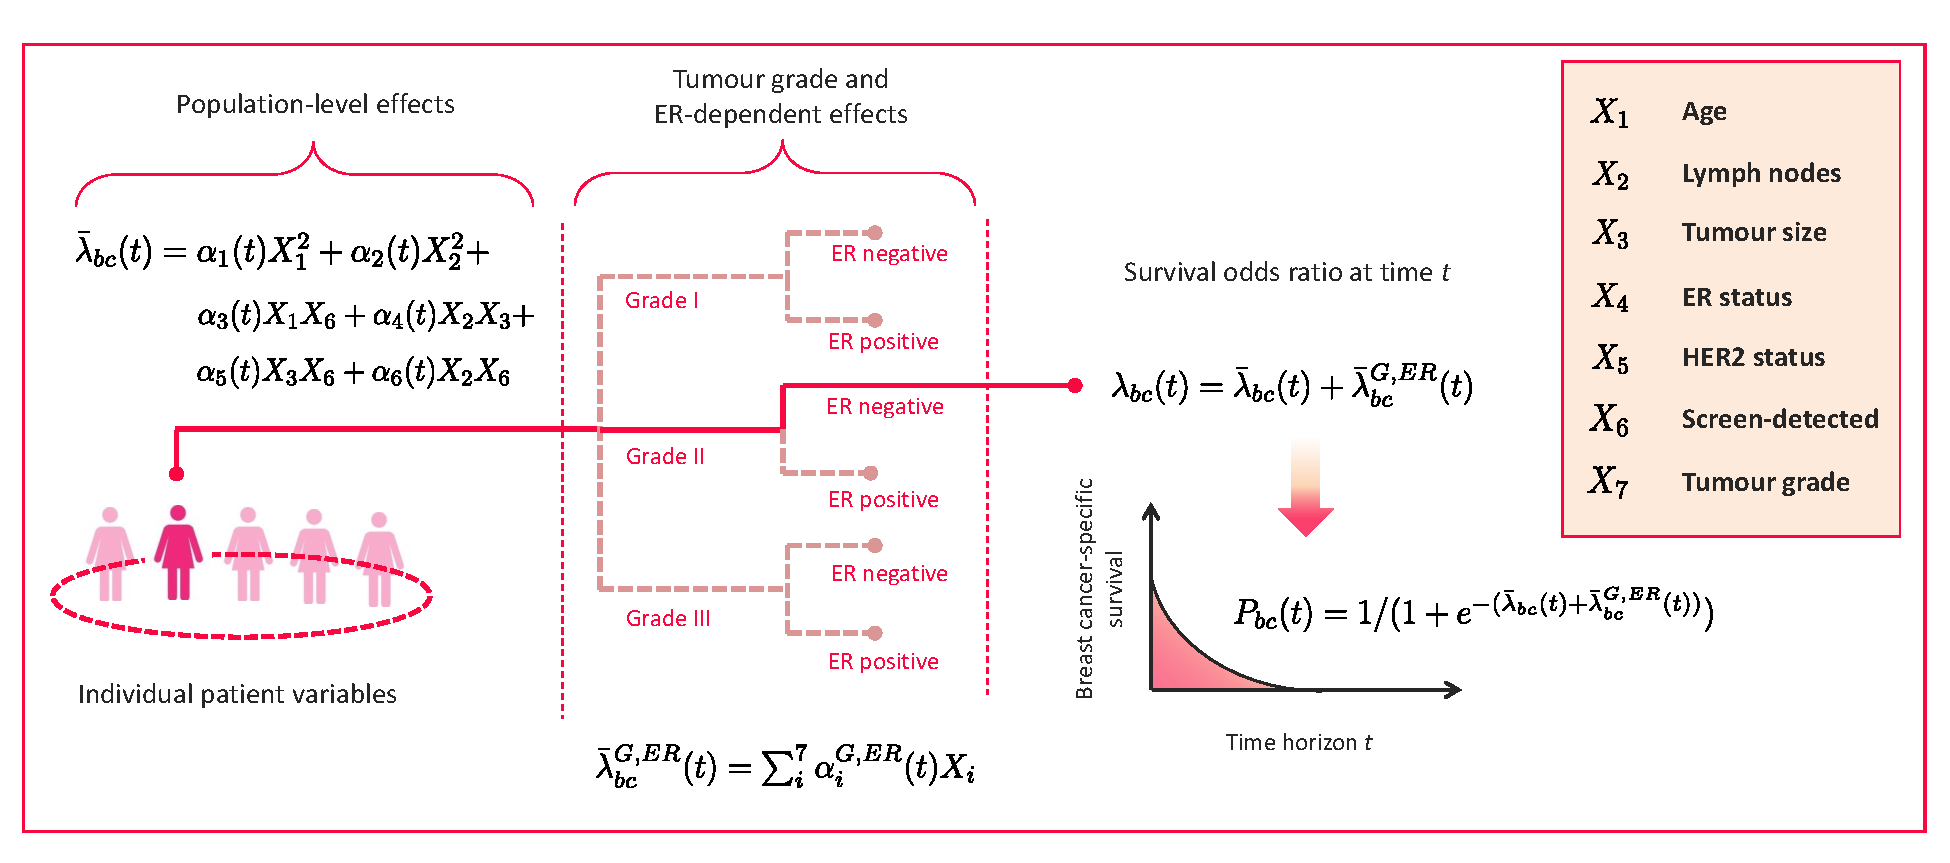
\includegraphics[width=9in]{ch8Fig4.pdf}
    \caption{{\bf Risk equations underlying Adjutorium.} Given the individual-level variables of a patient, the risk equation evaluates a survival curve corresponding to the probability of survival at future time horizons. The odds ratio for survival at time $t$ is decomposed into two components: (1) a population-level term that models non-linear effects of age and number of lymph nodes, in addition to interactions between different variables using six coefficients that are fixed for all patients, and (2) a tumour grade and ER-specific term that evaluates the linear effects of all prognostic factors with coefficients that are specific to every group of patients with the same grade and ER status. Here we show an exemplary patient with ER negative cancer and tumour grade 2 and. The risk equation above is an abstraction for the predictions issued by the machine learning model in Figure \ref{ch8fig3} that ensure the model's interpretability and transparency.}
    \label{ch8fig4}
\end{sidewaysfigure} 

{\it Discriminative Accuracy.} Adjutorium uniformly outperformed PREDICT v2.1, NPI, and the conventional Cox PH model in predicting all-cause and breast cancer-specific mortality, both when validated internally within NCRAS (Table \ref{ch8Table1}), and externally within the SEER cohort (Table \ref{ch8Table2}). The improvements were achieved with respect to all discriminative accuracy metrics and all time horizons under study. 

\afterpage{\clearpage}
\begin{sidewaysfigure}[h]
\centering
   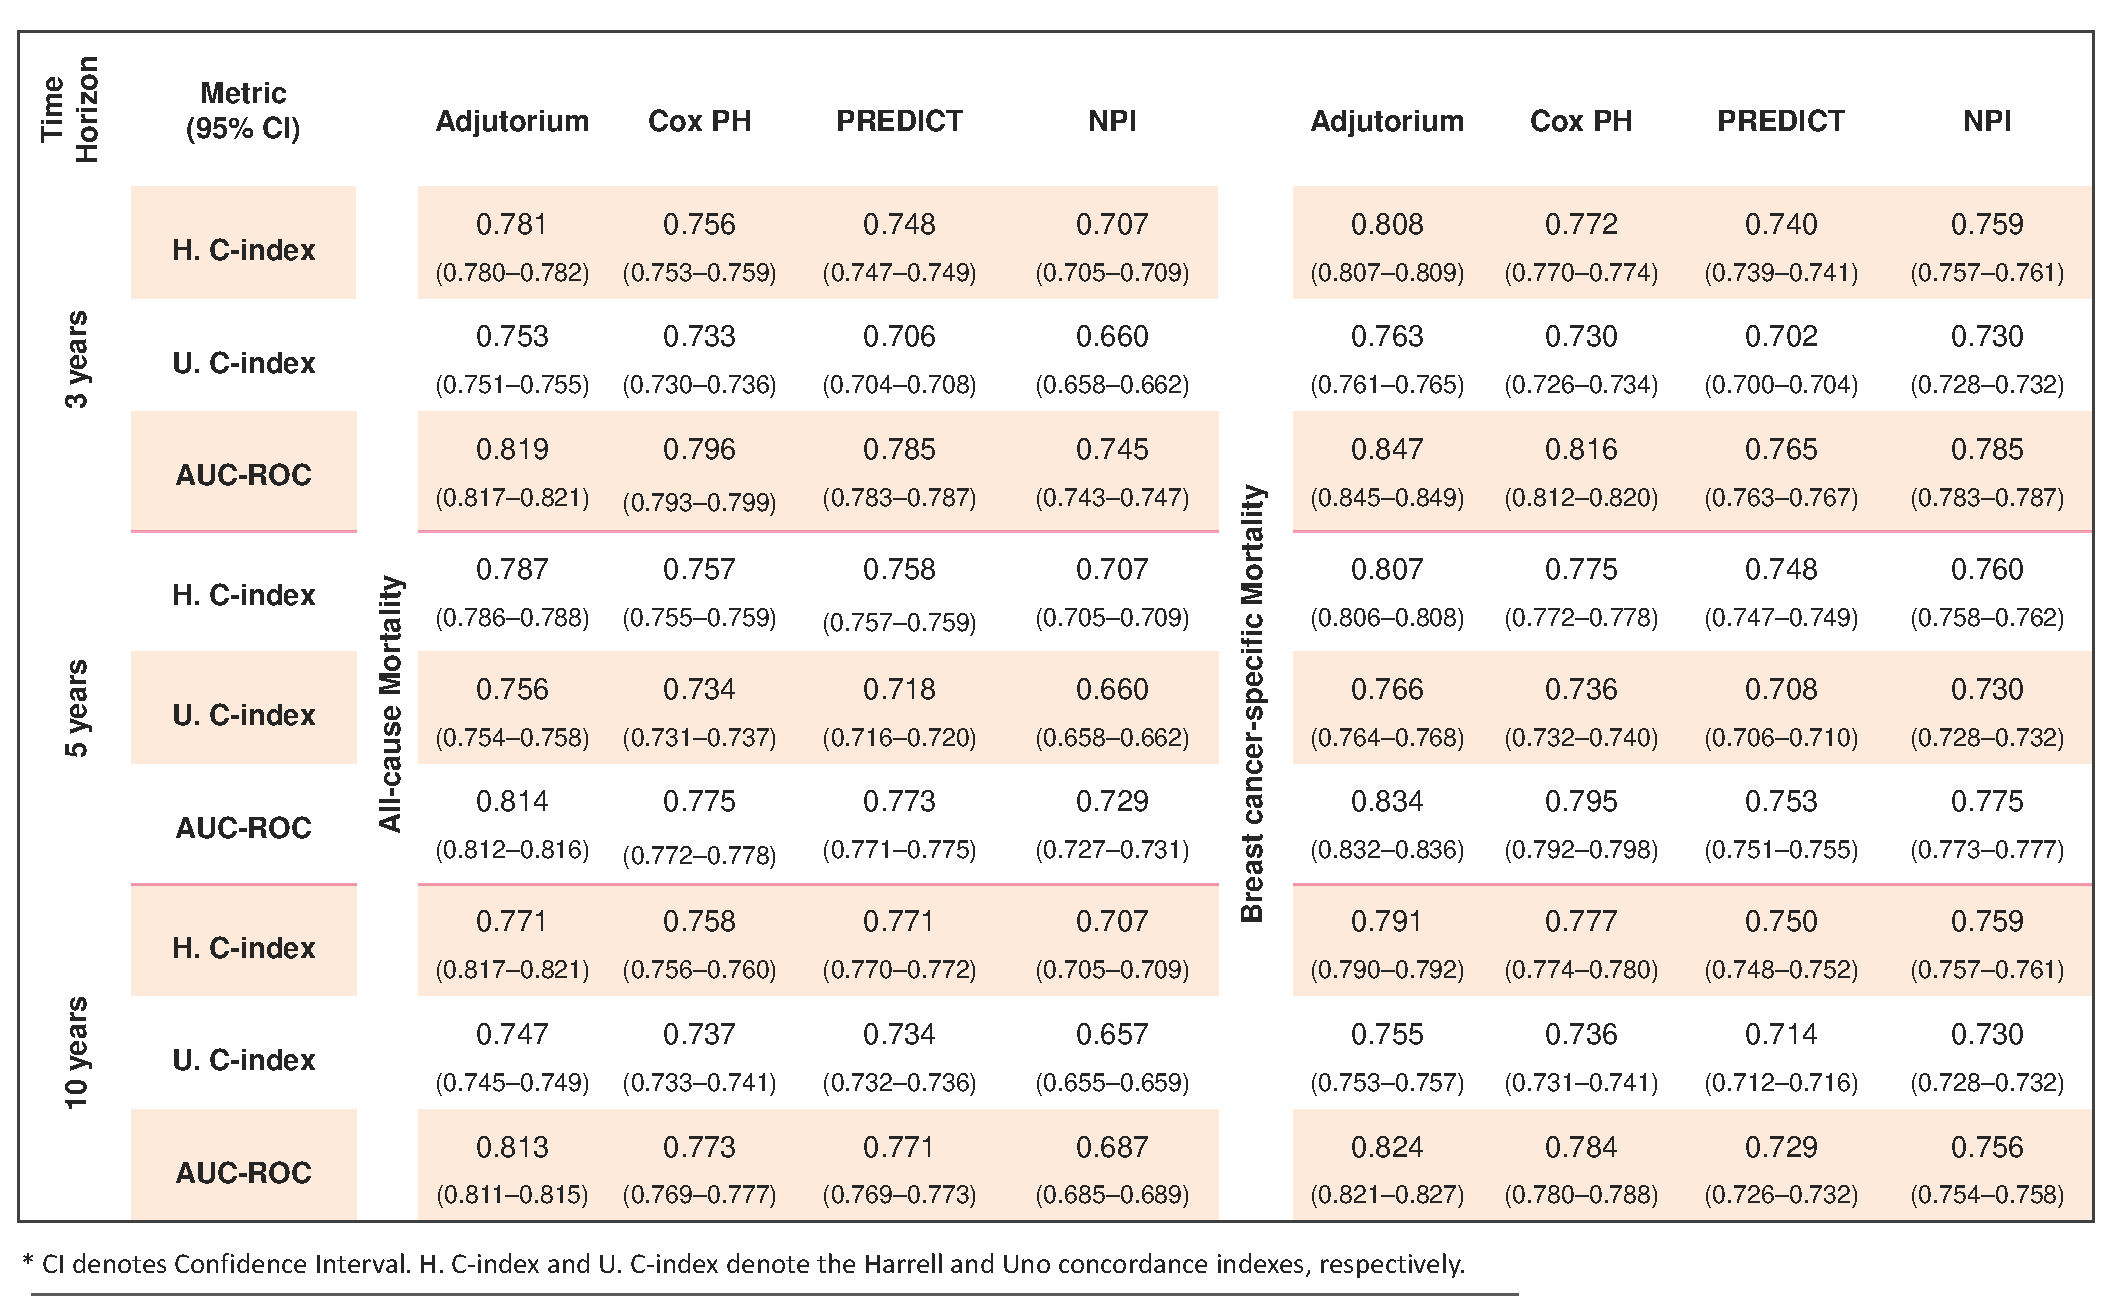
\includegraphics[width=9in]{ch8Table1.pdf}
    \caption{Discriminative Accuracy with Respect to the Primary and Secondary Outcomes in the Internal Validation Cohort (NCRAS, $n$=79,172).*}
    \label{ch8Table1}
\end{sidewaysfigure}

\afterpage{\clearpage}
\begin{sidewaysfigure}[h]
\centering
   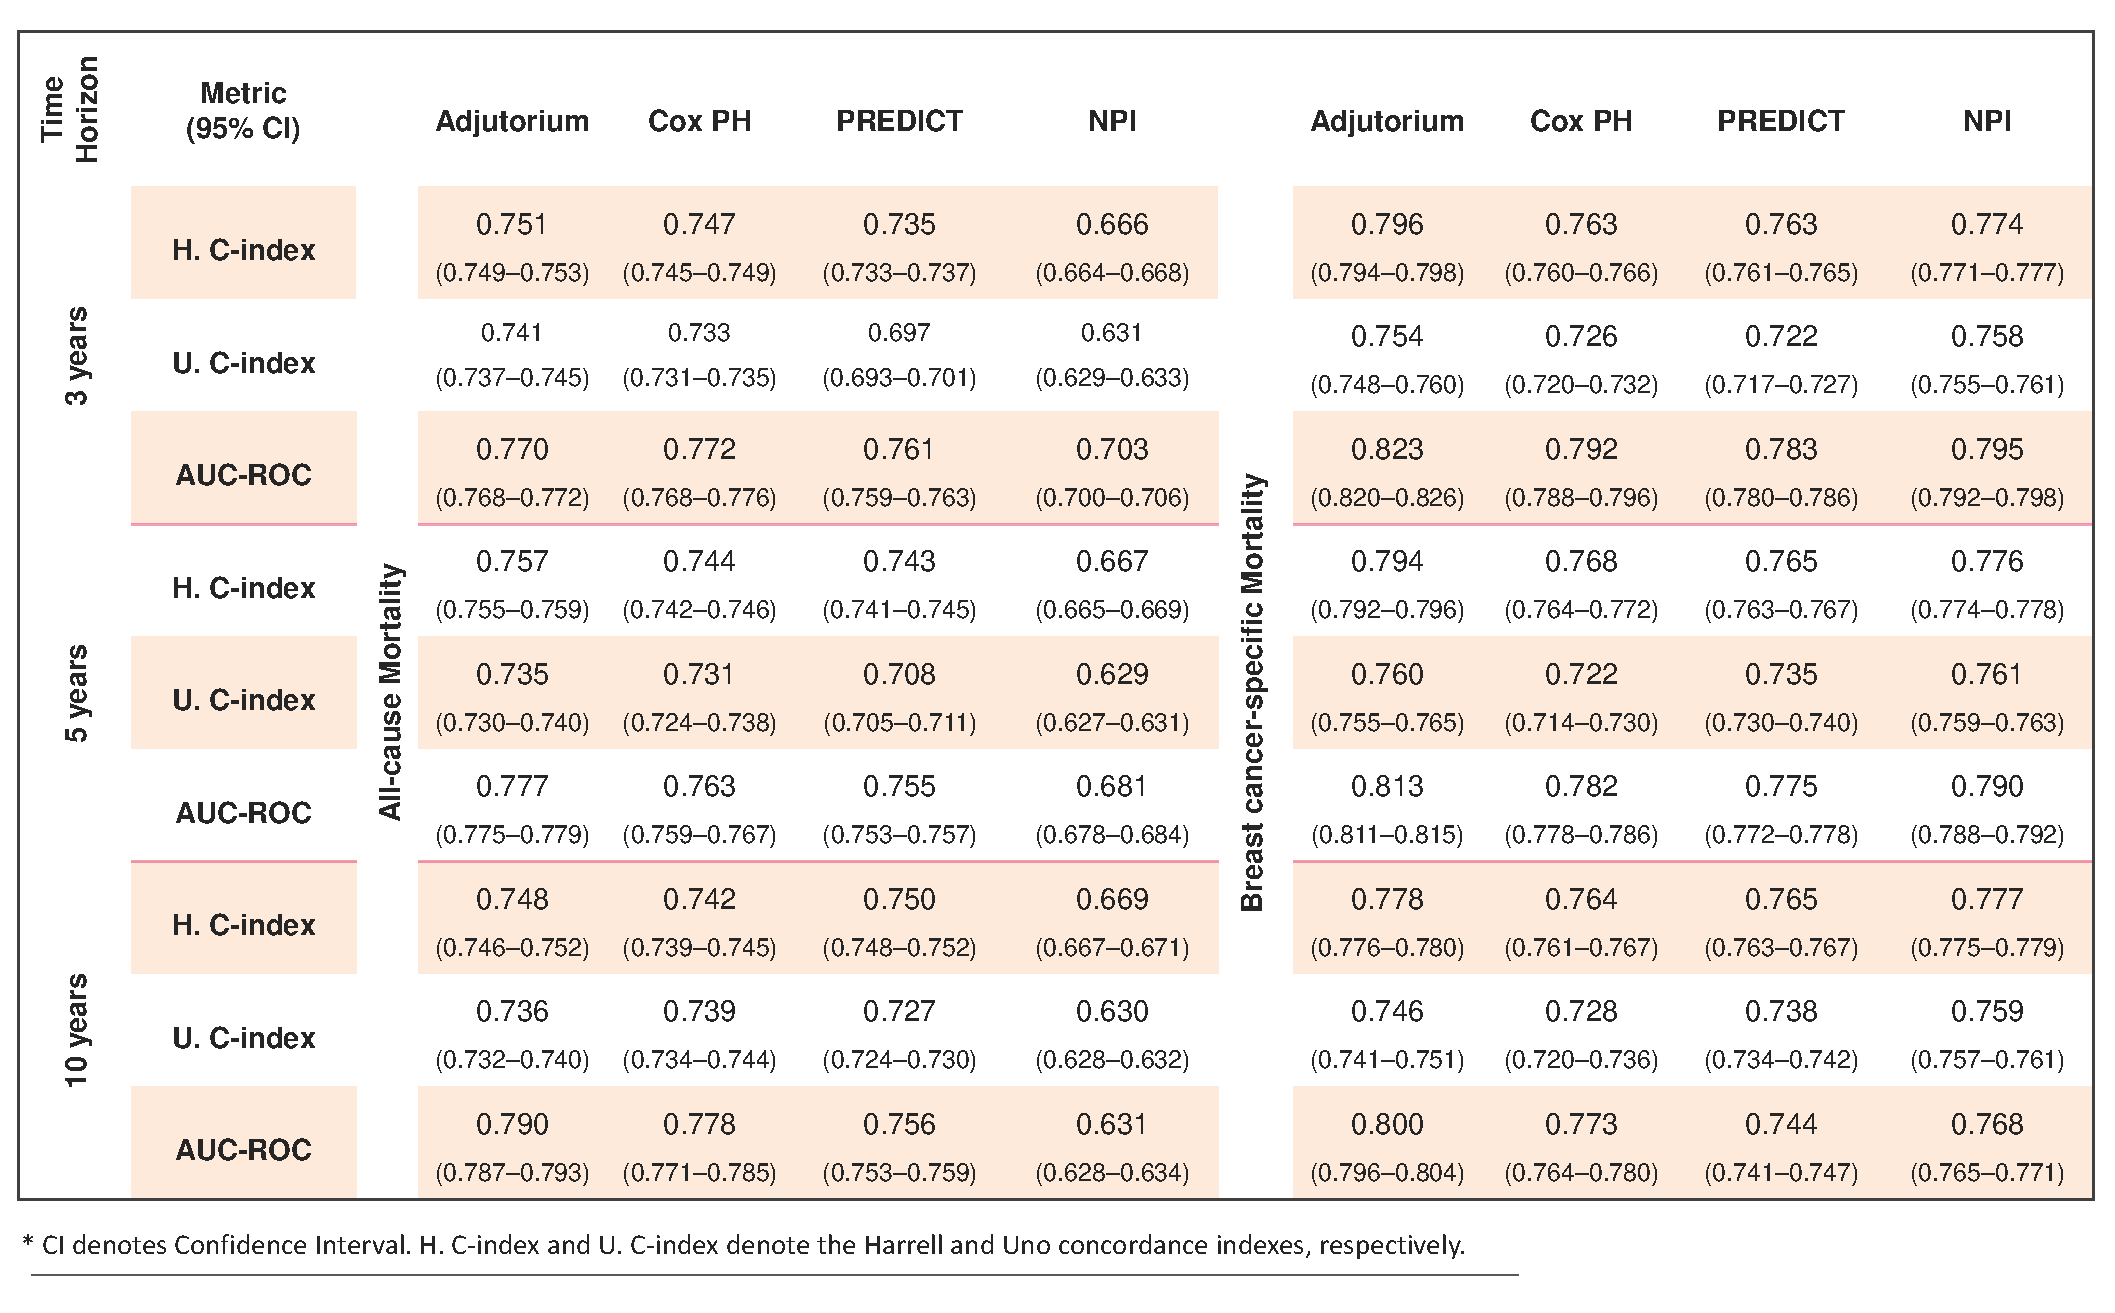
\includegraphics[width=9in]{ch8Table2.pdf}
    \caption{Discriminative Accuracy with Respect to the Primary and Secondary Outcomes in the External Validation Cohort (SEER, $n$=571,635).*}
    \label{ch8Table2}
\end{sidewaysfigure}

\afterpage{\clearpage}
\begin{sidewaysfigure}[h]
\centering
   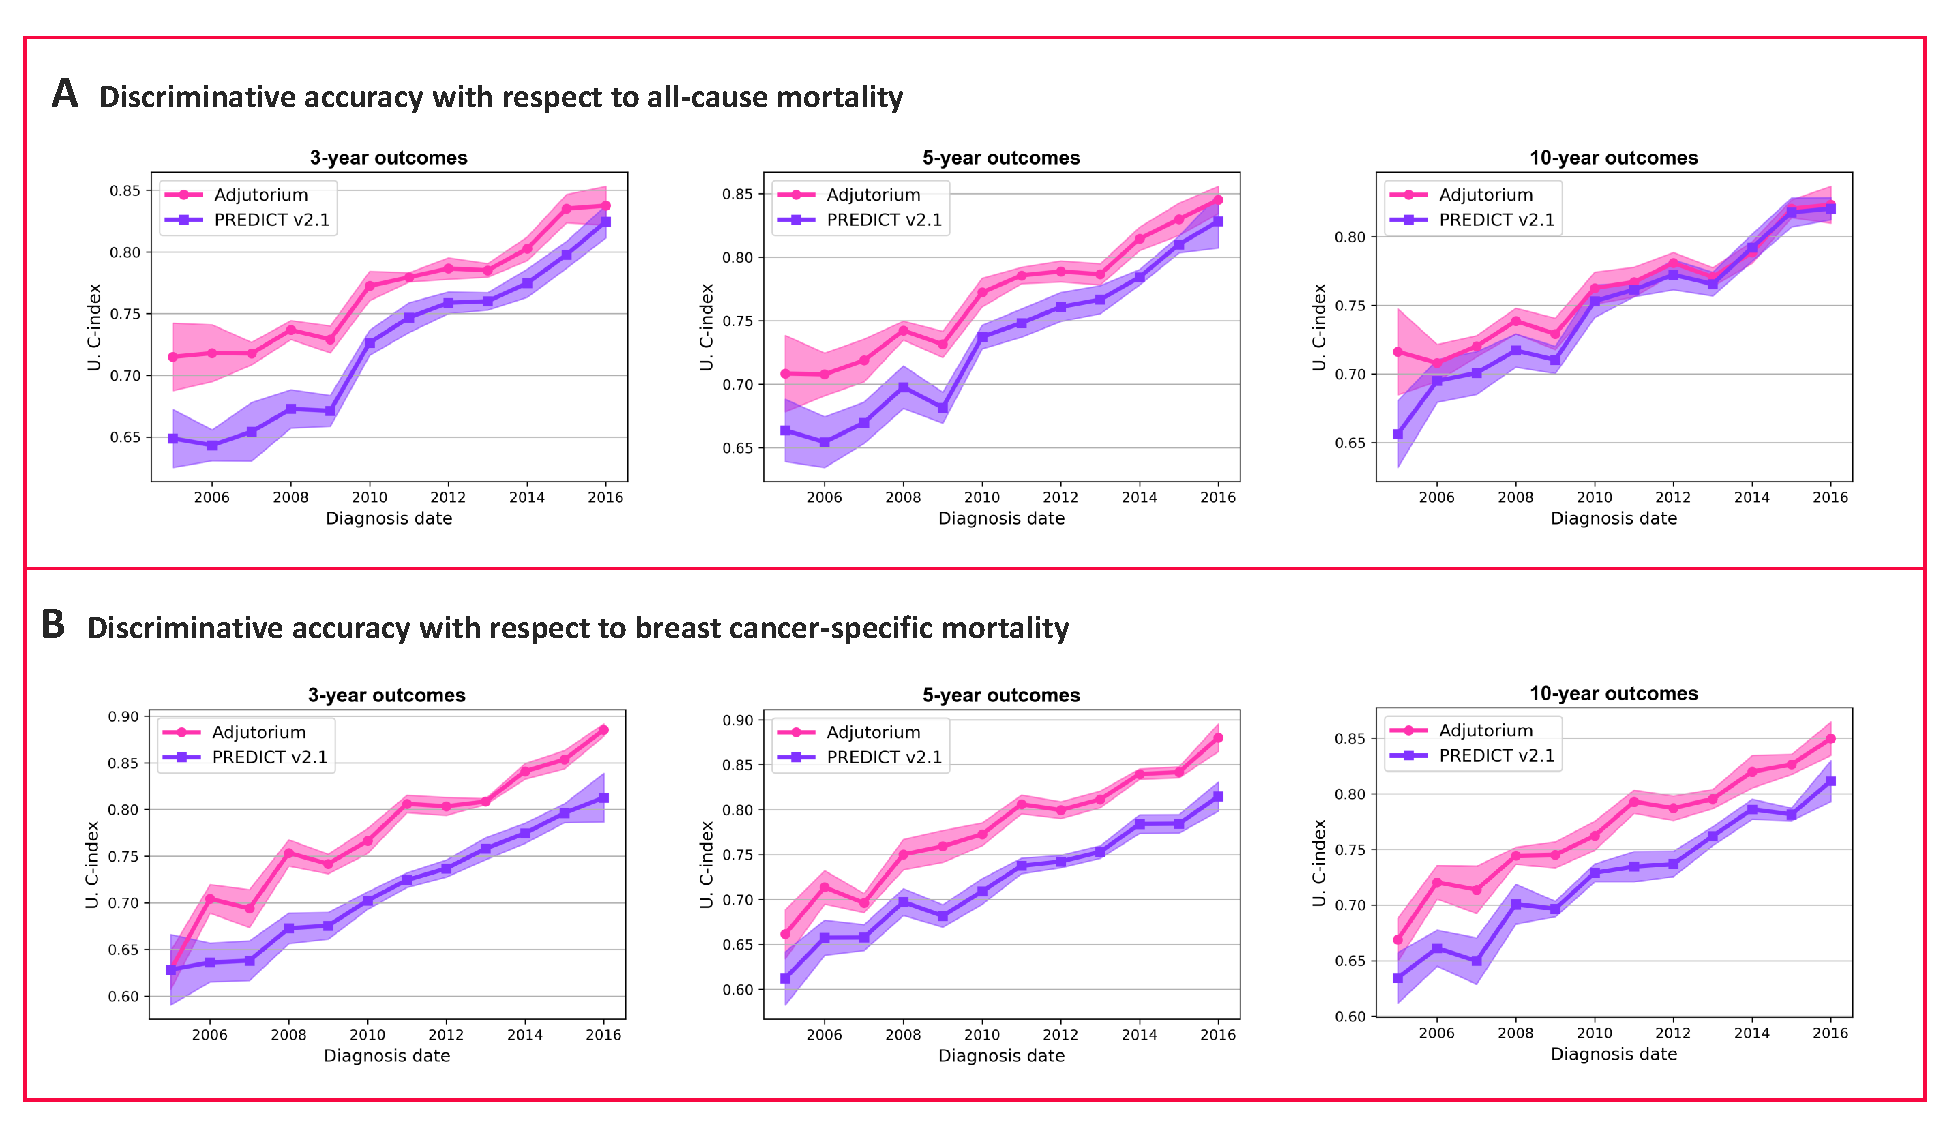
\includegraphics[width=9in]{ch8Fig5.pdf}
    \caption{Discriminative accuracy evaluated in sub-cohorts of patients stratified by diagnosis date.}
    \label{ch8fig5}
\end{sidewaysfigure}

In internal validation, Adjutorium predicted 10-year all-cause mortality with an AUC-ROC accuracy of 0.813 (95$\%$ CI: 0.811-0.815), compared with 0.771 (95$\%$ CI: 0.769-0.773) by PREDICT v2.1, 0.687 (95$\%$ CI: 0.685-0.689) by NPI, and 0.773 (95$\%$ CI: 0.769-0.777) by the Cox PH model. Similar performance gains were achieved over the other time horizons, and with respect to the C-index statistic (Table \ref{ch8Table1}). The improvements in accuracy achieved by Adjutorium were even more significant in predicting breast cancer-specific mortality, with an AUC-ROC of 0.824 (95$\%$ CI: 0.821-0.827) for 10-year outcomes, compared with 0.729 (95$\%$ CI: 0.726-0.732) by PREDICT v2.1, 0.756 (95$\%$ CI: 0.754-0.758) by NPI, and 0.784 (95$\%$ CI: 0.780-0.788) by the Cox PH model. The fact that the accuracy improvements were more significant in the secondary outcome is not surprising since all of the variables included in the model were breast cancer-related.

Adjutorium generalized well to the external validation cohort, with similar accuracy improvements for both the primary and secondary outcomes (Table \ref{ch8Table2}). With respect to 10-year all-cause mortality, Adjutorium achieved an AUC-ROC of 0.790 (95$\%$ CI: 0.787-0.793), compared to 0.756 (95$\%$ CI: 0.753-0.759) by PREDICT, 0.631 (95$\%$ CI: 0.628-0.634) by NPI, and 0.778 (95$\%$ CI: 0.771-0.785) by the Cox PH model. Similar gains were achieved over the other time horizons (Table \ref{ch8Table2}). For prediction of 10-year breast cancer-specific mortality, Adjutorium achieved an AUC-ROC of 0.800 (95$\%$ CI: 0.796-0.804), compared to 0.744 (95$\%$ CI: 0.741-0.747) by PREDICT, 0.768 (95$\%$ CI: 0.765-0.771) by NPI, and 0.773 (95$\%$ CI: 0.764-0.780) by  Cox PH model.  

Importantly, Adjutorium outperformed the Cox PH model fitted to the same development cohort, reflecting the {\it gain from modeling}, i.e., the gain achieved by using flexible machine learning models instead of standard regression. On the other hand, the gain achieved by the Cox PH model compared to PREDICT v2.1 in external validation reflects the {\it gain from information}, i.e., the gain achieved by using large-scale, representative data that enhance the accuracy and generalizability of the fitted models to other cohorts that might entail different demographic structure and outcomes. \\
\\
\textit{Sensitivity Analysis}. Internal and external validation on patient sample with complete and missing data demonstrated the robustness of Adjutorium to data missingness; the model performed well in cases with complete and missing data, outperforming other models by similar margins in both analyses. When validated on 21,164 patients (in the internal validation cohort) with complete data on all variables, the AUC-ROC accuracy of Adjutorium with respect to 10-year breast cancer-specific mortality was 0.811 (95$\%$ CI: 0.0.808-0.814), and 0.783 (95$\%$ CI: 0.780-0.786) for PREDICT v2.1. When validated on 57,996 patients with missing data on one or more variables, the AUC-ROC accuracy of Adjutorium was 0.829 (95$\%$ CI: 0.0.827-0.831), and 0.728 (95$\%$ CI: 0.725-0.731) for PREDICT v2.1. Adjutorium also displayed robustness to time-cohort effects; internal validation on sub-cohorts stratified by diagnosis dates from 2005 to 2016 showed that the accuracy gains by Adjutorium are achieved for all diagnosis years Figure \ref{ch8fig5}.\\
\\
\textit{Subgroup Analysis}. The accuracy improvements achieved by Adjutorium were consistent across all subgroups of patients stratified by age, HER2 status, ER status and tumour grade (Table \ref{ch8Table3}). Improvements were greater in subgroups that are poorly served by current prognostic tools; the accuracy gains achieved by Adjutorium relative to PREDICT v2.1 were higher in elderly patients (age $>$ 65 yrs at diagnosis), patients with ER negative and HER2 negative breast cancer (Table \ref{ch8Table3}), and patients with large tumours. This is likely due to the fact that data-driven machine learning captured nuanced interactions and non-linear patterns that were not incorporated in existing prognostic tools. 

\afterpage{\clearpage}
\begin{sidewaysfigure}[h]
\centering
   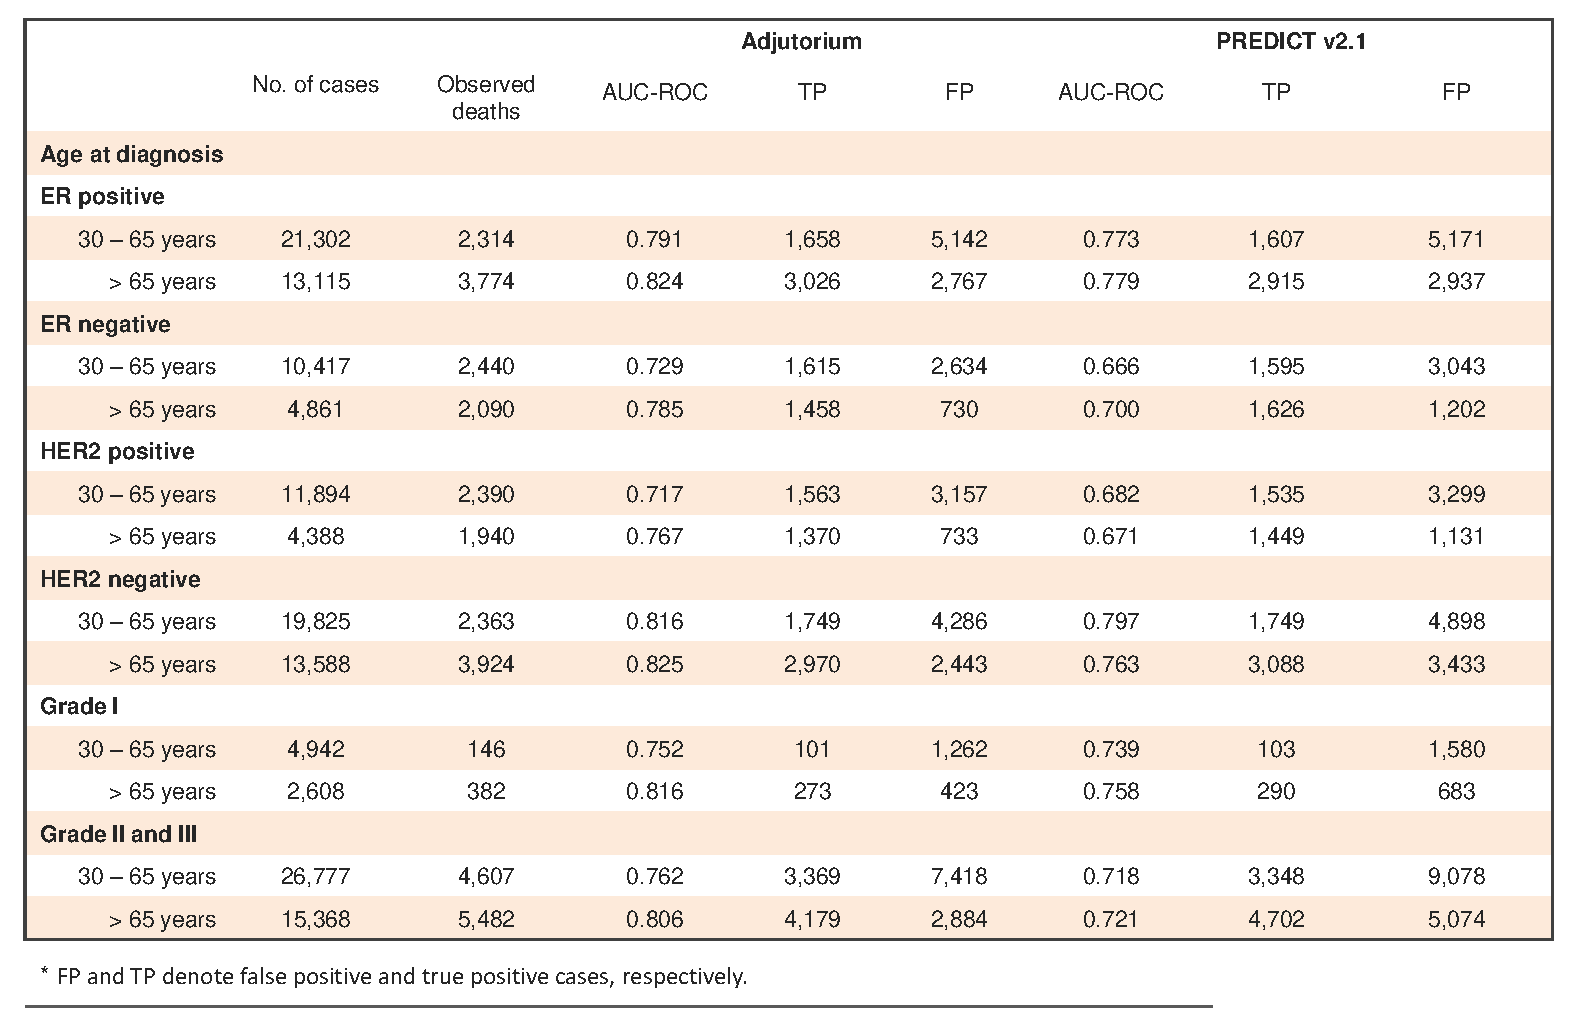
\includegraphics[width=9in]{ch8Table3.pdf}
    \caption{Subgroup-level Discrimination with Respect to Breast cancer-specific 10-year Outcomes in Internal Validation*.}
    \label{ch8Table3}
\end{sidewaysfigure}

\section{Discussion and Conclusions}
In this Chapter, we developed and validated Adjutorium --- a machine learning-based tool for predicting the individualized benefit of adjuvant therapies in breast cancer based on the AutoPrognosis framework presented in Chapter 4. Involving data from nearly 1 million individuals with breast cancer from the UK and US, this is one of the largest studies of its kind. We found that Adjutorium substantially outperforms one of the most widely used standards for clinical decision making, and critically is generalisable to distinct clinical settings. To our knowledge this is the first application of a machine learning model for prognostication in breast cancer, that has been shown to be generalisable across multiple nationally representative cohorts. 


While several prognostication methods are available for supporting clinical decisions regarding adjuvant therapies in breast cancer, they have well recognized limitations particularly in terms of their accuracy in certain subgroups and their generalisability to other populations. We find that Adjutorium outperforms existing clinical decision support tools in terms of accuracy, and calibration to observed outcomes, across all patient groups. Additionally, it shows substantially improved performance in subgroups where existing clinical decision support tools are known perform poorly (e.g., older women with early cancer, HER negative and ER negative breast cancer) suggesting that using Adjutorium to support clinical decisions may lead to better treatment decisions, and potentially better outcomes in these subgroups. By contrast with other existing tools, Adjutorium is robust to missing data, and is able to make accurate predictions even when information on some of the prognostic factors is not available. This is an important advance, making our model more generalisable to settings where data on patients may be incomplete. 

We find that Adjutorium not only outperforms PREDICT v2.1, but also a Cox proportional hazards model fit on the same training cohort. This suggests that gains in performance are achieved not only due to a larger representative set for training the models, but also due to the flexible nature of the machine learning algorithms applied. Our fitted model does not make any assumptions about the linearity of the patient risks as function of prognostic factors, or the proportionality of hazards over time. Additionally it is able to infer interactions, and non-linear associations in a data-driven fashion, as evident through the interpretable risk equations describing the machine learning model. 

We acknowledge limitations of our model, which include the retrospective nature of our study which makes it difficult to assess changes in patient outcomes when using Adjutorium relative to existing tools. Another limitation is that our model does not predict outcomes such as recurrence, and currently does not incorporate gene expression based predictive information. However, these can be easily incorporated into our model. Also, Adjutorium does not explicitly derive treatment effects in a data-driven fashion, rather using estimates from meta-analyses on clinical trials. 


%\chapter{Conclusions}

{
%\openup 0.5em
\bibliographystyle {uclathes} %{unsrt} %
\bibliography {thesisrefs}}    % bibliography references

\end {document}

